\input cinput.tex    \documentclass[12pt,a4paper]{book}
% �N���`�s���W�[�� A.B.C.D
\setcounter{secnumdepth}{4}
% �N subsubsection �[��ؿ�
\setcounter{tocdepth}{3}

%\setcounter{tocdepth}{3}
% �ƪ� index
\usepackage{makeidx}
\makeindex
\usepackage{url}
\usepackage[dvips]{color}
\usepackage{listings}
\usepackage{fancyhdr}
\usepackage{fancyvrb}
\usepackage[dvips]{hyperref}
\usepackage{booktabs}
\usepackage{graphicx}
\usepackage{lastpage}
%\usepackage{verbatim}

%�w�q�ۤv�� page style
\pagestyle{fancy}
\fancyhead[LE]{\leftmark}
\fancyhead[RE]{}
\fancyhead[RO]{\rightmark}
\fancyhead[LO]{}
\fancyhead[CO,CE]{}
\fancyfoot[CO,CE]{}
%\fancyfoot[LE,RO]{\thepage \ of \pageref{LastPage}}
\fancyfoot[LE,RO]{\thepage}
\renewcommand{\footrulewidth}{0pt}

% �w�q \fancypagestyle �`�N % �Ÿ��n�[
\fancypagestyle{plain}{%
\fancyhf{}
\renewcommand{\headrulewidth}{0pt}
\fancyfoot[LE,RO]{\thepage}}
%\renewcommand{\headrulewidth}{0pt}

\headsep=1.5cm
%\includeonly{small_autotools}
\begin{document}
\begin{titlepage}
\begin{figure}
\begin{center}
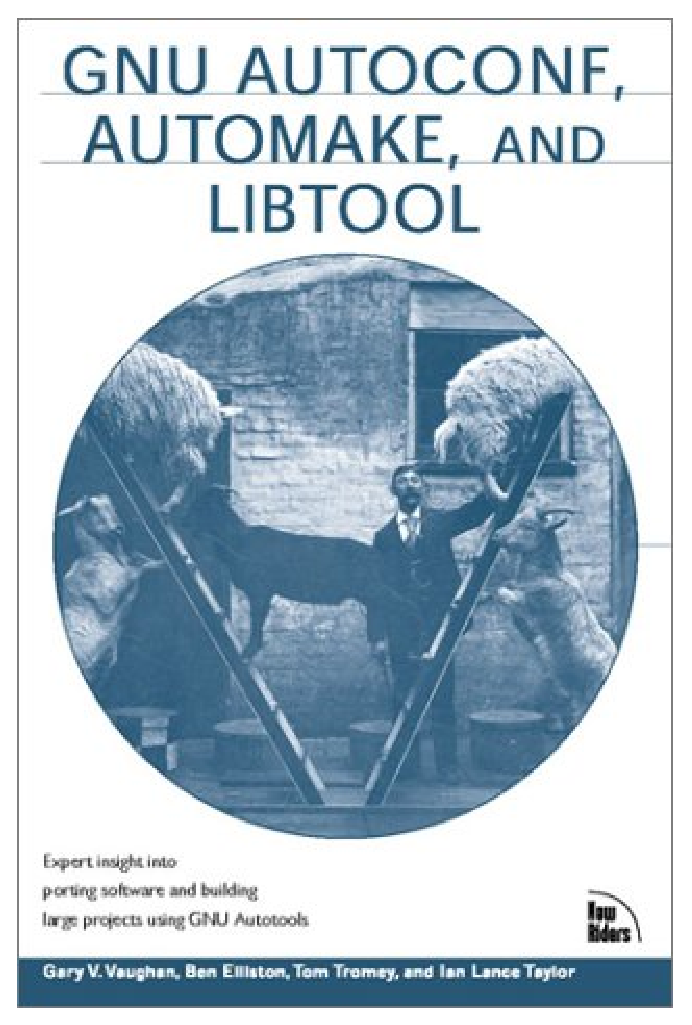
\includegraphics{cover.eps}
\end{center}
\end{figure}
\end{titlepage}


\tableofcontents
\listoftables
\listoffigures
\frontmatter
\thispagestyle{empty}
\chapter{Magic Happens Here}


Do you remember the 1980s? Veteran users of free software on Unix could testify that though there were a lot of programs distributed as source code back then (over USENET), there was not a lot of consistency in how to compile and install it. The more complicated a package was, the more likely it was to have its own unique build procedure that had to be learned first. And there were no widely used approaches to portability problems. Each software author handled them in a different way, if they did at all. 


Fast forward to the present. A de facto standard is in widespread use for solving those problems, and it's not just free software packages that are using it; some proprietary programs from the largest computer companies are built using this software. It even does Windows. 


As it evolved in the 1990s it demonstrated the power of some good ideas: sharing expertise, automating repetitive work, and having consistency where it is helpful without sacrificing flexibility where it is helpful. 


What is "it"? The GNU Autotools, a group of utilities developed in the 1990s for the GNU Project. The authors of this book and I were some of its principal developers, but it turned out to help solve many other peoples' problems as well, and many other people contributed to it. It is one of the many projects that developed by cooperation while making what is now often called GNU/Linux. The community made the GNU Autotools widespread, as people adopted it for their own programs and extended it where they found that was needed. The creation of Libtool is that type of contribution. 


Autoconf, Automake, and Libtool were developed separately, to make tackling the problem of software configuration more manageable by partitioning it. But they were designed to be used as a system, and they make more sense when you have documentation for the whole system. This book stands a level above the software packages, giving the expertise of its authors in using this whole system to its fullest. It was written by people who have lived closest to the problems and their solutions in software. 


Magic happens under the hood, where experts have tinkered until the GNU Autotools engine can run on everything from jet fuel to whale oil. But there is a different kind of magic, in the cooperation and sharing that built a widely used system over the Internet, for anyone to use and improve. Now, as the authors share their knowledge and experience, you are part of the community, too. Perhaps its spirit will inspire you to make your own contributions. 

\bigskip
\bigskip
\noindent
David MacKenzie\\
Germantown, Maryland\\
June 2000 





\mainmatter

\chapter{Introduction}
Autoconf, Automake and Libtool are packages for making your software more portable and to simplify building it--usually on someone else's system. Software portability and effective build systems are crucial aspects of modern software engineering practice. It is unlikely that a software project would be started today with the expectation that the software would run on only one platform. Hardware constraints may change the choice of platform, new customers with different kinds of systems may emerge or your vendor might introduce incompatible changes in newer versions of their operating system. In addition, tools that make building software easier and less error prone are valuable. 


Autoconf is a tool that makes your packages more portable by performing tests to discover system characteristics before the package is compiled. Your source code can then adapt to these differences. 


Automake is a tool for generating `Makefile's--descriptions of what to build--that conform to a number of standards. Automake substantially simplifies the process of describing the organization of a package and performs additional functions such as dependency tracking between source files. 


Libtool is a command line interface to the compiler and linker that makes it easy to portably generate static and shared libraries, regardless of the platform it is running on. 

\section{What this book is}
This book is a tutorial for Autoconf, Automake and Libtool, hereafter referred to as the GNU Autotools. The GNU manuals that accompany each tools adequately document each tool in isolation. Until now, there has not been a guide that has described how these tools work together. 

As these tools have evolved over the years, design decisions have been made by contributors who clearly understand the associated problems, but little documentation exists that captures why things are the way the are. By way of example, one might wonder why some Autoconf macros use shell constructs like: 

\begin{verbatim}
if test "x$var" = xbar; then
  echo yes 1>&5
fi
\end{verbatim}

 instead of the simpler: 

 
\begin{verbatim}
if [ $var = bar ]; then
  echo yes 1>&5
fi
\end{verbatim}

Much of this reasoning is recorded in this book.

\section{What the book is not}


This book is not a definitive reference to Autoconf, Automake or Libtool. Attempting to do so would fill this book with information that is doomed to obsolescence. For instance, you will not find a description of every predefined macro provided by Autoconf. Instead, the book will attempt to help you understand any macro you encounter and, instead, influence how you approach software portability and package building. The GNU manual for each tool should be consulted as a reference. 


This book briefly introduces pertinent concepts, but does not attempt to teach them comprehensively. You will find an introduction to writing `Makefile's and Bourne shell scripts, but you should consult other references to become familiar with these broader topics. 

\section{Who should read this book}


Revealing the mystery around the GNU Autotools is likely to raise the interest of a wide audience of software developers, system administrators and technical managers. 


Software developers, especially those involved with free software projects, will find it valuable to understand how to use these tools. The GNU Autotools are enjoying growing popularity in the free software community. Developers of in-house projects can reap the same benefits by using these tools. 


System administrators can benefit from a working knowledge of these tools -- a common task for system administrators is to compile and install packages which commonly use the GNU Autotools framework. Occasionally, a feature test may produce a false result, leading to a compilation error or a misbehaving program. Some hacking is usually sufficient to get the package to compile, but knowing the correct way to fix the problem can assist the package maintainer. 


Finally, technical managers may find the discussion to be an insight into the complex nature of software portability and the process of building a large project. 

\section{How this book is organized}


Like any good tutorial, this book starts with an explanation of simple concepts and builds on these fundamentals to progress to advanced topics. 


Part I of the book provides a history of the development of these tools and why they exist. 


Part II contains most of the book's content, starting with an introduction to concepts such as `Makefile's and configuration triplets. Later chapters introduce each tool and how to manage projects of varying sizes using the tools in concert. Programs written in C and C++ can be non-portable if written carelessly. Chapters 14 and 15 offer guidelines for writing portable programs in C and C++, respectively. 


Part III provides information that you are unlikely to find in any other documentation, that is based on extensive experience with the tools. It embodies chapters that treat some advanced, yet essential, concepts such as the m4 macro processor and how to write portable Bourne shell scripts. Chapter 23 outlines how to migrate an existing package to the GNU Autotools framework and will be of interest to many developers. One of the most mystifying aspects of using the GNU Autotools for building packages in a cross-compilation environment. This is de-mystified in Chapter 25. 

\chapter{History}
In this chapter we provide a brief history of the tools described in this book. You don't need to know this history in order to use the tools. However, the history of how the tools developed over time helps explain why the tools act the way that they do today. Also, in a book like this, it's only fair for us to credit the original authors and sources of inspiration, and to explain what they did. 

\section{The Diversity of Unix Systems}


Of the programs discussed in this book, the first to be developed was Autoconf. Its development was determined by the history of the Unix operating system. 


The first version of Unix was written by Dennis Ritchie and Ken Thompson at Bell Labs in 1969. During the 1970s, Bell Labs was not permitted to sell Unix commercially, but did distribute Unix to universities at relatively low cost. The University of California at Berkeley added their own improvements to the Unix sources; the result was known as the BSD version of Unix. 


In the early 1980s, AT\&T signed an agreement permitting them to sell Unix commercially. The first AT\&T version of Unix was known as System III. 


As the popularity of Unix increased during the 1980s, several other companies modified the Unix sources to create their own variants. Examples include SunOS from Sun Microsystems, Ultrix from Digital Equipment Corporation, and HP-UX from Hewlett Packard. 


Although all of the Unix variants were fundamentally similar, there were various differences between them. They had slightly different sets of header files and slightly different lists of functions in the system libraries, as well as more significant differences in areas such as terminal handling and job control. 


The emerging POSIX standards helped to eliminate some of these differences. However, in some areas POSIX introduced new features, leading to more variants. Also, different systems adopted the POSIX standard at different times, leading to further disparities. 


All of these variations caused problems for programs distributed as source code. Even a function as straightforward as memcpy was not available everywhere; the BSD system library provided the similar function bcopy instead, but the order of arguments was reversed. 


Program authors who wanted their programs to run on a wide variety of Unix variants had to be familiar with the detailed differences between the variants. They also had to worry about the ways in which the variants changed from one version to another, as variants on the one hand converged on the POSIX standard and on the other continued to introduce new and different features. 


While it was generally possible to use \#ifdef to identify particular systems and versions, it became increasingly difficult to know which versions had which features. It became clear that some more organized approach was needed to handle the differences between Unix variants. 

\section{The First Configure Programs}
By 1992, four different systems had been developed to help with source code portability: 

\begin{itemize}
\item The Metaconfig program, by Larry Wall, Harlan Stenn, and Raphael Manfredi. 
\item The Cygnus `configure' script, by K. Richard Pixley, and the original GCC `configure' script, by Richard Stallman. These are quite similar, and the developers communicated regularly. GCC is the GNU Compiler Collection, formerly the GNU C compiler. 
\item The GNU Autoconf package, by David MacKenzie. 
\item Imake, part of the X Window system. 
\end{itemize}

These systems all split building a program into two steps: a configuration step, and a build step. For all the systems, the build step used the standard Unix make program. The make program reads a set of rules in a `Makefile', and uses them to build a program. The configuration step would generate `Makefile's, and perhaps other files, which would then be used during the build step. 


Metaconfig and Autoconf both use feature tests to determine the capabilities of the system. They use Bourne shell scripts (all variants of Unix support the Bourne shell in one form or another) to run various tests to see what the system can support. 


The Cygnus `configure' script and the original GCC `configure' script are also Bourne shell scripts. They rely on little configuration files for each system variant, both header files and `Makefile' fragments. In early versions, the user compiling the program had to tell the script which type of system the program should be built for; they were later enhanced with a shell script written by Per Bothner which determines the system type based on the standard Unix uname program and other information. 


Imake is a portable C program. Imake can be customized for a particular system, and run as part of building a package. However, it is more normally distributed with a package, including all the configuration information needed for supported systems. 


Metaconfig and Autoconf are programs used by program authors. They produce a shell script which is distributed with the program's source code. A user who wants to build the program runs the shell script in order to configure the source code for the particular system on which it is to be built. 


The Cygnus and GCC `configure' scripts, and imake, do not have this clear distinction between use by the developer and use by the user. 


The Cygnus and GCC `configure' scripts included features to support cross development, both to support building a cross-compiler which compiles code to be run on another system, and to support building a program using a cross-compiler. 


Autoconf, Metaconfig and Imake did not have these features (they were later added to Autoconf); they only worked for building a program on the system on which it was to run. 


The scripts generated by Metaconfig are interactive by default: they ask questions of the user as they go along. This permits them to determine certain characteristics of the system which it is difficult or impossible to test, such as the behavior of setuid programs. 


The Cygnus and GCC `configure' scripts, and the scripts generated by autoconf, and the imake program, are not interactive: they determine everything themselves. When using Autoconf, the package developer normally writes the script to accept command line options for features which can not be tested for, or sometimes requires the user to edit a header file after the `configure' script has run. 

\section{Configure Development}


The Cygnus `configure' script and the original GCC `configure' script both had to be updated for each new Unix variant they supported. This meant that packages which used them were continually out of date as new Unix variants appeared. It was not hard for the developer to add support for a new system variant; however, it was not something which package users could easily do themselves. 


The same was true of Imake as it was commonly used. While it was possible for a user to build and configure Imake for a particular system, it was not commonly done. In practice, packages such as the X window system which use Imake are shipped with configuration information detailed for specific Unix variants. 


Because Metaconfig and Autoconf used feature tests, the scripts they generated were often able to work correctly on new Unix variants without modification. This made them more flexible and easier to work with over time, and led to the wide adoption of Autoconf. 


In 1994, David MacKenzie extended Autoconf to incorporate the features of the Cygnus `configure' script and the original GCC `configure' script. This included support for using system specified header file and makefile fragments, and support for cross-compilation. 


GCC has since been converted to use Autoconf, eliminating the GCC `configure' script. Most programs which use the Cygnus `configure' script have also been converted, and no new programs are being written to use the Cygnus `configure' script. 


The metaconfig program is still used today to configure Perl and a few other programs. imake is still used to configure the X window system. However, these tools are not generally used for new packages.

\section{Automake Development}


By 1994, Autoconf was a solid framework for handling the differences between Unix variants. However, program developers still had to write large `Makefile.in' files in order to use it. The `configure' script generated by autoconf would transform the `Makefile.in' file into a `Makefile' used by the make program. 


A `Makefile.in' file has to describe how to build the program. In the Imake equivalent of a `Makefile.in', known as an `Imakefile', it is only necessary to describe which source files are used to build the program. When Imake generates a `Makefile', it adds the rules for how to build the program itself. Later versions of the BSD make program also include rules for building a program. 


Since most programs are built in much the same way, there was a great deal of duplication in `Makefile.in' files. Also, the GNU project developed a reasonably complex set of standards for `Makefile's, and it was easy to get some of the details wrong. 


These factors led to the development of Automake. automake, like autoconf, is a program run by a developer. The developer writes files named `Makefile.am'; these use a simpler syntax than ordinary `Makefile's. automake reads the `Makefile.am' files and produces `Makefile.in' files. The idea is that a script generated by autoconf converts these `Makefile.in' files into `Makefile's. 


As with Imake and BSD make, the `Makefile.am' file need only describe the files used to build a program. automake automatically adds the necessary rules when it generates the `Makefile.in' file. automake also adds any rules required by the GNU `Makefile' standards. 


The first version of Automake was written by David MacKenzie in 1994. It was completely rewritten in 1995 by Tom Tromey.

\section{Libtool Development}


Over time, Unix systems added support for shared libraries. 


Conventional libraries, or static libraries, are linked into a program image. This means that each program which uses a static library includes some or all of the library in the program binary on disk. 


Shared libraries, on the other hand, are a separate file. A program which uses a shared library does not include a copy of the library; it only includes the name of the library. Many programs can use a single shared library. 


Using a shared library reduces disk space requirements. Since the system can generally share a single executable instance of the shared library among many programs, it also reduces swap space requirements at run time. Another advantage is that it is possible to fix a bug by updating the single shared library file on disk, without requiring all the programs which use the library to be rebuilt. 


The first Unix shared library implementation was in System V release 3 from AT\&T. The idea was rapidly adopted by other Unix vendors, appearing in SunOS, HP-UX, AIX, and Digital Unix among others. Unfortunately, each implementation differed in the creation and use of shared libraries and in the specific features which were supported. 


Naturally, packages distributed as source code which included libraries wanted to be able to build their own shared libraries. Several different implementations were written in the Autoconf/Automake framework. 


In 1996, Gordon Matzigkeit began work on a package known as Libtool. Libtool is a collection of shell scripts which handle the differences between shared library generation and use on different systems. It is closely tied to Automake, although it is possible to use it independently. 


Over time, Libtool has been enhanced to support more Unix variants and to provide an interface for standardizing shared library features.

\section{Microsoft Windows}


In 1995, Microsoft released Windows 95, which soon became the most widely-used operating system in the world. Autoconf and Libtool were written to support portability across Unix variants, but they provided a framework to support portability to Windows as well. This made it possible for a program to support both Unix and Windows from a single source code base. 


The key requirement of both Autoconf and Libtool was the Unix shell. The GNU bash shell was ported to Windows as part of the Cygwin project, which was originally written by Steve Chamberlain. The Cygwin project implements the basic Unix API in Windows, making it possible to port Unix programs directly. 


Once the shell and the Unix make program (also provided by Cygwin) were available, it was possible to make Autoconf and Libtool support Windows directly, using either the Cygwin interface or the Visual C++ tools from Microsoft. This involved handling details like the different file extensions used by the different systems, as well as yet another set of shared library features. This first version of this work was by Ian Lance Taylor in 1998. Automake has also been ported to Windows. It requires Perl to be installed (see section A.1 Prerequisite tools). 

\chapter{How to run configure and make}\label{C_How_to_run_configure_and_make}
A package constructed using Autoconf will come with a `configure' script. A user who wants to build and install the package must run this script in order to prepare their source tree in order to build it on their particular system. The actual build process is performed using the make program. 


The `configure' script tests system features. For example, it might test whether the C library defines the time\_{}t data type for use by the time() C library function. The `configure' script then makes the results of those tests available to the program while it is being built. 


This chapter explains how to invoke a `configure' script from the perspective of a user--someone who just wants to take your package and compile it on their system with a minimum of fuss. It is because Autoconf works as well as it does that it is usually possible to build a package on any kind of machine with a simple configure; make command line. The topics covered in this chapter include how to invoke configure, the files that configure generates and the most useful `Makefile' targets--actions that you want make to perform--that will be available when compiling the package (see chapter 4. Introducing `Makefile's).

\section{Configuring}
A `configure' script takes a large number of command line options. The set of options can vary from one package to the next, although a number of basic options are always present. The available options can be discovered by running `configure' with the `--help' option. Although many of these options are esoteric, it's worthwhile knowing of their existence when configuring packages with special installation requirements. Each option will be briefly described below: 

\begin{description}
\item[`--cache-file=file']
\ %

`configure' runs tests on your system to determine the availability of features (or bugs!). The results of these tests can be stored in a cache file to speed up subsequent invocations of configure. The presence of a well primed cache file makes a big improvement when configuring a complex tree which has `configure' scripts in each subtree. 

\item[`--help']
\ %

Outputs a help message. Even experienced users of `configure' need to use `--help' occasionally, as complex projects will include additional options for per-project configuration. For example, `configure' in the GCC package allows you to control whether the GNU assembler will be built and used by GCC in preference to a vendor's assembler. 

\item[`--no-create']
\ %

One of the primary functions of `configure' is to generate output files. This option prevents `configure' from generating such output files. You can think of this as a kind of dry run, although the cache will still be modified. 

\item[`--quiet']
\item[`--silent']
\ %

As `configure' runs its tests, it outputs brief messages telling the user what the script is doing. This was done because `configure' can be slow. If there was no such output, the user would be left wondering what is happening. By using this option, you too can be left wondering! 

\item[`--version']
\ %

Prints the version of Autoconf that was used to generate the `configure' script. 

\item[`--prefix=prefix']
\ %

The --prefix option is one of the most frequently used. If generated `Makefile's choose to observe the argument you pass with this option, it is possible to entirely relocate the architecture-independent portion of a package when it is installed. For example, when installing a package like Emacs, the following command line will cause the Emacs Lisp files to be installed in `/opt/gnu/share': 


 
        \$ ./configure --prefix=/opt/gnu



 It is important to stress that this behavior is dependent on the generated files making use of this information. For developers writing these files, Automake simplifies this process a great deal. Automake is introduced in 7. Introducing GNU Automake. 


\item[`--exec-prefix=eprefix']
\ %

Similar to `--prefix', except that it sets the location of installed files which are architecture-dependent. The compiled `emacs' binary is such a file. If this option is not given, the default `exec-prefix' value inserted into generated files is set to the same values at the `prefix'. 

\item[`--bindir=dir']
\ %

Specifies the location of installed binary files. While there may be other generated files which are binary in nature, binary files here are defined to be programs that are run directly by users. 

\item[`--sbindir=dir']
Specifies the location of installed superuser binary files. These are programs which are usually only run by the superuser. 

\item[`--libexecdir=dir']
\ %

Specifies the location of installed executable support files. Contrasted with `binary files', these files are never run directly by users, but may be executed by the binary files mentioned above. 

\item[`--datadir=dir']
\ %

Specifies the location of generic data files. 

\item[`--sysconfdir=dir']
\ %

Specifies the location of read-only data used on a single machine. 

\item[`--sharedstatedir=dir']
\ %

Specifies the location of data which may be modified, and which may be shared across several machines. 

\item[`--localstatedir=dir']
\ %

Specifies the location of data which may be modified, but which is specific to a single machine. 

\item[`--libdir=dir']
\ %

Specifies where object code library should be installed. 

\item[`--includedir=dir']
\ %

Specifies where C header files should be installed. Header files for other languages such as C++ may be installed here also. 

\item[`--oldincludedir=dir']
\ %

Specifies where C header files should be installed for compilers other than GCC. 

\item[`--infodir=dir']
\ %

Specifies where Info format documentation files should be installed. Info is the documentation format used by the GNU project. 

\item[`--mandir=dir']
\ %

Specifies where manual pages should be installed. 

\item[`--srcdir=dir']
\ %

This option does not affect installation. Instead, it tells `configure' where the source files may be found. It is normally not necessary to specify this, since the configure script is normally in the same directory as the source files. 

\item[`--program-prefix=prefix']
\ %

Specifies a prefix which should be added to the name of a program when installing it. For example, using `--program-prefix=g' when configuring a program normally named `tar' will cause the installed program to be named `gtar' instead. As with the other installation options, this `configure' option only works if it is utilized by the `Makefile.in' file. 

\item[`--program-suffix=suffix']
\ %

Specifies a suffix which should be appended to the name of a program when installing it. 

\item[`--program-transform-name=program']
\ %

Here, program is a sed script. When a program is installed, its name will be run through `sed -e script' to produce the installed name. 

\item[`--build=build']
\ %

Specifies the type of system on which the package will be built. If not specified, the default will be the same configuration name as the host. 

\item[`--host=host']
\ %

Specifies the type of system on which the package will run--or be hosted. If not specified, the host triplet is determined by executing `config.guess'. 

\item[`--target=target']
\ %

Specifies the type of system which the package is to be targeted to. This makes the most sense in the context of programming language tools like compilers and assemblers. If not specified, the default will be the same configuration name as the host. 

\item[`--disable-feature']
\ %

Some packages may choose to provide compile-time configurability for large-scale options such as using the Kerberos authentication system or an experimental compiler optimization pass. If the default is to provide such features, they may be disabled with `--disable-feature', where feature is the feature's designated name. For example: 


 
\$ ./configure --disable-gui



\item[`--enable-feature[=arg]']
\ %

Conversely, some packages may provide features which are disabled by default. To enable them, use `--enable-feature', where feature is the feature's designated name. A feature may accept an optional argument. For example: 


 
        \$ ./configure --enable-buffers=128



 Using `--enable-feature=no' is synonymous with `--disable-feature', described above. 


\item[`--with-package[=arg]']
\ %

In the free software community, there is a healthy tendency to reuse existing packages and libraries where possible. At the time when a source tree is configured by `configure', it is possible to provide hints about other installed packages. For example, the BLT widget toolkit relies on Tcl and Tk. To configure BLT, it may be necessary to give `configure' some hints about where you have installed Tcl and Tk: 


 
        \$ ./configure --with-tcl=/usr/local --with-tk=/usr/local



 Using `--with-package=no' is synonymous with `--without-package' which is described below. 


\item[`--without-package']
\ %

Sometimes you may not want your package to inter-operate with some pre-existing package installed on your system. For example, you might not want your new compiler to use GNU ld. You can prevent this by using an option such as: 


 
        \$ ./configure --without-gnu-ld



\item[`--x-includes=dir']
\ %

This option is really a specific instance of a `--with-package' option. At the time when Autoconf was initially being developed, it was common to use `configure' to build programs to run on the X Window System as an alternative to Imake. The `--x-includes' option provides a way to guide the configure script to the directory containing the X11 header files. 

\item[`--x-libraries=dir']
\ %

Similarly, the --x-libraries option provides a way to guide `configure' to the directory containing the X11 libraries. 
\end{description}

It is unnecessary, and often undesirable, to run `configure' from within the 
source tree. Instead, a well-written `Makefile' generated by `configure' will 
be able to build packages whose source files reside in another tree. The 
advantages of building derived files in a separate tree to the source code 
are fairly obvious: the derived files, such as object files, would clutter 
the source tree. This would also make it impossible to build those same 
object files on a different system or with a different configuration.
Instead, it is recommended to use three trees: a source tree,
a build tree and an install tree. Here is a closing example of how to 
build the GNU malloc package in this way:

%\bigskip
%%\fboxsep=15pt
%\definecolor{dark}{gray}{0.4}
%%\colorbox{dark}{\begin{minipage}{5cm}
%%aaa
%%\end{minpage}}
%
%\colorbox{black}{\begin{minipage}{12cm}
%%\begin{Verbatim}
%  \textcolor{white}{\$ gtar zxf mmalloc-1.0.tar.gz}
%
%  \textcolor{white}{\$ mkdir build \&\& cd build}
%
%  \textcolor{white}{\$ ../mmalloc-1.0/configure}
%
%  \textcolor{white}{creating cache ./config.cache}
%
%  \textcolor{white}{checking for gcc... gcc}
%
%  \textcolor{white}{checking whether the C compiler (gcc  ) works... yes}
%
%  \textcolor{white}{checking whether the C compiler (gcc  ) is a cross-compiler... no}
%
%  \textcolor{white}{checking whether we are using GNU C... yes}
%
%  \textcolor{white}{checking whether gcc accepts -g... yes}
%
%  \textcolor{white}{checking for a BSD compatible install... /usr/bin/install -c}
%
%  \textcolor{white}{checking host system type... i586-pc-linux-gnu}
%
%  \textcolor{white}{checking build system type... i586-pc-linux-gnu}
%
%  \textcolor{white}{checking for ar... ar}
%
%  \textcolor{white}{checking for ranlib... ranlib}
%
%  \textcolor{white}{checking how to run the C preprocessor... gcc -E}
%
%  \textcolor{white}{checking for unistd.h... yes}
%
%  \textcolor{white}{checking for getpagesize... yes}
%
%  \textcolor{white}{checking for working mmap... yes}
%
%  \textcolor{white}{checking for limits.h... yes}
%
%  \textcolor{white}{checking for stddef.h... yes}
%
%  \textcolor{white}{updating cache ../config.cache}
%
%  \textcolor{white}{creating ./config.status}
%%\end{Verbatim}
%\end{minipage}}

\begin{lstlisting}[basicstyle=\color{white},backgroundcolor=\color{black},breaklines=true]
  $ gtar zxf mmalloc-1.0.tar.gz
  $ mkdir build && cd build
  $ ../mmalloc-1.0/configure
  creating cache ./config.cache
  checking for gcc... gcc
  checking whether the C compiler (gcc  ) works... yes
  checking whether the C compiler (gcc  ) is a cross-compiler... no
  checking whether we are using GNU C... yes
  checking whether gcc accepts -g... yes
  checking for a BSD compatible install... /usr/bin/install -c
  checking host system type... i586-pc-linux-gnu
  checking build system type... i586-pc-linux-gnu
  checking for ar... ar
  checking for ranlib... ranlib
  checking how to run the C preprocessor... gcc -E
  checking for unistd.h... yes
  checking for getpagesize... yes
  checking for working mmap... yes
  checking for limits.h... yes
  checking for stddef.h... yes
  updating cache ../config.cache
  creating ./config.status
\end{lstlisting}

\bigskip
\bigskip
Now that this build tree is configured, it is possible to go on and 
build the package and install it into the default location of `/usr/local': 

\bigskip
  \$ make all \&\& make install

\section{Files generated by configure}

After you have invoked `configure', you will discover a number of generated files in your build tree. The build directory structure created by `configure' and the number of files will vary from package to package. Each of the generated files are described below and their relationships are shown in C. Generated File Dependencies: 


\begin{description} 

\item[`config.cache']
\ %

`configure' can cache the results of system tests that have been performed to speed up subsequent tests. This file contains the cache data and is a plain text file that can be hand-modified or removed if desired. 

\item[`config.log']
\ %

As `configure' runs, it outputs a message describing each test it performs and the result of each test. There is substantially more output produced by the shell and utilities that `configure' invokes, but it is hidden from the user to keep the output understandable. The output is instead redirected to `config.log'. This file is the first place to look when `configure' goes hay-wire or a test produces a nonsense result. A common scenario is that `configure', when run on a Solaris system, will tell you that it was unable to find a working C compiler. An examination of `config.log' will show that Solaris' default `/usr/ucb/cc' is a program that informs the user that the optional C compiler is not installed. 

\item[`config.status']
\ %

`configure' generates a shell script called `config.status' that may be used to recreate the current configuration. That is, all generated files will be regenerated. This script can also be used to re-run `configure' if the `--recheck' option is given. 

\item[`config.h']
\ %

Many packages that use `configure' are written in C or C++. Some of the 
tests that `configure' runs involve examining variability in the C and 
C++ programming languages and implementations thereof. So that source code 
can programmatically deal with these differences, \#define preprocessor 
directives can be optionally placed in a config header, usually 
called `config.h', as `configure' runs. Source files may then include 
the `config.h' file and act accordingly:

\bigskip
\colorbox{black}{\begin{minipage}{12cm}
%\begin{Verbatim}
  \textcolor{white}{\#if HAVE\_{}CONFIG\_{}H}

  \textcolor{white}{\#include $<$config.h$>$}

  \textcolor{white}{\#endif /* HAVE\_{}CONFIG\_{}H */}

  \textcolor{white}{\#if HAVE\_{}UNISTD\_{}H}

  \textcolor{white}{\#include $<$unistd.h$>$}

  \textcolor{white}{\#endif /* HAVE\_{}UNISTD\_{}H */}

\end{minipage}}
\bigskip

We recommend always using a config header. 


\item[`Makefile']
\ %

One of the common functions of `configure' is to generate `Makefile's and other files. As it has been stressed, a `Makefile' is just a file often generated by `configure' from a corresponding input file (usually called `Makefile.in'). The following section will describe how you can use make to process this `Makefile'. There are other cases where generating files in this way can be helpful. For instance, a Java developer might wish to make use of a `defs.java' file generated from `defs.java.in'. 
\end{description} 

\section{The most useful Makefile targets}


By now `configure' has generated the output files such as a `Makefile'. Most projects include a `Makefile' with a basic set of well-known targets (see section 4.1 Targets and dependencies). A target is a name of a task that you want make to perform -- usually it is to build all of the programs belonging to your package (commonly known as the all target). From your build directory, the following commands are likely to work for a configured package:

\bigskip
\noindent
make all

Builds all derived files sufficient to declare the package built. 

\noindent
make check 

Runs any self-tests that the package may have. 

\noindent
make install 

Installs the package in a predetermined location. 

\noindent
make clean 

Removes all derived files. 

\bigskip

There are other less commonly used targets which are likely to be recognized, particularly if the package includes a `Makefile' which conforms to the GNU `Makefile' standard or is generated by automake. You may wish to inspect the generated `Makefile' to see what other targets have been included. 

\section{Configuration Names}\label{S_Configuration_Names}

The GNU Autotools name all types of computer systems using a configuration name. This is a name for the system in a standardized format. 

Some example configuration names are `sparc-sun-solaris2.7', `i586-pc-linux-gnu', or `i386-pc-cygwin'. 


All configuration names used to have three parts, and in some documentation they are still called configuration triplets. A three part configuration name is cpu-manufacturer-operating\_{}system. Currently configuration names are permitted to have four parts on systems which distinguish the kernel and the operating system, such as GNU/Linux. In these cases, the configuration name is cpu-manufacturer-kernel-operating\_{}system. 


When using a configuration name in an option to a tool such as configure, it is normally not necessary to specify an entire name. In particular, the middle field (manufacturer, described below) is often omitted, leading to strings such as `i386-linux' or `sparc-sunos'. The shell script `config.sub' is used to translate these shortened strings into the canonical form. 


On most Unix variants, the shell script `config.guess' will print the correct configuration name for the system it is run on. It does this by running the standard `uname' program, and by examining other characteristics of the system. On some systems, `config.guess' requires a working C compiler or an assembler. 


Because `config.guess' can normally determine the configuration name for a machine, it is only necessary for a user or developer to specify a configuration name in unusual cases, such as when building a cross-compiler. 


Here is a description of each field in a configuration name: 

\begin{description}
\item[cpu]
\ %

The type of processor used on the system. This is typically something like `i386' or `sparc'. More specific variants are used as well, such as `mipsel' to indicate a little endian MIPS processor. 

\item[manufacturer]
\ %

A somewhat freeform field which indicates the manufacturer of the system. This is often simply `unknown'. Other common strings are `pc' for an IBM PC compatible system, or the name of a workstation vendor, such as `sun'. 

\item[operating\_{}system]
\ %

The name of the operating system which is run on the system. This will be something like `solaris2.5' or `winnt4.0'. There is no particular restriction on the version number, and strings like `aix4.1.4.0' are seen. 

Configuration names may be used to describe all sorts of systems, including embedded systems which do not run any operating system. In this case, the field is normally used to indicate the object file format, such as `elf' or `coff'. 


\item[kernel]
\ %

This is used mainly for GNU/Linux systems. A typical GNU/Linux configuration name is `i586-pc-linux-gnulibc1'. In this case the kernel, `linux', is separated from the operating system, `gnulibc1'. 

`configure' allows fine control over the format of binary files. It is not necessary to build a package for a given kind of machine on that machine natively--instead, a cross-compiler can be used. Moreover, if the package you are trying to build is itself capable of operating in a cross configuration, then the build system need not be the same kind of machine used to host the cross-configured package once the package is built! Consider some examples: 

\end{description}

\bigskip
\noindent
Compiling a simple package for a GNU/Linux system.

host = build = target = `i586-pc-linux-gnu' 

\bigskip
\noindent
Cross-compiling a package on a GNU/Linux system that is intended to run on
an IBM AIX machine:

build = `i586-pc-linux-gnu', host = target = `rs6000-ibm-aix3.2' 

\bigskip
\noindent
Building a Solaris-hosted MIPS-ECOFF cross-compiler on a GNU/Linux 
system.

build = `i586-pc-linux-gnu', host = `sparc-sun-solaris2.4',

target = `mips-idt-ecoff' 

\chapter{Introducing `Makefile's}


A `Makefile' is a specification of dependencies between files and how to 
resolve those dependencies such that an overall goal, known as a target, can 
be reached. `Makefile's are processed by the make utility. Other references 
describe the syntax of `Makefile's and the various implementations of make in 
detail. This chapter provides an overview into `Makefile's and gives just 
enough information to write custom rules in a `Makefile.am'
(see chapter \ref{C_Introducing_GNU_Automake} Introducing GNU Automake,
page \pageref{C_Introducing_GNU_Automake}) or `Makefile.in'. 

\section{Targets and dependencies}


The make program attempts to bring a target up to date by bring all of the target's dependencies up to date. These dependencies may have further dependencies. Thus, a potentially complex dependency graph forms when processing a typical `Makefile'. From a simple `Makefile' that looks like this: 

\bigskip
\begin{Verbatim}[frame=single]
all: foo

foo: foo.o bar.o baz.o

.c.o:
        $(CC) $(CFLAGS) -c $< -o $@

.l.c:
        $(LEX) $< && mv lex.yy.c $@

\end{Verbatim}

\bigskip
\noindent
We can draw a dependency graph that looks like this: 

 
\bigskip
\begin{Verbatim}[frame=single]

               all
                |
               foo
                |
        .-------+-------.
       /        |        \
    foo.o     bar.o     baz.o
      |         |         |
    foo.c     bar.c     baz.c
                          |
                        baz.l

\end{Verbatim}


\bigskip
\noindent
Unless the `Makefile' contains a directive to make, all targets are assumed to be filename and rules must be written to create these files or somehow bring them up to date. 


When leaf nodes are found in the dependency graph, the `Makefile' must include a set of shell commands to bring the dependent up to date with the dependency. Much to the chagrin of many make users, up to date means the dependent has a more recent timestamp than the target. Moreover, each of these shell commands are run in their own sub-shell and, unless the `Makefile' instructs make otherwise, each command must exit with an exit code of 0 to indicate success. 


Target rules can be written which are executed unconditionally. This is achieved by specifying that the target has no dependents. A simple rule which should be familiar to most users is: 



\bigskip
\begin{Verbatim}[frame=single]
clean:
        -rm *.o core
\end{Verbatim}



\section{Makefile syntax}


`Makefile's have a rather particular syntax that can trouble new users. There are many implementations of make, some of which provide non-portable extensions. An abridged description of the syntax follows which, for portability, may be stricter than you may be used to. 


Comments start with a `\#' and continue until the end of line. They may appear anywhere except in command sequences--if they do, they will be interpreted by the shell running the command. The following `Makefile' shows three individual targets with dependencies on each: 



 

\bigskip
\begin{Verbatim}[frame=single]
target1:  dep1 dep2 ... depN
<tab>     cmd1
<tab>     cmd2
<tab>     ...
<tab>     cmdN

target2:  dep4 dep5
<tab>     cmd1
<tab>     cmd2

dep4 dep5:
<tab>     cmd1
\end{Verbatim}



 Target rules start at the beginning of a line and are followed by a colon. Following the colon is a whitespace separated list of dependencies. A series of lines follow which contain shell commands to be run by a sub-shell (the default is the Bourne shell). Each of these lines must be prefixed by a horizontal tab character. This is the most common mistake made by new make users. 


These commands may be prefixed by an `@' character to prevent make from echoing the command line prior to executing it. They may also optionally be prefixed by a `-' character to allow the rule to continue if the command returns a non-zero exit code. The combination of both characters is permitted.  

\section{Macros}


A number of useful macros exist which may be used anywhere throughout the `Makefile'. Macros start with a dollar sign, like shell variables. Our first `Makefile' used a few: 

\begin{Verbatim}[frame=single]
$(CC) $(CFLAGS) -c $< -o $@
\end{Verbatim}

Here, syntactic forms of `\$(..)' are make variable expansions. It is possible to define a make variable using a `var=value' syntax: 

\begin{Verbatim}[frame=single]
CC = ec++
\end{Verbatim}


In a `Makefile', \$(CC) will then be literally replaced by `ec++'. make has a 
number of built-in variables and default values. The default value 
for `\$(CC)' is cc. 


Other built-in macros exist with fixed semantics. The two most common macros are \$@ and \verb+$<+. They represent the names of the target and the first 
dependency for the rule in which they appear. \$@ is available in any rule,
but for some versions of make \verb+$<+ is only available in suffix rules. Here is a simple `Makefile': 

\begin{Verbatim}[frame=single]
all:    dummy
        @echo "$@ depends on dummy"

dummy:
        touch $@
\end{Verbatim}

This is what make outputs when processing this `Makefile': 


\begin{Verbatim}[frame=single]
$ make
touch dummy
all depends on dummy
\end{Verbatim}

The GNU Make manual documents these macros in more detail. 

\section{Suffix rules}


To simplify a `Makefile', there is a special kind of rule syntax known as a suffix rule. This is a wildcard pattern that can match targets. Our first `Makefile' used some. Here is one: 

\begin{Verbatim}[frame=single]
.c.o:
        $(CC) $(CFLAGS) -c $< -o $@
\end{Verbatim}



Unless a more specific rule matches the target being sought, this rule will match any target that ends in `.o'. These files are said to always be dependent on `.c'. With some background material now presented, let's take a look at these tools in use. 

\chapter{A Minimal GNU Autotools Project}\label{C_amgap}


This chapter describes how to manage a minimal project using the GNU Autotools. A minimal project is defined to be the smallest possible project that can still illustrate a sufficient number of principles in using the tools. By studying a smaller project, it becomes easier to understand the more complex interactions between these tools when larger projects require advanced features. 


The example project used throughout this chapter is a fictitious ({\MiQ\cH153}\z{\MgQ\cH90}\z{\MbQ\cH237}) 
command interpreter called foonly. foonly is written in C, but like many 
interpreters, uses a lexical analyzer and a parser expressed using the lex 
and yacc tools. The package will be developed to adhere to (adhere to ({\MoQ\cH242}\z{\McQ\cH203}))
the GNU `Makefile' standard, which is the default behavior for Automake. 


There are many features of the GNU Autotools that this small project will not 
utilize ({\MaQ\cH130}\z{\MbQ\cH224}). The most noteworthy ({\MdQ\cH77}\z{\MbQ\cH41}\z{\MbQ\cH183}\z{\MbQ\cH60}\z{\MbQ\cH237}) one is libraries; this 
package does not produce 
any libraries of its own, so Libtool will not feature ({\McQ\cH150}\z{\McQ\cH189}\z{\McQ\cH98}\z{\MaQ\cH84}\z{\MbQ\cH224}) in this 
chapter. The 
more complex projects presented in 
chapter \ref{C_A_Small_GNU_Autotools_Project} A 
Small GNU Autotools Project (page \pageref{C_A_Small_GNU_Autotools_Project}) and 
chapter \ref{C_A_Large_GNU_Autotools_Project} A Large GNU Autotools Project
(page \pageref{C_A_Large_GNU_Autotools_Project}) will 
illustrate how Libtool participates in the build system. The purpose of this chapter will be to provide a high-level overview of the user-written files and how they interact.

\section{User-Provided Input Files}


The smallest project requires the user to provide only two files. The 
remainder of the files needed to build the package are generated by the GNU 
Autotools (see section \ref{S_Generated_Output_Files} Generated Output Files,
page \pageref{S_Generated_Output_Files}). 

\begin{itemize}
\item `Makefile.am' is an input to automake. 
\item `configure.in' is an input to autoconf. 
\end{itemize}

I like to think of `Makefile.am' as a high-level, bare-bones ({\MeQ\cH33}\z{\MhQ\cH128})
specification ({\McQ\cH100}\z{\MbQ\cH143}) of a project's build requirements: what needs to be 
built, and where does it go when it is installed? This is probably 
Automake's greatest strength--the description is about as simple as it 
could possibly be, yet the final product is a `Makefile' with an array ({\McQ\cH186}\z{\McQ\cH48})
of convenient make targets. 


The `configure.in' is a template of macro invocations and shell code 
fragments that are used by autoconf\marginpar{configure.in {\McQ\cH92} autoconf {\MaQ\cH85}\z{\MbQ\cH224}}
to produce a `configure' script
(see section C. Generated File Dependencies). autoconf copies the 
contents of `configure.in' to `configure', expanding macros as they 
occur in the input. Other text is copied verbatim ({\MjQ\cH77}\z{\MaQ\cH229}\z{\MaQ\cH203}). 


Let's take a look at (take a look at {\MbQ\cH245}\z{\McQ\cH248}\z{\MbQ\cH245}) the contents of the 
user-provided input files that are relevant to this minimal project. Here is the `Makefile.am': 

\begin{Verbatim}[frame=single]
bin_PROGRAMS = foonly
foonly_SOURCES = main.c foo.c foo.h nly.c scanner.l parser.y
foonly_LDADD = @LEXLIB@
\end{Verbatim}


This `Makefile.am' specifies that we want a program called `foonly' to 
be built and installed in the `bin' directory when make install is run.
The source files that are used to build `foonly' are the C source 
files `main.c', `foo.c', `nly.c' and `foo.h', the lex program 
in `scanner.l' and a yacc grammar in `parser.y'. This points out a 
particularly nice aspect about Automake: because lex and yacc both generate 
intermediate ({\MaQ\cH50}\z{\McQ\cH200}\z{\MbQ\cH237}) C programs from their input files, Automake knows how 
to build 
such intermediate files and link them into the final executable. Finally,
we must remember to link a suitable lex library, if `configure' 
concludes ({\McQ\cH33}\z{\MgQ\cH33}) that one is needed. 


And here is the `configure.in': 

\begin{Verbatim}[frame=single]
dnl Process this file with autoconf to produce a configure 
    script.
AC_INIT(main.c)
AM_INIT_AUTOMAKE(foonly, 1.0)
AC_PROG_CC
AM_PROG_LEX
AC_PROG_YACC
AC_OUTPUT(Makefile)
\end{Verbatim}

This `configure.in' invokes some mandatory ({\MbQ\cH78}\z{\MaQ\cH73}, {\MaQ\cH183}\z{\MaQ\cH73}) Autoconf and 
Automake 
initialization macros, and then calls on some Autoconf macros from the 
AC\_{}PROG family to find suitable C compiler, lex, and yacc programs.
Finally, the AC\_{}OUTPUT macro is used to cause the generated `configure' 
script to output a `Makefile'---but from what? It is processed 
from `Makefile.in', which Automake produces for you based on 
your `Makefile.am' (see section C. Generated File Dependencies). 


\section{Generated Output Files}\label{S_Generated_Output_Files}


By studying the diagram in C. Generated File Dependencies, it should be 
possible to see which commands must be run to generate the required 
output files from the input files shown in the last section. 


First, we generate `configure': 

\begin{Verbatim}[frame=single]
$ aclocal
$ autoconf
\end{Verbatim}

Because `configure.in' contains macro invocations which are not known to 
autoconf itself -- AM\_{}INIT\_{}AUTOMAKE being a case in point
(case in point {\MfQ\cH47}\z{\MbQ\cH231}\z{\MbQ\cH237}\z{\MaQ\cH87}\z{\MaQ\cH228}), it is 
necessary to collect all of the macro definitions for autoconf to use 
when generating `configure'. This is done using the
aclocal\marginpar{aclocal {\MbQ\cH125}\z{\MbQ\cH223}\z{\MbQ\cH222} aclocal.m4, {\MbQ\cH70}\z{\MaQ\cH74}\z{\MaQ\cH224}\z{\MbQ\cH164}\z{\MaQ\cH183}\z{\MaQ\cH177}} program, so 
called because it generates `aclocal.m4' (see section C. Generated File 
Dependencies). If you were to examine the contents of `aclocal.m4',
you would find the definition of the AM\_{}INIT\_{}AUTOMAKE macro 
contained within. 

After running autoconf, you will find a `configure' script in the current 
directory. It is important to run aclocal first because 
automake\marginpar{automake {\McQ\cH219}\z{\McQ\cH98} configure.in, aclocal.m4} relies on the contents of `configure.in' and `aclocal.m4'. On to automake: 

\begin{Verbatim}[frame=single]
$ automake --add-missing
automake: configure.in: installing ./install-sh
automake: configure.in: installing ./mkinstalldirs
automake: configure.in: installing ./missing
automake: Makefile.am: installing ./INSTALL
automake: Makefile.am: required file ./NEWS not found
automake: Makefile.am: required file ./README not found
automake: Makefile.am: installing ./COPYING
automake: Makefile.am: required file ./AUTHORS not found
automake: Makefile.am: required file ./ChangeLog not found
\end{Verbatim}

The `\verb+--add-missing+' option copies some boilerplate ({\MbQ\cH206}\z{\MbQ\cH133}\z{\MeQ\cH142}\z{\McQ\cH3}\z{\MbQ\cH237}\z{\McQ\cH100}\z{\MhQ\cH184})
files from your Automake installation into the current directory. Files such as `COPYING', which contain the GNU General Public License change 
infrequently ({\MhQ\cH153}\z{\MaQ\cH253}\z{\MaQ\cH203}, {\MhQ\cH52}\z{\McQ\cH143}\z{\MaQ\cH203}), and so can be generated without user 
intervention ({\MdQ\cH28}\z{\MaQ\cH112}, {\MfQ\cH158}\z{\MaQ\cH112}). A number of utility scripts are also
installed -- these are used by the generated `Makefile's,
particularly ({\MbQ\cH212}\z{\MaQ\cH129}, {\MeQ\cH171}\z{\MaQ\cH119}) by the install target. Notice that some required files are still missing. These are: 

\begin{description}
\item[`NEWS']
\ 

A record of user-visible changes to a package. The format is not strict, but the changes to the most recent version should appear at the top of the file. 

\item[`README']
\ 

The first place a user will look to get an overview for the purpose of 
a package, and perhaps special installation instructions. 

\item[`AUTHORS']
\ 

Lists the names, and usually mail addresses, of individuals who worked on the package. 

\item[`ChangeLog']
\ 

The ChangeLog is an important file--it records the changes that are made to a 
package. The format of this file is quite strict
(see section \ref{S_Documentation_and_ChangeLogs} Documentation and ChangeLogs,
page \pageref{S_Documentation_and_ChangeLogs}). 
\end{description}

For now, we'll do enough to placate ({\MfQ\cH199}\z{\MfQ\cH80}, {\MaQ\cH184}\z{\McQ\cH106}, {\MfQ\cH97}\z{\MgQ\cH51}) Automake: 

\begin{Verbatim}[frame=single]
$ touch NEWS README AUTHORS ChangeLog
$ automake --add-missing
\end{Verbatim}


 Automake has now produced a `Makefile.in'. At this point, you may wish to take a snapshot of this directory before we really let loose with automatically generated files. 


By now, the contents of the directory will be looking fairly complete and
reminiscent ({\MeQ\cH7}\z{\MfQ\cH91}\z{\MbQ\cH37}\z{\MaQ\cH57}\z{\MbQ\cH237}) of the top-level directory of a GNU package you may have installed in the past:

\begin{Verbatim}[frame=single]
AUTHORS   INSTALL     NEWS       install-sh   mkinstalldirs
COPYING   Makefile.am README     configure    missing 
ChangeLog Makefile.in aclocal.m4 configure.in
\end{Verbatim}



 It should now be possible to package up your tree in a tar file and give it to other users for them to install on their own systems. One of the make targets that Automake generates in `Makefile.in' makes it easy to generate distributions (see chapter \ref{C_Rolling_Distribution_Tarballs}
Rolling Distribution Tarballs, page \pageref{C_Rolling_Distribution_Tarballs}).
A user would merely have to unpack the tar file, run configure
(see chapter \ref{C_How_to_run_configure_and_make}
How to run configure and make, page \pageref{C_How_to_run_configure_and_make})
and finally type make all: 


\begin{Verbatim}[frame=single]
$ ./configure
creating cache ./config.cache
checking for a BSD compatible install... /usr/bin/install -c
checking whether build environment is sane... yes
checking whether make sets ${MAKE}... yes
checking for working aclocal... found
checking for working autoconf... found
checking for working automake... found
checking for working autoheader... found
checking for working makeinfo... found
checking for gcc... gcc
checking whether the C compiler (gcc  ) works... yes
checking whether the C compiler (gcc  ) is a cross-compiler... 
         no
checking whether we are using GNU C... yes
checking whether gcc accepts -g... yes
checking how to run the C preprocessor... gcc -E
checking for flex... flex
checking for flex... (cached) flex
checking for yywrap in -lfl... yes
checking lex output file root... lex.yy
checking whether yytext is a pointer... yes
checking for bison... bison -y
updating cache ./config.cache
creating ./config.status
creating Makefile

$ make all
gcc -DPACKAGE=\"foonly\" -DVERSION=\"1.0\" -DYYTEXT_POINTER=1  
    -I. -I. -g -O2 -c main.c
gcc -DPACKAGE=\"foonly\" -DVERSION=\"1.0\" -DYYTEXT_POINTER=1  
    -I. -I. -g -O2 -c foo.c
flex   scanner.l && mv lex.yy.c scanner.c
gcc -DPACKAGE=\"foonly\" -DVERSION=\"1.0\" -DYYTEXT_POINTER=1  
    -I. -I. -g -O2 -c scanner.c
bison -y   parser.y && mv y.tab.c parser.c
if test -f y.tab.h; then \
  if cmp -s y.tab.h parser.h; then rm -f y.tab.h; \
  else mv y.tab.h parser.h; fi; \
else :; fi
gcc -DPACKAGE=\"foonly\" -DVERSION=\"1.0\" -DYYTEXT_POINTER=1  
    -I. -I. -g -O2 -c parser.c
gcc  -g -O2  -o foonly  main.o foo.o scanner.o parser.o -lfl 
\end{Verbatim}

\section{Maintaining Input Files}


If you edit any of the GNU Autotools input files in your package, it is necessary to regenerate the machine generated files for these changes to
take effect (take effect {\McQ\cH99}\z{\MbQ\cH94}, {\MbQ\cH222}\z{\MbQ\cH94}). For instance, if you add a new source file to the foonly\_{}SOURCES variable in `Makefile.am'. It is necessary to re-generate the derived file `Makefile.in'. If you are building your package, you need to re-run configure to re-generate the site-specific `Makefile', and then re-run make to compile the new source file and link it into `foonly'. 


It is possible to regenerate these files by running the required tools,
one at a time (at a time {\MbQ\cH169}\z{\MbQ\cH159}, {\McQ\cH248}\z{\MbQ\cH159}). However, as we can see above, it can be difficult to compute the dependencies--does a particular ({\MbQ\cH212}\z{\MgQ\cH121}\z{\MbQ\cH237}) change require aclocal to be run? Does a particular change require autoconf to be run? There are two solutions to this problem. 


The first solution is to use the autoreconf command. This tool regenerates all derived files by re-running all of the necessary tools in the correct order. It is somewhat of a brute ({\MhQ\cH69}\z{\MbQ\cH222}\z{\MbQ\cH237}, {\MbQ\cH179}\z{\MbQ\cH127}\z{\MbQ\cH220}\z{\MbQ\cH52}\z{\MbQ\cH237}) force solution, but it works very 
well, particularly if you are not trying to accommodate ({\McQ\cH63}\z{\MaQ\cH241}\z{\MhQ\cH209}, {\MaQ\cH178}... {\MbQ\cH84}\z{\MaQ\cH88})
other maintainers, or regular maintenance that would render ({\MaQ\cH207}\z{\McQ\cH87})
this command bothersome ({\MaQ\cH73}\z{\MaQ\cH65}\z{\McQ\cH110}\z{\MdQ\cH192}\z{\MbQ\cH237}, {\MkQ\cH44}\z{\MhQ\cH4}\z{\MbQ\cH237}). 


The alternative is Automake's `maintainer mode'.
By invoking the AM\_{}
MAINTAINER\_{}MODE macro from `configure.in',
automake will activate an `\verb+--enable-maintainer-mode+' option 
in `configure'.
This is explained at length in chapter \ref{C_Bootstrapping} Bootstrapping,
page \pageref{C_Bootstrapping}. 

\section{Packaging Generated Files}


The debate ({\McQ\cH110}\z{\McQ\cH127}, {\MjQ\cH62}\z{\McQ\cH127}) about what to do with generated files is one which is 
keenly ({\MfQ\cH220}\z{\MjQ\cH143}\z{\MaQ\cH203}, {\MbQ\cH207}\z{\MbQ\cH45}\z{\MaQ\cH203}) contested ({\MhQ\cH17}\z{\McQ\cH127}, {\MbQ\cH170}\z{\MjQ\cH12}) on the relevant Internet 
mailing lists. There are two points\marginpar{{\MaQ\cH74}\z{\MaQ\cH45}\z{\MaQ\cH115}\z{\MbQ\cH168}\z{\MaQ\cH202}\z{\McQ\cH110}\z{\McQ\cH127}\z{\MaQ\cH224}\z{\MaQ\cH83}\z{\McQ\cH84}\z{\MbQ\cH220}\z{\McQ\cH92}
autotools {\MbQ\cH70}\z{\MbQ\cH223}\z{\MbQ\cH222}\z{\MbQ\cH237}\z{\MgQ\cH102}\z{\MbQ\cH144}, {\McQ\cH98}\z{\MbQ\cH91}\z{\MaQ\cH202}\z{\MeQ\cH80}\z{\MaQ\cH75}\z{\MiQ\cH179}, {\McQ\cH180}\z{\MbQ\cH117}\z{\MaQ\cH46}\z{\McQ\cH118}\z{\MbQ\cH91}\z{\MaQ\cH202}\z{\MeQ\cH80}\z{\MaQ\cH75}\z{\MiQ\cH179}{\MaQ\cH1}}
of view and I will present both of them to you so that you can try 
to decide what the best policy is for your project. 


One argument is that generated files should not be included with a package, but rather only the `preferred form' of the source code should be included. By this definition, `configure' is a derived file, just like an object file, and it should not be included in the package. Thus, the user should use the GNU Autotools to bootstrap themselves prior to (prior to {\MaQ\cH202}... {\MaQ\cH74}\z{\MaQ\cH135}) building the package. I believe there is some merit ({\McQ\cH197}\z{\McQ\cH84}, {\MaQ\cH105}\z{\McQ\cH245}, {\MaQ\cH103}\z{\MdQ\cH77}) to this
purist ({\MhQ\cH211}\z{\MhQ\cH199}\z{\MaQ\cH51}\z{\McQ\cH50}\z{\McQ\cH54}; {\MhQ\cH211}\z{\MhQ\cH199}\z{\MbQ\cH187}\z{\MiQ\cH145}\z{\McQ\cH88}\z{\MaQ\cH240}) approach ({\MbQ\cH106}\z{\MbQ\cH182}, {\McQ\cH198}\z{\MfQ\cH16}; {\MfQ\cH71}\z{\MbQ\cH25}, {\MbQ\cH81}\z{\McQ\cH161}, {\MjQ\cH212}\z{\McQ\cH161}; {\MdQ\cH185}\z{\MaQ\cH248}\z{\McQ\cH174}\z{\MaQ\cH131}),
as it discourages the practice of packaging derived files. 


The other argument is that the advantages of providing these files can far 
outweigh ({\MbQ\cH170}... {\MbQ\cH121}\z{\McQ\cH189}\z{\McQ\cH98} ({\MbQ\cH67}\z{\MbQ\cH121}\z{\MbQ\cH127}\z{\MaQ\cH103}\z{\MdQ\cH77}\z{\McQ\cH16}) ) the violation ({\McQ\cH176}\z{\MaQ\cH165}; {\McQ\cH176}\z{\MiQ\cH42}; {\McQ\cH176}\z{\MhQ\cH34}) of good 
software engineering practice mentioned above. By including the generated files,
users have the convenience of not needing to be concerned with keeping up to 
date with all of the different versions of the tools in active use. This is 
especially ({\MbQ\cH212}\z{\MaQ\cH129}; {\MeQ\cH171}\z{\MaQ\cH119}; {\MbQ\cH143}\z{\MaQ\cH213}; {\MaQ\cH51}\z{\McQ\cH98}) true for Autoconf, as `configure' scripts 
are 
often generated by maintainers using locally modified versions of autoconf and 
locally installed macros. If `configure' were regenerated by the user, the 
result could be different to that intended ({\MbQ\cH72}\z{\McQ\cH18}\z{\MaQ\cH50}\z{\MbQ\cH237}, {\McQ\cH227}\z{\MbQ\cH130}\z{\MbQ\cH237}, {\MbQ\cH132}\z{\MaQ\cH86}\z{\MbQ\cH237}).
Of course, 
this is poor ({\MhQ\cH196}\z{\MdQ\cH154}\z{\MbQ\cH237}, {\MAQ\cH161}\z{\MiQ\cH50}\z{\MbQ\cH237}) practice, but it happens to (happen to {\MbQ\cH234}\z{\MbQ\cH222}\z{\MbQ\cH107})
reflect reality ({\MbQ\cH219}\z{\MaQ\cH245}, {\MbQ\cH246}\z{\MaQ\cH245}). 


I believe the answer is to include generated files in the package when the 
package is going to be distributed to a wide user community
(ie. the general public). For in-house ({\MaQ\cH113}\z{\McQ\cH182}\z{\MbQ\cH237}, {\McQ\cH65}\z{\MaQ\cH137}\z{\McQ\cH113}\z{\McQ\cH108}{\MaQ\cH2} {\McQ\cH96}\z{\McQ\cH168}\z{\MbQ\cH237}) packages,
the former argument might make more sense, since the tools may also be 
held under version control. 

\section{Documentation and ChangeLogs}\label{S_Documentation_and_ChangeLogs}


As with any software project, it is important to maintain documentation as the 
project evolves -- the documentation must reflect the current state of the 
software, but it must also accurately ({\MbQ\cH196}\z{\MbQ\cH252}\z{\MaQ\cH203}; {\McQ\cH23}\z{\MbQ\cH252}\z{\MaQ\cH203}; {\MbQ\cH163}\z{\MbQ\cH252}\z{\MbQ\cH204}\z{\MiQ\cH207}\z{\MaQ\cH203}) record the 
changes that have been made in the past. The GNU coding standard 
rigorously ({\MaQ\cH195}\z{\MdQ\cH193}\z{\MaQ\cH203}; {\MgQ\cH123}\z{\MoQ\cH117}\z{\MaQ\cH203}) enforces ({\MeQ\cH34}\z{\MbQ\cH77}) the maintenance of documentation. Automake, in fact, implements some of the standard by checking for the presence of a `ChangeLog' file when automake is run! 


A number of files exist, with standardized filenames, for storing documentation in GNU packages. The complete GNU coding standard, which offers some useful insights, can be found at http://www.gnu.org/prep/standards.html. 


Other projects, including in-house projects, can use these same tried-and-true techniques. The purpose of most of the standard documentation files was outlined earlier See section \ref{S_Generated_Output_Files} Generated Output Files,
page \pageref{S_Generated_Output_Files}, but the `ChangeLog'
deserves ({\MbQ\cH64}\z{\MaQ\cH167}) additional treatment. 


When recording changes in a `ChangeLog', one entry is made per person. Logical 
changes are grouped together, while logically distinct ({\MbQ\cH127}\z{\MaQ\cH150}\z{\MaQ\cH129}\z{\MbQ\cH237}) changes
(ie. `change sets') are separated by a single blank line. Here is an example 
from Automake's own `ChangeLog': 


 
\begin{Verbatim}[frame=single]
1999-11-21  Tom Tromey  <tromey@cygnus.com>

   * automake.in (finish_languages): Only generate suffix rule
     when not doing dependency tracking.

   * m4/init.m4 (AM_INIT_AUTOMAKE): Use AM_MISSING_INSTALL_SH.
   * m4/missing.m4 (AM_MISSING_INSTALL_SH): New macro.

   * depend2.am: Use @SOURCE@, @OBJ@, @LTOBJ@, @OBJOBJ@,
     and @BASE@.  Always use -o.
\end{Verbatim}


Another important point to make about `ChangeLog' entries is that they should 
be brief. It is not necessary for an entry to explain in details why a change 
was made, but rather what the change was. If a change is not 
straightforward ({\MeQ\cH21}\z{\MhQ\cH48}\z{\MaQ\cH203}, {\MbQ\cH242}\z{\MfQ\cH105}\z{\MaQ\cH55}\z{\MbQ\cH231}\z{\MaQ\cH203}) then the explanation of why belongs in the 
source code itself. The GNU coding standard offers the complete set of 
guidelines for keeping `ChangeLog's. Although any text editor can be used to 
create ChangeLog entries, Emacs provides a major mode to help you write them.


\chapter{Writing `configure.in'}


Writing a portable `configure.in' is a tricky business. Since you can put 
arbitrary ({\McQ\cH211}\z{\MbQ\cH45}\z{\MbQ\cH70}\z{\MgQ\cH107}\z{\MbQ\cH237}, {\MgQ\cH115}\z{\MbQ\cH105}\z{\MbQ\cH237}) shell code into `configure.in', your options 
seem overwhelming ({\MeQ\cH57}\z{\MdQ\cH74}\z{\MbQ\cH237}; {\MaQ\cH145}\z{\MaQ\cH46}\z{\MaQ\cH170}\z{\MlQ\cH176}\z{\MbQ\cH237}). There are many questions the first-time Autoconf user asks: What constructs are portable and what constructs aren't portable? How do I decide what to check for? What shouldn't I check for? How do I best use Autoconf's features? What shouldn't I put in `configure.in'? In what order should I run my checks? When should I look at the name of the system instead of checking for specific features? 

\section{What is Portability?}


Before we talk about the mechanics ({\MfQ\cH120}\z{\McQ\cH88}\z{\MbQ\cH52}\z{\MbQ\cH237}\z{\McQ\cH182}\z{\MaQ\cH125}; {\MfQ\cH120}\z{\McQ\cH88}; {\MfQ\cH120}\z{\MeQ\cH205}, {\MaQ\cH137}\z{\MaQ\cH231}; {\MbQ\cH156}\z{\MgQ\cH72}\z{\MaQ\cH231}) of
deciding what to check for and how to check for it, let's ask ourselves a simple question: what is portability? Portability is a quality of the code that enables it to be built and run on a variety of (a variety of {\McQ\cH7}\z{\McQ\cH7}) platforms. In the Autoconf context, portability usually refers to the ability to run on Unix-like systems--sometimes including Windows. 


When I first started using Autoconf, I had a hard time deciding what to check for in my `configure.in'. At the time, I was maintaining a
proprietary ({\MhQ\cH146}\z{\MbQ\cH127}\z{\MbQ\cH237}, {\MhQ\cH146}\z{\MbQ\cH208}\z{\MbQ\cH237}; {\McQ\cH139}\z{\MbQ\cH223}\z{\MbQ\cH237}; {\McQ\cH139}\z{\MbQ\cH223}\z{\MbQ\cH158}\z{\MbQ\cH237}; {\McQ\cH139}\z{\MbQ\cH223}\z{\MbQ\cH237}; {\McQ\cH139}\z{\MbQ\cH223}\z{\MbQ\cH158}\z{\MbQ\cH237})
program that ran only on SunOS 4. However, I was interested in porting it to 
Solaris, OSF/1, and possibly Irix. 


The approach I took, while workable, was relatively ({\MbQ\cH243}\z{\MaQ\cH250}\z{\MaQ\cH203}, {\MbQ\cH170}\z{\McQ\cH156}\z{\McQ\cH55}\z{\McQ\cH107}; {\MbQ\cH243}\z{\MbQ\cH231})
time-consuming ({\McQ\cH145}\z{\MbQ\cH118}\z{\MbQ\cH237}; {\MlQ\cH206}\z{\MbQ\cH110}\z{\MbQ\cH77}\z{\MdQ\cH10}\z{\MbQ\cH237}) and painful: I wrote a minimal `configure.in' and then proceeded to simply try to build my program on Solaris. Each time I encountered a build problem, I updated `configure.in' and my source and started again. Once it built correctly, I started testing to see if there were runtime problems related to portability. 


Since I didn't start with a relatively portable base, and since I was
unaware of (unaware of {\MbQ\cH179}\z{\MaQ\cH244}\z{\McQ\cH103}\z{\MaQ\cH131}, {\MbQ\cH179}\z{\MbQ\cH183}\z{\MbQ\cH60}) the tools available to help with adding Autoconf support to a package (see section 24. Migrating an Existing Package to GNU Autotools), it was much more difficult than it had to be. If at all possible, it is better to write portable code to begin with. 


There are a large number of Unix-like systems in the world, including many 
systems which, while still running, can only be considered obsolete. While it 
is probably possible to port some programs to all such systems, typically it 
isn't useful to even try. Porting to everything is a difficult process,
especially given that it usually isn't possible to test on all platforms, and 
that new operating systems, with their own bugs and 
idiosyncracies ( ({\MaQ\cH95}\z{\MaQ\cH65}\z{\MbQ\cH237}) {\MbQ\cH173}\z{\McQ\cH148}, {\McQ\cH51}\z{\MbQ\cH52}) are released every year. 


We advocate ({\MfQ\cH203}\z{\McQ\cH136}; {\MbQ\cH84}\z{\MdQ\cH76}; {\MaQ\cH51}\z{\MbQ\cH34}) a pragmatic ({\MaQ\cH142}\z{\MaQ\cH245}\z{\MbQ\cH237}; {\MaQ\cH245}\z{\MeQ\cH225}\z{\MbQ\cH237}) 
approach ({\MbQ\cH106}\z{\MbQ\cH182}, {\McQ\cH198}\z{\MfQ\cH16}; {\MfQ\cH71}\z{\MbQ\cH25}) to portability: we write our programs to target a 
fairly large, but also fairly modern, cross-section of Unix-like systems. As 
deficiencies ({\MhQ\cH255}\z{\MjQ\cH184}, {\MhQ\cH255}\z{\McQ\cH245}) are discovered in our portability framework, we 
update `configure.in' and our sources, and move on. In practice, this is an 
effective approach.



\section{Brief introduction to portable sh}


If you read a number of `configure.in's, you'll quickly notice that they tend 
to be written in an unusual style. For instance, you'll notice you 
\underline{hardly ever} ({\MbQ\cH39}\z{\MaQ\cH253}\z{\MbQ\cH127})\marginpar{ {\MaQ\cH202} sh script {\MaQ\cH85}\z{\MbQ\cH224} test {\MbQ\cH170}\z{\MaQ\cH85}\z{\MbQ\cH224} [
{\McQ\cH180}\z{\MjQ\cH228}\z{\MhQ\cH245}{\MaQ\cH1}}
see the `[' program used; instead you'll see `test' invoked. We won't go 
into all the details of writing a portable shell script here; instead we leave 
that for chapter \ref{C_Writing_Portable_Bourne_Shell} Writing Portable Bourne 
Shell, page \pageref{C_Writing_Portable_Bourne_Shell}. 


Like other aspects of portability, the approach you take to writing shell scripts in `configure.in' and `Makefile.am' should depend on your goals. Some platforms have notoriously ({\MbQ\cH58}\z{\MaQ\cH177}\z{\MfQ\cH249}\z{\MfQ\cH8}\z{\MaQ\cH203}, {\McQ\cH59}\z{\MaQ\cH177}\z{\MmQ\cH143}\z{\MiQ\cH142}\z{\MaQ\cH203}) broken sh implementations. For instance, Ultrix sh doesn't implement unset. Of course, the GNU Autotools are written in the most portable style possible, so as not to limit your possibilities. 


Also, it doesn't really \underline{make sense} ({\MbQ\cH127}\z{\MbQ\cH60}\z{\McQ\cH50})  to talk about 
portable sh programming in the abstract. sh by itself does very little; most 
actual work is done by separate programs, each with its own potential 
portability problems. For instance, some options are not portable between 
systems, and some seemingly ({\McQ\cH91}\z{\McQ\cH222}\z{\MaQ\cH44}; {\MaQ\cH78}\z{\MdQ\cH11}\z{\MbQ\cH117}) common programs don't exist on 
every system -- so not only do you have to know which sh constructs are not 
portable, but you also must know which programs you can (and cannot) use, and 
which options to those programs are portable. 


This seems daunting ({\MaQ\cH73}\z{\MaQ\cH65}\z{\MlQ\cH82}\z{\MbQ\cH165}\z{\MbQ\cH237}; {\MaQ\cH85}\z{\MaQ\cH65}\z{\MbQ\cH173}\z{\MoQ\cH194}\z{\MbQ\cH237}), but
\underline{in practice} ({\MaQ\cH202}\z{\MaQ\cH245}\z{\MjQ\cH33}\z{\MaQ\cH44}; {\MaQ\cH245}\z{\McQ\cH210}\z{\MaQ\cH44}) it doesn't seem 
to be too hard to write portable shell scripts -- once you've 
internalized ({\MaQ\cH85} ({\McQ\cH51}\z{\MdQ\cH65}{\MaQ\cH2} {\MbQ\cH196}\z{\MaQ\cH134}\z{\McQ\cH16}\z{\McQ\cH37}\z{\MdQ\cH220}\z{\MbQ\cH89}\z{\MaQ\cH176}\z{\MaQ\cH147}\z{\McQ\cH55}) {\MaQ\cH113}\z{\MaQ\cH202}\z{\MaQ\cH147}) the rules. Unfortunately,
this process can take a long time. Meanwhile ({\MaQ\cH119}\z{\MbQ\cH118}, {\MaQ\cH119}\z{\McQ\cH200}) , a 
pragmatic ({\MaQ\cH142}\z{\MaQ\cH245}\z{\MbQ\cH237}; {\MaQ\cH245}\z{\MeQ\cH225}\z{\MbQ\cH237}) `try and see' approach, while noting other portable 
code you've seen elsewhere ({\MaQ\cH202}\z{\MaQ\cH129}\z{\McQ\cH84}; {\MbQ\cH37}\z{\MaQ\cH129}\z{\McQ\cH84}; {\MaQ\cH131}\z{\MaQ\cH129}\z{\McQ\cH84}), works fairly well.
Once again, it pays to \underline{be aware of} ({\MbQ\cH60}\z{\McQ\cH133}\z{\MaQ\cH131}) which architectures 
you'll probably care about -- you will make different choices if you are 
writing an extremely ({\McQ\cH221}\z{\MbQ\cH18}) portable program like emacs or gcc than if you 
are writing something that will only run on various flavors of Linux. Also,
the cost of having unportable code in `configure.in' is relatively low -- in 
general it is fairly easy to rewrite pieces on demand as unportable constructs 
are found. 

\section{Ordering Tests}


In addition to the problem of writing portable sh code, another problem which 
confronts ({\MjQ\cH67}\z{\McQ\cH222}\z{\MjQ\cH88}\z{\MaQ\cH131}; {\McQ\cH222}\z{\McQ\cH64}; {\MjQ\cH96}\z{\MjQ\cH88}) first-time `configure.in' writers is determining the order in which to run the various tests. Autoconf indirectly (via the autoscan program, which we cover in 24. Migrating an Existing Package to GNU Autotools) suggests a standard ordering, which is what we describe here. 


The standard ordering is:
\begin{enumerate}
\item Boilerplate ({\MbQ\cH206}\z{\MbQ\cH133}\z{\MeQ\cH142}\z{\McQ\cH3}\z{\MbQ\cH237}\z{\McQ\cH100}\z{\MhQ\cH184}; ({\MbQ\cH104}\z{\McQ\cH57}\z{\MbQ\cH147}) {\McQ\cH248}\z{\MbQ\cH65}\z{\MaQ\cH46}\z{\McQ\cH137}\z{\MbQ\cH237}\z{\McQ\cH207}\z{\MiQ\cH52}\z{\MbQ\cH100}\z{\MaQ\cH229}) . This section 
should include standard boilerplate code,
such as the call to AC\_{}INIT (which must be first),
AM\_{}INIT\_{}AUTOMAKE, AC\_{}CONFIG\_{}HEADER, and perhaps AC\_{}REVISION. 

\item Options. The next section should include macros which add 
command-line options to configure, such as AC\_{}ARG\_{}ENABLE.
It is typical to put support code for the option in this section as well,
if it is short enough, like this example from libgcj: 

\begin{Verbatim}[frame=single]
AC_ARG_ENABLE(getenv-properties,
[  --disable-getenv-properties
     don't set system properties from GCJ_PROPERTIES])

dnl Whether GCJ_PROPERTIES is used depends on the target.
if test -n "$enable_getenv_properties"; then
 enable_getenv_properties=${
  enable_getenv_properties_default-yes}
fi
if test "$enable_getenv_properties" = no; then
 AC_DEFINE(DISABLE_GETENV_PROPERTIES)
fi
\end{Verbatim}

\item Programs. Next it is traditional to check for programs that are either needed by the configure process, the build process, or by one of the programs being built. This usually involves calls to macros like 
AC\_{}CHECK\_{}PROG and AC\_{}PATH\_{}TOOL. 

\item Libraries. Checks for libraries come before checks for other objects visible to C (or C++, or anything else). This is necessary because some other checks work by trying to link or run a program; by checking for libraries first you ensure that the resulting programs can be linked. 

\item Headers. Next come checks for existence of headers. 

\item Typedefs and structures. We do checks for typedefs after checking for headers for the simple reason that typedefs appear in headers, and we need to know which headers we can use before we look inside them. 

\item Functions. Finally we check for functions. These come last because 
functions have dependencies on the preceding ({\MaQ\cH202}\z{\MaQ\cH135}\z{\MbQ\cH237}, {\MaQ\cH202}\z{\MaQ\cH108}\z{\MbQ\cH237}; {\MaQ\cH135}\z{\McQ\cH222}\z{\MbQ\cH237}) items:
when searching for functions, libraries are needed in order to correctly 
link, headers are needed in order to find prototypes (this is especially 
important for C++, which has stricter prototyping rules than C), and typedefs 
are needed for those functions which use or return types which are not built in. 

\item Output. This is done by invoking AC\_{}OUTPUT. 
\end{enumerate}

This ordering should be considered a rough guideline, and not a list of 
hard-and-fast ({\MaQ\cH46}\z{\MaQ\cH241}\z{\McQ\cH137}\z{\MbQ\cH121}\z{\MbQ\cH237}; {\MaQ\cH195}\z{\MbQ\cH143}\z{\MbQ\cH237}) rules. Sometimes it is necessary to 
interleave ({\MfQ\cH158}\z{\MaQ\cH112}, {\MfQ\cH158}\z{\MdQ\cH197}) tests, either to make `configure.in' easier to 
maintain, or because the tests themselves do need to be in a different order. For instance, if your project uses both C and C++ you might choose to do all the C++ checks after all the C checks are done, in order to make `configure.in' 
\underline{a bit} ({\MbQ\cH127}\z{\McQ\cH245}) easier to read. 

\section{What to check for}


Deciding what to check for is really the central part of 
writing `configure.in'. Once you've read the Autoconf reference manual,
the ``how''s of writing a particular test should be fairly clear.
The ``when''s might remain a mystery -- and it's just as easy to check for 
too many things as it is to check for too few. 


One notable area of divergence ({\MiQ\cH42}\z{\McQ\cH215}; {\MaQ\cH125}\z{\McQ\cH215}; {\MbQ\cH243}\z{\MbQ\cH230}) between various Unix-like 
systems is that the same programs don't exist on all systems, and, even when 
they do, they don't always work in the same way. For these problems we 
recommend, when possible, following the advice of the GNU Coding Standards: 
use the most common options from a relatively limited set of programs. 
Failing ({\MaQ\cH224}\z{\MbQ\cH139}\z{\MbQ\cH179}\z{\MbQ\cH127}...; {\McQ\cH74}\z{\MbQ\cH204}... {\MbQ\cH118}) that, try to stick to ({\MfQ\cH30}\z{\MbQ\cH107}; {\MaQ\cH93}\z{\MaQ\cH232})
programs and options specified by POSIX, perhaps augmenting this approach 
by doing checks for known problems on platforms you care about. 


Checking for tools and their differences is usually a fairly small part of a `configure' script; more common are checks for functions, libraries, and the like. 


\underline{Except for} ({\McQ\cH206}\z{\MaQ\cH55}... {\MaQ\cH74}\z{\MaQ\cH213}, {\McQ\cH98}\z{\MaQ\cH46}\z{\MbQ\cH117}\z{\MbQ\cH226}\z{\MbQ\cH107}) a few core libraries 
like `libc' and, usually, `libm' and libraries like `libX11' which typically 
aren't considered system libraries, there isn't much 
agreement ({\MaQ\cH176}\z{\MbQ\cH60}, {\McQ\cH248}\z{\MbQ\cH95}, {\MaQ\cH155}\z{\MaQ\cH236}, {\MaQ\cH155}\z{\McQ\cH135}) about library 
names or contents between Unix systems. Still, libraries are easy to handle,
because decisions about libraries almost always only affect the 
various `Makefile's. That means that checking for another library typically 
doesn't require major (or even, sometimes, any) changes to the source code.
Also, because adding a new library test has a small impact ({\MfQ\cH9}\z{\McQ\cH224}; {\MaQ\cH84}\z{\MbQ\cH224}) on the 
development cycle -- effectively just re-running `configure' and then a 
relink -- you can effectively ({\MbQ\cH127}\z{\MbQ\cH94}\z{\MaQ\cH203}; {\MbQ\cH222}\z{\MbQ\cH94}\z{\MaQ\cH203}) adopt ({\MbQ\cH83}\z{\MaQ\cH166}; {\MbQ\cH83}\z{\MhQ\cH209}; {\MdQ\cH220}\z{\MbQ\cH89}) a 
lax ({\MaQ\cH46}\z{\MaQ\cH195}\z{\MbQ\cH143}\z{\MbQ\cH237}; {\McQ\cH239}\z{\McQ\cH239}\z{\MiQ\cH150}\z{\MiQ\cH150}\z{\MbQ\cH237}) approach to libraries. For instance, you can just 
make things work on the few systems you immediately care about and then 
handle library changes on an as-needed basis. 


Suppose ({\MmQ\cH147}\z{\MbQ\cH59}, {\MaQ\cH74}\z{\MbQ\cH209}) you do \underline{end up} ({\McQ\cH33}\z{\MgQ\cH33}, {\MbQ\cH167}\z{\MdQ\cH22}) with a link 
problem. How do you handle it? The 
first thing to do is use nm to look through the system libraries to see 
if the missing function exists. If it does, and it is in a library you 
can use then the solution is easy -- just add another AC\_{}CHECK\_{}LIB.
Note that just finding the function in a library is not enough, because on 
some systems, some ``standard'' libraries are 
undesirable ({\MaQ\cH73}\z{\MaQ\cH65}\z{\MaQ\cH46}\z{\MbQ\cH48}\z{\MbQ\cH237}, {\MaQ\cH46}\z{\MaQ\cH167}\z{\MbQ\cH161}\z{\MjQ\cH67}\z{\MbQ\cH237}; {\McQ\cH110}\z{\MdQ\cH192}\z{\MbQ\cH237}); `libucb' is the 
most common example of a library which you should avoid. 

If you can't find the function in a system library then you have a 
somewhat ({\MbQ\cH127}\z{\McQ\cH245}, {\MhQ\cH154}\z{\MfQ\cH22}) more difficult problem: a non-portable function.
There are basically three approaches to a missing function. Below we talk about 
functions, but really these same approaches apply,
\underline{more or less} ({\MaQ\cH214}\z{\MaQ\cH253}\z{\MbQ\cH127}\z{\MaQ\cH60}; {\MaQ\cH215}\z{\McQ\cH26}), to typedefs, structures,
and global variables.  

The first approach is to write a replacement function and either 
conditionally ({\McQ\cH203}\z{\MbQ\cH127}\z{\MbQ\cH145}\z{\MaQ\cH75}\z{\MaQ\cH203}) compile it, or put it into an 
appropriately-named (appropriately {\MjQ\cH95}\z{\MbQ\cH231}\z{\MaQ\cH203}, {\MaQ\cH175}\z{\MjQ\cH95}\z{\MaQ\cH203}, {\MbQ\cH243}\z{\McQ\cH8}\z{\MaQ\cH203}) file and use 
AC\_{}REPLACE\_{}FUNCS. For instance, Tcl uses AC\_{}REPLACE\_{}FUNCS (strstr) 
to handle systems that have no strstr function. 


The second approach is used when there is a similar function with a different 
name. The idea here is to check for all the alternatives and then modify 
your source to use whichever ({\MbQ\cH204}\z{\McQ\cH127}\z{\MkQ\cH168}\z{\MaQ\cH95}; {\MbQ\cH204}\z{\McQ\cH127}\z{\MkQ\cH168}\z{\MaQ\cH60}) one might exist.
The idiom ({\MfQ\cH85}\z{\MbQ\cH224}\z{\McQ\cH120}; {\MbQ\cH65}\z{\McQ\cH120}; {\McQ\cH51}\z{\MfQ\cH85}\z{\McQ\cH120}) here is to use break in the second 
argument to AC\_{}CHECK\_{}FUNCS; this is used both to skip unnecessary tests 
and to indicate to the reader that these checks are related. For instance,
here is how libgcj checks for inet\_{}aton or inet\_{}addr; it only uses 
the first one found:

\begin{Verbatim}[frame=single]
AC_CHECK_FUNCS(inet_aton inet_addr, break)
\end{Verbatim}

Code to use the results of these checks looks something like: 


\begin{Verbatim}[frame=single]
#if HAVE_INET_ATON
  ... use inet_aton here
#else
#if HAVE_INET_ADDR
  ... use inet_addr here
#else
#error Function missing!
#endif
#endif
\end{Verbatim}

Note how we've made it a compile-time error if the function does not exist.
In general it is best to make errors occur as early as possible in the 
build process. 


The third approach to non-portable functions is to write code such that 
these functions are only optionally used. For instance, if you are writing 
an editor you might decide to use mmap to map a file into the editor's memory.
However, since mmap is not portable\marginpar{{\McQ\cH165}\z{\McQ\cH248}\z{\MdQ\cH198}\z{\MaQ\cH228}\z{\MbQ\cH78}\z{\MaQ\cH124} mmap {\MaQ\cH46}\z{\MaQ\cH120}\z{\MaQ\cH170}\z{\MfQ\cH190}\z{\MbQ\cH52}},
you would also write a function to use the more portable read. 


Handling known non-portable functions is only part of the problem, however.
The pragmatic ({\MaQ\cH142}\z{\MaQ\cH245}\z{\MbQ\cH237}; {\MaQ\cH245}\z{\MeQ\cH225}\z{\MbQ\cH237}) approach works fairly well, but it is somewhat 
inefficient ({\MbQ\cH204}\z{\MbQ\cH94}\z{\MhQ\cH48}\z{\MbQ\cH237}; {\MbQ\cH94}\z{\McQ\cH63}\z{\MeQ\cH207}\z{\MbQ\cH237}; {\MbQ\cH204}\z{\McQ\cH63}\z{\MbQ\cH237}, {\MaQ\cH46}\z{\McQ\cH8}\z{\McQ\cH60}\z{\MbQ\cH237}) if you 
are primarily ({\McQ\cH237}\z{\MaQ\cH108}; {\McQ\cH150}\z{\MaQ\cH128}, {\MaQ\cH159}\z{\MaQ\cH86}) developing on a more modern system, like GNU/Linux, which has few functions missing. In this case the problem is that you might not notice non-portable constructs in your code until it has largely been finished. 


Unfortunately, there's no high road to solving this problem. In the end, you 
need to have a working knowledge of the range of existing Unix systems.
Knowledge of standards such as POSIX and XPG can be useful here, as a 
first cut -- if it isn't in POSIX, you should at least consider checking for it.
However, standards are not a panacea ({\McQ\cH78}\z{\McQ\cH63}\z{\MiQ\cH147}; {\McQ\cH94}\z{\MbQ\cH97}\z{\MaQ\cH53}\z{\McQ\cH173}) -- not all systems 
are POSIX compliant,
and sometimes there are bugs in systems functions which you must work around. 


One final class of problems you might encounter is that it is also easy to 
check for too much. This is bad because it adds unnecessary maintenance 
burden ({\McQ\cH189}\z{\McQ\cH138}, {\McQ\cH189}\z{\MbQ\cH86}; {\McQ\cH138}\z{\MbQ\cH86}, {\MgQ\cH143}\z{\McQ\cH189}\z{\MbQ\cH237}\z{\McQ\cH141}\z{\MaQ\cH76}) to your program. For instance, sometimes 
you'll see code that checks for $<$sys/types.h$>$. However, there's no point 
in doing that -- using this header is mostly portable. Again, this can only be 
addressed by having a practical knowledge, which is only really possible by 
examining your target systems. 

\section{Using Configuration Names}

While feature tests are definitely the best approach, a `configure' script may 
occasionally ({\MdQ\cH88}\z{\MhQ\cH21}, {\McQ\cH200}\z{\MbQ\cH67}) have to make a decision based on a configuration 
name. This may be necessary if certain code must be compiled differently 
based on something which can not be tested using a standard Autoconf feature 
test. For instance, the expect ({\McQ\cH227}\z{\MbQ\cH101}; {\McQ\cH227}\z{\MbQ\cH130}) package needs to find 
information about the system's `tty' implementation; this can't 
reliably ({\MaQ\cH170}\z{\MjQ\cH212}\z{\MaQ\cH203}; {\MbQ\cH252}\z{\MaQ\cH245}\z{\MaQ\cH203}) be done when cross compiling without examining 
the particular configuration name.

It is normally better to test for particular features, rather than to test for 
a particular system type. This is because as Unix and other operating 
systems evolve ({\MaQ\cH85}\z{\MjQ\cH77}\z{\MbQ\cH165}\z{\MbQ\cH36}\z{\MbQ\cH65}; {\MbQ\cH234}\z{\MbQ\cH4}, {\MbQ\cH4}\z{\McQ\cH199}) , different systems copy features 
from one another.

When there is no alternative to testing the configuration name in 
a `configure' script, it is best to define a macro which describes the feature,
rather than defining a macro which describes the particular system. This 
permits the same macro to be used on other systems which 
adopt ({\MbQ\cH83}\z{\MaQ\cH166}; {\MbQ\cH83}\z{\MhQ\cH209}; {\MdQ\cH220}\z{\MbQ\cH89}) the 
same feature (see chapter \ref{C_Writing_New_Macros_for_Autoconf}
Writing New Macros for Autoconf,
page \pageref{C_Writing_New_Macros_for_Autoconf}).

Testing\marginpar{test a particular system {\McQ\cH248}\z{\MiQ\cH79}\z{\McQ\cH183}\z{\MbQ\cH125}\z{\MaQ\cH85}\z{\MbQ\cH224} case {\MdQ\cH197}\z{\MjQ\cH72}{\MaQ\cH1}}
for a particular system is normally done using a case statement in 
the autoconf `configure.in' file. The case statement might look something 
like the following, assuming that `host' is a shell variable holding a 
canonical ({\MbQ\cH153}\z{\MbQ\cH196}\z{\MbQ\cH237}; {\MbQ\cH158}\z{\MeQ\cH110}\z{\MbQ\cH237}) configuration system -- which will be the case 
if `configure.in' uses the `AC\_{}CANONICAL\_{}HOST' 
or `AC\_{}CANONICAL\_{}SYSTEM' macros.

 	
\begin{verbatim}
case "${host}" in
i[[3456]]86-*-linux-gnu*) do something ;;
sparc*-sun-solaris2.[[56789]]*) do something ;;
sparc*-sun-solaris*) do something ;;
mips*-*-elf*) do something ;;
esac
\end{verbatim}

Note the doubled square brackets\marginpar{{\MaQ\cH115}\z{\MaQ\cH95}\z{\MaQ\cH50}\z{\MfQ\cH142}\z{\MlQ\cH67}} in this piece of code.
These are used to work around an ugly implementation detail of autoconf --- it
uses M4 under the hood ({\MaQ\cH78}\z{\McQ\cH234}\z{\MeQ\cH216}\z{\MbQ\cH237}\z{\MbQ\cH137}\z{\McQ\cH97}; {\MiQ\cH1}; {\McQ\cH154}\z{\MnQ\cH40}; {\McQ\cH81}\z{\MaQ\cH228}). Without these extra 
brackets, the square brackets in the case statement would be
swallowed ({\MdQ\cH213}\z{\MaQ\cH45}, {\MpQ\cH148}\z{\MaQ\cH45}) by M4, and would not appear in the 
resulting `configure'. This nasty ({\McQ\cH216}\z{\McQ\cH84}\z{\MbQ\cH220}\z{\MbQ\cH237}, {\MaQ\cH189}\z{\McQ\cH230}\z{\MaQ\cH214}\z{\MbQ\cH237}; {\McQ\cH110}\z{\MdQ\cH192}\z{\MbQ\cH237}) detail is 
discussed at more length in \ref{C_M4} M4, page \pageref{C_M4}.

It is particularly important to use `*' after the operating system field, in 
order to match the version number which will be generated by `config.guess'.
In most cases you must be careful to match a range of processor types. For 
most processor families, a trailing `*' suffices, as in `mips*' above. For 
the i386 family, something along ({\MgQ\cH149}\z{\McQ\cH79}; {\MjQ\cH223}\z{\McQ\cH79}) the lines of `i[34567]86' 
suffices ({\McQ\cH151}\z{\MeQ\cH68}) \underline{at present} ({\MbQ\cH241}\z{\MaQ\cH135}; {\MbQ\cH219}\z{\MaQ\cH202}). For the m68k family,
you will need something like `m68*'. Of course, if you do not need to 
match on the processor, it is simpler to just replace the entire field 
by a `*', as in `*-*-irix*'. 


\chapter{Introducing GNU Automake}\label{C_Introducing_GNU_Automake}


The primary goal of Automake is to generate `Makefile.in's compliant with the 
GNU Makefile Standards. Along the way, it tries to remove 
boilerplate ({\MbQ\cH206}\z{\MbQ\cH133}\z{\MeQ\cH142}\z{\McQ\cH3}\z{\MbQ\cH237}\z{\McQ\cH100}\z{\MhQ\cH184}; ({\MbQ\cH104}\z{\McQ\cH57}\z{\MbQ\cH147}) {\McQ\cH248}\z{\MbQ\cH65}\z{\MaQ\cH46}\z{\McQ\cH137}\z{\MbQ\cH237}\z{\McQ\cH207}\z{\MiQ\cH52}\z{\MbQ\cH100}\z{\MaQ\cH229}) and 
drudgery ({\McQ\cH75}\z{\MbQ\cH9}; {\MjQ\cH5}\z{\MfQ\cH10}; {\MaQ\cH192}\z{\McQ\cH124}\z{\MgQ\cH143}\z{\MfQ\cH56}\z{\MbQ\cH237}\z{\MbQ\cH9}\z{\MaQ\cH84}). It also helps the `Makefile' writer by 
implementing features (for instance automatic dependency tracking and parallel 
make support) that most maintainers don't have the patience to implement by 
hand. It also implements some best practices ({\McQ\cH51}\z{\MfQ\cH85}, {\MbQ\cH18}\z{\McQ\cH100}, {\MfQ\cH85}\z{\MaQ\cH87}) as well as 
workarounds for 
vendor make bugs -- both of which require 
arcane ({\MbQ\cH255}\z{\MrQ\cH190}\z{\MbQ\cH237}; {\MaQ\cH46}\z{\MaQ\cH170}\z{\MbQ\cH50}\z{\McQ\cH135}\z{\MbQ\cH237}; {\MlQ\cH200}\z{\MqQ\cH248}\z{\McQ\cH216}\z{\McQ\cH106}\z{\MbQ\cH237})
knowledge not generally 
available. 


A secondary goal for Automake is that it work well with other free software, and, specifically, GNU tools. For example, Automake has support for Dejagnu-based test suites. 


Chances are that you don't care about the GNU Coding Standards. That's okay.
You'll still appreciate ({\MgQ\cH106}\z{\MjQ\cH3}, {\MjQ\cH3}\z{\McQ\cH133}, {\MbQ\cH62}\z{\MiQ\cH225}, {\MbQ\cH62}\z{\MgQ\cH233}, {\McQ\cH241}\z{\MbQ\cH125}, {\McQ\cH228}\z{\MbQ\cH125}, {\MaQ\cH244}\z{\MbQ\cH248}) the 
convenience that Automake provides, and you'll find that the GNU standards 
compliance feature, for the most part,
assists rather than impedes ({\MeQ\cH94}\z{\MmQ\cH243}, {\MjQ\cH174}\z{\MmQ\cH243}; {\MjQ\cH174}\z{\MbQ\cH162}). 


Automake helps the maintainer with five large tasks, and countless minor ones. The basic functional areas are: 


\begin{enumerate}
\item Build 
\item Check 
\item Clean 
\item Install and uninstall 
\item Distribution 
\end{enumerate}

We cover the first three items in this chapter, and the others in later 
chapters.\marginpar{{\McQ\cH165}\z{\McQ\cH248}\z{\McQ\cH14}\z{\MdQ\cH201}\z{\McQ\cH110}\z{\McQ\cH127} Build, Check, Clean}
Before we get into the details, let's talk a bit about some 
general principles of Automake. 

\section{General Automake principles}

Automake at its simplest turns ({\MaQ\cH85}\z{\McQ\cH137}\z{\MbQ\cH41}; {\MaQ\cH85}\z{\MbQ\cH65}\z{\MbQ\cH209} [(+into)] ) a file called `Makefile.am' into a 
GNU-compliant `Makefile.in' for use with `configure'. Each `Makefile.am' is 
written according to make syntax; Automake recognizes special macro and target 
names and generates code based on these. 

There are a few Automake rules which differ slightly from make rules: 

\begin{itemize}
\item Ordinary make comments are passed through to the output, but comments 
beginning with `\#\#' are Automake comments and are not passed through. 

\item Automake supports include directives. These directives are not passed 
through to the `Makefile.in', but instead are processed by automake -- files 
included this way are treated as if they were textually ({\MbQ\cH133}\z{\MbQ\cH100}\z{\MaQ\cH203}; {\MaQ\cH159}\z{\MbQ\cH100}\z{\MaQ\cH203})
included 
in `Makefile.am' at that point. This can be used to add boilerplate to 
each `Makefile.am' in a project via a centrally-maintained file. The filename 
to include can start with `\$(top\_{}srcdir)' to indicate that it should be 
found relative to the top-most directory of the project; if it is a 
relative path or if it starts with `\$(srcdir)' then it is relative to 
the current directory. For example, here is how you would reference 
boilerplate code from the file `config/Make-rules' (where `config' is a 
top-level dirctory in the project): 

\begin{Verbatim}[frame=single]
include $(top_srcdir)/config/Make-rules
\end{Verbatim}



\item Automake supports conditionals which are not passed directly through 
to `Makefile.in'. This feature is discussed 
in chapter \ref{C_Advanced_GNU_Automake_Usage} Advanced GNU Automake Usage,
page \pageref{C_Advanced_GNU_Automake_Usage}. 

\item Automake supports macro assignment using `+='; these assignments are translated by Automake into ordinary `=' assignments in `Makefile.in'.

\end{itemize}

All macros and targets, including those which Automake does not recognize, are 
passed through to the generated `Makefile.in' -- this is a powerful extension 
mechanism. Sometimes Automake will define macros or targets internally. If 
these are also defined in `Makefile.am' then the definition 
in `Makefile.am' takes precedence ({\MbQ\cH2}\z{\MaQ\cH135}; {\McQ\cH228}\z{\MaQ\cH108}).
This feature provides an easy way 
to tailor ({\MaQ\cH94}\z{\MbQ\cH90}; {\MaQ\cH85}\z{\MaQ\cH175}\z{\MjQ\cH95}) specific parts of the output in small ways. 


Note, however, that it is a mistake to override parts of the generated code that aren't documented (and thus `exported' by Automake). Overrides like this stand a good chance of not working with future Automake releases. 


Automake also scans `configure.in'. Sometimes it uses the information it discovers to generate extra code, and sometimes to provide extra error checking. Automake also turns every AC\_{}SUBST into a `Makefile' variable. This is convenient in more ways than one: not only does it mean that you can refer to these macros in `Makefile.am' without extra work, but, since Automake scans `configure.in' before it reads any `Makefile.am', it also means that special variables and overrides Automake recognizes can be defined once in `configure.in'. 

\section{Introduction to Primaries}

Each type of object that Automake understands has a special root variable name 
associated with it. \underline{This root is called a primary.} Many actual
variable names put into `Makefile.am' are constructed by adding various 
prefixes to a primary. 


For instance, scripts--interpreted executable programs--are associated with the SCRIPTS primary. Here is how you would list scripts to be installed in the user's `bindir': 

\begin{Verbatim}[frame=single]
bin_SCRIPTS = magic-script
\end{Verbatim}

(Note that the mysterious `bin\_{}' prefix will be discussed later.) 


The contents of a primary-derived variable are treated as targets in the resulting `Makefile'. For instance, in our example above, we could generate `magic-script' using sed by simply introducing it as a target: 

\begin{Verbatim}[frame=single]
bin_SCRIPTS = magic-script

magic-script: magic-script.in
 sed -e 's/whatever//' < $(srcdir)/magic-script.in > 
  magic-script
 chmod +x magic-script
\end{Verbatim}

\section{The easy primaries}


This section describes the common primaries that are relatively easy to understand; the more complicated ones are discussed in the next section. 

\begin{description}
\item [DATA]
\ %

This is the easiest primary to understand. A macro of this type lists a number of files which are installed verbatim. These files can appear either in the source directory or the build directory. 

\item [HEADERS]
\ %

Macros of this type list header files. These are separate from DATA macros because this allows for extra error checking in some cases. 

\item [SCRIPTS]
\ %

This is used for executable scripts (interpreted programs). These are different from DATA because they are installed with different permissions and because they have the program name transform applied to them (e.g., the `--program-transform-name' argument to configure). Scripts are also different from compiled programs because the latter can be stripped while scripts cannot. 

\item [MANS]
\ %

This lists man pages. Installing man pages is more complicated than you might 
think due to the lack of a single common practice. One developer might 
name a man page in the source tree `foo.man' and then rename to the real 
name (`foo.1') at install time. Another developer might instead use numeric 
suffixes in the source tree and install using the same name. Sometimes an 
alphabetic code follows the numeric suffix (e.g., `quux.3n'); this code 
must be stripped before determining the correct install directory (this file 
must still be installed in `\$(man3dir)'). Automake supports all of these 
modes of operation:

\begin{itemize}
\item man\_{}MANS can be used when numeric suffixes are already in place: 

\begin{Verbatim}[frame=single]
man_MANS = foo.1 bar.2 quux.3n
\end{Verbatim}

\item man1\_{}MANS, man2\_{}MANS, etc., can be used to force renaming at install time. This renaming is skipped if the suffix already begins with the correct number. For instance: 

\begin{Verbatim}[frame=single]
man1_MANS = foo.man
man3_MANS = quux.3n
\end{Verbatim}

Here `foo.man' will be installed as `foo.1' but `quux.3n' will keep its name at install time. 
\end{itemize}

\item[TEXINFOS]
\ %

GNU programs traditionally use the Texinfo documentation format, not man pages. Automake has full support for Texinfo, including some additional features such as versioning and install-info support. We won't go into that here except to mention that it exists. See the Automake reference manual for more information. 
\end{description} 

Automake supports a variety of lesser-used primaries such as JAVA and LISP (and, in the next major release, PYTHON). See the reference manual for more information on these. 

\section{Programs and libraries}


The preceding primaries have all been relatively easy to use. Now we'll discuss a more complicated set, namely those used to build programs and libraries. These primaries are more complex because building a program is more complex than building a script (which often doesn't even need building at all). 


Use the PROGRAMS primary for programs, LIBRARIES for libraries, and 
LTLIBRARIES for Libtool libraries
(see chapter \ref{C_Introducing_GNU_Libtool} Introducing GNU Libtool,
page \pageref{C_Introducing_GNU_Libtool}). Here is a minimal example: 

\begin{Verbatim}[frame=single]
bin_PROGRAMS = doit
\end{Verbatim}
 This creates the program doit and arranges to install it in bindir. First make will compile `doit.c' to produce `doit.o'. Then it will link `doit.o' to create `doit'. 


Of course, if you have more than one source file, and most programs do,
then you will want to be able to list them 
somehow ({\MaQ\cH74}\z{\MgQ\cH47}\z{\McQ\cH7}\z{\MbQ\cH106}\z{\MbQ\cH31}; {\MbQ\cH224}\z{\MgQ\cH47}\z{\McQ\cH7}\z{\MbQ\cH106}\z{\MbQ\cH182}; {\MbQ\cH42}\z{\MgQ\cH47}\z{\McQ\cH7}\z{\McQ\cH105}\z{\MbQ\cH25}). You will do this via 
the program's SOURCES variable. Each program or library has a set of 
associated variables whose names are constructed by appending suffixes to 
the `normalized' name of the program. The normalized name is the name of 
the object with non-alphanumeric characters changed to 
underscores ({\MaQ\cH202}... {\MaQ\cH45}\z{\MdQ\cH149}\z{\McQ\cH40}, {\MbQ\cH35}\z{\McQ\cH124}). For 
instance, the normalized name of `quux' is `quux', but the normalized name 
of `install-info' is `install\_{}info'. Normalized names are used because 
they correspond to make syntax, and, like all macros, Automake 
propagates ({\MhQ\cH245}\z{\MgQ\cH122}, {\MaQ\cH211}\z{\MgQ\cH122}, {\MaQ\cH85}\z{\McQ\cH179}\z{\MaQ\cH102}, {\MaQ\cH102}\z{\MfQ\cH200}; {\MaQ\cH85}\z{\MgQ\cH0}\z{\MaQ\cH163}) these 
definitions into the resulting `Makefile.in'. 


So if `doit' is to be built from files `main.c' and `doit.c', we would write: 

\begin{Verbatim}[frame=single]
bin_PROGRAMS = doit
doit_SOURCES = doit.c main.c
\end{Verbatim}

The same holds for libraries. In the zlib package we might make a library called `libzlib.a'. Then we would write: 

\begin{Verbatim}[frame=single]
lib_LIBRARIES = libzlib.a
libzlib_a_SOURCES = adler32.c compress.c crc32.c deflate.c \
deflate.h gzio.c infblock.c infblock.h infcodes.c infcodes.h \
inffast.c inffast.h inffixed.h inflate.c inftrees.c \
inftrees.h infutil.c infutil.h trees.c trees.h uncompr.c \
zconf.h zlib.h zutil.c zutil.h
\end{Verbatim}

We can also do this with libtool libraries. For instance, suppose we want to build `libzlib.la' instead: 

\begin{Verbatim}[frame=single]
lib_LTLIBRARIES = libzlib.la
libzlib_la_SOURCES = adler32.c compress.c crc32.c deflate.c \
deflate.h gzio.c infblock.c infblock.h infcodes.c infcodes.h \
inffast.c inffast.h inffixed.h inflate.c inftrees.c \
inftrees.h infutil.c infutil.h trees.c trees.h uncompr.c \
zconf.h zlib.h zutil.c zutil.h
\end{Verbatim}

As you can see, making shared libraries with Automake and Libtool is just as easy as making static libraries. 


In the above example, we listed header files in the SOURCES variable. These 
are ignored (except by make 
dist\footnote{See chapter \ref{C_Rolling_Distribution_Tarballs} Rolling
Distribution Tarballs, page \pageref{C_Rolling_Distribution_Tarballs}} )
but can serve to make your `Makefile.am' a bit clearer (and 
sometimes shorter, if you aren't installing headers). 


Note that you can't use `configure' substitutions ({\MaQ\cH72}\z{\MgQ\cH23}; {\MaQ\cH72}\z{\MbQ\cH224}; {\MgQ\cH23}\z{\MfQ\cH178}) in a 
SOURCES variable. Automake needs to know the static list of files which 
can be compiled into your program. There are still various ways to 
conditionally compile files, for instance Automake conditionals or the use of 
the LDADD variable. 


The static list of files is also used in some versions of Automake's automatic dependency tracking. The general rule is that each source file which might be compiled should be listed in some SOURCES variable. If the source is conditionally compiled, it can be listed in an EXTRA variable. For instance, suppose in this example `@FOO\_{}OBJ@' is conditionally set by `configure' to `foo.o' when `foo.c' should be compiled: 


\begin{Verbatim}[frame=single]
bin_PROGRAMS = foo
foo_SOURCES = main.c
foo_LDADD = @FOO_OBJ@
foo_DEPENDENCIES = @FOO_OBJ@
EXTRA_foo_SOURCES = foo.c
\end{Verbatim}

In this case, `EXTRA\_{}foo\_{}SOURCES' is used to list sources which are 
conditionally compiled; this tells Automake that they exist
\underline{even though} ({\MdQ\cH185}\z{\MaQ\cH85}; {\McQ\cH214}\z{\MbQ\cH205}) it can't 
deduce ({\MbQ\cH198}\z{\MnQ\cH85}, {\MbQ\cH82}\z{\McQ\cH127}) their existence automatically. 


In the above example, note the use of the `foo\_{}LDADD' macro. This macro is 
used to list other object files and libraries which should be linked into 
the foo program. Each program or library has several such associated 
macros which can be used to customize the link step; here we list the 
most common ones: 

\begin{description}
\item[`\_{}DEPENDENCIES']
\ %

Extra dependencies which are added to the program's dependency list. If not 
specified, this is automatically computed based on the value of the 
program's `\_{}LDADD' macro. 

\item[`\_{}LDADD']
\ %

Extra objects which are passed to the linker. This is only used by programs
and shared libraries. 

\item[`\_{}LDFLAGS']
\ %

Flags which are passed to the linker. This is separate from `\_{}LDADD' to 
allow `\_{}DEPENDENCIES' to be auto-computed. 

\item[`\_{}LIBADD']
\ %

Like `\_{}LDADD', but used for static libraries and not programs. 
\end{description}

You aren't required to define any of these macros. 

\section{Frequently Asked Questions}


Experience has shown that there are several common questions that 
arise ({\MbQ\cH223}\z{\MbQ\cH222}, {\MaQ\cH124}\z{\MbQ\cH219}, {\MbQ\cH36}\z{\MbQ\cH65}) as people begin to use automake for their 
own projects. It seemed prudent ({\MaQ\cH246}\z{\MfQ\cH70}\z{\MbQ\cH237}, {\MaQ\cH252}\z{\MbQ\cH45}) to mention these issues here. 


Users often want to make a library (or program, but for some reason it 
\underline{comes up} ({\McQ\cH92}\z{\MbQ\cH84}\z{\MaQ\cH124}, {\McQ\cH92}\z{\McQ\cH110}\z{\McQ\cH127}) more frequently with libraries) whose 
sources live in subdirectories: 

\begin{Verbatim}[frame=single]
lib_LIBRARIES = libsub.a
libsub_a_SOURCES = subdir1/something.c ...
\end{Verbatim}

If you try this with Automake 1.4, you'll get an error: 

\begin{Verbatim}[frame=single]
$ automake
automake: Makefile.am: not supported: source file 
    subdir1/something.c is in subdirectory
\end{Verbatim}


For libraries, this problem is mostly simply solve by using libtool 
convenience libraries. For programs, there is no simple solution. Many people 
elect ({\McQ\cH178}\z{\MfQ\cH207}, {\MbQ\cH178}\z{\MaQ\cH236}) to restructure ({\MbQ\cH90}\z{\McQ\cH32}; {\McQ\cH189}\z{\MbQ\cH29}; {\McQ\cH124}\z{\MbQ\cH99}) their package in this case.

The next major release of Automake addresses ({\MaQ\cH250}\z{\MaQ\cH71}; {\MbQ\cH197}\z{\McQ\cH151}) this problem. 


Another general problem that comes up is that of setting compilation flags. Most rules have flags--for instance, compilation of C code automatically uses `CFLAGS'. However, these variables are considered user variables. Setting them in `Makefile.am' is unsafe, because the user will expect to be able to override them at will. 


To handle this, for each flag variable, Automake introduce an `AM\_{}' version which can be set in `Makefile.am'. For instance, we could set some flags for C and C++ compilation like so: 

\begin{Verbatim}[frame=single]
AM_CFLAGS = -DFOR_C
AM_CXXFLAGS = -DFOR_CXX
\end{Verbatim}



 Finally, people often ask how to compile a single source file in two different ways. For instance, the `etags.c' file which comes with Emacs can be compiled with different `-D' options to produce the etags and ctags programs. 


With Automake 1.4 this can only be done by writing your own compilation rules, like this: 

\begin{Verbatim}[frame=single]
bin_PROGRAMS = etags ctags
etags_SOURCES = etags.c
ctags_SOURCES =
ctags_LDADD = ctags.o

etags.o: etags.c
        $(CC) $(CFLAGS) -DETAGS ...

ctags.o: etags.c
        $(CC) $(CFLAGS) -DCTAGS ...
\end{Verbatim}



This is tedious ({\MdQ\cH121}\z{\McQ\cH197}\z{\MdQ\cH12}\z{\MdQ\cH226}\z{\MbQ\cH237}; {\MaQ\cH85}\z{\MaQ\cH65}\z{\MdQ\cH192}\z{\MhQ\cH4}\z{\MbQ\cH237}) and hard to maintain for 
larger programs. Automake 1.5 will support a much more natural approach: 

\begin{Verbatim}[frame=single]
bin_PROGRAMS = etags ctags
etags_SOURCES = etags.c
etags_CFLAGS = -DETAGS
ctags_SOURCES = etags.c
ctags_CFLAGS = -DCTAGS
\end{Verbatim}


\section{Multiple directories}

\underline{So far} ({\MaQ\cH131}\z{\MbQ\cH241}\z{\MaQ\cH135}\z{\MbQ\cH209}\z{\MbQ\cH162}) , we've 
only dealt (deal {\MbQ\cH237}\z{\McQ\cH172}\z{\MaQ\cH160}\z{\MbQ\cH31}\z{\McQ\cH68}\z{\McQ\cH172}\z{\MaQ\cH160}\z{\MaQ\cH125}\z{\MiQ\cH200})with single-directory 
projects. Automake can also handle projects with many directories. The 
variable `SUBDIRS' is used to list the subdirectories which should be 
built. Here is an example from Automake itself: 


\begin{Verbatim}[frame=single]
SUBDIRS = . m4 tests
\end{Verbatim}

Automake does not need to know the list of subdirectories statically, so 
there is no `EXTRA\_{}SUBDIRS' variable. You might think that Automake would 
use `SUBDIRS' to see which `Makefile.am's to scan, but it actually 
gets this information from `configure.in'. This means that, if you have a 
subdirectory which is optionally built, you should still list it 
unconditionally in your call to AC\_{}OUTPUT and then arrange for it to be 
substituted (or not, as appropriate) at configure time. 


Subdirectories are always built in the order they 
appear,\marginpar{ {\MbQ\cH29}\z{\MgQ\cH90}\z{\MjQ\cH223}\z{\MeQ\cH229}\z{\MaQ\cH89}\z{\MbQ\cH206}\z{\MbQ\cH241}\z{\MjQ\cH147}\z{\MbQ\cH237}\z{\MjQ\cH223}\z{\MeQ\cH229}, {\McQ\cH55}\z{\MbQ\cH192}\z{\McQ\cH206}\z{\McQ\cH6}\z{\MeQ\cH229}\z{\MaQ\cH134}\z{\MaQ\cH74}\z{\MaQ\cH165}\z{\MaQ\cH178}\z{\MbQ\cH237}\z{\MbQ\cH241}\z{\MjQ\cH147}\z{\MbQ\cH159}\z{\MeQ\cH229}\z{\MaQ\cH86}\z{\MaQ\cH207}\z{\McQ\cH87}{\MaQ\cH1}}
but cleaning rules (e.g., maintainer-clean) are always run in the reverse order. The reason for this odd reversal is that it is wrong to remove a file before removing all the files which depend on it. 


You can put `.' into `SUBDIRS' to control when the objects in the current directory are built, relative to the objects in the subdirectories. In the example above, targets in `.' will be built before subdirectories are built. If `.' does not appear in `SUBDIRS', it is built following all the subdirectories.

\section{Testing}


Automake also includes simple support for testing your
program.\marginpar{Automake {\MaQ\cH170}\z{\MaQ\cH74}\z{\MaQ\cH250}\z{\MbQ\cH29}\z{\MgQ\cH90}\z{\MaQ\cH124}\z{\MaQ\cH86}\z{\MbQ\cH237}\z{\McQ\cH6}\z{\MbQ\cH31}\z{\MaQ\cH100}\z{\MaQ\cH60}\z{\McQ\cH21}\z{\MaQ\cH192}\z{\MbQ\cH237}\z{\MgQ\cH191}\z{\McQ\cH116}{\MaQ\cH1}}


The most simple form of this is the `TESTS' variable. This variable holds a 
list of tests which are run when the user runs make check. Each test is 
built (if necessary) and then executed. For each test, make prints a 
single line indicating whether the test has passed or failed. Failure means 
exiting with a non-zero status, with the special exception that an exit 
status of `77'\footnote{A number chosen arbitrarily by the Automake developers.}
means that the test should be ignored. make check also prints a summary 
showing the number of passes and fails. 


Automake also supports the notion of an \textit{xfail}, which is a test which is expected to fail. Sometimes this is useful when you want to track a known failure, but you aren't prepared to fix it right away. Tests which are expected to fail should be listed in both `TESTS' and `XFAIL\_{}TESTS'. 


The special prefix `check' can be used with primaries to indicate that the objects should only be built at make check time. For example, here is how you can build a program that will only be used during the testing process: 


\begin{Verbatim}[frame=single]
check_PROGRAMS = test-program
test_program_SOURCES = ...
\end{Verbatim}

Automake also supports the use of DejaGNU, the GNU test framework. DejaGNU support can be enabled using the `dejagnu' option: 


\begin{Verbatim}[frame=single]
AUTOMAKE_OPTIONS = dejagnu
\end{Verbatim}


The resulting `Makefile.in' will include code to invoke the runtest program appropriately. 

\chapter{Bootstrapping}\label{C_Bootstrapping}


There are many programs in the GNU Autotools, each of which has a complex set 
of inputs. When one of these inputs changes, it is important to run the 
proper programs in the proper order. Unfortunately, it is hard to remember 
both the dependencies and the ordering. 

For instance, whenever you edit `configure.in', you must remember to re-run 
{\it aclocal} \underline{in case} ({\MaQ\cH99}\z{\MaQ\cH85}, {\MaQ\cH110}\z{\MbQ\cH41}) you 
added a reference to a new macro. You must also rebuild `configure' 
by running {\it autoconf}; `config.h' by running {\it autoheader},
in case you added a new AC\_{}DEFINE; and {\it automake}
to propagate ({\MhQ\cH245}\z{\MgQ\cH122}, {\MaQ\cH211}\z{\MgQ\cH122}) any new AC\_{}SUBSTs to the various `Makefile.in's.
If you edit a `Makefile.am', you must re-run {\it automake}.
In both these cases, you must then remember 
to re-run {\it config.status} -- recheck if `configure' changed, followed 
by config.status to rebuild the `Makefile's. 


When doing active development on the build system for your project,
these dependencies quickly become painful. Of course,
Automake \marginpar{Automake {\MbQ\cH248}\z{\McQ\cH173}\z{\MaQ\cH224}\z{\MaQ\cH83}\z{\MaQ\cH160}\z{\McQ\cH84}\z{\MbQ\cH220}\z{\MbQ\cH243}\z{\MaQ\cH89}\z{\MbQ\cH52}\z{\MbQ\cH237}\z{\MaQ\cH189}\z{\McQ\cH230}{\MaQ\cH1}}
knows how to handle this automatically.
By default, automake generates a `Makefile.in' 
which knows all these dependencies and which automatically re-runs the 
appropriate tools in the appropriate order. These rules assume that the 
correct versions of the tools are all in your PATH. 


It helps to have a script ready to do all of this for you once, before you 
have generated a `Makefile' that will automatically run the tools in 
the correct order, or when you make a fresh ({\MbQ\cH104}\z{\MkQ\cH24}\z{\MbQ\cH237}; {\MbQ\cH132}\z{\McQ\cH37}\z{\MaQ\cH139}\z{\MbQ\cH9}\z{\McQ\cH84}\z{\MbQ\cH220}\z{\McQ\cH172}\z{\MbQ\cH237})
checkout of the code from a CVS repository where the developers don't 
keep generated files under source control. There are at least two 
opposing ({\MaQ\cH250}\z{\McQ\cH222}\z{\MbQ\cH237}; {\MbQ\cH243}\z{\MaQ\cH250}\z{\MbQ\cH237}) schools ({\MaQ\cH231}\z{\MbQ\cH187}, {\MbQ\cH188}\z{\MbQ\cH187}) of 
thought regarding ({\McQ\cH201}\z{\MbQ\cH107}; {\MaQ\cH255}... {\McQ\cH55}\z{\McQ\cH127}) how to go about 
this -- the \underline{autogen.sh school}
and the \underline{bootstrap school}: 

\begin{description}
\item[autogen.sh]
\ %

\underline{From the outset} ({\McQ\cH199}\z{\MaQ\cH225}), this is a poor ({\MiQ\cH246}\z{\MdQ\cH12}\z{\MbQ\cH237}, {\MhQ\cH255}\z{\MaQ\cH253}\z{\MbQ\cH237}, {\MaQ\cH46}\z{\MaQ\cH107}\z{\McQ\cH151}\z{\MbQ\cH237})
name for a bootstrap script,
since there is already a GNU automatic text generation tool called AutoGen.
Often packages that follow this convention have the script automatically 
run the generated configure script after the boostrap process, passing 
autogen.sh arguments through to configure. Except you don't know what options 
you want yet, since you can't run `configure \verb+--+help' until configure 
has been generated. I suggest that if you find yourself compiling a project 
\underline{set up} ({\MoQ\cH42}\z{\McQ\cH13}; {\MbQ\cH29}\z{\McQ\cH168}, {\MbQ\cH29}\z{\McQ\cH13}, {\MdQ\cH147}\z{\McQ\cH13}) in this way that you type:

\begin{Verbatim}[frame=single]
$ /bin/sh ./autogen.sh --help
\end{Verbatim}

and ignore the spurious ({\MaQ\cH99}\z{\MbQ\cH237}; {\MdQ\cH102}\z{\McQ\cH168}\z{\MbQ\cH237}; {\MgQ\cH109}\z{\MkQ\cH4}\z{\MbQ\cH52}\z{\MbQ\cH237}) warning that tells you 
configure will be executed. 

\item[bootstrap]
\ %

Increasingly, projects are starting to call their bootstrap scripts `bootstrap'. Such scripts simply run the various commands required to bring the source tree into a state where the end user can simply:

\begin{Verbatim}[frame=single]
$ configure
$ make
$ make install
\end{Verbatim}

Unfortunately, proponents ({\MbQ\cH84}\z{\McQ\cH135}\z{\MaQ\cH65}; {\MfQ\cH203}\z{\McQ\cH136}\z{\McQ\cH54}) of this school of thought don't put 
the bootstrap script in their distributed tarballs, since the script is 
unnecessary except when the build environment of a developer's machine 
has changed. This means the proponents of the autogen.sh school may 
never see the advantages of the other method. 
\end{description}

Autoconf comes with a program called autoreconf which essentially does the 
work of the bootstrap script. autoreconf is rarely used because,
historically, has not been very well known, and only in Autoconf 2.13 did 
it acquire ({\MaQ\cH166}\z{\MbQ\cH41}, {\MbQ\cH215}\z{\MbQ\cH41}, {\MaQ\cH231}\z{\MaQ\cH131}; {\MjQ\cH244}\z{\MbQ\cH65}) the ability to work with Automake.
Unfortunately, even the Autoconf 2.13 autoreconf does not handle 
libtoolize and some automake-related options that are frequently nice to use. 


We recommend the bootstrap method, until autoreconf is fixed. At this point 
bootstrap has not been standardized, so here is a version of the script we 
used while writing this book\footnote{This book is built using automake and autoconf. We couldn't find a use for libtool.}: 


\begin{Verbatim}[frame=single]
#! /bin/sh

aclocal \
&& automake --gnu --add-missing \
&& autoconf
\end{Verbatim}

We don't use autoreconf here because that script (as of Autoconf 2.13) also 
does not handle the `\verb+--+add-missing' option, which we want. A typical 
bootstrap might also run libtoolize or autoheader. 


It is also important for all developers on a project to have the same
versions of the tools installed so that these rules don't 
inadvertantly ({\MaQ\cH46}\z{\MbQ\cH183}\z{\MbQ\cH60}; {\MlQ\cH80}\z{\MfQ\cH77}; {\MhQ\cH78}\z{\MfQ\cH31}) cause problems due to differences 
between tool versions. This version skew ({\MfQ\cH233}\z{\MbQ\cH237}, {\MmQ\cH11}\z{\MbQ\cH237}, {\MdQ\cH82}\z{\MbQ\cH237}) problem 
\underline{turns out to be}
( ({\MbQ\cH40}\z{\MbQ\cH81}\z{\MaQ\cH177}\z{\MiQ\cH200}\z{\MbQ\cH67}\z{\MbQ\cH36}\z{\MaQ\cH241}\z{\MiQ\cH200}) {\McQ\cH33}\z{\MbQ\cH139}\z{\MbQ\cH117}...; {\MaQ\cH159}\z{\MaQ\cH86}\z{\MbQ\cH117}...; {\McQ\cH132}\z{\MbQ\cH112}\z{\MbQ\cH117}...) fairly 
significant ({\McQ\cH189}\z{\McQ\cH98}\z{\MbQ\cH237}, {\McQ\cH189}\z{\MaQ\cH215}\z{\MbQ\cH237}; {\MdQ\cH77}\z{\MbQ\cH41}\z{\MbQ\cH183}\z{\MbQ\cH60}\z{\MbQ\cH237}) in the field. So,
automake provides a way to disable these 
rules by default, while still allowing users to enable them when they 
know their environment is set up correctly. 


In order to enable this mode, you must first add AM\_{}MAINTAINER\_{}MODE to
 `configure.in'. This will add the `\verb+--+enable-maintainer-mode' option to `configure'; when specified this flag will cause these so-called `maintainer rules' to be enabled. 


Note that maintainer mode is a controversial ({\MhQ\cH17}\z{\McQ\cH127}\z{\MbQ\cH237}; {\MaQ\cH170}\z{\MhQ\cH79}\z{\MbQ\cH237}) feature.
Some people like to use it because it causes fewer bug reports in some 
situations. For instance, CVS does not preserve relative timestamps on files.
If your project has both `configure.in' and `configure' checked in, and 
maintainer mode is not in use, then sometimes make will decide to 
rebuild `configure' even though it is not really required.
This \underline{in turn} ({\MaQ\cH89}\z{\MbQ\cH159}; {\MjQ\cH51}\z{\MaQ\cH131}) means more 
headaches ({\MaQ\cH73}\z{\MaQ\cH65}\z{\McQ\cH229}\z{\MhQ\cH85}\z{\MbQ\cH237}\z{\MaQ\cH57}, {\MkQ\cH44}\z{\MhQ\cH4}) for your 
developers -- on a large project most developers won't touch `configure.in' 
and many may not even want to install 
the GNU Autotools\footnote{Shock ({\MjQ\cH203}\z{\MkQ\cH8}; {\MeQ\cH249}\z{\McQ\cH150}\z{\MjQ\cH203}\z{\MkQ\cH8}\z{\MbQ\cH237}\z{\MaQ\cH57}\z{\MaQ\cH75}),
horror ({\MfQ\cH39}\z{\MfQ\cH35}, {\MjQ\cH203}\z{\MkQ\cH8}, {\MgQ\cH132}\z{\MkQ\cH10}\z{\MlQ\cH92}\z{\MbQ\cH205}) }. 


The other camp ({\MjQ\cH179}\z{\MbQ\cH208}; {\MfQ\cH203}\z{\McQ\cH136}\z{\MgQ\cH47}\z{\McQ\cH248}\z{\MaQ\cH51}\z{\McQ\cH50}) claims ({\MaQ\cH51}\z{\MbQ\cH34}, {\MbQ\cH105}\z{\McQ\cH107}, {\McQ\cH59}\z{\McQ\cH8}) that 
end users should use the same build system that 
developers use, that maintainer mode is simply 
unaesthetic( aesthetic {\MaQ\cH246}\z{\McQ\cH49}\z{\MbQ\cH237}; {\MaQ\cH120}\z{\MbQ\cH127}\z{\MaQ\cH246}\z{\McQ\cH49}\z{\MjQ\cH24}\z{\MdQ\cH226}),
and furthermore ({\McQ\cH55}\z{\MaQ\cH47}, {\MbQ\cH164}\z{\MaQ\cH213}, {\MaQ\cH121}\z{\McQ\cH54}) that the modality ({\MbQ\cH36}\z{\MbQ\cH31}) of 
maintainer mode is dangerous -- you can easily forget what mode you are 
in and thus forget to rebuild, and thus correctly test, a change to 
the configure or build system. When maintainer mode is not in use,
the Automake-supplied missing script will be used to warn users 
when it appears that they need a maintainer tool that they do not have. 


The approach you take depends strongly on the 
social ({\MbQ\cH254}\z{\MaQ\cH62}\z{\MbQ\cH237}, {\MaQ\cH62}\z{\McQ\cH210}\z{\MbQ\cH237}, {\McQ\cH58}\z{\MiQ\cH215}\z{\MbQ\cH237}) structures surrounding your project. 


\chapter{A Small GNU Autotools Project}\label{C_A_Small_GNU_Autotools_Project}


This chapter introduces a small--but real--worked example, to illustrate 
some of the features, and highlight some of the pitfalls ({\MjQ\cH184}\z{\MtQ\cH201}; {\MeQ\cH11}\z{\MeQ\cH80}) , of the 
GNU Autotools discussed \underline{so far} ({\MaQ\cH131}\z{\MbQ\cH241}\z{\MaQ\cH135}\z{\MbQ\cH209}\z{\MbQ\cH162}). All of the source 
can be downloaded from 
the book's web page\footnote{http://sources.redhat.com/autobook/}.
The text is peppered ({\MaQ\cH85}\z{\MdQ\cH48}\z{\MbQ\cH197} [ (+with )]) with my own pet ({\MbQ\cH41}\z{\MbQ\cH60}\z{\MbQ\cH237}) ideas,
accumulated ({\MhQ\cH218}\z{\McQ\cH9}, {\McQ\cH9}\z{\MiQ\cH27}; {\McQ\cH9}\z{\MxQ\cH217}) over a several years of working with the 
GNU Autotools and you should be able to easily apply these to your 
own projects. I will begin by describing some of the choices and problems I 
encountered during the early stages of the development of this project. 
Then by way of illustration of the issues covered, move on to showing 
you a general infrastructure ({\MeQ\cH33}\z{\MhQ\cH128}\z{\MbQ\cH29}\z{\McQ\cH113}) that I use as the basis for all 
of my own projects, followed by the specifics ({\MiQ\cH204}\z{\MbQ\cH56}, {\McQ\cH30}\z{\McQ\cH20}) of the 
implementation of a portable command line shell library. This 
chapter then finishes with a sample shell application that uses that library. 


Later, in chapter \ref{C_A_Large_GNU_Autotools_Project}
A Large GNU Autotools Project, page \pageref{C_A_Large_GNU_Autotools_Project}
and chapter \ref{C_A_Complex_GNU_Autotools_Project} A Complex GNU 
Autotools Project,
page \pageref{C_A_Complex_GNU_Autotools_Project}, the example introduced 
here will be gradually ({\MjQ\cH77}\z{\MbQ\cH165}\z{\MaQ\cH203}, {\MgQ\cH218}\z{\MgQ\cH218}\z{\MaQ\cH203}) expanded as new features 
of GNU Autotools are revealed ({\MbQ\cH4}\z{\MbQ\cH219}, {\MjQ\cH233}\z{\MjQ\cH208}\z{\MaQ\cH124}) .

\section{GNU Autotools in Practice}


This section details some of the specific problems I encountered when 
starting this project, and is representative ({\MaQ\cH72}\z{\McQ\cH91}\z{\MbQ\cH52}\z{\MbQ\cH237}, {\MdQ\cH116}\z{\MeQ\cH25}\z{\MbQ\cH237}) of 
the sorts ({\McQ\cH7}\z{\McQ\cH233}, {\MaQ\cH185}\z{\McQ\cH7}, {\McQ\cH233}\z{\MeQ\cH25}, {\MbQ\cH52}\z{\McQ\cH148}; {\MbQ\cH52}\z{\MbQ\cH143}) of things you are likely ({\MbQ\cH39}\z{\MaQ\cH170}\z{\McQ\cH63}\z{\MbQ\cH237})
to want to do in projects of your own, but for which the correct solution 
may not be immediately evident ({\MbQ\cH112}\z{\MjQ\cH233}\z{\MbQ\cH237}; {\MbQ\cH112}\z{\MbQ\cH235}\z{\MbQ\cH237}). You can always refer back to 
this section for some inspiration ({\MjQ\cH209}\z{\MbQ\cH62}) if you come across similar situations.
I will talk about some of the decisions I made about the structure of the 
project, and also the trade-offs for the other side of the argument --
you might find the opposite choice to theone I make here is 
more relevant a particular project of yours. 

\subsection{Project Directory Structure}\label{pds}


Before starting to write code for any project, you need to decide on 
the directory structure you will use to organise (=organized) the code.
I like to build each component of a project in its own subdirectory,
and to keep the configuration sources separate from the source code.
The great majority ({\MaQ\cH214}\z{\MbQ\cH98}, {\McQ\cH172}\z{\MaQ\cH154}\z{\MbQ\cH98}, {\MaQ\cH215}\z{\MaQ\cH214}\z{\MbQ\cH98}) of GNU projects I 
have seen use a similar method, so adopting it yourself will likely 
make your project more familiar to your developers 
by association ({\MaQ\cH155}\z{\MbQ\cH125}, {\MaQ\cH116}\z{\MbQ\cH125}, {\MbQ\cH254}\z{\MaQ\cH200}). 


The top level directory is used for configuration files, such as `configure'
and `aclocal.m4', and for a few other sundry ({\MaQ\cH174}\z{\MbQ\cH31}\z{\MaQ\cH174}\z{\MbQ\cH154}\z{\MbQ\cH237}, {\MjQ\cH198}\z{\MbQ\cH237}, {\MaQ\cH174}\z{\McQ\cH7}\z{\MbQ\cH237})
files, `README' and a copy of the project license for example. 


Any significant libraries will have a subdirectory of their own, containing all of the sources and headers for that library along with a `Makefile.am' and anything else that is specific to just that library. Libraries that are part of a small like group, a set of pluggable application modules for example, are kept together in a single directory. 


The sources and headers for the project's main application will be stored in yet another subdirectory, traditionally named `src'. There are other conventional directories your developers might expect too: A `doc' directory for project documentation; and a `test' directory for the project self test suite. 


To keep the project top-level directory as uncluttered ({\MaQ\cH46}\z{\MdQ\cH126}\z{\MdQ\cH18}\z{\MbQ\cH237}; {\MbQ\cH99}\z{\MkQ\cH53}\z{\MbQ\cH237})
as possible, as I like to do, you can take advantage of
Autoconf's `AC\_{}CONFIG\_{}AUX\_{}DIR' by creating another durectory,
say `config', which will be used to store many of the GNU Autotools 
intermediate ({\MaQ\cH50}\z{\McQ\cH200}\z{\MbQ\cH237}, {\MbQ\cH2}\z{\MaQ\cH50}\z{\MbQ\cH237}; {\MaQ\cH50}\z{\MeQ\cH25}\z{\MbQ\cH237}) files, such as install-sh. I always
store all project specific Autoconf M4 macros to this same subdirectory. 


So, this is what you should start with:

\begin{Verbatim}[frame=single]
$ pwd
~/mypackage
$ ls -F
Makefile.am  config/     configure.in  lib/  test/
README       configure*  doc/          src/
\end{Verbatim}

\subsection{C Header Files}\label{chf}


There is a small amount of boiler-plate that should be added to all header files, not least of which is a small amount of code to prevent the contents of the header from being scanned multiple times. This is achieved by enclosing the entire file in a preprocessor conditional which evaluates to false after the first time it has been seen by the preprocessor. Traditionally, the macro used is in all upper case, and named after the installation path without the installation prefix. Imagine a header that will be intalled to `/usr/local/include/sys/foo.h', for example. The preprocessor code would be as follows: 


\begin{Verbatim}[frame=single]
#ifndef SYS_FOO_H
#define SYS_FOO_H 1
...
#endif /* !SYS_FOO_H */
\end{Verbatim}



\underline{Apart from} ({\McQ\cH206}\z{\McQ\cH199}; {\McQ\cH206}... {\MaQ\cH53}\z{\MaQ\cH213}) comments,
the entire content of the rest of this header file 
must be between these few lines. It is worth mentioning that inside the 
enclosing ifndef, the macro SYS\_{}FOO\_{}H must be defined before any other 
files are \#included. It is a common mistake to not define that macro until 
the end of the file, but mutual ({\MbQ\cH243}\z{\MdQ\cH19}\z{\MbQ\cH237}, {\MfQ\cH11}\z{\MbQ\cH164}\z{\MbQ\cH237}) dependency cycles are 
only stalled ({\MfQ\cH122}... {\McQ\cH201}\z{\MaQ\cH112}\z{\MhQ\cH69}\z{\MiQ\cH74}) if the 
guard macro is defined before the \#include which starts that
cycle\footnote{An \#include cycle is the situation where file `a.h' \#includes
file `b.h', and `b.h' \#includes file `a.h' -- either directly or through 
some longer chain of \#includes. }. 


If a header is designed to be installed, it must \#include other installed 
project headers from the local tree using angle-brackets. There are some 
implications to working like this: 

\begin{itemize}
\item You must be careful that the names of header file directories in the 
source tree match the names of the directories in the install tree.
For example, when I plan to install the aforementioned ({\MaQ\cH135}\z{\McQ\cH222}\z{\MbQ\cH84}\z{\MaQ\cH163}\z{\MbQ\cH237}, {\MaQ\cH44}\z{\MjQ\cH72}\z{\MbQ\cH237})
`foo.h' to `/usr/local/include/project/foo.h', from which it will be included 
using `\verb+#include <project/foo.h>+', then in order for the same 
include line to work in the source tree, I must name the source directory 
it is installed from `project' too, or other headers which use it will not 
be able to find it until after it has been installed. 

\item When you come to developing the next version of a project laid out 
in this way, you must be careful about finding the correct header. Automake 
\underline{takes care of} ({\MbQ\cH206}\z{\MjQ\cH232}, {\McQ\cH84}\z{\MbQ\cH220}) that for you by using `-I' options 
that force the compiler 
to look for uninstalled headers in the current source directory before 
searching the system directories for installed headers of the same name. 

\item You don't have to install all of your headers to `/usr/include' -- you 
can use subdirectories. And all without having to rewrite the headers at 
install time. 
\end{itemize}

\subsection{C++ Compilers}


In order for a C++ program to use a library compiled with a C compiler,
it is neccessary for any symbols exported from the C library to be declared
between \verb+`extern "C" {'+ and \verb+`}'+. This code is important,
because a C++ compiler mangles\footnote{For an explanation of name mangling 
See chapter \ref{Writing_Portable_CPP_with_GNU_Autotools} Writing 
Portable C++ with GNU Autotools,
page \pageref{Writing_Portable_CPP_with_GNU_Autotools}.}
all variable and function names, where as a C compiler does not. On the 
other hand, a C compiler will not understand these lines, so you must be 
careful to make them invisible to the C compiler. 


Sometimes you will see this method used, written out in long hand in every installed header file, like this: 

\begin{Verbatim}[frame=single]
#ifdef __cplusplus
extern "C" {
#endif

...

#ifdef __cplusplus
}
#endif
\end{Verbatim}

But that is a lot of unnecessary typing if you have a few dozen ({\MbQ\cH22}\z{\MdQ\cH1}, {\McQ\cH114}\z{\MaQ\cH214})
headers in your project. Also the additional braces tend to confuse text 
editors, such as emacs, which do automatic source indentation ({\McQ\cH237}\z{\McQ\cH87}\z{\MhQ\cH242}\z{\MfQ\cH167}{\MaQ\cH2} {\MhQ\cH242}\z{\MbQ\cH143})
based on brace characters. 


Far better, then, to declare them as macros in a common header file,
and use the macros in your headers: 



\begin{Verbatim}[frame=single]
#ifdef __cplusplus
#  define BEGIN_C_DECLS extern "C" {
#  define END_C_DECLS   }
#else /* !__cplusplus */
#  define BEGIN_C_DECLS
#  define END_C_DECLS
#endif /* __cplusplus */
\end{Verbatim}



I have seen several projects that name such macros with a leading 
underscore ({\MaQ\cH202}... {\MaQ\cH45}\z{\MdQ\cH149}\z{\McQ\cH40}) -- `\_{}BEGIN\_{}C\_{}DECLS'. Any symbol with a 
leading underscore 
is reserved for use by the compiler implementation, so you shouldn't name 
any symbols of your own in this way. By way of example, I recently 
ported the Small\footnote{http://www.compuphase.com/small.htm }
language compiler to Unix, and almost all of the 
work was writing a Perl script to rename huge numbers of symbols in the 
compiler's reserved namespace to something more
sensible ({\MbQ\cH112}\z{\MgQ\cH4}\z{\MbQ\cH237}; {\MaQ\cH175}\z{\MbQ\cH56}\z{\MbQ\cH220}\z{\MbQ\cH237}, {\MbQ\cH60}\z{\McQ\cH133}\z{\MaQ\cH131}\z{\MbQ\cH237}, {\MaQ\cH244}\z{\McQ\cH103}\z{\MaQ\cH131}\z{\MbQ\cH237}) so that GCC could 
even parse the sources. Small was originally developed on Windows, and the 
author had used a lot of symbols with a leading underscore. Although his 
symbol names didn't \underline{clash with} ({\McQ\cH68}... {\MiQ\cH167}\z{\McQ\cH12}) his own compiler,
in some cases they were 
the same as symbols used by GCC. 


\subsection{Function Definitions}


As a stylistic ({\MrQ\cH68}\z{\MhQ\cH127}\z{\MbQ\cH100}\z{\McQ\cH241}\z{\MbQ\cH237}; {\MbQ\cH100}\z{\McQ\cH241}\z{\McQ\cH127}\z{\MbQ\cH237}) convention, the return types for all 
function definitions should be on a separate line. The main reason for this is 
that it makes it very easy to find the functions in source file, by looking 
for a single identifier at the start of a line followed by an open 
parenthesis ({\MaQ\cH198}\z{\MfQ\cH142}\z{\McQ\cH85}) : 


\begin{Verbatim}[frame=single]
$ egrep '^[_a-zA-Z][_a-zA-Z0-9]*[ \t]*\(' error.c
set_program_name (const char *path)
error (int exit_status, const char *mode, const char *message)
sic_warning (const char *message)
sic_error (const char *message)
sic_fatal (const char *message)
\end{Verbatim}



There are emacs lisp functions and various code analysis tools, such as 
ansi2knr (see subsection \ref{ss_k_r_compilers} K\&R Compilers,
page \pageref{ss_k_r_compilers}), which \underline{rely on} ({\MaQ\cH89}\z{\MjQ\cH10}, {\MaQ\cH89}\z{\MjQ\cH212})
this formatting convention, too. Even if you don't use those tools yourself,
your fellow ({\MdQ\cH35}\z{\MdQ\cH45}; {\MaQ\cH176}\z{\MaQ\cH57}) developers might like to,
so it is a good convention to adopt. 

\subsection[Fallback Function Implementations]{Fallback ({\MlQ\cH168}\z{\McQ\cH162}, {\MaQ\cH170}\z{\MaQ\cH89}\z{\MjQ\cH212}\z{\MbQ\cH237}\z{\MbQ\cH137}\z{\McQ\cH97}) Function Implementations}\label{ffi}


Due to the huge number of Unix varieties in common use today, many of the C 
library functions that you \underline{take for} ({\McQ\cH119}\z{\MbQ\cH209}) granted ({\MfQ\cH164}\z{\MaQ\cH56}) on 
your prefered development platform are very likely missing from some of 
the architectures you would like your code to compile on.
Fundamentally ({\MeQ\cH33}\z{\MhQ\cH128}\z{\MaQ\cH203}; {\MgQ\cH59}\z{\MbQ\cH133}\z{\MaQ\cH203}; {\McQ\cH189}\z{\McQ\cH98}\z{\MaQ\cH203}) there are two ways to cope with this: 

\begin{itemize}
\item Use only the few library calls that are available everywhere. In 
reality this is not actually possible because there are two lowest common 
denominators ({\MaQ\cH125}\z{\MgQ\cH130}; {\MaQ\cH183}\z{\MaQ\cH177}\z{\McQ\cH54}; {\McQ\cH150}\z{\MgQ\cH196}) with mutually ({\MdQ\cH19}\z{\MbQ\cH243}, {\MfQ\cH11}\z{\MbQ\cH164})
exclusive ({\MfQ\cH167}\z{\MaQ\cH213}\z{\MbQ\cH237}; {\McQ\cH206}\z{\MaQ\cH213}\z{\MbQ\cH237}; {\MaQ\cH114}\z{\McQ\cH182}\z{\MbQ\cH237}; {\MdQ\cH241}\z{\McQ\cH248}\z{\MbQ\cH237}) APIs,
one \underline{rooted in} ({\MbQ\cH191}\z{\MgQ\cH84}\z{\MbQ\cH107}; {\MgQ\cH59}\z{\MgQ\cH196}\z{\MbQ\cH107}) BSD Unix
(`bcopy', `rindex') and the other in SYSV Unix (`memcpy', `strrchr'). The 
only way to deal with this is to define one API 
\underline{in terms of} ({\MaQ\cH255}... {\McQ\cH55}\z{\McQ\cH127}; {\MaQ\cH202}... {\MbQ\cH106}\z{\McQ\cH222}) the other 
using the preprocessor. The newer POSIX standard 
deprecates ({\McQ\cH59}\z{\MbQ\cH112}\z{\MaQ\cH46}\z{\MjQ\cH14}\z{\MbQ\cH65}; {\MaQ\cH165}\z{\MaQ\cH250}; {\MjQ\cH47}\z{\McQ\cH101}) many of the BSD 
originated calls (with exceptions such as the BSD socket API). Even on 
non-POSIX platforms, there has been so much cross pollination ({\MfQ\cH164}\z{\MhQ\cH195} ({\MaQ\cH84}\z{\MbQ\cH224}) )
that often both varieties of a given call may be provided, however you 
would be wise to write your code using POSIX endorsed ({\MjQ\cH14}\z{\MaQ\cH176}; {\McQ\cH119}\z{\MaQ\cH170}) calls,
and where they are missing, define them in terms of whatever the 
host platform provides. 

This approach requires a lot of knowledge about various system libraries and 
standards documents, and can leave you with reams ({\MaQ\cH215}\z{\McQ\cH190}) of preprocessor 
code to handle the differences between APIS. You will also need to perform a 
lot of checking in `configure.in' to figure out which calls are available.
For example, to allow the rest of your code to use the `strcpy' call with 
impunity ( ({\MfQ\cH96}\z{\MiQ\cH3}{\MaQ\cH2} {\MfQ\cH184}\z{\MaQ\cH220}{\MaQ\cH2} {\MdQ\cH97}\z{\MaQ\cH239}\z{\McQ\cH16}\z{\MbQ\cH237}) {\MaQ\cH110}\z{\McQ\cH206}) , you would need the 
following code in `configure.in': 

\begin{Verbatim}[frame=single]
AC_CHECK_FUNCS(strcpy bcopy)
\end{Verbatim}

And the following preprocessor code in a header file that is seen by 
every source file: 

\begin{Verbatim}[frame=single]
#if !HAVE_STRCPY
#  if HAVE_BCOPY
#    define strcpy(dest, src) \
      bcopy (src, dest, 1 + strlen (src))
#  else /* !HAVE_BCOPY */
     error no strcpy or bcopy
#  endif /* HAVE_BCOPY */
#endif /* HAVE_STRCPY */
\end{Verbatim}

\item Alternatively you could provide your own fallback implementations of 
function calls you know are missing on some platforms. In practice you don't 
need to be as knowledgable about problematic ({\MaQ\cH189}\z{\McQ\cH230}\z{\MbQ\cH237}; {\MhQ\cH79}\z{\McQ\cH216}\z{\MbQ\cH237}; {\MaQ\cH46}\z{\MbQ\cH252}\z{\MaQ\cH236}\z{\MbQ\cH237})
functions when using this approach.
You can look in GNU libiberty\footnote{Available at
ftp://sourceware.cygnus.com/pub/binutils/.} or Fran\c{c}ois Pinard's libit 
project\footnote{Distributed from http://www.iro.umontreal.ca/~pinard/libit.}
to see for which functions other GNU developers have needed to implement 
fallback code. The libit project is especially useful in this respect
({\McQ\cH201}\z{\MaQ\cH91}; {\MbQ\cH106}\z{\McQ\cH222}, {\McQ\cH79}\z{\MhQ\cH105}\z{\McQ\cH245}) as it comprises canonical ({\MbQ\cH153}\z{\MbQ\cH196}\z{\MbQ\cH237}; {\MbQ\cH158}\z{\MeQ\cH110}\z{\MbQ\cH237}) versions of 
fallback functions, and suitable Autoconf macros assembled from across the 
entire GNU project. I won't give an example of setting up your package to 
use this approach, since that is how I have chosen to structure the 
project described in this chapter. 
\end{itemize}

Rather than writing code to the lowest common denominator of system libraries,
I am a strong advocate ({\MbQ\cH84}\z{\MdQ\cH76}\z{\McQ\cH54}; {\MfQ\cH203}\z{\McQ\cH136}\z{\McQ\cH54}) of the latter school of thought in the 
majority ({\MaQ\cH214}\z{\MbQ\cH98}, {\McQ\cH172}\z{\MaQ\cH154}\z{\MbQ\cH98}, {\MaQ\cH215}\z{\MaQ\cH214}\z{\MbQ\cH98}) of cases. As with all things it pays to 
take a pragmatic ({\MaQ\cH142}\z{\MaQ\cH245}\z{\MbQ\cH237}; {\MaQ\cH245}\z{\MeQ\cH225}\z{\MbQ\cH237}) approach; don't be afraid of the 
\underline{middle ground} ({\MeQ\cH93}\z{\MaQ\cH155}, {\MaQ\cH50}\z{\McQ\cH200}\z{\McQ\cH13}\z{\MaQ\cH210}) -- weigh ({\McQ\cH53}\z{\MbQ\cH63}; {\MbQ\cH158}\z{\MiQ\cH169}) the options 
on a case by case basis.

\subsection{K\&R Compilers}\label{ss_k_r_compilers}

K\&R C is the name now used to describe the original C language specified 
by Brian Kernighan and Dennis Ritchie (hence, `K\&R'). I have yet to 
see a C compiler that doesn't support code written in the K\&R style, yet 
it has fallen very much into disuse ({\MaQ\cH46}\z{\MbQ\cH224}; {\MeQ\cH242}\z{\MgQ\cH74}) \underline{in favor of}
({\MjQ\cH14}\z{\MbQ\cH65}...; {\MbQ\cH88}\z{\MbQ\cH77}...; {\MbQ\cH127}\z{\MaQ\cH130}\z{\MbQ\cH107}...) the newer ANSI C standard.
Although it is increasingly common for vendors to unbundle their ANSI C 
compiler, the GCC project\footnote{GCC must be compilable by K\&R compilers so 
that it can be built and installed in an ANSI compiler free environment.}
is available for all of the architectures I have ever used. 


There are four differences between the two C standards: 

\begin{enumerate}
\item ANSI C expects full type specification in function prototypes, such as 
you might supply in a library header file:

\begin{Verbatim}[frame=single]
extern int functionname (const char *parameter1,
                         size_t parameter 2);
\end{Verbatim}

The nearest equivalent in K\&R style C is a forward declaration, which 
allows you to use a function before its corresponding definition: 

\begin{Verbatim}[frame=single]
extern int functionname ();
\end{Verbatim}

As you can imagine, K\&R has very bad type safety, and does not perform any checks that only function arguments of the correct type are used. 


\item The function headers of each function definition are written differently. Where you might see the following written in ANSI C: 

\begin{Verbatim}[frame=single]
int
functionname (const char *parameter1, size_t parameter2)
{
  ...
}
\end{Verbatim}



K\&R expects the parameter type declarations separately, like this: 

\begin{Verbatim}[frame=single]
int
functionname (parameter1, parameter2)
     const char *parameter1;
     size_t parameter2;
{
  ...
}
\end{Verbatim}

\item There is no concept of an untyped pointer in K\&R C. Where you might be used to seeing `void *' pointers in ANSI code, you are forced to overload the meaning of `char *' for K\&R compilers. 

\item Variadic functions are handled with a different API in K\&R C,
imported with `\verb+#include <varargs.h>+'. A K\&R variadic function definition looks like this:

\begin{Verbatim}[frame=single]
int
functionname (va_alist)
     va_dcl
{
  va_list ap;
  char *arg;

  va_start (ap);
  ...
  arg = va_arg (ap, char *);
  ...
  va_end (ap);

  return arg ? strlen (arg) : 0;
}
\end{Verbatim}

ANSI C provides a similar API, imported with `\verb+#include <stdarg.h>+',
though it cannot express a variadic function with no named arguments such 
as the one above. In practice, this isn't a problem since you always 
need at least one parameter, either to specify the total number of 
arguments somehow, or else to mark the end of the argument list. An 
ANSI variadic function definition looks like this: 

\begin{Verbatim}[frame=single]
int
functionname (char *format, ...)
{
  va_list ap;
  char *arg;

  va_start (ap, format);
  ...
  arg = va_arg (ap, char *);
  ...
  va_end (ap);

  return format ? strlen (format) : 0;
}

\end{Verbatim}

\end{enumerate}

Except in very rare cases where you are writing a low level project
(GCC for example), you probably don't need to worry about K\&R compilers 
too much. However, supporting them can be very easy, and if you are 
so inclined ({\MdQ\cH98}\z{\MaQ\cH178}\z{\MbQ\cH237}, {\MdQ\cH98}\z{\MfQ\cH233}\z{\MbQ\cH237}), can be handled either by employing the ansi2knr 
program supplied with Automake, or by careful use of the preprocessor. 


Using ansi2knr in your project is described in some detail in 
section `Automatic de-ANSI-fication' in The Automake Manual,
but \underline{boils down} ({\MmQ\cH107}\z{\MgQ\cH235}, {\MmQ\cH115}\z{\MgQ\cH235}, {\MeQ\cH57}\z{\MhQ\cH242}, {\McQ\cH21}\z{\MaQ\cH147}; {\MbQ\cH166}\z{\McQ\cH33}) to the following: 

\begin{itemize}
\item Add this macro to your `configure.in' file: 

\begin{Verbatim}[frame=single]
AM_C_PROTOTYPES
\end{Verbatim}

\item Rewrite the contents of `LIBOBJS' and/or `LTLIBOBJS' in the 
following fashion: 


\begin{Verbatim}[frame=single]
# This is necessary so that .o files in LIBOBJS are also
# built via the ANSI2KNR-filtering rules.
Xsed='sed -e "s/^X//"'
LIBOBJS=`echo X"$LIBOBJS"|\
  [$Xsed -e 's/\.[^.]* /.\$U& /g;s/\.[^.]*$/.\$U&/']`
\end{Verbatim}

\end{itemize}

Personally, I dislike this method, since every source file is filtered and 
rewritten with ANSI function prototypes and declarations converted to K\&R 
style adding a fair overhead in additional files in your build tree,
and in compilation time. This would be reasonable ({\MaQ\cH175}\z{\MbQ\cH220}\z{\MbQ\cH237}, {\MbQ\cH163}\z{\MbQ\cH231}\z{\MbQ\cH237}; {\MjQ\cH95}\z{\MbQ\cH231}\z{\MbQ\cH237})
were the abstraction sufficient to allow you to forget about K\&R entirely,
but ansi2knr is a simple program, and does not address any of the other
differences between compilers that I raised above, and it cannot handle macros 
in your function prototypes of definitions. If you decide to use ansi2knr in 
your project, you must make the decision before you write any code, and be 
aware of its limitations as you develop. 


For my own projects, I prefer to use a set of preprocessor macros 
\underline{along with} ({\McQ\cH68}... {\MaQ\cH202}\z{\McQ\cH248}\z{\McQ\cH150}; {\MaQ\cH202}... {\MaQ\cH74}\z{\MaQ\cH213}) a few stylistic
({\MrQ\cH68}\z{\MhQ\cH127}\z{\MbQ\cH100}\z{\McQ\cH241}\z{\MbQ\cH237}; {\MbQ\cH100}\z{\McQ\cH241}\z{\McQ\cH127}\z{\MbQ\cH237}) conventions so that all of the differences 
between K\&R and ANSI compilers are actually addressed, and so that the 
unfortunate few who have no access to an ANSI compiler (and who cannot 
use GCC for some reason) needn't suffer ({\MjQ\cH96}\z{\MaQ\cH167}; {\McQ\cH37}\z{\MgQ\cH118}) the overheads of ansi2knr. 


The four differences in style listed at the beginning of this subsection 
are addressed as follows: 

\begin{enumerate}
\item The function protoype argument lists are declared inside a PARAMS macro 
invocation so that K\&R compilers will still be able to compile the 
source tree. PARAMS removes ANSI argument lists from function prototypes for 
K\&R compilers. Some developers continue to use \_{}\_{}P for this purpose,
but strictly speaking, macros starting with `\_{}' (and especially `\_{}\_{}') 
are reserved for the compiler and the system headers, so using `PARAMS',
as follows, is safer: 

\begin{Verbatim}[frame=single]
#if __STDC__
#  ifndef NOPROTOS
#    define PARAMS(args)      args
#  endif
#endif
#ifndef PARAMS
#  define PARAMS(args)        ()
#endif
\end{Verbatim}

This macro is then used for all function declarations like this: 

\begin{Verbatim}[frame=single]
extern int functionname PARAMS((const char *parameter));
\end{Verbatim}

\item With the PARAMS macro is used for all function declarations, ANSI 
compilers are given all the type information they require to do full compile 
time type checking. The function definitions proper must then be declared 
in K\&R style so that K\&R compilers don't choke ({\MfQ\cH123}\z{\MaQ\cH132}, {\MeQ\cH57}\z{\MaQ\cH82}) on ANSI syntax.
There is a small amount of overhead in writing code this way, however: The ANSI compile time type checking can only work in conjunction ({\McQ\cH33}\z{\MaQ\cH175}; {\McQ\cH201}\z{\McQ\cH58}; {\McQ\cH169}\z{\MbQ\cH81})
with K\&R function definitions if it first sees an ANSI function prototype.
This forces you to develop the good habit of prototyping every single 
function in your project. Even the static ones.

\item The easiest way to work around the lack of void * pointers, is to define a new type that is conditionally set to void * for ANSI compilers, or char * for K\&R compilers. You should add the following to a common header file: 

\begin{Verbatim}[frame=single]
#if __STDC__
typedef void *void_ptr;
#else /* !__STDC__ */
typedef char *void_ptr;
#endif /* __STDC__ */
\end{Verbatim}

\item The difference between the two variadic
function\marginpar{variadic function
{\MaQ\cH223}\z{\MdQ\cH100}\z{\MbQ\cH117}\z{\MaQ\cH161}\z{\MbQ\cH98}\z{\MaQ\cH46}\z{\MeQ\cH9}\z{\MaQ\cH236}\z{\MbQ\cH237}\z{\MdQ\cH131}\z{\MbQ\cH31}} APIs pose ({\McQ\cH168}\z{\MbQ\cH65}, {\MeQ\cH249}\z{\McQ\cH150})
a stickier ({\MlQ\cH234}\z{\MbQ\cH71}\z{\MbQ\cH237}, {\MkQ\cH44}\z{\MhQ\cH4}\z{\MbQ\cH237}) problem, and the solution is ugly. But it does work.
First you must check for the headers in `configure.in': 

\begin{Verbatim}[frame=single]
AC_CHECK_HEADERS(stdarg.h varargs.h, break)
\end{Verbatim}

Having done this, add the following code to a common header file: 

\begin{Verbatim}[frame=single]
#if HAVE_STDARG_H
#  include <stdarg.h>
#  define VA_START(a, f)        va_start(a, f)
#else
#  if HAVE_VARARGS_H
#    include <varargs.h>
#    define VA_START(a, f)      va_start(a)
#  endif
#endif
#ifndef VA_START
  error no variadic api
#endif
\end{Verbatim}

You must now supply each variadic function with both a K\&R and an ANSI 
definition, like this: 

\begin{Verbatim}[frame=single]
int
#if HAVE_STDARG_H
functionname (const char *format, ...)
#else
functionname (format, va_alist)
     const char *format;
     va_dcl
#endif
{
  va_alist ap;
  char *arg;

  VA_START (ap, format);
  ...
  arg = va_arg (ap, char *);
  ...
  va_end (ap);

  return arg : strlen (arg) ? 0;
}
\end{Verbatim}

\end{enumerate}

\section{A Simple Shell Builders Library}

An application which most developers \underline{try their hand} ({\MdQ\cH254}\z{\McQ\cH116}) at
\underline{sooner or later} ({\MjQ\cH98}\z{\MbQ\cH111}, {\MbQ\cH111}\z{\MbQ\cH119}) is 
a Unix shell. There is a lot of functionality common to all traditional 
command line shells, which I thought I would push into a portable 
library to get you over the first hurdle ({\MjQ\cH190}\z{\MmQ\cH243}, {\MeQ\cH8}\z{\McQ\cH216}) when that 
moment is upon you. Before elabourating ({\MmQ\cH109}\z{\McQ\cH145}\z{\McQ\cH75}\z{\MbQ\cH45}\z{\MbQ\cH237}, {\MjQ\cH58}\z{\MdQ\cH163}\z{\MbQ\cH237}) on any of this I 
need to name the project. I've called it \textit{sic}, from the Latin 
\textit{so it is}, because like all good project names it is somewhat 
pretentious ({\McQ\cH65}\z{\McQ\cH138}\z{\MbQ\cH237}; {\McQ\cH65}\z{\MaQ\cH183}\z{\MaQ\cH46}\z{\MaQ\cH123}\z{\MbQ\cH237}; {\MhQ\cH35}\z{\MeQ\cH89}\z{\MbQ\cH237}) and it \underline{lends itself to}
({\MjQ\cH95}\z{\MaQ\cH175}) the recursive acronym ({\McQ\cH237}\z{\MaQ\cH229}\z{\MgQ\cH130}\z{\MhQ\cH242}\z{\MhQ\cH73}\z{\MaQ\cH229}) sic is cumulative ({\MgQ\cH218}\z{\MaQ\cH211}\z{\MbQ\cH237}; {\MiQ\cH122}\z{\McQ\cH9}\z{\MbQ\cH237},
{\MhQ\cH218}\z{\McQ\cH108}\z{\MbQ\cH237}; {\MhQ\cH218}\z{\McQ\cH108}\z{\McQ\cH27}\z{\MaQ\cH130}\z{\MbQ\cH237}). 

The gory ({\MiQ\cH166}\z{\MgQ\cH139}\z{\MbQ\cH237}, {\MaQ\cH73}\z{\MaQ\cH65}\z{\MgQ\cH132}\z{\MkQ\cH12}\z{\MlQ\cH92}\z{\MbQ\cH205}\z{\MbQ\cH237}, {\MgQ\cH123}\z{\MoQ\cH117}\z{\MbQ\cH237}) detail of the minutae of the source 
is beyond the scope of this book, but to convey ({\McQ\cH171}\z{\McQ\cH163}, {\MfQ\cH186}\z{\McQ\cH171}, {\McQ\cH158}\z{\McQ\cH171}) a feel 
for the need for Sic, some of the goals which influenced ({\MfQ\cH9}\z{\McQ\cH224}, {\MaQ\cH84}\z{\MbQ\cH224})
the design follow: 

\begin{itemize}
\item Sic must be very small so that, in addition to being used as the 
basis for a \underline{full blown} ({\MaQ\cH234}\z{\MaQ\cH114}\z{\MbQ\cH65}\z{\MhQ\cH7}\z{\MbQ\cH237}; {\MaQ\cH107}\z{\MaQ\cH125}\z{\MbQ\cH234}\z{\MbQ\cH4}\z{\MbQ\cH237}; {\MaQ\cH120}\z{\MbQ\cH127}\z{\McQ\cH248}\z{\MaQ\cH126}\z{\MbQ\cH212}\z{\MfQ\cH23}\z{\MbQ\cH237})
shell, it can be linked (unadorned ({\MbQ\cH132}\z{\McQ\cH37}\z{\McQ\cH95}\z{\MjQ\cH242}\z{\MbQ\cH237}; {\MaQ\cH159}\z{\MaQ\cH86}\z{\MbQ\cH237}; {\MgQ\cH98}\z{\MhQ\cH214}\z{\MbQ\cH237}) ) into an 
application and used for trivial ({\MmQ\cH166}\z{\McQ\cH30}\z{\MbQ\cH237}; {\MaQ\cH46}\z{\McQ\cH189}\z{\McQ\cH98}\z{\MbQ\cH237}; {\MbQ\cH204}\z{\MaQ\cH103}\z{\MdQ\cH77}\z{\MbQ\cH237}) tasks,
such as reading startup configuration. 

\item It must not be tied to a particular syntax or set of reserved words.
If you use it to read your startup configuration, I don't want to force 
you to use my syntax and commands. 

\item The boundary ({\MjQ\cH105}\z{\MbQ\cH228}, {\MaQ\cH125}\z{\MbQ\cH228}\z{\McQ\cH40}) between the library (`libsic') and the 
application must be well defined. Sic will take strings of characters as input,
and internally parse and evaluate them according to registered commands and 
syntax, returning results or diagnostics ( ({\MbQ\cH224}\z{\MaQ\cH84}\z{\MaQ\cH192}\z{\MbQ\cH98}) {\MiQ\cH196}\z{\MbQ\cH105}\z{\MbQ\cH182}) as appropriate. 

\item It must be extremely portable -- that is what I am trying to 
illustrate here, after all. 
\end{itemize}

\subsection[Portability Infrastructure]{Portability Infrastructure
({\MaQ\cH116}\z{\MaQ\cH117}\z{\MbQ\cH29}\z{\McQ\cH113} ({\MaQ\cH224}\z{\McQ\cH196}\z{\McQ\cH152}{\MaQ\cH2} {\MaQ\cH116}\z{\McQ\cH152}{\MaQ\cH2} {\MaQ\cH45}\z{\MbQ\cH174}\z{\McQ\cH173}\z{\McQ\cH16}), {\MeQ\cH33}\z{\MhQ\cH128}\z{\MbQ\cH29}\z{\McQ\cH113})}

As I explained in \ref{pds} (page \pageref{pds}) Project Directory Structure,
I'll first create the 
project directories, a toplevel dirctory and a subdirectory to put the library 
sources into. I want to install the library header files 
to `/usr/local/include/sic', so the library subdirectory must be named 
appropriately. See subsubsection \ref{chf} (page \pageref{chf}) C Header Files. 


\begin{Verbatim}[frame=single]
$ mkdir sic
$ mkdir sic/sic
$ cd sic/sic
\end{Verbatim}

I will describe the files I add in this section in more detail than the 
project specific sources, because they comprise ({\MdQ\cH168}\z{\MdQ\cH214}, {\MdQ\cH168}\z{\MfQ\cH142}) an infrastructure 
that I use relatively unchanged for all of my GNU Autotools projects. You 
could keep an archive of these files, and use them as a starting point each 
time you begin a new project of your own. 

\subsubsection{Error Management}

A good place to start with any project design is the error management facility. In Sic I will use a simple group of functions to display simple error messages. Here is `sic/error.h': 

\begin{Verbatim}[frame=single]
#ifndef SIC_ERROR_H
#define SIC_ERROR_H 1

#include <sic/common.h>

BEGIN_C_DECLS

extern const char *program_name;
extern void set_program_name (const char *argv0);

extern void sic_warning      (const char *message);
extern void sic_error        (const char *message);
extern void sic_fatal        (const char *message);

END_C_DECLS

#endif /* !SIC_ERROR_H */
\end{Verbatim}

This header file follows the principles \underline{set out} ({\McQ\cH199}\z{\MaQ\cH225})
in \ref{chf} C Header Files (page \pageref{chf}).


I am storing the program\_{}name variable in the library that uses it, so that 
I can be sure that the library will build on architectures that don't 
allow undefined symbols in libraries\footnote{AIX and Windows being the main 
culprits.}. 


Keeping those preprocessor macro definitions designed to aid code portability 
together (in a single file), is a good way to maintain the readability of 
the rest of the code. For this project I will put that code in `common.h': 

\begin{Verbatim}[frame=single]
#ifndef SIC_COMMON_H
#define SIC_COMMON_H 1

#if HAVE_CONFIG_H
#  include <sic/config.h>
#endif

#include <stdio.h>
#include <sys/types.h>

#if STDC_HEADERS
#  include <stdlib.h>
#  include <string.h>
#elif HAVE_STRINGS_H
#  include <strings.h>
#endif /*STDC_HEADERS*/

#if HAVE_UNISTD_H
#  include <unistd.h>
#endif

#if HAVE_ERRNO_H
#  include <errno.h>
#endif /*HAVE_ERRNO_H*/
#ifndef errno
/* Some systems #define this! */
extern int errno;
#endif

#endif /* !SIC_COMMON_H */
\end{Verbatim}

You may recognise ({\McQ\cH119}\z{\MaQ\cH124}, {\McQ\cH133}\z{\MaQ\cH129}; {\McQ\cH119}\z{\McQ\cH133}) some snippets ({\MdQ\cH145}\z{\MfQ\cH165}\z{\MhQ\cH121}\z{\MbQ\cH210}; {\MbQ\cH105}\z{\MbQ\cH210}) of code 
from the Autoconf manual here --- in particular the inclusion of the project 
`config.h', which will be generated shortly. Notice that I have been careful 
to conditionally include any headers which are not guaranteed ({\MbQ\cH46}\z{\MaQ\cH236}\z{\MbQ\cH237}, {\MiQ\cH39}\z{\MaQ\cH236}\z{\MbQ\cH237}) 
to exist on every architecture. The \underline{rule of thumb}
({\MaQ\cH245}\z{\MbQ\cH224}\z{\MbQ\cH106}\z{\MbQ\cH182}; {\MbQ\cH150}\z{\MgQ\cH191}\z{\MbQ\cH182}; {\McQ\cH26}\z{\MhQ\cH73}\z{\MbQ\cH237}\z{\MiQ\cH169}\z{\McQ\cH190}, {\MeQ\cH33}\z{\MbQ\cH133}\z{\MaQ\cH159}\z{\MaQ\cH134}; {\McQ\cH37}\z{\McQ\cH240}\z{\MbQ\cH182}\z{\MaQ\cH134}; {\McQ\cH87}\z{\MaQ\cH57}\z{\MbQ\cH182}\z{\MaQ\cH134}) here is that 
only `stdio.h' is ubiquitous ({\MaQ\cH131}\z{\McQ\cH84}\z{\MaQ\cH230}\z{\MaQ\cH202}\z{\MbQ\cH237}, {\MgQ\cH0}\z{\MjQ\cH90}\z{\MaQ\cH230}\z{\MaQ\cH202}\z{\MbQ\cH237}) (though I have never 
heard of a machine that has no `sys/types.h'). You can find more details of 
some of these in section `Existing Tests' in \textit{The GNU Autoconf Manual}. 


Here is a little more code from `common.h': 

\begin{Verbatim}[frame=single]
#ifndef EXIT_SUCCESS
#  define EXIT_SUCCESS  0
#  define EXIT_FAILURE  1
#endif
\end{Verbatim}

The implementation of the error handling functions goes in `error.c' and is 
very straightforward ({\MbQ\cH112}\z{\MbQ\cH252}\z{\MbQ\cH237}, {\MiQ\cH39}\z{\MaQ\cH236}\z{\MbQ\cH237}) : 

\begin{Verbatim}[frame=single]
#if HAVE_CONFIG_H
#  include <sic/config.h>
#endif

#include "common.h"
#include "error.h"

static void error (int exit_status, const char *mode, 
                   const char *message);

static void
error (int exit_status, const char *mode, const char *message)
{
 fprintf (stderr,"%s: %s: %s.\n",program_name,mode, message);

 if (exit_status >= 0)
  exit (exit_status);
}

void sic_warning (const char *message)
{
 error (-1, "warning", message);
}

void sic_error (const char *message)
{
 error (-1, "ERROR", message);
}

void sic_fatal (const char *message)
{
 error (EXIT_FAILURE, "FATAL", message);
}
\end{Verbatim}

I also need a definition of program\_{}name; set\_{}program\_{}name 
copies the filename component of path into the exported data, program\_{}name.
The xstrdup function just calls strdup, but aborts if there is not enough 
memory to make the copy: 

\begin{Verbatim}[frame=single]
const char *program_name = NULL;

void set_program_name (const char *path)
{
 if (!program_name)
  program_name = xstrdup (basename (path));
}
\end{Verbatim}

\subsubsection{Memory Management}\label{mm}

A useful idiom common to many GNU projects is to wrap the memory management 
functions to localise \textit{out of memory handling}, naming them with 
an `x' prefix. By doing this, the rest of the project is relieved ({\MbQ\cH97}\z{\MbQ\cH200}; {\MbQ\cH97}\z{\MfQ\cH182};
{\McQ\cH106}\z{\MeQ\cH12}) of having to remember to check for `NULL' returns from the various 
memory functions. These wrappers use the error API to report memory 
exhaustion ({\MiQ\cH23}\z{\MhQ\cH96}; {\MgQ\cH44}\z{\MhQ\cH170}; {\McQ\cH23}\z{\MhQ\cH81}\z{\MaQ\cH137}\z{\MhQ\cH170}) and abort the program. I have placed the 
implementation code in `xmalloc.c': 

\begin{Verbatim}[frame=single]
#if HAVE_CONFIG_H
#  include <sic/config.h>
#endif

#include "common.h"
#include "error.h"

void * xmalloc (size_t num)
{
 void *new = malloc (num);
 if (!new)
  sic_fatal ("Memory exhausted");
 return new;
}

void * xrealloc (void *p, size_t num)
{
 void *new;

 if (!p)
  return xmalloc (num);

 new = realloc (p, num);
 if (!new)
  sic_fatal ("Memory exhausted");

 return new;
}

void * xcalloc (size_t num, size_t size)
{
 void *new = xmalloc (num * size);
 bzero (new, num * size);
 return new;
}
\end{Verbatim}

Notice in the code above, that xcalloc is implemented in terms of xmalloc,
since calloc itself is not available in some older C libraries. Also, the 
bzero function is actually deprecated ({\McQ\cH59}\z{\MbQ\cH112}\z{\MaQ\cH46}\z{\MjQ\cH14}\z{\MbQ\cH65}; {\MaQ\cH165}\z{\MaQ\cH250}; {\MjQ\cH47}\z{\McQ\cH101}) 
\underline{in favour of} ({\MjQ\cH14}\z{\MbQ\cH65}...; {\MbQ\cH88}\z{\MbQ\cH77}...; {\MbQ\cH127}\z{\MaQ\cH130}\z{\MbQ\cH107}...) memset in modern C 
libraries -- I'll explain how to take this into account later in 
\ref{boac} Beginnings of a `configure.in' (page \pageref{boac}). 


Rather than create a separate `xmalloc.h' file, which would need to 
be \#included from almost everywhere else, the logical place to declare 
these functions is in `common.h', since the wrappers will be called 
from most everywhere else in the code: 

\begin{Verbatim}[frame=single]
#ifdef __cplusplus
#  define BEGIN_C_DECLS         extern "C" {
#  define END_C_DECLS           }
#else
#  define BEGIN_C_DECLS
#  define END_C_DECLS
#endif

#define XCALLOC(type, num)                                  \
        ((type *) xcalloc ((num), sizeof(type)))
#define XMALLOC(type, num)                                  \
        ((type *) xmalloc ((num) * sizeof(type)))
#define XREALLOC(type, p, num)                              \
        ((type *) xrealloc ((p), (num) * sizeof(type)))
#define XFREE(stale)                      do {              \
              if (stale) { free (stale);  stale = 0; }      \
                                          } while (0)

BEGIN_C_DECLS

extern void *xcalloc    (size_t num, size_t size);
extern void *xmalloc    (size_t num);
extern void *xrealloc   (void *p, size_t num);
extern char *xstrdup    (const char *string);
extern char *xstrerror  (int errnum);

END_C_DECLS
\end{Verbatim}
By using the macros defined here, allocating and freeing heap memory is reduced from: 
\begin{Verbatim}[frame=single]
char **argv = (char **) xmalloc (sizeof (char *) * 3);
do_stuff (argv);
if (argv)
  free (argv);
\end{Verbatim}

to the simpler and more readable: 
\begin{Verbatim}[frame=single]
char **argv = XMALLOC (char *, 3);
do_stuff (argv);
XFREE (argv);
\end{Verbatim}
In the same spirit ({\McQ\cH23}\z{\MbQ\cH255}, {\MbQ\cH45}\z{\MjQ\cH209}) , I have borrowed ({\MaQ\cH97}\z{\MbQ\cH224}; {\MbQ\cH83}\z{\MbQ\cH224}) `xstrdup.c' 
and `xstrerror.c' from project GNU's libiberty. See subusbsection \ref{ffi}
Fallback Function Implementations (page \pageref{ffi}). 

\subsubsection{Generalised List Data Type}

In many C programs you will see various implementations and re-implementations 
of lists and stacks, each tied to its own particular project. It is 
surprisingly simple to write a catch-all implementation, as I have done here 
with a generalised list operation API in `list.h': 

\begin{Verbatim}[frame=single]
#ifndef SIC_LIST_H
#define SIC_LIST_H 1

#include <sic/common.h>

BEGIN_C_DECLS

typedef struct list 
{
 struct list *next;    /* chain forward pointer*/
 void *userdata;       /* incase you want to use raw Lists */
} List;

extern List *list_new       (void *userdata);
extern List *list_cons      (List *head, List *tail);
extern List *list_tail      (List *head);
extern size_t list_length   (List *head);

END_C_DECLS

#endif /* !SIC_LIST_H */
\end{Verbatim}

The trick is to ensure that any structures you want to chain together have 
their forward pointer in the first field. Having done that, the generic 
functions declared above can be used to manipulate any such chain by casting 
it to List * and back again as necessary. 

For example: 

\begin{Verbatim}
 struct foo 
 {
  struct foo *next;

  char *bar;
  struct baz *qux;
  ...
 };

 ...
  struct foo *foo_list = NULL;

  foo_list = (struct foo *) list_cons ((List *) new_foo (),
                                       (List *) foo_list);
 ...
\end{Verbatim}

The implementation of the list manipulation functions is in `list.c': 

\begin{Verbatim}[frame=single]
#include "list.h"

List * list_new (void *userdata)
{
 List *new = XMALLOC (List, 1);

 new->next = NULL;
 new->userdata = userdata;

 return new;
}

List * list_cons (List *head, List *tail)
{
 head->next = tail;
 return head;
}

List * list_tail (List *head)
{
 return head->next;
}

size_t list_length (List *head)
{
 size_t n;
  
 for (n = 0; head; ++n)
  head = head->next;

 return n;
}
\end{Verbatim}

\subsection{Library Implementation}


In order to \underline{set the stage for} ({\MbQ\cH209}... {\MaQ\cH84}\z{\MaQ\cH223}\z{\MbQ\cH196}\z{\MaQ\cH101}) later chapter which 
expand upon this example, in this subsection I will describe the purpose of 
the sources that combine to implement the shell library. I will not 
dissect ({\MdQ\cH29}\z{\McQ\cH30}\z{\MaQ\cH125}\z{\MgQ\cH38}; {\McQ\cH30}\z{\MbQ\cH45}\z{\MbQ\cH251}\z{\McQ\cH10}) the code introduced here -- you can download the 
sources from the book's webpages at http://sources.redhat.com/autobook/. 


The remaining sources for the library, beyond the support files described in the previous subsection, are divided into four pairs of files: 

\subsubsection{`sic.c' \& `sic.h'}

Here are the functions for creating and managing sic parsers. 

\begin{Verbatim}[frame=single]
#ifndef SIC_SIC_H
#define SIC_SIC_H 1

#include <sic/common.h>
#include <sic/error.h>
#include <sic/list.h>
#include <sic/syntax.h>

typedef struct sic 
{
 char *result;         /* result string */
 size_t len;           /* bytes used by result field */
 size_t lim;           /* bytes allocated to result field */
 /* tables of builtin functions */
 struct builtintab *builtins;
 /* dispatch table for syntax of input */
 SyntaxTable **syntax;
 List *syntax_init;  /* stack of syntax state initialisers */
 List *syntax_finish;/* stack of syntax state finalizers */
 SicState *state;    /* state data from syntax extensions */
} Sic;

#endif /* !SIC_SIC_H */
\end{Verbatim}

This structure has fields to store registered command (builtins) and 
syntax (syntax) handlers, along with other state information (state) that can 
be used to share information between various handlers, and some room to build 
a result or error string (result). 

\subsubsection{`builtin.c' \& `builtin.h'}

Here are the functions for managing tables of builtin commands in each Sic structure: 
\begin{Verbatim}[frame=single]
typedef int (*builtin_handler) (Sic *sic,
                                int argc, char *const argv[]);

typedef struct 
{
 const char *name;
 builtin_handler func;
 int min, max;
} Builtin;

typedef struct builtintab BuiltinTab;

extern Builtin *builtin_find (Sic *sic, const char *name);
extern int builtin_install   (Sic *sic, Builtin *table);
extern int builtin_remove    (Sic *sic, Builtin *table);
\end{Verbatim}

\subsubsection{`eval.c' \& `eval.h'}


Having created a Sic parser, and populated ({\MbQ\cH2}\z{\MaQ\cH82}\z{\MbQ\cH107}) it with some Builtin 
handlers, a user of this library must tokenize and evaluate its input stream.
These files define a structure for storing tokenized strings (Tokens), and 
functions for converting char * strings both to and from this structure type: 

\begin{Verbatim}[frame=single]
#ifndef SIC_EVAL_H
#define SIC_EVAL_H 1

#include <sic/common.h>
#include <sic/sic.h>

BEGIN_C_DECLS

typedef struct 
{
 int  argc;            /* number of elements in ARGV */
 char **argv;          /* array of pointers to elements */
 size_t lim;           /* number of bytes allocated */
} Tokens;

extern int eval       (Sic *sic, Tokens *tokens);

extern int 
untokenize (Sic *sic, char **pcommand, Tokens *tokens);

extern int 
tokenize (Sic *sic, Tokens **ptokens, char **pcommand);

END_C_DECLS

#endif /* !SIC_EVAL_H */
\end{Verbatim}

These files also define the eval function, which examines a Tokens structure 
in the context of the given Sic parser, dispatching the argv array to a 
relevant Builtin handler, also written by the library user. 

\subsubsection{`syntax.c' \& `syntax.h'}


When tokenize splits a char * string into parts, by default it breaks the 
string into words delimited by whitespace. These files define the interface 
for changing this default behaviour, by registering callback functions which 
the parser will run when it meets an `interesting' symbol in the input stream.
Here are the declarations from `syntax.h': 

\begin{Verbatim}[frame=single]
BEGIN_C_DECLS

typedef int SyntaxHandler (struct sic *sic, BufferIn *in,
                           BufferOut *out);

typedef struct syntax 
{
 SyntaxHandler *handler;
 char *ch;
}Syntax;

extern int syntax_install(struct sic *sic, Syntax *table);
extern SyntaxHandler *syntax_handler(struct sic *sic, int ch);

END_C_DECLS
\end{Verbatim}

A SyntaxHandler is a function called by tokenize as it consumes its input to 
create a Tokens structure; the two functions associate a table of such handlers
with a given Sic parser, and find the particular handler for a given character 
in that Sic parser, respectively. 

\subsection{Beginnings of a `configure.in'}\label{boac}
Now that I have some code, I can run \textbf{autoscan} to generate a 
preliminary ({\MaQ\cH128}\z{\MbQ\cH165}; {\McQ\cH199}\z{\MhQ\cH171}; {\McQ\cH227}\z{\MaQ\cH101}) `configure.in'. autoscan will examine all of 
the sources in the current directory tree looking for common points of 
non-portability, adding macros suitable for detecting the discovered problems.
\textbf{autoscan} generates the following in `\textbf{configure.scan}': 

\begin{Verbatim}[frame=single]
# Process this file with autoconf to 
# produce a configure script.
AC_INIT(sic/eval.h)

# Checks for programs.

# Checks for libraries.

# Checks for header files.
AC_HEADER_STDC
AC_CHECK_HEADERS(strings.h unistd.h)

#Checks for typedefs,structures,and compiler characteristics.
AC_C_CONST
AC_TYPE_SIZE_T

# Checks for library functions.
AC_FUNC_VPRINTF
AC_CHECK_FUNCS(strerror)

AC_OUTPUT()
\end{Verbatim}

Since the generated `configure.scan' does not overwrite your 
project's `configure.in', it is a good idea to run autoscan 
periodically ({\MaQ\cH236}\z{\MbQ\cH130}\z{\MaQ\cH203}; {\MdQ\cH88}\z{\MhQ\cH21}) even in established project source trees, and 
compare the two files. Sometimes autoscan will find some portability issue 
you have overlooked ({\MbQ\cH245}\z{\MgQ\cH213}; {\MfQ\cH31}\z{\MhQ\cH73}) , or weren't aware of. 

Looking through the documentation for the macros in this `configure.scan',
AC\_{}C\_{}CONST and AC\_{}TYPE\_{}SIZE\_{}T will \underline{take care of}
({\MbQ\cH206}\z{\MjQ\cH232}, {\McQ\cH84}\z{\MbQ\cH220}) themselves (provided ({\MaQ\cH74}... {\MbQ\cH209}\z{\MbQ\cH145}\z{\MaQ\cH75}; {\MaQ\cH99}\z{\MaQ\cH224}) I ensure ({\MaQ\cH92}\z{\McQ\cH132}) 
that `config.h' is included into every source file),
and AC\_{}HEADER\_{}STDC and AC\_{}CHECK\_{}HEADERS (unistd.h) are already 
taken care of in `common.h'. 

autoscan is no silver bullet! Even here in this simple example, I need to 
manually add macros to check for the presence ({\MaQ\cH230}\z{\MaQ\cH202}) of `errno.h': 

\begin{Verbatim}[frame=single]
AC_CHECK_HEADERS(errno.h strings.h unistd.h)
\end{Verbatim}

I also need to manually add the Autoconf macro for generating `config.h'; a 
macro to initialise automake support; and a macro to check for the presence 
of ranlib. These should go \underline{close to} ({\MbQ\cH81}\z{\McQ\cH161}\z{\MbQ\cH107}, {\MaQ\cH202}\z{\McQ\cH203}\z{\McQ\cH161}) the 
start of `configure.in': 

\begin{Verbatim}[frame=single]
...
AC_CONFIG_HEADER(config.h)
AM_INIT_AUTOMAKE(sic, 0.5)

AC_PROG_CC
AC_PROG_RANLIB
...
\end{Verbatim}

Recall that the use of bzero 
in \ref{mm} \textbf{Memory Management} (page \pageref{mm}) is 
not entirely portable. The trick is to provide a bzero work-alike, depending on which functions Autoconf detects, by adding the following towards the end of `configure.in':

\begin{Verbatim}[frame=single]
...
AC_CHECK_FUNCS(bzero memset, break)
...
\end{Verbatim}

With the addition of this small snippet ({\MbQ\cH105}\z{\MbQ\cH210}) of code to `common.h', I can 
now \underline{make use of} ({\MaQ\cH130}\z{\MbQ\cH224}) bzero even when linking with a C library 
that has no implementation of its own: 

\begin{Verbatim}[frame=single]
#if !HAVE_BZERO && HAVE_MEMSET
# define bzero(buf, bytes)  ((void) memset (buf, 0, bytes))
#endif
\end{Verbatim}

An interesting macro suggested by autoscan is AC\_{}CHECK\_{}FUNCS(strerror).
This tells me that I need to provide a replacement implementation of 
strerror for the benefit of architectures which don't have it in their 
system libraries. This is resolved by providing a file with a fallback 
implementation for the named function, and creating a library from it and 
any others that `configure' discovers to be lacking from the 
system library on the target host. 


You will recall that `configure' is the shell script the end user of this 
package will run on their machine to test that it has all the features 
the package wants to use. The library that is created will allow the rest 
of the project to be written in the knowledge that any functions required 
by the project but missing from the installers system libraries will be 
available nonetheless ({\MaQ\cH79}\z{\MbQ\cH117}; {\MaQ\cH69}\z{\MbQ\cH205}) . GNU `libiberty' comes to the 
rescue again -- it already has an implementation of `strerror.c' that I 
was able to use with a little modification. 


Being able to supply a simple implementation of strerror, as the `strerror.c' 
file from `libiberty' does, relies on there being a well 
defined sys\_{}errlist variable. It is a fair bet that if the target host 
has no strerror implementation, however, that the system sys\_{}errlist will 
be broken or missing. I need to write a configure macro to check whether 
the system defines sys\_{}errlist, and tailor ({\MaQ\cH94}\z{\MbQ\cH90}; {\MaQ\cH85}\z{\MaQ\cH175}\z{\MjQ\cH95}) the code 
in `strerror.c' to use this knowledge. 


To avoid clutter ({\MdQ\cH126}\z{\MdQ\cH18}) in the top-level directory, I am a great believer in 
keeping as many of the configuration files as possible in their own 
sub-directory. First of all, I will create a new directory called `config' 
inside the top-level directory, and put `sys\_{}errlist.m4' inside it: 

\begin{Verbatim}[frame=single]
AC_DEFUN(SIC_VAR_SYS_ERRLIST,
[AC_CACHE_CHECK([for sys_errlist],
sic_cv_var_sys_errlist,
[AC_TRY_LINK([int *p;],
  [extern int sys_errlist; p = &sys_errlist;],
  sic_cv_var_sys_errlist=yes, sic_cv_var_sys_errlist=no)])
if test x"$sic_cv_var_sys_errlist" = xyes; then
 AC_DEFINE(HAVE_SYS_ERRLIST, 1,
  [Define if your system libraries have a \
   sys_errlist variable.])
fi])
\end{Verbatim}

I must then add a call to this new macro in the `configure.in' file being careful to put it in the right place -- somwhere between typedefs and structures and library functions according to the comments in `configure.scan': 

\begin{Verbatim}[frame=single]
SIC_VAR_SYS_ERRLIST
\end{Verbatim}

GNU Autotools can also be set to store most of their files in a subdirectory,
by calling the AC\_{}CONFIG\_{}AUX\_{}DIR macro near the top 
of `configure.in', preferably ({\MbQ\cH121}\z{\MaQ\cH170}\z{\MaQ\cH166}\z{\MaQ\cH203}; {\MbQ\cH121}\z{\MaQ\cH223}\z{\MaQ\cH203}; {\MeQ\cH158}\z{\MaQ\cH170}) right after AC\_{}INIT: 

\begin{Verbatim}[frame=single]
AC_INIT(sic/eval.c)
AC_CONFIG_AUX_DIR(config)
AM_CONFIG_HEADER(config.h)
...
\end{Verbatim}

Having made this change, many of the files added by running autoconf and 
automake \verb+--add-missing+ will be put in the aux\_{}dir. 

The source tree now looks like this: 

\begin{Verbatim}[frame=single]
sic/
  +-- configure.scan
  +-- config/
  |     +-- sys_errlist.m4
  +-- replace/
  |     +-- strerror.c
  +-- sic/
        +-- builtin.c
        +-- builtin.h
        +-- common.h
        +-- error.c
        +-- error.h
        +-- eval.c
        +-- eval.h
        +-- list.c
        +-- list.h
        +-- sic.c
        +-- sic.h
        +-- syntax.c
        +-- syntax.h
        +-- xmalloc.c
        +-- xstrdup.c
        +-- xstrerror.c
\end{Verbatim}

In order to correctly utilise the fallback implementation,
AC\_{}CHECK\_{}FUNCS (strerror) needs to be removed and strerror added 
to AC\_{}REPLACE\_{}FUNCS: 

\begin{Verbatim}[frame=single]
# Checks for library functions.
AC_REPLACE_FUNCS(strerror)
\end{Verbatim}

This will be clearer if you look at the `Makefile.am' for the `replace' 
subdirectory: 

\begin{Verbatim}[frame=single]
## Makefile.am -- Process this file with automake
#   to produce Makefile.in

INCLUDES                =  -I$(top_builddir) -I$(top_srcdir)

noinst_LIBRARIES        = libreplace.a
libreplace_a_SOURCES        = 
libreplace_a_LIBADD        = @LIBOBJS@
\end{Verbatim}

The code tells automake that I want to build a library for use within the 
build tree (i.e. not installed -- `noinst'), and that has no source files 
by default. The clever ({\MjQ\cH209}\z{\MeQ\cH205}\z{\MbQ\cH237}) part here is that when someone comes to 
install Sic, they will run configure which will test for strerror, and 
add `strerror.o' to LIBOBJS if the target host environment is missing its 
own implementation. Now, when `configure' creates `replace/Makefile' (as I 
asked it to with AC\_{}OUTPUT), `@LIBOBJS@' is replaced by the list of objects 
required on the installer's machine. 

Having done all this at configure time, when my user runs make, the files 
required to replace functions missing from their target machine will be added 
to `libreplace.a'. 

Unfortunately this is not quite enough to start building the project. First 
I need to add a top-level `Makefile.am' from which to ultimately ({\MbQ\cH124}\z{\MbQ\cH40}; {\McQ\cH31}\z{\MbQ\cH148}\z{\MaQ\cH203})
create a top-level `Makefile' that will descend into the various 
subdirectories of the project: 

\begin{Verbatim}[frame=single]
## Makefile.am -- Process this file with automake to 
#   produce Makefile.in

SUBDIRS = replace sic
\end{Verbatim}

 And `configure.in' must be told where it can find instances of Makefile.in: 

\begin{Verbatim}[frame=single]
AC_OUTPUT(Makefile replace/Makefile sic/Makefile)
\end{Verbatim}

I have written a bootstrap script for Sic, for details 
see \ref{C_Bootstrapping} Bootstrapping (page \pageref{C_Bootstrapping}):

\begin{Verbatim}[frame=single]
#! /bin/sh

set -x
aclocal -I config
autoheader
automake --foreign --add-missing --copy
autoconf
\end{Verbatim}

The `\verb+--foreign+' option to automake tells it to relax ({\MbQ\cH91}\z{\MkQ\cH13}) the GNU 
standards for various files that should be present in a GNU distribution.
Using this option saves me from havng to create empty files as we did 
in \ref{C_amgap} A Minimal GNU Autotools Project (page \pageref{C_amgap}). 


Right. Let's build the library! First, I'll run bootstrap: 
\begin{Verbatim}[frame=single]
$ ./bootstrap
+ aclocal -I config
+ autoheader
+ automake --foreign --add-missing --copy
automake: configure.in: installing config/install-sh
automake: configure.in: installing config/mkinstalldirs
automake: configure.in: installing config/missing
+ autoconf
\end{Verbatim}

The project is now in the same state that an end-user would see, having 
unpacked a distribution tarball. What follows is what an end user might 
expect to see when building from that tarball: 

\begin{Verbatim}[frame=single]
$ ./configure
creating cache ./config.cache
checking for a BSD compatible install... /usr/bin/install -c
checking whether build environment is sane... yes
checking whether make sets ${MAKE}... yes
checking for working aclocal... found
checking for working autoconf... found
checking for working automake... found
checking for working autoheader... found
checking for working makeinfo... found
checking for gcc... gcc
checking whether the C compiler (gcc  ) works... yes
checking whether the C compiler (gcc  ) is a \
 cross-compiler... no
checking whether we are using GNU C... yes
checking whether gcc accepts -g... yes
checking for ranlib... ranlib
checking how to run the C preprocessor... gcc -E
checking for ANSI C header files... yes
checking for unistd.h... yes
checking for errno.h... yes
checking for string.h... yes
checking for working const... yes
checking for size_t... yes
checking for strerror... yes
updating cache ./config.cache
creating ./config.status
creating Makefile
creating replace/Makefile
creating sic/Makefile
creating config.h
\end{Verbatim}

Compare this output with the contents of `configure.in', and notice how each 
macro is ultimately responsible ({\McQ\cH219}\z{\McQ\cH138}\z{\McQ\cH141}\z{\MaQ\cH76}\z{\MbQ\cH237}) for one or more 
consecutive ({\McQ\cH169}\z{\McQ\cH47}\z{\MaQ\cH46}\z{\MbQ\cH105}\z{\MbQ\cH237}) tests (via the Bourne shell code generated 
in `configure'). Now that the `Makefile's have been successfully created,
it is safe to call make to perform the actual compilation: 

\begin{Verbatim}[frame=single]
$ make
make  all-recursive
make[1]: Entering directory `/tmp/sic'
Making all in replace
make[2]: Entering directory `/tmp/sic/replace'
rm -f libreplace.a
ar cru libreplace.a
ranlib libreplace.a
make[2]: Leaving directory `/tmp/sic/replace'
Making all in sic
make[2]: Entering directory `/tmp/sic/sic'
gcc -DHAVE_CONFIG_H -I. -I. -I.. -I..    -g -O2 -c builtin.c
gcc -DHAVE_CONFIG_H -I. -I. -I.. -I..    -g -O2 -c error.c
gcc -DHAVE_CONFIG_H -I. -I. -I.. -I..    -g -O2 -c eval.c
gcc -DHAVE_CONFIG_H -I. -I. -I.. -I..    -g -O2 -c list.c
gcc -DHAVE_CONFIG_H -I. -I. -I.. -I..    -g -O2 -c sic.c
gcc -DHAVE_CONFIG_H -I. -I. -I.. -I..    -g -O2 -c syntax.c
gcc -DHAVE_CONFIG_H -I. -I. -I.. -I..    -g -O2 -c xmalloc.c
gcc -DHAVE_CONFIG_H -I. -I. -I.. -I..    -g -O2 -c xstrdup.c
gcc -DHAVE_CONFIG_H -I. -I. -I.. -I..    -g -O2 -c xstrerror.c
rm -f libsic.a
ar cru libsic.a builtin.o error.o eval.o list.o sic.o \
   syntax.o xmalloc.o xstrdup.o xstrerror.o ranlib libsic.a
make[2]: Leaving directory `/tmp/sic/sic'
make[1]: Leaving directory `/tmp/sic'
\end{Verbatim}

On this machine, as you can see from the output of configure above, I have 
no need of the fallback implementation of strerror, so `libreplace.a' is empty.
On another machine this might not be the case. In any event, I now have a 
compiled `libsic.a' -- so far, so good. 

\section{A Sample Shell Application}

What I need now, is a program that uses `libsic.a', if only to give me 
confidence that it is working. In this section, I will write a simple 
shell which uses the library. But first, I'll create a directory to put it in:

\begin{Verbatim}[frame=single]
$ mkdir src
$ ls -F
COPYING  Makefile.am  aclocal.m4  configure*    config/   sic/
INSTALL  Makefile.in  bootstrap*  configure.in  replace/  src/
$ cd src
\end{Verbatim}

In order to put this shell together, we need to provide just a few 
things for integration with `libsic.a'... 

\subsection{`sic\_{}repl.c'}


In `sic\_{}repl.c'\footnote{Read Eval Print Loop.} there is a loop for reading 
strings typed by the user, evaluating them and printing the results. GNU readline is ideally suited to this, but it is not always available -- or sometimes people simply may not wish to use it. 


With the help of GNU Autotools, it is very easy to cater ({\MjQ\cH67}\z{\MaQ\cH175}) for 
building with and without GNU readline. `sic\_{}repl.c' uses this function 
to read lines of input from the user: 

\begin{Verbatim}[frame=single]
static char * getline (FILE *in, const char *prompt)
{
 /* Always allocated and freed from inside this function.  */
 static char *buf = NULL; 
                           
 XFREE (buf);

 buf = (char *) readline ((char *) prompt);

 #ifdef HAVE_ADD_HISTORY
  if (buf && *buf)
   add_history (buf);
 #endif
  
 return buf;
}
\end{Verbatim}

To make this work, I must write an Autoconf macro which adds an option 
to `configure', so that when the package is installed, it will use the 
readline library if `\verb+--with-readline+' is used: 

\begin{Verbatim}[frame=single]
AC_DEFUN(SIC_WITH_READLINE,
[AC_ARG_WITH(readline,
[ --with-readline  compile with the system readline library],
[if test x"${withval-no}" != xno; then
  sic_save_LIBS=$LIBS
  AC_CHECK_LIB(readline, readline)
  if test x"${ac_cv_lib_readline_readline}" = xno; then
    AC_MSG_ERROR(libreadline not found)
  fi
  LIBS=$sic_save_LIBS
fi])
AM_CONDITIONAL(WITH_READLINE,test x"${with_readline-no}"!=xno)
])
\end{Verbatim}

Having put this macro in the file `config/readline.m4', I must also call the new macro (SIC\_{}WITH\_{}READLINE) from `configure.in'. 

\subsection{`sic\_{}syntax.c'}


The syntax of the commands in the shell I am writing is defined by a set of 
syntax handlers which are loaded into `libsic' at startup. I can get the C 
preprocessor to do most of the repetitive ({\McQ\cH189}\z{\MiQ\cH181}\z{\MbQ\cH237}) code for me, and just fill 
in the function bodies: 

\begin{Verbatim}[frame=single]
#if HAVE_CONFIG_H
#  include <sic/config.h>
#endif

#include "sic.h"

/* List of builtin syntax. */
#define syntax_functions                \
        SYNTAX(escape,  "\\")           \
        SYNTAX(space,   " \f\n\r\t\v")  \
        SYNTAX(comment, "#")            \
        SYNTAX(string,  "\"")           \
        SYNTAX(endcmd,  ";")            \
        SYNTAX(endstr,  "")

/* Prototype Generator. */
#define SIC_SYNTAX(name)                \
        int name (Sic *sic, BufferIn *in, BufferOut *out)

#define SYNTAX(name, string)            \
        extern SIC_SYNTAX (CONC (syntax_, name));
syntax_functions
#undef SYNTAX

/* Syntax handler mappings. */
Syntax syntax_table[] = {

#define SYNTAX(name, string)            \
        { CONC (syntax_, name), string },
  syntax_functions
#undef SYNTAX
  
  { NULL, NULL }
};
\end{Verbatim}

This code writes the prototypes for the syntax handler functions, and creates 
a table which associates each with one or more characters that might occur in 
the input stream. The advantage of writing the code this way is that when I 
want to add a new syntax handler later, it is a simple matter of adding a new 
row to the syntax\_{}functions macro, and writing the function itself. 

\subsection{`sic\_{}builtin.c'}


In addition to the syntax handlers I have just added to the Sic shell, the 
language of this shell is also defined by the builtin commands it provides.
The infrastructure for this file is built from a table of functions which is 
fed ({\MuQ\cH3}) into various C preprocessor macros, just as I did for the syntax 
handlers. 


One builtin handler function has special status, builtin\_{}unknown.
This is the builtin that is called, if the Sic library cannot find a 
suitable builtin function to handle the current input command. At first this 
doesn't sound especially important -- but it is the key to any shell 
implementation. When there is no builtin handler for the command, the shell 
will search the users command path, `\$PATH', to find a suitable executable.
And this is the job of builtin\_{}unknown: 

\begin{Verbatim}[frame=single]
int builtin_unknown (Sic *sic, int argc, char *const argv[])
{
  char *path = path_find (argv[0]);
  int status = SIC_ERROR;

  if (!path)
    {
      sic_result_append (sic, "command \"");
      sic_result_append (sic, argv[0]);
      sic_result_append (sic, "\" not found");
    }
  else if (path_execute (sic, path, argv) != SIC_OKAY)
    {
      sic_result_append (sic, "command \"");
      sic_result_append (sic, argv[0]);
      sic_result_append (sic, "\" failed: ");
      sic_result_append (sic, strerror (errno));
    }
  else
    status = SIC_OKAY;

  return status;
}

static char *path_find (const char *command)
{
 char *path = xstrdup (command);
  
 if (*command == '/')
 {
  if (access (command, X_OK) < 0)
   goto notfound;
 }
 else
 {
  char *PATH = getenv ("PATH");
  char *pbeg, *pend;
  size_t len;

  for (pbeg = PATH; *pbeg != '\0'; pbeg = pend)
  {
   pbeg += strspn (pbeg, ":");
   len = strcspn (pbeg, ":");
   pend = pbeg + len;
   path = XREALLOC (char, path, 2 + len + strlen(command));
   *path = '\0';
   strncat (path, pbeg, len);
   if (path[len -1] != '/') strcat (path, "/");
    strcat (path, command);
          
   if (access (path, X_OK) == 0)
    break;
  }

  if (*pbeg == '\0')
   goto notfound;
 }

 return path;

 notfound:
  XFREE (path);
  return NULL;
}  
\end{Verbatim}

Running `autoscan' again at this point adds AC\_{}CHECK\_{}FUNCS (strcspn
strspn) to `configure.scan'. This tells me that these functions are not 
truly portable. As before I provide fallback implementations for these 
functions incase ({\MeQ\cH12}\z{\MaQ\cH82}) they are missing from the target host -- and as it 
turns out, they are easy to write: 

\begin{Verbatim}[frame=single]
/* strcspn.c -- implement strcspn() 
    for architectures without it */

#if HAVE_CONFIG_H
#  include <sic/config.h>
#endif

#include <sys/types.h>

#if STDC_HEADERS
#  include <string.h>
#elif HAVE_STRINGS_H
#  include <strings.h>
#endif

#if !HAVE_STRCHR
#  ifndef strchr
#    define strchr index
#  endif
#endif

size_t strcspn (const char *string, const char *reject)
{
  size_t count = 0;
  while (strchr (reject, *string) == 0)
    ++count, ++string;

  return count;
}
\end{Verbatim}

There is no need to add any code to `Makefile.am', because the configure script
will automatically add the names of the missing function sources to `@LIBOBJS@'. 


This implementation uses the autoconf generated `config.h' to get information about the availability of headers and type definitions. It is interesting that autoscan reports that strchr and strrchr, which are used in the fallback implementations of strcspn and strspn respectively, are themselves not portable! Luckily, the Autoconf manual tells me exactly how to deal with this: by adding some code to my `common.h' (paraphrased ({\MbQ\cH90}\z{\MeQ\cH159}) from the literal code in the manual): 

\begin{Verbatim}[frame=single]
#if !STDC_HEADERS
#  if !HAVE_STRCHR
#    define strchr index
#    define strrchr rindex
#  endif
#endif
\end{Verbatim}

And another macro in `configure.in': 

\begin{Verbatim}[frame=single]
AC_CHECK_FUNCS(strchr strrchr)
\end{Verbatim}

\subsection{`sic.c' \& `sic.h'}


Since the application binary has no installed header files, there is little point in maintaining a corresponding header file for every source, all of the structures shared by these files, and non-static functions in these files are declared in `sic.h': 

\begin{Verbatim}[frame=single]
#ifndef SIC_H
#define SIC_H 1

#include <sic/common.h>
#include <sic/sic.h>
#include <sic/builtin.h>

BEGIN_C_DECLS

extern Syntax syntax_table[];
extern Builtin builtin_table[];
extern Syntax syntax_table[];

extern int evalstream    (Sic *sic, FILE *stream);
extern int evalline      (Sic *sic, char **pline);
extern int source        (Sic *sic, const char *path);
extern int syntax_init   (Sic *sic);
extern 
 int syntax_finish (Sic *sic, BufferIn *in, BufferOut *out);

END_C_DECLS

#endif /* !SIC_H */
\end{Verbatim}

To hold together everything you have seen so far, the main function creates 
a Sic parser and initialises it by adding syntax handler functions and builtin 
functions from the two tables defined earlier, before handing control to 
evalstream which will eventually ({\MbQ\cH124}\z{\MbQ\cH40}) exit when the input stream is 
exhausted ({\MbQ\cH224}\z{\MaQ\cH234}).

\begin{Verbatim}[frame=single]
int main (int argc, char * const argv[])
{
  int result = EXIT_SUCCESS;
  Sic *sic = sic_new ();
  
  /* initialise the system */
  if (sic_init (sic) != SIC_OKAY)
      sic_fatal ("sic initialisation failed");
  signal (SIGINT, SIG_IGN);
  setbuf (stdout, NULL);

  /* initial symbols */
  sicstate_set (sic, "PS1", "] ", NULL);
  sicstate_set (sic, "PS2", "- ", NULL);
  
  /* evaluate the input stream */
  evalstream (sic, stdin);

  exit (result);
}
\end{Verbatim}

Now, the shell can be built and used: 

\begin{Verbatim}[frame=single]
$ bootstrap
...
$ ./configure --with-readline
...
$ make
...
make[2]: Entering directory `/tmp/sic/src'
gcc -DHAVE_CONFIG_H -I. -I.. -I../sic -I.. \
 -I../sic -g -c sic.c
gcc -DHAVE_CONFIG_H -I. -I.. -I../sic -I.. \
 -I../sic -g -c sic_builtin.c
gcc -DHAVE_CONFIG_H -I. -I.. -I../sic -I.. \
 -I../sic -g -c sic_repl.c
gcc -DHAVE_CONFIG_H -I. -I.. -I../sic -I.. \
 -I../sic -g -c sic_syntax.c
gcc  -g -O2  -o sic  sic.o sic_builtin.o   \
 sic_repl.o sic_syntax.o ../sic/libsic.a   \
 ../replace/libreplace.a -lreadline
make[2]: Leaving directory `/tmp/sic/src'
...
$ ./src/sic
] pwd
/tmp/sic
] ls -F
Makefile     aclocal.m4   config.cache    configure*    sic/
Makefile.am  bootstrap*   config.log      configure.in  src/
Makefile.in  config/      config.status*  replace/
] exit
$
\end{Verbatim}

This chapter has developed a solid foundation of code, which I will return to 
in \ref{C_A_Large_GNU_Autotools_Project} A Large GNU Autotools Project (page
\pageref{C_A_Large_GNU_Autotools_Project}), when Libtool will join the fray.
The chapters leading up to that explain what Libtool is for, how to use it 
and integrate it into your own projects, and the advantages it offers over 
building shared libraries with Automake (or even just Make) alone.


\chapter{Introducing GNU Libtool}\label{C_Introducing_GNU_Libtool}


Libtool takes care of all the peculiarities ({\MbQ\cH212}\z{\MbQ\cH52}, {\MbQ\cH212}\z{\McQ\cH148}) of creating,
linking and loading shared and static libraries across a great number of 
platforms, providing a uniform ({\McQ\cH248}\z{\MbQ\cH95}\z{\MbQ\cH237}) command line interface to the developer.
By using Libtool to manage your project libraries, you only need to concern 
yourself with Libtool's interface: when someone else builds your project on a 
platform with a different library architecture, Libtool invokes that 
platform's compiler and linker with the correct environment and command line 
switches. It will install libraries and library using binaries according to 
the conventions of the host platform, and follows that platform's rules for 
library versioning and library interdependencies ({\MdQ\cH19}\z{\MbQ\cH243}\z{\MaQ\cH89}\z{\MjQ\cH10}). 



Libtool empowers ({\MfQ\cH164}\z{\MbQ\cH158}, {\MaQ\cH122}\z{\McQ\cH114}, {\MaQ\cH85}\z{\McQ\cH63}\z{\MeQ\cH68}) you to treat a library as an 
implementation ({\MaQ\cH234}\z{\MbQ\cH65}) of a well defined interface of your choosing. This 
Libtool library may be manifest ({\MfQ\cH122}... {\MaQ\cH127}\z{\MaQ\cH112}\z{\McQ\cH140}\z{\MaQ\cH192}) as a collection of compiler 
objects, a static \textbf{ar} archive, or a position independent runtime 
loadable object. By definition, native libraries are fully supported by 
Libtool since they are an implementation detail of the Libtool library 
abstraction. It's just that until Libtool achieves complete world domination
({\MbQ\cH88}\z{\McQ\cH186}, {\McQ\cH36}\z{\MbQ\cH181}, {\MfQ\cH173}\z{\MaQ\cH132}; {\MaQ\cH105}\z{\MaQ\cH145}), you might need to \underline{bear in mind} ({\McQ\cH112}\z{\MaQ\cH82})
what is going on behind the command line interface when you first add 
Libtool support to your project. 

The sheer ({\MaQ\cH114}\z{\MbQ\cH205}\z{\MbQ\cH237}; {\MhQ\cH211}\z{\MhQ\cH199}\z{\MbQ\cH237}) number of uses of the word `library' in this book 
could be easily very confusing. In this chapter and throughout ({\MjQ\cH90}\z{\MaQ\cH163}, {\MjQ\cH90}\z{\MdQ\cH48})
the rest of the book, I will refer to various kinds of libraries as follows: 

\begin{description}
\item[`native']
\ %

Low level libraries, that is, libraries provided by the host architecture. 

\item[`Libtool library']
\ %

The kind of library built by Libtool. This encompasses ({\MdQ\cH168}\z{\MeQ\cH12}) both the shared 
and static native components of the implementation of the named library. 

\item[`pseudo-library']
\ %

The high level `\textbf{.la}' file produced by Libtool. The `pseudo-library' 
is not a library \underline{in its own right} ({\MfQ\cH86}\z{\MbQ\cH133}\z{\McQ\cH153}\z{\MbQ\cH237}\z{\MbQ\cH145}\z{\MaQ\cH75} ({\McQ\cH55}\z{\McQ\cH221}\z{\McQ\cH166}\z{\McQ\cH172}\z{\MeQ\cH117}\z{\MeQ\cH108}) ),
but is treated as if it were from 
outside the Libtool interface. 

\end{description}

Futhermore\marginpar{{\MaQ\cH170}\z{\McQ\cH63}\z{\MbQ\cH72}\z{\MjQ\cH152}\z{\MaQ\cH229} furthermore ({\McQ\cH55}\z{\MaQ\cH47}, {\MbQ\cH164}\z{\MaQ\cH213}, {\MaQ\cH121}\z{\McQ\cH54})}, in the 
context of Libtool, there is another subtle ({\McQ\cH216}\z{\MfQ\cH154}\z{\MfQ\cH195}\z{\MbQ\cH237}) (but important) 
distinction to be drawn: 

\begin{description}

\item[`static library']
\ %

A Libtool library which has no shared archive component. 

\item[`static archive']
\ %

The static component of a Libtool library. 
\end{description}

Many developers use Libtool as a black box which requires adding a few macros 
to `configure.in' and tweaking ({\McQ\cH75}\z{\MfQ\cH62}) a project's `Makefile.am'. The next 
chapter addresses that school of thought in more detail. In this chapter I 
will talk a little about the inner workings of Libtool, and show you how it 
can be used directly from your shell prompt -- how to build various kinds of 
library, and how those libraries can be used by an application. Before you can 
do any of this, you need to create a libtool script that is tailored ({\MaQ\cH236}\z{\MaQ\cH100}\z{\MbQ\cH237};
{\MaQ\cH175}\z{\McQ\cH153}\z{\MbQ\cH237}) to the platform you are using it from. 

\section{Creating libtool}\label{S_Creating_libtool}


When you install a distribution of Libtool on your development machine, a host specific libtool program is installed. The examples in the rest of this chapter use this installed instance of libtool. 


When you start to use Libtool in the build process of your own projects, you shouldn't require that libtool be installed on the user's machine, particularly since they may have a different libtool version to the one used to develop your project. Instead, distribute some of the files installed by the Libtool distribution along with your project, and custom build a libtool script on the user's machine before invoking \textbf{./libtool} to build any objects. If you use 
Autoconf and Automake, these details are taken care of automatically
(see chapter \ref{C_Using GNU Libtool with} Using GNU Libtool 
with `configure.in' and `Makefile.am', page \pageref{C_Using GNU Libtool with}).
Otherwise you should copy the 
following files from your own Libtool installation into the source tree 
of your own project:

\medskip
\begin{tabular}{|p{\textwidth}|}
\hline
{\McQ\cH165}\z{\McQ\cH248}\z{\MbQ\cH168}\z{\MbQ\cH237}\z{\MbQ\cH60}\z{\MbQ\cH50}\z{\MaQ\cH223}\z{\MdQ\cH100}\z{\MbQ\cH117}\z{\McQ\cH122}\z{\MaQ\cH202}\z{\MbQ\cH224} libtool {\MbQ\cH29}\z{\MgQ\cH90}\z{\MaQ\cH124}\z{\MaQ\cH76}\z{\MaQ\cH83}\z{\MbQ\cH137}\z{\McQ\cH97}\z{\MaQ\cH53}\z{\MaQ\cH135},
{\McQ\cH98}\z{\MaQ\cH108}\z{\MbQ\cH29}\z{\McQ\cH13}\z{\McQ\cH248}\z{\MaQ\cH95} libtool script {\MaQ\cH74}\z{\MjQ\cH135}\z{\MaQ\cH250}\z{\MaQ\cH46}\z{\MaQ\cH176}\z{\MbQ\cH237}\z{\MbQ\cH19}\z{\MaQ\cH171}\z{\MaQ\cH100}\z{\McQ\cH68}\z{\McQ\cH118}\z{\MbQ\cH19}\z{\MaQ\cH171}\z{\MbQ\cH243}\z{\McQ\cH201}\z{\MbQ\cH237}\z{\MbQ\cH9}\z{\MaQ\cH84}{\MaQ\cH1}\zZ
{\McQ\cH55}\z{\MaQ\cH47}\z{\McQ\cH219}\z{\McQ\cH98}\z{\MaQ\cH248}\z{\McQ\cH65}\z{\MeQ\cH208}\z{\MbQ\cH234}\z{\MbQ\cH4}\z{\MbQ\cH237} libtool {\MbQ\cH237}\z{\MgQ\cH47}\z{\MaQ\cH60}\z{\MgQ\cH102}\z{\MbQ\cH144} copy {\MaQ\cH131}\z{\McQ\cH118}\z{\McQ\cH108}\z{\MbQ\cH229}\z{\MbQ\cH237}\z{\MbQ\cH241}\z{\MjQ\cH147}\z{\MaQ\cH45},
{\McQ\cH55}\z{\MaQ\cH85}\z{\MbQ\cH224}\z{\McQ\cH54}\z{\MaQ\cH90}\z{\MbQ\cH117}\z{\MbQ\cH224}\z{\McQ\cH165}\z{\MaQ\cH60}\z{\MgQ\cH102}\z{\MbQ\cH144}\z{\MaQ\cH86}\z{\MaQ\cH85}\z{\MbQ\cH224} libtool {\McQ\cH170}\z{\McQ\cH55}\z{\McQ\cH168}\z{\MaQ\cH124} libtool {\MbQ\cH211}\z{\MaQ\cH75},
{\McQ\cH55}\z{\MaQ\cH46}\z{\MaQ\cH85}\z{\MbQ\cH224}\z{\MbQ\cH133}\z{\MbQ\cH156}\z{\MaQ\cH44}\z{\MbQ\cH237} libtool, {\MjQ\cH102}\z{\MaQ\cH110}\z{\MbQ\cH234}\z{\MbQ\cH4}\z{\McQ\cH54}\z{\McQ\cH68}\z{\MaQ\cH85}\z{\MbQ\cH224}\z{\McQ\cH54}\z{\MbQ\cH237} libtool {\MhQ\cH23}\z{\MbQ\cH133}\z{\MaQ\cH46}\z{\MaQ\cH176}\z{\MbQ\cH237}\z{\MaQ\cH189}\z{\McQ\cH230}{\MaQ\cH1}\\
\hline
\end{tabular}

\begin{verbatim}
$ ls /usr/local/share/libtool
config.guess   config.sub   libltdl   ltconfig   ltmain.in
$ cp /usr/local/share/libtool/config.* /usr/local/share/libtool/lt* .
$ ls
config.guess   config.sub   ltconfig   ltmain.in
\end{verbatim}


You must then arrange for your project build process to create an instance of 
libtool on the user's machine, so that it is dependent on their target system 
and not your development machine. The creation process requires the four 
files you just added to your project. Let's create a libtool instance by hand,
so that you can see what is involved: 

\medskip
\begin{tabular}{|p{\textwidth}|}
\hline
{\MhQ\cH245}\z{\McQ\cH241}\z{\MaQ\cH50}\z{\MiQ\cH229}: {\MdQ\cH53}\z{\MbQ\cH46}\z{\McQ\cH226}\z{\MbQ\cH209}\z{\MdQ\cH53}\z{\MbQ\cH237}\z{\MbQ\cH29}\z{\MgQ\cH90}\z{\McQ\cH6}\z{\MeQ\cH229}\z{\MbQ\cH29}\z{\McQ\cH13}\z{\McQ\cH248}\z{\MaQ\cH95} libtool {\MbQ\cH237}\z{\MaQ\cH245}\z{\McQ\cH241} ({\MbQ\cH224}\z{\MaQ\cH86}\z{\MaQ\cH207}\z{\McQ\cH87} libtool),
{\McQ\cH55}\z{\McQ\cH165}\z{\MaQ\cH95}\z{\MaQ\cH245}\z{\McQ\cH241}\z{\MbQ\cH117}\z{\MjQ\cH135}\z{\MaQ\cH250}\z{\MaQ\cH85}\z{\MbQ\cH224}\z{\McQ\cH54}\z{\MbQ\cH237}\z{\MbQ\cH156}\z{\MaQ\cH194}\z{\McQ\cH55}\z{\MbQ\cH223}\z{\MbQ\cH222}, {\MbQ\cH70}\z{\MaQ\cH74}\z{\MbQ\cH117}\z{\MaQ\cH184}\z{\MaQ\cH85}\z{\MbQ\cH224}\z{\McQ\cH54}\z{\MbQ\cH237}\z{\MbQ\cH19}\z{\MaQ\cH171}\z{\MbQ\cH127}\z{\MbQ\cH243}\z{\MaQ\cH89}\z{\MbQ\cH52},
{\McQ\cH55}\z{\MaQ\cH46}\z{\MbQ\cH117}\z{\MaQ\cH184}\z{\MbQ\cH234}\z{\MbQ\cH4}\z{\McQ\cH54}\z{\MbQ\cH237}\z{\MbQ\cH19}\z{\MaQ\cH171}\z{\MbQ\cH127}\z{\MbQ\cH243}\z{\MaQ\cH89}\z{\MbQ\cH52}{\MaQ\cH1} {\McQ\cH165}\z{\MaQ\cH95}\z{\MbQ\cH165}\z{\MkQ\cH9}\z{\McQ\cH219}\z{\McQ\cH98}\z{\McQ\cH251}\z{\MaQ\cH95}\z{\MdQ\cH53}\z{\MdQ\cH143}\z{\MdQ\cH143}\z{\MaQ\cH139}\z{\McQ\cH170}\z{\MaQ\cH86}\z{\MbQ\cH237}\z{\MgQ\cH102}\z{\MbQ\cH144}{\MaQ\cH1}\zZ
{\MaQ\cH196}\z{\MbQ\cH209}\z{\MbQ\cH66}\z{\MaQ\cH98}\z{\MbQ\cH117}\z{\MbQ\cH71}\z{\MaQ\cH141}\z{\MbQ\cH29}\z{\McQ\cH13} libtool {\MbQ\cH237}\z{\MaQ\cH245}\z{\McQ\cH241}, {\MbQ\cH70}\z{\MaQ\cH74}\z{\MaQ\cH170}\z{\MaQ\cH74}\z{\MbQ\cH245}\z{\MaQ\cH131}\z{\MbQ\cH127}\z{\McQ\cH181}\z{\MaQ\cH60}\z{\MaQ\cH57}\z{\MbQ\cH56}\z{\MbQ\cH125}\z{\MbQ\cH234}\z{\MbQ\cH222}{\MaQ\cH1}\\
\hline
\end{tabular}



\begin{verbatim}
$ ./config.guess
hppa1.1-hp-hpux10.20
$ ./ltconfig --disable-static --with-gcc ./ltmain.sh hppa1.1-hp-hpux10.20
checking host system type... hppa1.1-hp-hpux10.20
checking build system type... hppa1.1-hp-hpux10.20
checking whether ln -s works... yes
checking for ranlib... ranlib
checking for BSD-compatible nm... /usr/bin/nm -p
checking for strip... strip
checking for gcc... gcc
checking whether we are using GNU C... yes
checking for objdir... .libs
checking for object suffix... o
checking for executable suffix... no
checking for gcc option to produce PIC... -fPIC
checking if gcc PIC flag -fPIC works... yes
checking if gcc static flag -static works... yes
checking if gcc supports -c -o file.o... yes
checking if gcc supports -c -o file.lo... yes
checking if gcc supports -fno-rtti -fno-exceptions ... no
checking for ld used by GCC... /opt/gcc-lib/hp821/2.7.0/ld
checking if the linker (/opt/gcc-lib/hp821/2.7.0/ld) is GNU ld... no
checking whether the linker (/opt/gcc-lib/hp821/2.7.0/ld) supports \
shared libraries... yes
checking how to hardcode library paths into programs... relink
checking whether stripping libraries is possible... yes
checking for /opt/gcc-lib/hp821/2.7.0/ld option to reload object \
files... -r
checking dynamic linker characteristics... hpux10.20 dld.sl
checking command to parse /usr/bin/nm -p output... ok
checking if libtool supports shared libraries... yes
checking whether to build shared libraries... yes
checking whether to build static libraries... yes
creating libtool
$ ls
config.guess   config.sub   ltconfig
config.log     libtool      ltmain.sh
$ ./libtool --version
ltmain.sh (GNU libtool) 1.3c (1.629 1999/11/02 12:33:04)
\end{verbatim}

The examples in this chapter are all performed on a HP-UX system, but the 
principles depicted ({\MfQ\cH183}\z{\MbQ\cH229}; {\MoQ\cH173}\z{\MaQ\cH124}) are representative ({\MaQ\cH72}\z{\McQ\cH91}\z{\MbQ\cH52}\z{\MbQ\cH237}, {\MdQ\cH116}\z{\MeQ\cH25}\z{\MbQ\cH237}) of any 
of the platforms to which Libtool has been ported
(see Appendix \ref{platforms} PLATFORMS (page \pageref{platforms})). 


Often you don't need to specify any options, and if you omit ({\McQ\cH179}\z{\MgQ\cH213}; {\MbQ\cH244}\z{\MhQ\cH73}) the 
configuration triplet (see section \ref{S_Configuration_Names} Configuration
Names, page \pageref{S_Configuration_Names}), \textbf{ltconfig} will run 
config.guess itself. There are several options you can specify which 
affect the generated libtool, See section `Invoking ltconfig' in 
The \textbf{Libtool Manual}. Unless your project has special requirements,
you can usually use the simplified: 

\medskip
\begin{tabular}{|p{\textwidth}|}
\hline
{\MhQ\cH245}\z{\McQ\cH241}\z{\MaQ\cH50}\z{\MiQ\cH229}: {\McQ\cH166}\z{\MbQ\cH18}\z{\MaQ\cH46}\z{\McQ\cH219}\z{\McQ\cH98}\z{\MbQ\cH78}\z{\MaQ\cH236} options, {\McQ\cH74}\z{\MdQ\cH53}\z{\McQ\cH179}\z{\MgQ\cH213} configuration triplet
Configuration Names
(ex: hppa1.1-hp-hpux10.20), ltconfig {\MbQ\cH125}\z{\McQ\cH65}\z{\MeQ\cH208}\z{\MaQ\cH207}\z{\McQ\cH87} onfig.guess{\MaQ\cH1}\zZ
{\MdQ\cH53}\z{\MaQ\cH170}\z{\MaQ\cH74}\z{\MbQ\cH78}\z{\MaQ\cH236}\z{\MbQ\cH39}\z{\MaQ\cH214} options, {\McQ\cH126}\z{\MaQ\cH161}\z{\McQ\cH53} Libtool Manual, Invoking ltconfig {\McQ\cH165}\z{\McQ\cH248}\z{\MaQ\cH252}\z{\McQ\cH20}{\MaQ\cH1}\zZ
{\McQ\cH206}\z{\McQ\cH221}\z{\MdQ\cH53}\z{\MbQ\cH237}\z{\McQ\cH108}\z{\MbQ\cH229}\z{\MbQ\cH127}\z{\MbQ\cH212}\z{\MaQ\cH129}\z{\MbQ\cH237}\z{\McQ\cH219}\z{\MbQ\cH176}, {\McQ\cH98}\z{\MaQ\cH46}\z{\MbQ\cH205}\z{\MaQ\cH170}\z{\MaQ\cH74}\z{\McQ\cH21}\z{\MaQ\cH192}\z{\MbQ\cH237}\z{\MaQ\cH207}\z{\McQ\cH87}: \\
\hline
\end{tabular}


 
\begin{verbatim}
$ ./ltconfig ./ltmain.sh
\end{verbatim}



With the current release of Libtool, you must be careful that `\$CC' is set 
to the same value when you call \textbf{ltconfig} as when you invoke the 
libtool it generates, otherwise libtool will use the compiler specified 
in `\$CC' currently, but with the semantics probed by \textbf{ltconfig} for 
the compiler specified in `\$CC' at the time it was executed. 

\section{The Libtool Library}\label{S_Ther_Libtool_Library}


A Libtool library is built from Libtool objects in the same way that a native (non-Libtool) library is built from native objects. Building a Libtool library with libtool is as easy as building an old style static archive. Generally, each of the sources is compiled to a Libtool object, and then these objects are combined to create the library. 


If you want to try this to see what libtool does on your machine, put the following code in a file `hello.c', in a directory of its own, and run the example shell commands from there: 


 
\begin{verbatim}
#include <stdio.h>

void hello (char *who)
{
 printf ("Hello, %s!\n", who);
}
\end{verbatim}

The traditional way to make a (native) static library is as follows: 

\begin{Verbatim}[frame=single]
$ gcc -c hello.c
$ ls
hello.c  hello.o
$ ar cru libhello.a hello.o
$ ranlib libhello.a
$ ls
hello.c   hello.o   libhello.a
\end{Verbatim}

 Notice that even when I just want to build an old static archive, I need to 
 know that, in common with most Unices, I have to bless\footnote{Generally
 this involves indexing the symbols exported from the archive for faster 
 linking, and to allow the archived objects to reference symbols from other 
 objects earlier in the same archive.} my library with \textbf{ranlib} to make 
 it work optimally on HP-UX. 


Essentially, Libtool supports the building of three types of library:
\textbf{shared libraries}; \textbf{static libraries}; and \textbf{convenience
libraries}. In the following sections I will talk about
each \underline{in turn}({\MaQ\cH89}\z{\MbQ\cH159}, {\MjQ\cH51}\z{\MaQ\cH131}), but first you will need to understand 
how to create and use position independent code, as explained in the next 
section. 

\subsection{Position Independent Code}\label{SS_Position_Independent_Code}

On most architectures, when you compile source code to object code, you need 
to specify whether the object code should be position independent or not.
There are occasional architectures which don't make the distinction, usually 
because all object code is position independent \underline{by virtue of} ({\MbQ\cH226}\z{\MbQ\cH107};
{\MfQ\cH86}\z{\MiQ\cH142}) the ABI\footnote{Application Binary Interface: the layout of the bytes 
that comprise ({\MdQ\cH168}\z{\MdQ\cH214}, {\MdQ\cH168}\z{\MfQ\cH142}) binary objects and executables: 32 or 64 bit words;
procedure calling conventions; memory alignment rules; system call interface;
order and type of the binary sections (data, code etc) and so on.}, or less 
often because the load address of the object is fixed at compile time (which 
implies that shared libraries are not supported by such a platform). If an 
object is compiled as position independent code (PIC), then the operating 
system can load the object at any address in preparation for execution. This 
involves a time overhead, in replacing direct address references with relative 
addresses at compile time, and a space overhead, in maintaining information to 
help the runtime loader fill in the unresolved addresses at runtime.
Consequently ({\McQ\cH33}\z{\MbQ\cH139}) , PIC objects are usually slightly larger and slower at 
runtime than the equivalent non-PIC object. The advantage of sharing library 
code on disk and in memory outweigh ({\MbQ\cH170}... {\MbQ\cH121}\z{\McQ\cH189}\z{\McQ\cH98} ({\MbQ\cH67}\z{\MbQ\cH121}\z{\MbQ\cH127}\z{\MaQ\cH103}\z{\MdQ\cH77}\z{\McQ\cH16})) these 
problems as soon as the PIC object code in shared libraries is reused. 

PIC compilation is exactly what is required for objects which will become part of a shared library. Consequently, libtool builds PIC objects for use in shared libraries and non-PIC objects for use in static libraries. Whenever libtool instructs the compiler to generate a PIC object, it also defines the preprocessor symbol, `PIC', so that assembly code can be aware of whether it will reside in a PIC object or not. 


Typically, as libtool is compiling sources, it will generate a `.lo' object, as PIC, and a `.o' object, as non-PIC, and then it will use the appropriate one of the pair when linking executables and libraries of various sorts. On architectures where there is no distinction, the `.lo' file is just a soft link to the `.o' file. 


In practice, you can link PIC objects into a static archive for a small 
overhead in execution and load speed, and often you can similarly link non-PIC 
objects into shared archives. If you find that you need to do this, libtool 
provides several ways to override the default behavior
(see section \ref{S_Creating_libtool} Creating libtool
(page \pageref{S_Creating_libtool})). 

\subsection{Creating Shared Libraries}

From Libtool's point of view, the term `shared library' is somewhat of a 
misnomer ({\MiQ\cH207}\z{\McQ\cH8}; {\MaQ\cH65}\z{\MaQ\cH177}\z{\MiQ\cH207}\z{\MjQ\cH45}; {\MeQ\cH159}\z{\MjQ\cH152}\z{\MaQ\cH226}\z{\MaQ\cH177}). Since Libtool is intended to abstract away 
the details of library building, it doesn't matter whether Libtool 
is building a shared library or a static archive. Of course, Libtool will 
always try to build a shared library by default on the platforms to which it 
has been ported (see appendix \ref{platforms} PLATFORMS
(page \pageref{platforms})), but will equally fall back to building a static 
archive if the host architecture does not support shared libraries, or if the 
project developer deliberately ({\MbQ\cH93}\z{\MbQ\cH60}\z{\MaQ\cH203}, {\MiQ\cH122}\z{\MbQ\cH60}\z{\MaQ\cH203}) configures Libtool to always 
build static archives only. These libraries are more properly 
called `Libtool libraries'; the underlying native library will usually be a 
shared library, except as described above. 


To create a Libtool library on my HP-UX host, or indeed anywhere else that libtool works, run the following commands: 

\begin{Verbatim}
$ rm hello.o libhello.a
$ libtool gcc -c hello.c
mkdir .libs
gcc -c  -fPIC -DPIC hello.c -o .libs/hello.lo
gcc -c hello.c -o hello.o >/dev/null 2>&1
mv -f .libs/hello.lo hello.lo
$ ls
hello.c   hello.lo   hello.o
$ libtool gcc -rpath /usr/local/lib -o libhello.la hello.lo
rm -fr .libs/libhello.la .libs/libhello.* .libs/libhello.*
/opt/gcc-lib/hp821/2.7.0/ld -b +h libhello.sl.0 +b /usr/local/lib \
-o .libs/libhello.sl.0.0  hello.lo
(cd .libs && rm -f libhello.sl.0 && ln -s libhello.sl.0.0 libhello.sl.0)
(cd .libs && rm -f libhello.sl && ln -s libhello.sl.0.0 libhello.sl)
ar cru .libs/libhello.a  hello.o
ranlib .libs/libhello.a
creating libhello.la
(cd .libs && rm -f libhello.la && ln -s ../libhello.la libhello.la)
$ ls
hello.c   hello.lo   hello.o   libhello.la
\end{Verbatim}

This example illustrates several features of libtool. Compare the command line
syntax with the previous example (see section \ref{S_Ther_Libtool_Library}
The Libtool Library, page \pageref{S_Ther_Libtool_Library}). They are both
very similar. Notice, however, that when compiling the `hello.c' source file, libtool creates two objects. The first, `hello.lo', is the Libtool object which we use for Libtool libraries, and the second, `hello.o' is a standard object. On HP-UX, libtool knows that Libtool objects should be compiled with position independent code, hence the extra switches when creating the first object. 

\begin{quote}
When you run libtool from the command line, you must also specify a compiler 
for it to call. Similarly when you create a libtool script with ltconfig, a 
compiler is chosen and interrogated ({\MaQ\cH246}\z{\MaQ\cH189}; {\McQ\cH148}\z{\MaQ\cH189}) to discover what 
characteristics it has. See section \ref{S_Creating_libtool} Creating libtool
(page \pageref{S_Creating_libtool}). 

Prior to release 1.4 of Libtool, ltconfig probed ({\MfQ\cH171}\z{\MgQ\cH191}) the build machine for a
suitable compiler, by searching first for gcc and then cc. The functionality 
of ltconfig is being migrated into the `AC\_{}PROG\_{}LIBTOOL' macro, such 
that there will be no ltconfig script in Libtool release 1.5. The current 
release is part way between the two. In all cases, you can specify a 
particular compiler by setting the `CC' environment variable. 


It is important to continue to use the same compiler when you run libtool as the compiler that was used when you created the libtool script. If you create the script with `CC' set to gcc, and subsequently try to compile using, say: 

 
\begin{verbatim}
$ libtool c89 -rpath /usr/local/lib -c hello.c
\end{verbatim}

libtool will try to call c89 using the options it discovered for gcc. Needless 
to say, that doesn't work! 
\end{quote}

The link command specifies a Libtool library target, `libhello.la', compiled 
from a single Libtool object, `hello.lo'. Even so, libtool knows how to build 
both static and shared archives on HP-UX -- underneath ({\MaQ\cH202}... {\MaQ\cH45}\z{\McQ\cH222}) the libtool 
abstraction both are created. libtool also understands the particulars of 
library linking on HP-UX: the static archive, `libhello.a', is blessed;
the system (and compiler) dependent compiler and linker flags, versioning 
scheme and .sl extension are utilised for the shared archive, `libhello.sl'.
On another host, all of these details may be completely different, yet with 
exactly the same invocation, libtool will call the native tools with the 
appropriate options to achieve the same result. Try it on your own machines 
to see any differences. 


It is the `-rpath' switch that tells libtool that you want to build a Libtool 
library (with both the shared and static components where possible). If you 
omit the `-rpath' switch, libtool will build a convenience library instead,
see \ref{US_Creating_Convenience_Libraries} Creating convenience Libraries
(page \pageref{US_Creating_Convenience_Libraries}). The `-rpath' switch is 
doubly important, because it tells libtool that you intend to 
install `libhello.la' in `/usr/local/lib'. This allows libtool to finalize the 
library correctly after installation on the architectures that need it,
see \ref{S_Installing_a_Library} Installing a Library
(page \pageref{S_Installing_a_Library}).


Finally, notice that only the Libtool library, `libhello.la', is visible after a successful link. The various files which form the local implementation details of the Libtool library are in a hidden subdirectory, but in order for the abstraction to work cleanly you shouldn't need to worry about these too much. 

\subsection{Creating Static Libraries}\label{SB_Creating_Static_Libraries}


In contrast, libtool will create a static library if either the `-static' or `-all-static' switches are specified on the link line for a Libtool library: 


\begin{Verbatim}
$ libtool gcc -static -o libhello.la hello.lo
rm -fr .libs/libhello.la .libs/libhello.* .libs/libhello.*
ar cru .libs/libhello.a  hello.o
ranlib .libs/libhello.a
creating libhello.la
(cd .libs && rm -f libhello.la && ln -s ../libhello.la libhello.la)
\end{Verbatim}


Note that since libtool will only create a static archive, the `-rpath' switch 
is not required: once a static library has been installed, there is no need to 
perform additional finalization for the library to be used from the installed 
location\footnote{As is often the case, AIX is peculiar ({\MeQ\cH74}\z{\MfQ\cH37}\z{\MbQ\cH237}) in this 
respect -- ranlib adds path information to a static archive,
and must be run again after 
the archive is installed. libtool knows about this, and will automatically 
bless the installed library again on AIX.}, or to track runtime search paths 
when installing a static archive. 


When you link an executable against this `libhello.la', the objects from 
the static archive will be statically linked into the executable. The 
advantage of such a library over the traditional native static archive is 
that all of the dependency information from the Libtool library is used.
For an example, See section \ref{US_Creating_Convenience_Libraries}
Creating Convenience Libraries
(page \pageref{US_Creating_Convenience_Libraries}). 


\begin{quote}
libtool is useful as a general library building toolkit, yet people still 
seem to regress to the old way of building libraries whenever they want to 
use static archives. You should exploit ({\MaQ\cH130}\z{\MbQ\cH224}) the consistent ({\MaQ\cH135}\z{\MbQ\cH40}\z{\McQ\cH248}\z{\MbQ\cH95}\z{\MbQ\cH237})
interface of libtool even for static archives. If you don't want to use shared 
archives, use the `-static' switch to build a static Libtool library. 
\end{quote}

\subsection{Creating Convenience Libraries}\label{US_Creating_Convenience_Libraries}

The third type of library which can be built with libtool is the convenience library. Modern compilers are able to create partially linked objects:
intermediate compilation units which comprise ({\MdQ\cH168}\z{\MdQ\cH214}) several compiled objects,
but are neither an executable or a library. Such partially linked objects must 
be subsequently ({\MaQ\cH119}\z{\MbQ\cH40}, {\McQ\cH211}\z{\MbQ\cH40}, {\MbQ\cH81}\z{\McQ\cH79}) linked into a library or executable to be 
useful. Libtool convenience libraries are partially linked objects, but are 
emulated by libtool on platforms with no native implementation. 

\begin{quote}
If you want to try this to see what libtool does on your machine, put the 
following code in a file `trim.c', in the same directory as `hello.c' and 
`libhello.la', and run the example shell commands from there: 
\end{quote}

\begin{Verbatim}
#include <string.h>

#define WHITESPACE_STR  " \f\n\r\t\v"

/**
 * Remove whitespace characters from both ends of a copy of
 *  '\0' terminated STRING and return the result.
 **/
char * trim (char *string)
{
  char *result = 0;

  /* Ignore NULL pointers.  */
  if (string)
    {
      char *ptr = string;

      /* Skip leading whitespace.  */
      while (strchr (WHITESPACE_STR, *ptr))
        ++ptr;

      /* Make a copy of the remainder.  */
      result = strdup (ptr);

      /* Move to the last character of the copy.  */
      for (ptr = result; *ptr; ++ptr)
        /* NOWORK */;
      --ptr;

      /* Remove trailing whitespace.  */
      for (--ptr; strchr (WHITESPACE_STR, *ptr); --ptr)
          *ptr = '\0';
   }

  return result;
}

\end{Verbatim}

To compile the convenience library with libtool, you would do this: 

\begin{Verbatim}
$ libtool gcc -c trim.c
rm -f .libs/trim.lo
gcc -c  -fPIC -DPIC trim.c -o .libs/trim.lo
gcc -c trim.c -o trim.o >/dev/null 2>&1
mv -f .libs/trim.lo trim.lo
$ libtool gcc -o libtrim.la trim.lo
rm -fr .libs/libtrim.la .libs/libtrim.* .libs/libtrim.*
ar cru .libs/libtrim.al trim.lo
ranlib .libs/libtrim.al
creating libtrim.la
(cd .libs && rm -f libtrim.la && ln -s ../libtrim.la libtrim.la)
\end{Verbatim}

Additionally, you can use a convenience library as an alias for a set of zero 
or more object files and some dependent libraries. If you need to link several 
objects against a long list of libraries, it is much more convenient to create 
an alias:

\begin{Verbatim}
$ libtool gcc -o libgraphics.la -lpng -ltiff -ljpeg -lz
rm -fr .libs/libgraphics.la .libs/libgraphics.* .libs/libgraphics.*
ar cru .libs/libgraphics.al
ranlib .libs/libgraphics.al
creating libgraphics.la
(cd .libs && rm -f libgraphics.la && \
ln -s ../libgraphics.la libgraphics.la)
\end{Verbatim}

Having done this, whenever you link against `libgraphics.la' with libtool, all 
of the dependent libraries will be linked too. In this case, there are no 
actual objects compiled into the convenience library, but you can do that too,
if need be. 

\section{Linking an Executable}\label{S_Linking_an_Executable}

Continuing the parallel between the syntax used to compile with libtool and the syntax used when building old static libraries, linking an executable is a matter of combining compilation units into a binary in both cases. We tell the compiler which objects and libraries are required, and it creates an executable for us. 

\begin{quote}
If you want to try this to see what libtool does on your machine, put the following code in a file `main.c', in the same directory as `hello.c' and `libhello.la', and run the example shell commands from there: 
\end{quote}


 
\begin{Verbatim}
void hello ();

int main (int argc, char *argv[])
{
  hello ("World");
  exit (0);
}
\end{Verbatim}

To compile an executable which uses the non-Libtool `libhello.a' library 
built previously (see section \ref{S_Ther_Libtool_Library} The Libtool Library,
page \pageref{S_Ther_Libtool_Library}), I would use the following commands: 



 

\begin{Verbatim}[frame=single]
$ gcc -o hello main.c libhello.a
$ ./hello
Hello, World!
\end{Verbatim}



To create a similar executable on the HP-UX host, using libtool this time: 



\begin{Verbatim}
$ libtool gcc -o hello main.c libhello.la
libtool: link: warning: this platform does not like uninstalled
libtool: link: warning: shared libraries.
libtool: link: hello will be relinked during installation
gcc -o .libs/hello main.c /tmp/hello/.libs/libhello.sl  \
-Wl,+b -Wl,/tmp/hello/.libs:/usr/local/lib
creating hello
$ ls
hello     hello.lo   libhello.la
hello.c   hello.o    main.c
$ ./hello
Hello, World!
\end{Verbatim}

Notice that you linked against the Libtool library, `libhello.la', but otherwise the link command you used was not really very different from non-Libtool static library link command used earlier. Still, libtool does several things for you: it links with the shared archive rather than the static archive; and it sets the compiler options so that the program can be run \underline{in place} ({\MjQ\cH95}\z{\MbQ\cH231}\z{\MbQ\cH237}), even though it is linked against the uninstalled Libtool library. Using a make rule without the benefit of libtool, it would be almost impossible to reliably link a program against an uninstalled shared library in this way, since the particular switches needed would be different between the various platforms you want the project to work with. Also without the extra compiler options libtool adds for you, the program will search only the standard library direcotories for a shared `libhello'. 


The link warning tells you that libtool knows that on HP-UX the program will 
stop working if it is copied directly to the installation directory; To 
prevent it breaking, libtool will relink the program when it is installed,
see \ref{S_Linking a Library} Installing a Library
(page \pageref{S_Linking a Library}). 


I discussed the creation of static Libtool libraries 
in \ref{SB_Creating_Static_Libraries} Creating Static Libraries (page
\pageref{SB_Creating_Static_Libraries}). If you link an executable against such a library, the library objects, by definition, can only be statically linked into your executable. Often this is what you want if the library is not intended for installation, or if you have temporarily disabled building of shared libraries in your development tree to speed up compilation while you are debugging. 


Sometimes, this isn't what you want. You might need to install a complete Libtool library with shared and static components, but need to generate a static executable linked against the same library, like this: 

\begin{Verbatim}
$ libtool gcc -static -o hello main.c libhello.la
gcc -o hello main.c ./.libs/libhello.a
\end{Verbatim}

In this case, the `-static' switch instructs libtool to choose the static component of any uninstalled Libtool library. 


You could have specified `-all-static' instead, which instructs libtool to link the executable with only static libraries (wherever possible), for any Libtool or native libraries used. 


Finally, you can also link executables against convenience libraries. This 
makes sense when the convenience library is being used as an alias (see section
\ref {US_Creating_Convenience_Libraries} Creating Convenience Libraries, page 
\pageref{US_Creating_Convenience_Libraries}). Notice how `libgraphics.la' 
expands to its own dependencies in the link command:

\begin{Verbatim}
$ libtool gcc -o image loader.o libgraphics.la
libtool: link: warning: this platform does not like uninstalled
libtool: link: warning: shared libraries
libtool: link: image will be relinked during installation
gcc -o .libs/image loader.o -lpng -ltiff -ljpeg -lz \
-Wl,+b -Wl,/tmp/image/.libs:/usr/local/lib
creating image
\end{Verbatim}

 You can also link against convenience libraries being used as partially linked objects, so long as you are careful that each is linked only once. Remember that a partially linked object is just the same as any other object, and that if you load it twice (even from different libraries), you will get multiple definition errors when you try to link your executable. This is almost the same as using the `-static' switch on the libtool link line to link an executable with the static component of a normal Libtool library, except that the convenience library comprises PIC objects. When statically linking an executable, PIC objects are best avoided however, see \ref{SS_Position_Independent_Code} Position Independent 
 Code (page \pageref{SS_Position_Independent_Code}). 

\section{Linking a Library}\label{S_Linking a Library}
Libraries often rely on code in other libraries. Traditionally the way to deal with this is to know what the dependencies are and, when linking an executable, be careful to list all of the dependencies on the link line in the correct order. If you have ever built an X Window application using a widget library, you will already be familiar with this notion. 


Even though you only use the functions in the widget library directly, a typical link command would need to be: 

\begin{Verbatim}
$ gcc -o Xtest -I/usr/X11R6/include Xtest.c -L/usr/X11R6/lib \
-lXm -lXp -lXaw -lXmu -lX11 -lnsl -lsocket
\end{Verbatim}

With modern architectures, this problem has been solved by allowing libraries to be linked into other libraries, but this feature is not yet particularly portable. If you are trying to write a portable project, it is not safe to rely on native support for inter-library dependencies, especially if you want to have dependencies between static and shared archives. Some of the features discussed in this section were not fully implemented before Libtool 1.4, so you should make sure that you are using this version or newer if you need these features. 

If you want to try the examples in this section to see what libtool does on your machine, you will first need to modify the source of `hello.c' to introduce a dependency on `trim.c': 


\begin{Verbatim}
#include <stdio.h>

extern char *trim ();
extern void free ();

void hello (char *who)
{
  char *trimmed = trim (who);
  printf ("Hello, %s!\n", trimmed);
  free (trimmed);
}
\end{Verbatim}

 You might also want to modify the `main.c' file to exercise the new `trim' functionality to prove that the newly linked executable is working: 

\begin{Verbatim}
void hello ();

int main (int argc, char *argv[])
{
  hello ("\tWorld \r\n");
  exit (0);
}
\end{Verbatim}

 Suppose I want to make two libraries, `libtrim' and `libhello'. `libhello' uses the `trim' function in `libtrim' but the code in `main' uses only the `hello' function in `libhello'. Traditionally, the two libraries are built like this: 

\begin{Verbatim}
$ rm hello *.a *.la *.o *.lo
$ gcc -c trim.c
$ ls
hello.c   main.c   trim.c   trim.o
$ ar cru libtrim.a trim.o
$ ranlib libtrim.a
$ gcc -c hello.c
$ ls
hello.c   hello.o   libtrim.a   main.c   trim.c   trim.o
$ ar cru libhello.a hello.o
$ ranlib libhello.a
$ ls
hello.c   libhello.a   main.c   trim.o
hello.o   libtrim.a    trim.c
\end{Verbatim}

 Notice that there is no way to specify that `libhello.a' won't work unless it is also linked with `libtrim.a'. Because of this I need to list both libraries when I link the application. \underline{What's more} ({\McQ\cH55}\z{\MaQ\cH47}), I need to list them in the correct order: 

\begin{Verbatim}
$ gcc -o hello main.c libtrim.a libhello.a
/usr/bin/ld: Unsatisfied symbols:
   trim (code)
collect2: ld returned 1 exit status
$ gcc -o hello main.c libhello.a libtrim.a
$ ls
hello     hello.o      libtrim.a   trim.c
hello.c   libhello.a   main.c      trim.o
$ ./hello
Hello, World!
\end{Verbatim}

\subsection{Inter-library Dependencies}\label{SS_Inter-library_Dependencies}

libtool's inter-library dependency support will use the native implementation if there is one available. If there is no native implementation, or if the native implementation is broken or incomplete, libtool will use an implementation of its own. 


To build `libtrim' as a standard Libtool library (see
section \ref{S_Ther_Libtool_Library} The Libtool Library, page
\pageref{S_Ther_Libtool_Library}), as follows: 

\begin{Verbatim}
$ rm hello *.a *.o
$ ls
hello.c   main.c   trim.c
$ libtool gcc -c trim.c
rm -f .libs/trim.lo
gcc -c  -fPIC -DPIC trim.c -o .libs/trim.lo
gcc -c trim.c -o trim.o >/dev/null 2>&1
mv -f .libs/trim.lo trim.lo
$ libtool gcc -rpath /usr/local/lib -o libtrim.la trim.lo
rm -fr .libs/libtrim.la .libs/libtrim.* .libs/libtrim.*
/opt/gcc-lib/hp821/2.7.0/ld -b +h libtrim.sl.0 +b /usr/local/lib \
-o .libs/libtrim.sl.0.0  trim.lo
(cd .libs && rm -f libtrim.sl.0 && ln -s libtrim.sl.0.0 libtrim.sl.0)
(cd .libs && rm -f libtrim.sl && ln -s libtrim.sl.0.0 libtrim.sl)
ar cru .libs/libtrim.a  trim.o
ranlib .libs/libtrim.a
creating libtrim.la
(cd .libs && rm -f libtrim.la && ln -s ../libtrim.la libtrim.la)
\end{Verbatim}

When you build `libhello', you can specify the libraries it depends on at the command line, like so: 

\begin{Verbatim}
$ libtool gcc -c hello.c
rm -f .libs/hello.lo
gcc -c  -fPIC -DPIC hello.c -o .libs/hello.lo
gcc -c hello.c -o hello.o >/dev/null 2>&1
mv -f .libs/hello.lo hello.lo
$ libtool gcc -rpath /usr/local/lib -o libhello.la hello.lo libtrim.la
rm -fr .libs/libhello.la .libs/libhello.* .libs/libhello.*

*** Warning: inter-library dependencies are not known to be supported.
*** All declared inter-library dependencies are being dropped.
*** The inter-library dependencies that have been dropped here will be
*** automatically added whenever a program is linked with this library
*** or is declared to -dlopen it.
/opt/gcc-lib/hp821/2.7.0/ld -b +h libhello.sl.0 +b /usr/local/lib \
-o .libs/libhello.sl.0.0  hello.lo
(cd .libs && rm -f libhello.sl.0 && ln -s libhello.sl.0.0 libhello.sl.0)
(cd .libs && rm -f libhello.sl && ln -s libhello.sl.0.0 libhello.sl)
ar cru .libs/libhello.a  hello.o
ranlib .libs/libhello.a
creating libhello.la
(cd .libs && rm -f libhello.la && ln -s ../libhello.la libhello.la)
$ ls
hello.c    hello.o       libtrim.la   trim.c   trim.o
hello.lo   libhello.la   main.c       trim.lo
\end{Verbatim}

Although, on HP-UX, libtool warns that it doesn't know how to use the native inter-library dependency implementation, it will track the dependencies and make sure they are added to the final link line, so that you only need to specify the libraries that you use directly. 


Now, you can rebuild `hello' exactly as in the earlier example (see 
section \ref{S_Linking_an_Executable}, page \pageref{S_Linking_an_Executable}
Linking an Executable), as in: 

\begin{Verbatim}
$ libtool gcc -o hello main.c libhello.la
libtool: link: warning: this platform does not like uninstalled
libtool: link: warning: shared libraries
libtool: link: hello will be relinked during installation
gcc -o .libs/hello main.c /tmp/intro-hello/.libs/libhello.sl \
/tmp/intro-hello/.libs/libtrim.sl \
-Wl,+b -Wl,/tmp/intro-hello/.libs:/usr/local/lib
creating hello
$ ./hello
Hello, World!
\end{Verbatim}

Notice that even though you only specified the `libhello.la' library at the command line, libtool remembers that `libhello.sl' depends on `libtrim.sl' and links that library too. 


You can also link a static executable, and the dependencies are handled 
similarly: 

\begin{Verbatim}
$ libtool gcc -o hello-again -static main.c libhello.la
gcc -o hello main.c ./.libs/libhello.a /tmp/intro-hello/.libs/libtrim.a
$ ./hello-again
Hello, World!
\end{Verbatim}

For your own projects, provided that you use libtool, and that you specify the libraries you wish to link using the `.la' pseudo-libraries, these dependencies can be nested as deeply as you like. You can also register dependencies on native libraries, though you will of course need to specify any dependencies that the native library itself has at the same time.

\subsection{Using Convenience Libraries}

To rebuild `libtrim' as a convenience library (see section \ref{US_Creating_Convenience_Libraries} Creating Convenience Libraries, page \pageref{US_Creating_Convenience_Libraries}), use the following commands: 

\begin{Verbatim}
$ rm hello *.la
$ ls
hello.c   hello.lo   hello.o   main.c   trim.c   trim.lo   trim.o
$ libtool gcc -o libtrim.la trim.lo
rm -fr .libs/libtrim.la .libs/libtrim.* .libs/libtrim.*
ar cru .libs/libtrim.al trim.lo
ranlib .libs/libtrim.al
creating libtrim.la
(cd .libs && rm -f libtrim.la && ln -s ../libtrim.la libtrim.la)
\end{Verbatim}

Then, rebuild `libhello', with an inter-library dependency on `libtrim' (see section \ref{SS_Inter-library_Dependencies} Inter-library Dependencies, page
\pageref{SS_Inter-library_Dependencies}), like this:

\begin{Verbatim}
$ libtool gcc -rpath `pwd`/_inst -o libhello.la hello.lo libtrim.la
rm -fr .libs/libhello.la .libs/libhello.* .libs/libhello.*

*** Warning: inter-library dependencies are not known to be supported.
*** All declared inter-library dependencies are being dropped.
*** The inter-library dependencies that have been dropped here will be
*** automatically added whenever a program is linked with this library
*** or is declared to -dlopen it.
rm -fr .libs/libhello.lax
mkdir .libs/libhello.lax
rm -fr .libs/libhello.lax/libtrim.al
mkdir .libs/libhello.lax/libtrim.al
(cd .libs/libhello.lax/libtrim.al && ar x /tmp/./.libs/libtrim.al)
/opt/gcc-lib/hp821/2.7.0/ld -b +h libhello.sl.0 +b /tmp/hello/_inst \
-o .libs/libhello.sl.0.0  hello.lo .libs/libhello.lax/libtrim.al/trim.lo
(cd .libs && rm -f libhello.sl.0 && ln -s libhello.sl.0.0 libhello.sl.0)
(cd .libs && rm -f libhello.sl && ln -s libhello.sl.0.0 libhello.sl)
rm -fr .libs/libhello.lax
mkdir .libs/libhello.lax
rm -fr .libs/libhello.lax/libtrim.al
mkdir .libs/libhello.lax/libtrim.al
(cd .libs/libhello.lax/libtrim.al && ar x /tmp/hello/./.libs/libtrim.al)
ar cru .libs/libhello.a  hello.o  .libs/libhello.lax/libtrim.al/trim.lo
ranlib .libs/libhello.a
rm -fr .libs/libhello.lax .libs/libhello.lax
creating libhello.la
(cd .libs && rm -f libhello.la && ln -s ../libhello.la libhello.la)
$ ls
hello.c    hello.o       libtrim.la   trim.c    trim.o
hello.lo   libhello.la   main.c       trim.lo
\end{Verbatim}

Compare this to the previous example of building `libhello' and you can see that things are rather different. On HP-UX, partial linking is not known to work, so libtool extracts the objects from the convenience library, and links them directly into `libhello'. That is, `libhello' is comprised of its own objects and the objects in `libtrim'. If `libtrim' had had any dependencies, `libhello' would have inherited them too. This technique is especially useful for grouping source files into subdirectories, even though all of the objects compiled in the subdirectories must eventually reside in a big library: compile the sources in each into a convenience library, and in turn link all of these into a single library which will then contain all of the constituent objects and dependencies of the various convenience libraries. 


When you relink the hello executable, notice that `libtrim' is not linked, because the `libtrim' objects are already present in `libhello': 

\begin{Verbatim}
$ libtool gcc -o hello main.c libhello.la
libtool: link: warning: this platform does not like uninstalled
libtool: link: warning: shared libraries
libtool: link: hello will be relinked during installation
gcc -o .libs/hello main.c /tmp/intro-hello/.libs/libhello.sl \
-Wl,+b -Wl,/tmp/intro-hello/.libs:/usr/local/lib
creating hello
$ ./hello
Hello, World!
\end{Verbatim}

\section{Executing Uninstalled Binaries}\label{S_Executing_Uninstalled_Binaries}
If you look at the contents of the hello program you built in the last section, you will see that it is not actually a binary at all, but a shell script which sets up the environment so that when the real binary is called it finds its the shared libraries in the correct locations. Without this script, the runtime loader might not be able to find the uninstalled libraries. Or worse, it might find an old version and load that by mistake! 


In practice, this is all part of the unified ({\MbQ\cH65}\z{\McQ\cH248}\z{\McQ\cH241}, {\McQ\cH36}\z{\McQ\cH248}) interface libtool 
presents so you needn't worry about it most of the time. The exception is when you need to look at the binary with another program, to debug it for example: 

\begin{Verbatim}
$ ls
hello     hello.lo   libhello.la   main.c   trim.lo
hello.c   hello.o    libtrim.la    trim.c   trim.o
$ libtool gdb hello
GDB is free software and you are welcome to distribute copies of it
under certain conditions; type "show copying" to see the conditions.
There is absolutely no warranty for GDB; type "show warranty" for
details.
GDB 4.18 (hppa1.0-hp-hpux10.20),
Copyright 1999 Free Software Foundation, Inc...
(gdb) bre main
Breakpoint 1 at 0x5178: file main.c, line 6.
(gdb) run
Starting program: /tmp/intro-hello/.libs/hello
Breakpoint 1, main (argc=1, argv=0x7b03aa70) at main.c:6
6           return hello("World");
...
\end{Verbatim}

\section{Installing a Library}\label{S_Installing_a_Library}
Now that the library and an executable which links with it have been successfully built, they can be installed. For the sake of this example I will cp the objects to their destination, though libtool would be just as happy if I were to use install with the long, requisite list of parameters. 


It is important to install the library to the `-rpath' destination which was 
specified when it was linked earlier, or at least that it be visible from 
that location when the runtime loader searches for it. This rule is not 
enforced by libtool, since it is often desirable to install libraries to a 
staging\footnote{When making a binary package from a virtual root directory 
for example. } area. Of course, the package must ultimately ({\MbQ\cH124}\z{\MbQ\cH40}; {\McQ\cH31}\z{\MbQ\cH148}\z{\MaQ\cH203})
install the library to the specified `-rpath' destination for it to work 
correctly, like this: 

\begin{Verbatim}
$ libtool cp libtrim.la /usr/local/lib
cp .libs/libtrim.sl.0.0 /usr/local/lib/libtrim.sl.0.0
(cd /usr/local/lib && rm -f libtrim.sl.0 && \
ln -s libtrim.sl.0.0 libtrim.sl.0)
(cd /usr/local/lib && rm -f libtrim.sl && \
ln -s libtrim.sl.0.0 libtrim.sl)
chmod 555 /usr/local/lib/libtrim.sl.0.0
cp .libs/libtrim.lai /usr/local/lib/libtrim.la
cp .libs/libtrim.a /usr/local/lib/libtrim.a
ranlib /usr/local/lib/libtrim.a
chmod 644 /usr/local/lib/libtrim.a
----------------------------------------------------------------------
Libraries have been installed in:
   /usr/local/lib

If you ever happen to want to link against installed libraries
in a given directory, LIBDIR, you must either use libtool, and
specify the full pathname of the library, or use -LLIBDIR
flag during linking and do at least one of the following:
   - add LIBDIR to the SHLIB_PATH environment variable
     during execution
   - use the -Wl,+b -Wl,LIBDIR linker flag

See any operating system documentation about shared libraries for
more information, such as the ld(1) and ld.so(8) manual pages.
----------------------------------------------------------------------
\end{Verbatim}

Again, libtool takes care of the details for you. Both the static and shared archives are copied into the installation directory and their access modes are set appropriately. libtool blesses the static archive again with ranlib, which would be easy to forget without the benefit of libtool, especially if I develop on a host where the library will continue to work without this step. Also, libtool creates the necessary links for the shared archive to conform ({\MjQ\cH99}\z{\MbQ\cH206}) with HP-UXs library versioning rules. Compare this to what you see with the equivalent commands running on GNU/Linux to see how libtool applies these rules according to the requirements of its host. The block of text libtool shows at the end of the installation serves to explain how to link executables against the newly installed library on HP-UX and how to make sure that the executables linked against it will work. Of course, the best way to ensure this is to use libtool to perform the linking. I'll leave the details of linking against an installed Libtool library as an exercise - everything you need to know can be extrapolated ({\MbQ\cH82}\z{\MbQ\cH105}) from the example of linking against an uninstalled Libtool library, See section \ref{S_Linking_an_Executable} Linking an Executable, page \pageref{S_Linking_an_Executable}. 


On some architectures, even shared archives need to be blessed on installation. For example, GNU/Linux requires that ldconfig be run when a new library is installed. Typically, a library will be installed to its target destination after being built, in which case libtool will perform any necessary blessing during installation. Sometimes, when building a binary package for installation on another machine, for example, it is not desirable to perform the blessing on the build machine. No problem, libtool takes care of this too! libtool will detect if you install the library to a destination other than the one specified in the `-rpath' argument passed during the archive link, and will simply remind you what needs to be done before the library can be used: 

\begin{Verbatim}
$ mkdir -p /usr/local/stow/hello-1.0/lib
$ libtool cp libtrim.la /usr/local/stow/hello-1.0/lib
cp .libs/libtrim.sl.0.0 /usr/local/stow/hello-1.0/lib/libtrim.sl.0.0
(cd /usr/local/stow/hello-1.0/lib && rm -f libtrim.sl.0 && \
ln -s libtrim.sl.0.0 libtrim.sl.0)
(cd /usr/local/stow/hello-1.0/lib && rm -f libtrim.sl && \
ln -s libtrim.sl.0.0 libtrim.sl)
chmod 555 /usr/local/stow/hello-1.0/lib/libtrim.sl.0.0
cp .libs/libtrim.lai /usr/local/stow/hello-1.0/lib/libtrim.la
cp .libs/libtrim.a /usr/local/stow/hello-1.0/lib/libtrim.a
ranlib /usr/local/stow/hello-1.0/lib/libtrim.a
chmod 644 /usr/local/stow/hello-1.0/lib/libtrim.a
libtool: install: warning: remember to run
libtool: install: warning: libtool --finish /usr/local/lib
\end{Verbatim}

If you will make the installed libraries visible in the destination directory 
with symbolic links, you need to do whatever it is you do to make the library 
visible, and then bless the library in that location with the libtool --
finish /usr/local/lib command: 

\begin{Verbatim}[frame=single]
$ cd /usr/local/stow
$ stow hello-1.0
$ libtool --finish /usr/local/lib
\end{Verbatim}

If you are following the examples \underline{so far} ({\MaQ\cH131}\z{\MbQ\cH241}\z{\MaQ\cH135}\z{\MbQ\cH209}\z{\MbQ\cH162}),
you will also need to install the Libtool library, `libhello.la',
before you move on to the next section: 

\begin{Verbatim}
$ libtool cp libhello.la /usr/local/lib
cp .libs/libhello.sl.0.0 /usr/local/lib/libhello.sl.0.0
(cd /usr/local/lib && rm -f libhello.sl.0 && \
ln -s libhello.sl.0.0 libhello.sl.0)
(cd /usr/local/lib && rm -f libhello.sl && \
ln -s libhello.sl.0.0 libhello.sl)
chmod 555 /usr/local/lib/libhello.sl.0.0
cp .libs/libhello.lai /usr/local/lib/libhello.la
cp .libs/libhello.a /usr/local/lib/libhello.a
ranlib /usr/local/lib/libhello.a
chmod 644 /usr/local/lib/libhello.a
----------------------------------------------------------------------
Libraries have been installed in:
   /usr/local/lib

If you ever happen to want to link against installed libraries
in a given directory, LIBDIR, you must either use libtool, and
specify the full pathname of the library, or use -LLIBDIR
flag during linking and do at least one of the following:
   - add LIBDIR to the SHLIB_PATH environment variable
     during execution
   - use the -Wl,+b -Wl,LIBDIR linker flag

See any operating system documentation about shared libraries for
more information, such as the ld(1) and ld.so(8) manual pages.
----------------------------------------------------------------------
\end{Verbatim}

 Once a Libtool library is installed, binaries which link against it will hardcode the path to the Libtool library, as specified with the `-rpath' switch when the library was built. libtool always encodes the installation directory into a Libtool library for just this purpose. Hardcoding directories in this way is a good thing, because binaries linked against such libraries will continue to work if there are several incompatible versions of the library visible to the runtime loader (say a Trojan `libhello' in a user's LD\_{}LIBRARY\_{}PATH, or a test build of the next release). The disadvantage to this system is that if you move libraries to new directories, executables linked in this way will be unable to find the libraries they need. Moving any library is a bad idea however, doubly so for a Libtool library which has its installation directory encoded internally, so the way to avoid problems of this nature is to not move libraries around after installation! 

\section{Installing an Executable}

Installing an executable uses exactly the same command line that I used to install the library earlier: 

\begin{Verbatim}
$ libtool cp hello /usr/local/bin
gcc -o /tmp/libtool-28585/hello main.c /usr/local/lib/libhello.sl \
/usr/local/lib/libtrim.sl -Wl,+b -Wl,/usr/local/lib
cp /tmp/libtool-28585/hello /usr/local/bin/hello
$ /usr/local/bin/hello
Hello, World!
\end{Verbatim}

As libtool said earlier, during the initial linking of the hello program in the build directory, hello must be rebuilt before installation. This is a peculiarity of HP-UX (and a few other architectures) which you won't see if you are following the examples on a GNU/Linux system. In the shell trace above, libtool has built an installable version of the hello program, saving me the trouble of remembering (or worse -- coding for) the particulars of HP-UX, which runs correctly from the installed location. 


As a matter of interest, if you look at the attributes of the installed program using HP-UX's chatr command:

\begin{Verbatim}
$ chatr /usr/local/bin/hello
/usr/local/bin/hello: 
         shared executable 
         shared library dynamic path search:
             SHLIB_PATH     disabled  second 
             embedded path  enabled   first  /usr/local/lib
         internal name:
             /tmp/libtool-28585/hello
         shared library list:
             static    /usr/local/lib/libhello.sl.0
             static    /usr/local/lib/libtrim.sl.0
             dynamic   /lib/libc.1
         shared library binding:
             deferred 
...
\end{Verbatim}

You can see that the runtime library search path for the installed hello program has been set to find the installed `libhello.sl.0' shared archive, preventing it from accidentally loading a different library (with the same name) from the default load path. This is a feature of libtool, and a very important one at that, and although it may not seem like the right way to do things initially, it saves a lot of trouble when you end up with several versions of a library installed in several locations, since each program will continue to use the version that it was linked with, subject to library versioning rules, see \ref{S_Library_Versioning} Library Versioning (page \pageref{S_Library_Versioning}). 

Without the help of libtool, it is very difficult to prevent programs and 
libraries in the build tree from loading earlier (compatible) versions of a 
shared archive that were previously installed without an intimate ({\McQ\cH23}\z{\McQ\cH166}\z{\MbQ\cH237}) 
knowledge of the build hosts architecture. Making it work portably would be 
nigh ( ({\MbQ\cH81}) {\McQ\cH161}\z{\MbQ\cH107}) impossible! You should experiment ({\MaQ\cH245}\z{\McQ\cH240}) with changes to 
the uninstalled library and satisfy yourself that the previously installed 
program continues to load the installed library at runtime, whereas the 
uninstalled program picks up the modifications in the uninstalled version 
of the library. 

This example introduces the concept of Libtool modes. Most of the time libtool 
can infer ({\MmQ\cH147}\z{\MbQ\cH59}) a mode of operation from the contents of the command line,
but sometimes (as in this example) it needs to be told.
In \ref{S_Executing_Uninstalled_Binaries} Executing Uninstalled Binaries (page
\pageref{S_Executing_Uninstalled_Binaries}) we already used libtool in execute 
mode to run gdb against an uninstalled binary. In this example I am telling 
libtool that I want to pass the hello binary to the chatr command, particularly since I know that the `hello' file is a script to set the local execution environment before running the real binary. 


The various modes that libtool has are described in the Libtool reference documentation, and are listed in the Libtool help text: 

\begin{verbatim}
$ libtool --help
...
\end{verbatim}

MODE must be one of the following:

\begin{description}
\item[clean]           remove files from the build directory
\item[compile]         compile a source file into a libtool object
\item[execute]         automatically set library path, then run a program
\item[finish]          complete the installation of libtool libraries
\item[install]         install libraries or executables
\item[link]            create a library or an executable
\item[uninstall]       remove libraries from an installed directory
\end{description}

MODE-ARGS vary depending on the MODE.  Try `libtool --help --mode=MODE'
for a more detailed description of MODE.

\section{Uninstalling}

Having installed all of these files to `/usr/local', it might be difficult to remember which particular files belong to each installation. In the case of an executable, the uninstallation requires no magic, but when uninstalling a Libtool library all of the files which comprise the implementation of the Libtool library in question must be uninstalled: 


\begin{verbatim}
$ libtool rm -f /usr/local/bin/hello
rm -f /usr/local/bin/hello
$ libtool rm -f /usr/local/lib/libhello.la
rm -f /usr/local/lib/libhello.la /usr/local/lib/libhello.sl.0.0 \
/usr/local/lib/libhello.sl.0 /usr/local/lib/libhello.sl \
/usr/local/lib/libhello.a
$ libtool rm -f /usr/local/lib/libtrim.la
rm -f /usr/local/lib/libtrim.la /usr/local/lib/libtrim.sl.0.0 \
/usr/local/lib/libtrim.sl.0 /usr/local/lib/libtrim.sl \
/usr/local/lib/libtrim.a
\end{verbatim} 

Using libtool to perform the uninstallation in this way ensures that all of the files that it installed, including any additional soft links required by the architecture versioning scheme for shared archives, are removed with a single command. 


Having explored the use of libtool from the command line, the next chapter will discuss how to integrate libtool into the configury of your GNU Autotools based projects.


\chapter{Using GNU Libtool with `configure.in' and `Makefile.am'}\label{C_Using GNU Libtool with}


Although Libtool is usable by itself, either from the command line or from 
a non-make driven build system, it is also tightly integrated into Autoconf 
and Automake. This chapter discusses how to use Libtool with Autoconf and 
Automake and explains how to set up the files you write (`Makefile.am' 
and `configure.in') to take advantage of libtool. For a more in depth 
discussion of the workings of Libtool, particularly its command line interface,
See chapter \ref{C_Introducing_GNU_Libtool} Introducing GNU Libtool
(page \pageref{C_Introducing_GNU_Libtool}). Using libtool for dynamic runtime 
loading is described in See chapter \ref{C_Using_GNU_libltdl} Using GNU libltdl
(page \pageref{C_Using_GNU_libltdl}). 


Using libtool to build the libraries in a project, requires declaring your use of libtool inside the project's `configure.in' and adding the Libtool support scripts to the distribution. You will also need to amend ({\MaQ\cH94}\z{\MbQ\cH163}) the build rules in either `Makefile.am' or `Makefile.in', depending on whether you are using Automake. 

\section{Integration with `configure.in'}


Declaring your use of libtool in the project's `configure.in' is a simple matter of adding the `AC\_{}PROG\_{}LIBTOOL'(18) somewhere near the top of the file. I always put it immediately after the other `AC\_{}PROG\_{}...' macros. If you are converting an old project to use libtool, then you will also need to remove any calls to `AC\_{}PROG\_{}RANLIB'. Since Libtool will be handling all of the libraries, it will decide whether or not to call ranlib as appropriate for the build environment. 


The code generated by `AC\_{}PROG\_{}LIBTOOL' relies on the shell 
variable \$top\_{}builddir to hold the relative path to the directory which 
contains the configure script. If you are using Automake, \$top\_{}builddir 
is set in the environment by the generated `Makefile'. If you use Autoconf 
without Automake then you must ensure that \$top\_{}builddir is set before 
the call to `AC\_{}PROG\_{}LIBTOOL' in `configure.in'. 

Adding the following code to `configure.in' is often sufficient: 

\begin{verbatim}
for top_builddir in . .. ../.. $ac_auxdir $ac_auxdir/..; do
  test -f $top_builddir/configure && break
done
\end{verbatim}



Having made these changes to add libtool support to your project, you will need to regenerate the `aclocal.m4' file to pick up the macro definitions required for `AC\_{}PROG\_{}LIBTOOL', and then rebuild your configure script with these new definitions in place. After you have done that, there will be some new options available from configure: 

\begin{verbatim}
$ aclocal
$ autoconf
$ ./configure --help
...
--enable and --with options recognized:
 --enable-shared[=PKGS]  build shared libraries [yes]
 --enable-static[=PKGS]  build static libraries [yes]
 --enable-fast-install[=PKGS]  optimize for fast installation [yes]
 --with-gnu-ld           assume the C compiler uses GNU ld [no]
 --disable-libtool-lock  avoid locking (might break parallel builds)
 --with-pic              try to use only PIC/non-PIC objects [both]
\end{verbatim}

These new options allow the end user of your project some control over how they want to build the project's libraries. The opposites of each of these switches are also accepted, even though they are not listed by configure --help. You can equally pass, `--disable-fast-install' or `--without-gnu-ld' for example. 

\subsection{Extra Configure Options}
What follows is a list that describes the more commonly used options that are 
automatically added to configure, by virtue of using `AC\_{}PROG\_{}LIBTOOL'
in your `configure.in'. The Libtool Manual distributed with Libtool releases 
always contains the most up to date information about libtool options: 

\begin{description}
\item[`--enable-shared']
\item[`--enable-static']
\ 
%

More often invoked as `--disable-shared' or equivalently `--enable-shared=no' these switches determine whether libtool should build shared and/or static libraries in this package. If the installer is short of disk space, they might like to build entirely without static archives. To do this they would use:

\begin{verbatim}
$ ./configure --disable-static
\end{verbatim}

Sometimes it is desirable to configure several related packages with the same command line. From a scheduled build script or where subpackages with their own configure scripts are present, for example. The `--enable-shared' and `--enable-static' switches also accept a list of package names, causing the option to be applied to packages whose name is listed, and the opposite to be applied to those not listed. 


By specifying: 

\begin{verbatim}
$ ./configure --enable-static=libsnprintfv,autoopts
\end{verbatim}


libtool would pass `--enable-static' to only the packages named libsnprintfv 
and autoopts in the current tree. Any other packages configured would 
effectively be passed `--disable-static'. Note that this doesn't 
necessarily mean that the packages must honour these options. Enabling static 
libraries for a package which consists of only dynamic modules makes no sense,
and the package author would probably have decided to ignore such requests,
See section 11.1.2 Extra Macros for Libtool. 

\item[`--enable-fast-install']
\ 

%
On some machines, libtool has to relink executables when they are installed, See section 10.7 Installing an Executable. Normally, when an end user builds your package, they will probably type:

\begin{Verbatim}[frame=single]
$ ./configure
$ make
$ make install
\end{Verbatim}



libtool will build executables suitable for copying into their respective installation destinations, obviating the need for relinking them on those hosts which would have required it. Whenever libtool links an executable which uses shared libraries, it also creates a wrapper script which ensures that the environment is correct for loading the correct libraries, See section 10.5 Executing Uninstalled Binaries. On those hosts which require it, the wrapper script will also relink the executable in the build tree if you attempt to run it from there before installation. 


Sometimes this behaviour is not what you want, particularly if you are developing the package and not installing between test compilations. By passing `--disable-fast-install', the default behaviour is reversed; executables will be built so that they can be run from the build tree without relinking, but during installation they may be relinked. 


You can pass a list of executables as the argument to `--enable-fast-install' to determine which set of executables will not be relinked at installation time (on the hosts that require it). By specifying: 

\begin{verbatim}
$ ./configure --enable-fast-install=autogen
\end{verbatim}



 The autogen executable will be linked for fast installation (without being relinked), and any other executables in the build tree will be linked for fast execution from their build location. This is useful if the remaining executables are for testing only, and will never be installed. 


Most machines do not require that executables be relinked in this way, and in these cases libtool will link each executable once only, no matter whether `--disable-fast-install' is used. 

\item[`--with-gnu-ld']
\ 

%
This option is used to inform libtool that the C compiler is using GNU ld as its linker. It is more often used in the opposite sense when both gcc and GNU ld are installed, but gcc was built to use the native linker. libtool will probe the system for GNU ld, and assume that it is used by gcc if found, unless `--without-gnu-ld' is passed to configure. 


\item[`--disable-libtool-lock']
\ 

%
In normal operation, libtool will build two objects for every source file in a package, one PIC(19) and one non-PIC. With gcc and some other compilers, libtool can specify a different output location for the PIC object: 

\begin{Verbatim}[frame=single]
$ libtool gcc -c shell.c
gcc -c -pic -DPIC shell.c -o .libs/shell.lo
gcc -c foo.c -o shell.o >/dev/null 2>&1
\end{Verbatim}



 When using a compiler that doesn't accept both `-o' and `-c' in the same command, libtool must compile first the PIC and then the non-PIC object to the same destination file and then move the PIC object before compiling the non-PIC object. This would be a problem for parallel builds, since one file might overwrite the other. libtool uses a simple shell locking mechanism to avoid this eventuality. 


If you find yourself building in an environment that has such a compiler, and not using parallel make, then the locking mechanism can be safely turned off by using `--disable-libtool-lock' to gain a little extra speed in the overall compilation. 

\item[`--with-pic']
\ 

%
In normal operation, Libtool will build shared libraries from PIC objects and static archives from non-PIC objects, except where one or the other is not provided by the target host. By specifying `--with-pic' you are asking libtool to build static archives from PIC objects, and similarly by specifying `--without-pic' you are asking libtool to build shared libraries from non-PIC objects. 

libtool will only honour this flag where it will produce a working library, otherwise it reverts to the default. 
\end{description}

\subsection{Extra Macros for Libtool}
There are several macros which can be added to `configure.in' which will 
change the default behaviour of libtool. If they are used they must appear 
before the call to the `AC\_{}PROG\_{}LIBTOOL' macro. Note that these macros 
only change the default behaviour, and options passed in to configure on the 
command line will always override the defaults. The most up to date 
information about these macros is available from the Libtool Manual. 

\begin{description}
\item[`AC\_{}DISABLE\_{}FAST\_{}INSTALL']
\ 

%
This macro tells libtool that on platforms which require relinking at install time, it should build executables so that they can be run from the build tree at the expense of relinking during installation, as if `--disable-fast-install' had been passed on the command line. 


\item[`AC\_{}DISABLE\_{}SHARED']
\item[`AC\_{}DISABLE\_{}STATIC']
\ 

%
These macros tell libtool to not try and build either shared or static libraries respectively. libtool will always try to build something however, so even if you turn off static library building in `configure.in', building your package for a target host without shared library support will fallback to building static archives.
\end{description}

The time spent waiting for builds during development can be reduced a little by including these macros temporarily. Don't forget to remove them before you release the project though! 


In addition to the macros provided with `AC\_{}PROG\_{}LIBTOOL', there are a 
few shell variables that you may need to set yourself, depending on the 
structure of your project: 

\begin{description}
\item[`LTLIBOBJS']
\ 

%
If your project uses the `AC\_{}REPLACE\_{}FUNCS' macro, or any of the 
other macros which add object names to the `LIBOBJS' variable, you will also 
need to provide an equivalent `LTLIBOBJS' definition. At the moment, you 
must do it manually, but needing to do that is considered to be a bug and 
will fixed in a future release of Autoconf. The manual generation 
of `LTLIBOBJS' is a simple matter of replacing the names of the objects 
mentioned in `LIBOBJS' with equivalent .lo suffixed Libtool object names.
The easiest way to do this is to add the following snippet to 
your `configure.in' near the end, just before the call to `AC\_{}OUTPUT'. 
 
\begin{verbatim}
Xsed="sed -e s/^X//"
LTLIBOBJS=`echo X"$LIBOBJS"|\
           [$Xsed -e "s,\.[^.]* ,.lo ,g;s,\.[^.]*$,.lo,"]`
AC_SUBST(LTLIBOBJS)
\end{verbatim}

The Xsed is not usually necessary, though it can prevent problems with 
the echo command in the event that one of the `LIBOBJS' files begins with 
a `-' character. It is also a good habit to write shell code like this, as 
it will avoid problems in your programs. 

\item[`LTALLOCA']
\ 

%
If your project uses the `AC\_{}FUNC\_{}ALLOCA' macro, you will need to provide a definition of `LTALLOCA' equivalent to the `ALLOCA' value provided by the macro. 


 
\begin{verbatim}
Xsed="sed -e s/^X//"
LTALLOCA=`echo X"$ALLOCA"|[$Xsed -e "s,\.$[^.]*,.lo,g"]`
AC_SUBST(LTALLOCA)
\end{verbatim}



Obviously you don't need to redefine Xsed if you already use 
it for `LTLIBOBJS' above. 



\item[`LIBTOOL\_{}DEPS']
\ 

%
To help you write make rules for automatic updating of the Libtool 
configuration files, you can use the value of `LIBTOOL\_{}DEPS' after 
the call to `AC\_{}PROG\_{}LIBTOOL': 

\begin{Verbatim}[frame=single]
AC_PROG_LIBTOOL
AC_SUBST(LIBTOOL_DEPS)
\end{Verbatim}



 Then add the following to the top level `Makefile.in': 



 

\begin{Verbatim}[frame=single]
libtool: @LIBTOOL_DEPS@
        cd $(srcdir) && \
          $(SHELL) ./config.status --recheck
\end{Verbatim}



 If you are using automake in your project, it will generate equivalent rules automatically. You don't need to use this except in circumstances where you want to use libtool and autoconf, but not automake.
\end{description}

\section{Integration with `Makefile.am'}


Automake supports Libtool libraries in two ways. It can help you to build the Libtool libraries themselves, and also to build executables which link against Libtool libraries. 

\subsection{Creating Libtool Libraries with Automake}\label{SS_Creating_Libtool_Libraries_with_Automake}


Continuing in the spirit of making Libtool library management look like native static archive management, converting a `Makefile.am' from static archive use to Libtool library use is a matter of changing the name of the library, and adding a Libtool prefix somewhere. For example, a `Makefile.am' for building a static archive might be: 

\begin{Verbatim}[frame=single]
lib_LIBRARIES      = libshell.a
libshell_a_SOURCES = object.c subr.c symbol.c
\end{Verbatim}



 This would build a static archive called `libshell.a' consisting of the objects `object.o', `subr.o' and `bar.o'. To build an equivalent Libtool library from the same objects, you change this to: 



\begin{Verbatim}[frame=single]
lib_LTLIBRARIES     = libshell.la
libshell_la_SOURCES = object.c subr.c symbol.c
\end{Verbatim}

The only changes are that the library is now named with a .la suffix, and the Automake primary is now `LTLIBRARIES'. Note that since the name of the library has changed, you also need to use `libshell\_{}la\_{}SOURCES', and similarly for any other Automake macros which used to refer to the old archive. As for native libraries, Libtool library names should begin with the letters `lib', so that the linker will be able to find them when passed `-l' options. 


Often you will need to add extra objects to the library as determined by configure, but this is also a mechanical process. When building native libraries, the `Makefile.am' would have contained:

\begin{Verbatim}[frame=single]
libshell_a_LDADD = xmalloc.o @LIBOBJS@
\end{Verbatim}

 To add the same objects to an equivalent Libtool library would require: 
 

\begin{Verbatim}[frame=single]
libshell_la_LDADD = xmalloc.lo @LTLIBOBJS@
\end{Verbatim}



That is, objects added to a Libtool library must be Libtool objects
(with a .lo) suffix. You should add code to `configure.in' to ensure 
that `LTALLOCA' and `LTLIBOBJS' are set appropriately,
See section 11.1.2 Extra Macros for Libtool. Automake will take care of 
generating appropriate rules for building the Libtool objects mentioned in 
an `LDADD' macro. 


If you want to pass any additional flags to libtool when it is building, you use the `LDFLAGS' macro for that library, like this: 



 

\begin{Verbatim}[frame=single]
libshell_la_LDFLAGS = -version-info 1:0:1
\end{Verbatim}



 For a detailed list of all the available options, see section `Link mode' in The Libtool Manual. 

Libtool's use of `-rpath' has been a point of contention for some users, since it prevents you from moving shared libraries to another location in the library search path. Or, at least, if you do, all of the executables that were linked with `-rpath' set to the old location will need to be relinked. 

We (the Libtool maintainers) assert that always using `-rpath' is a good thing: Mainly because you can guarantee that any executable linked with `-rpath' will find the correct version of the library, in the rpath directory, that was intended when the executable was linked. Library versions can still be managed correctly, and will be found by the run time loader, by installing newer versions to the same directory. Additionally, it is much harder for a malicious user to leave a modified copy of system library in a directory that someone might wish to list in their `LD\_{}LIBRARY\_{}PATH' in the hope that some code they have written will be executed unexpectedly. 


The argument against `-rpath' was instigated when one of the GNU/Linux distributions moved some important system libraries to another directory to make room for a different version, and discovered that all of the executables that relied on these libraries and were linked with Libtool no longer worked. Doing this was, arguably, bad system management -- the new libraries should have been placed in a new directory, and the old libraries left alone. Refusing to use `-rpath' incase you want to restructure the system library directories is a very weak argument. 


The `-rpath' option (which is required for Libtool libraries) is automatically supplied by automake based on the installation directory specified with the library primary.  


\begin{Verbatim}[frame=single]
lib_LTLIBRARIES = libshell.la
\end{Verbatim}

The example would use the value of the make macro \$(libdir) as the argument 
to `-rpath', since that is where the library will be installed. 


A few of the other options you can use in the library `LDFLAGS' are: 

\begin{description}
\item[`-no-undefined']
\ 

%
Modern architectures allow us to create shared libraries with undefined symbols, provided those symbols are resolved (usually by the executable which loads the library) at runtime. Unfortunately, there are some architectures (notably AIX and Windows) which require that all symbols are resolved when the library is linked. If you know that your library has no unresolved symbols at link time, then adding this option tells libtool that it will be able to build a shared library, even on architectures which have this requirement. 

\item[`-static']
\ 

%
Using this option will force libtool to build only a static archive for this 
library. 

\item[`-release']
\ 

%
On occasion, it is desirable to encode the release number of a library 
into its name. By specifying the release number with this option, libtool 
will build a library that does this, but will break binary compatibility 
for each change of the release number. By breaking binary compatibility this 
way, you negate the possibility of fixing bugs in installed programs by 
installing an updated shared library. You should probably be 
using `-version-info' instead.

\begin{Verbatim}[frame=single]
libshell_la_LDFLAGS = -release 27
\end{Verbatim}

The above fragment might create a library called `libshell-27.so.0.0.0' for example. 


\item[`-version-info']
\ 

%
Set the version number of the library according to the native versioning rules 
based on the numbers supplied, See section \ref{S_Library_Versioning} Library
Versioning (page \pageref{S_Library_Versioning}). You need to be aware that 
the library version number is for the use of the runtime loader, and is 
completely unrelated to the release number of your project. If you really want 
to encode the project release into the library, you can use `-release' to 
do it.Set the version number of the library according to the native versioning 
rules based on the numbers supplied, See section \ref{S_Library_Versioning}
Library Versioning, (page \pageref{S_Library_Versioning}. You need to be aware 
that the library version number is for the use of the runtime loader, and is 
completely unrelated to the release number of your project. If you really 
want to encode the project release into the library, you can use `-release' 
to do it.

\end{description}

If this option is not supplied explicitly, it defaults to `-version-info 0:0:0'. 


Historically, the default behaviour of Libtool was as if `-no-undefined' was always passed on the command line, but it proved to be annoying to developers who had to constantly turn it off so that their ELF libraries could be featureful. Now it has to be defined explicitly if you need it. 

There are is a tradeoff: 

\begin{itemize}

\item If you don't specify `-no-undefined', then Libtool will not build shared libraries on platforms which don't allow undefined symbols at link time for such a library. 

\item It is only safe to specify this flag when you know for certain that all of the libraries symbols are defined at link time, otherwise the `-no-undefined' link will appear to work until it is tried on a platform which requires all symbols to be defined. Libtool will try to link the shared library in this case (because you told it that you have not left any undefined symbols), but the link will fail, because there are undefined symbols in spite of what you told Libtool. 
\end{itemize}

For more information about this topic, see 18.3 Portable Library Design. 

\subsection{Linking against Libtool Libraries with Automake}


Once you have set up your `Makefile.am' to create some Libtool libraries. you will want to link an executable against them. You can do this easily with automake by using the program's qualified `LDADD' macro: 

\begin{Verbatim}[frame=single]
bin_PROGRAMS  = shell
shell_SOURCES = shell.c token.l
shell_LDADD   = libshell.la
\end{Verbatim}



 This will choose either the static or shared archive from the `libshell.la' Libtool library depending on the target host and any Libtool mode switches metioned in the `Makefile.am', or passed to configure. The chosen archive will be linked with any objects generated from the listed sources to make an executable. Note that the executable itself is a hidden file, and that in its place libtool creates a wrapper script, See section 10.5 Executing Uninstalled Binaries. 


As with the Libtool libraries, you can pass additional switches for the libtool invocation in the qualified `LDFLAGS' macros to control how the shell executable is linked: 

\begin{description}
\item[`-all-static']
\ 

%
Always choose static libraries where possible, and try to create a completely statically linked executable.

\item[`-no-fast-install'] 
\ 

%
If you really want to use this flag on some targets, you can pass it in an `LDFLAGS' macro. This is not overridden by the configure `--enable-fast-install' switch. Executables built with this flag will not need relinking to be executed from the build tree on platforms which might have otherwise required it. 

\item[`-no-install'] 
\ 

%
You should use this option for any executables which are used only for testing, or for generating other files and are consequently never installed. By specifying this option, you are telling Libtool that the executable it links will only ever be executed from where it is built in the build tree. Libtool is usually able to considerably speed up the link process for such executables. 

\item[`-static'] 
\ 

%
This switch is similar to `-all-static', except that it applies to only the uninstalled Libtool libraries in the build tree. Where possible the static archive from these libraries is used, but the default linking mode is used for libraries which are already installed. 
\end{description}

When debugging an executable, for example, it can be useful to temporarily use: 

\begin{Verbatim}[frame=single]
shell_LDFLAGS = -all-static
\end{Verbatim}


You can pass Libtool link options to all of the targets in a given 
directory by using the unadorned `LDFLAGS' macro: 

\begin{Verbatim}[frame=single]
LDFLAGS = -static
\end{Verbatim}

 This is best reserved for directories which have targets of the same type, all Libtool libraries or all executables for instance. The technique still works in a mixed target type directory, and libtool will ignore switches which don't make sense for particular targets. It is less maintainable, and makes it harder to understand what is going on if you do that though. 

\section{Using libtoolize}


Having made the necessary editions in `configure.in' and `Makefile.am', all that remains is to add the Libtool infrastructure to your project. 


First of all you must ensure that the correct definitions for the new macros you use in `configure.in' are added to `aclocal.m4', See section C. Generated File Dependencies. At the moment, the safest way to do this is to copy `libtool.m4' from the installed libtool to `acinclude.m4' in the toplevel source directory of your package. This is to ensure that when your package ships, there will be no mismatch errors between the M4 macros you provided in the version of libtool you built the distribution with, versus the version of the Libtool installation in another developer's environment. In a future release, libtool will check that the macros in aclocal.m4 are from the same Libtool distribution as the generated libtool script. 


\begin{verbatim}
$ cp /usr/share/libtool/libtool.m4 ./acinclude.m4
$ aclocal
\end{verbatim} 

By naming the file `acinclude.m4' you ensure that aclocal can see it and will use macros from it, and that automake will add it to the distribution when you create the tarball. 


Next, you should run libtoolize, which adds some files to your distribution that are required by the macros from `libtool.m4'. In particular, you will get `ltconfig'(20) and `ltmain.sh' which are used to create a custom libtool script on the installer's machine. 


If you do not yet have them, libtoolize will also add `config.guess' and `config.sub' to your distribution. Sometimes you don't need to run libtoolize manually, since automake will run it for you when it sees the changes you have made to `configure.in', as follows: 

\begin{verbatim}
$ automake --add-missing
automake: configure.in: installing ./install-sh
automake: configure.in: installing ./mkinstalldirs
automake: configure.in: installing ./missing
configure.in: 8: required file ./ltconfig not found
\end{verbatim}



 The error message in the last line is an abberation. If it was consistant with the other lines, it would say: 



 
\begin{verbatim}
automake: configure.in: installing ./ltconfig
automake: configure.in: installing ./ltmain.sh
automake: configure.in: installing ./config.guess
automake: configure.in: installing ./config.sub
\end{verbatim}

 But the effect is the same, and the files are correctly added to the distribution despite the misleading message. 


Before you release a distribution of your project, it is wise to get the 
latest versions of `config.guess' and `config.sub' from the GNU site(21),
since they may be newer than the versions automatically added by libtoolize 
and automake. Note that automake --add-missing will give you its own 
version of these two files if `AC\_{}PROG\_{}LIBTOOL' is not used in the 
project `configure.in', but will give you the versions shipped with libtool 
if that macro is present! 

\section{Library Versioning}\label{S_Library_Versioning}


It is important to note from the outset that the version number of your project is a very different thing to the version number of any libraries shipped with your project. It is a common error for maintainers to try to force their libraries to have the same version number as the current release version of the package as a whole. At best, they will break binary compatibility unnecessarily, so that their users won't gain the benefits of the changes in their latest revision without relinking all applications that use it. At worst, they will allow the runtime linker to load binary incompatible libraries, causing applications to crash. 


Far better, the Libtool versioning system will build native shared libraries with the correct native library version numbers. Although different architectures use various numbering schemes, Libtool abstracts these away behind the system described here. The various native library version numbering schemes are designed so that when an executable is started, the runtime loader can, where appropriate, choose a more recent installed library version than the one with which the executable was actually built. This allows you to fix bugs in your library, and having built it with the correct Libtool version number, have those fixes propogate into any executables that were built with the old buggy version. This can only work if the runtime loader can tell whether it can load the new library into the old executable and expect them to work together. The library version numbers give this information to the runtime loader, so it is very important to set them correctly. 


The version scheme used by Libtool tracks interfaces, where an interface is the set of exported entry points into the library. All Libtool libraries start with `-version-info' set to `0:0:0' -- this will be the default version number if you don't explicitly set it on the Libtool link command line. The meaning of these numbers (from left to right) is as follows: 

\begin{description}
\item[current]
\ 

%
The number of the current interface exported by the library. A current value of `0', means that you are calling the interface exported by this library interface 0. 

\item[revision]
\ 

%
The implementation number of the most recent interface exported by this library. In this case, a revision value of `0' means that this is the first implementation of the interface. 

If the next release of this library exports the same interface, but has a different implementation (perhaps some bugs have been fixed), the revision number will be higher, but current number will be the same. In that case, when given a choice, the library with the highest revision will always be used by the runtime loader. 


\item[age]
\ 

%
The number of previous additional interfaces supported by this library. If age were `2', then this library can be linked into executables which were built with a release of this library that exported the current interface number, current, or any of the previous two interfaces. 
\end{description}

By definition age must be less than or equal to current. At the outset, only the first ever interface is implemented, so age can only be `0'. 


For later releases of a library, the `-version-info' argument needs to be set correctly depending on any interface changes you have made. This is quite straightforward when you understand what the three numbers mean: 

\begin{enumerate}
\item If you have changed any of the sources for this library, the revision number must be incremented. This is a new revision of the current interface. 

\item If the interface has changed, then current must be incremented, and revision reset to `0'. This is the first revision of a new interface. 

\item If the new interface is a superset of the previous interface (that is, if the previous interface has not been broken by the changes in this new release), then age must be incremented. This release is backwards compatible with the previous release. 

\item If the new interface has removed elements with respect to the previous interface, then you have broken backward compatibility and age must be reset to `0'. This release has a new, but backwards incompatible interface. 
\end{enumerate}

For example, if the next release of the library included some new commands for an existing socket protocol, you would use -version-info 1:0:1. This is the first revision of a new interface. This release is backwards compatible with the previous release. 

Later, you implement a faster way of handling part of the algorithm at the core of the library, and release it with -version-info 1:1:1. This is a new revision of the current interface. 


Unfortunately the speed of your new implementation can only be fully exploited by changing the API to access the structures at a lower level, which breaks compatibility with the previous interface, so you release it as -version-info 2:0:0. This release has a new, but backwards incompatible interface. 

When deciding which numbers to change in the -version-info argument for a new release, you must remember that an interface change is not limited to the API of the library. The notion of an interface must include any method by which a user (code or human) can interact with the library: adding new builtin commands to a shell library; the format used in an output file; the handshake protocol required for a client connecting over a socket, and so on. 


Additionally, If you use a development model which has both a stable and an unstable tree being developed in parallel, for example, and you don't mind forcing your users to relink all of the applications which use one of your Libtool libraries every time you make a release, then libtool provides the `-release' flag to encode the project version number in the name of the library, See section 11.2.1 Creating Libtool Libraries with Automake. This can save you library compatibility problems later if you need to, say, make a patch release of an older revision of your library, but the library version number that you should use has already been taken by another earlier release. In this case, you could be fairly certain that library releases from the unstable branch will not be binary compatible with the stable releases, so you could make all the stable releases with `-release 1.0' and begin the first unstable release with `-release 1.1'. 

\section{Convenience Libraries}


Sometimes it is useful to group objects together in an intermediate stage of a project's compilation to provide a useful handle for that group without having to specify all of the individual objects every time. Convenience libraries are a portable way of creating such a partially linked object: Libtool will handle all of the low level details in a way appropriate to the target host. This section describes the use of convenience libraries in conjunction with Automake. The principles of convenience libraries are discussed in Creating Convenience Libraries. 


The key to creating Libtool convenience libraries with Automake is to use the
`noinst\_{}LTLIBRARIES' macro. For the Libtool libraries named in this macro, Automake will create Libtool convenience libraries which can subsequently be linked into other Libtool libraries. 


In this section I will create two convenience libraries, each in their own subdirectory, and link them into a third Libtool library, which is ultimately linked into an application. 


If you want to follow this example, you should create a directory structure to hold the sources by running the following shell commands:

\begin{verbatim}
$ mkdir convenience
$ cd convenience
$ mkdir lib
$ mkdir replace
\end{verbatim}



The first convenience library is built from two source files in the `lib' 
subdirectory.

\begin{enumerate}
\item `source.c': 

\begin{Verbatim}[frame=single]
#if HAVE_CONFIG_H
#  include <config.h>
#endif

#if HAVE_MATH_H
#  include <math.h>
#endif

void foo (double argument)
{
 printf ("cos (%g) => %g\n", argument, cos (argument));
}
\end{Verbatim}

This file defines a single function to display the cosine of its argument on standard output, and consequently relies on an implementation of the cos function from the system libraries. Note the conditional inclusion of `config.h', which will contain a definition of `HAVE\_{}MATH\_{}H' if `configure' discovers a `math.h' system header (the usual location for the declaration of cos). The `HAVE\_{}CONFIG\_{}H' guard is by convention, so that the source can be linked by passing the preprocessor macro definitions to the compiler on the command line -- if `configure.in' does not use `AM\_{}CONFIG\_{}HEADER' for instance. 


\item `source.h':

\begin{Verbatim}[frame=single]
extern void foo        (double argument);
\end{Verbatim}

For brevity, there is no \#ifndef SOURCE\_{}H guard. The header is not installed,
so you have full control over where it is \#includeed, and in any case,
function declarations can be safely repeated if the header is accidentally 
processed more than once. In a real program, it would be better to list the 
function parameters in the declaration so that the compiler can do type 
checking. This would limit the code to working only with ANSI compilers,
unless you also use a PARAMS macro to conditionally preprocess away the 
parameters when a K\&R compiler is used. These details are beyond the scope 
of this convenience library example, but are described in full in 9.1.6 K\&R 
Compilers. 
\end{enumerate}

You also need a `Makefile.am' to hold the details of how this convenience library is linked: 



 

\begin{Verbatim}[frame=single]
## Process this file with automake to produce Makefile.in

noinst_LTLIBRARIES        = library.la
library_la_SOURCES        = source.c source.h
library_la_LIBADD        = -lm
\end{Verbatim}




The `noinst\_{}LTLIBRARIES' macro names the Libtool convenience libraries to be built in this directory, `library.la'. Although not required for compilation, `source.h' is listed in the `SOURCES' macro of `library.la' so that correct source dependencies are generated, and so that it is added to the distribution tarball by automake's `dist' rule. 


Finally, since the foo function relies on the cos function from the system math library, `-lm' is named as a required library in the `LIBADD' macro. As with all Libtool libraries, interlibrary dependencies are maintained for convenience libraries so that you need only list the libraries you are using directly when you link your application later. The libraries used by those libraries are added by Libtool. 


The parent directory holds the sources for the main executable, `main.c',
and for a (non-convenience) Libtool library, `error.c' \& `error.h'. 


Like `source.h', the functions exported from the Libtool library `liberror.la' are listed in `error.h': 

\begin{Verbatim}[frame=single]
extern void gratuitous          (void);
extern void set_program_name    (char *path);
extern void error               (char *message);
\end{Verbatim}





 The corresponding functon definitions are in `error.c': 

\begin{Verbatim}[frame=single]
#include <stdio.h>

#include "source.h"

static char *program_name = NULL;

void gratuitous (void)
{
 /* Gratuitous display of convenience library functionality! */
 double argument = 0.0;
 foo (argument);
}

void set_program_name (char *path)
{
 if (!program_name)
  program_name = basename (path);
}

void error (char *message)
{
 fprintf (stderr, "%s: ERROR: %s\n", program_name, message);
 exit (1);
}
\end{Verbatim}

The gratuitous() function calls the foo() function defined in the `library.la' convenience library in the `lib' directory, hence `source.h' is included. 


The definition of error() displays an error message to standard error, along with the name of the program, program\_{}name, which is set by calling set\_{}program\_{}name(). This function, in turn, extracts the basename of the program from the full path using the system function, basename(), and stores it in the library private variable, program\_{}name. 


Usually, basename() is part of the system C library, though older systems did not include it. Because of this, there is no portable header file that can be included to get a declaration, and you might see a harmless compiler warning due to the use of the function without a declaration. The alternative would be to add your own declaration in `error.c'. The problem with this approach is that different vendors will provide slightly different declarations (with or without const for instance), so compilation will fail on those architectures which do provide a declaration in the system headers that is different from the declaration you have guessed. 


For the benefit of architectures which do not have an implementation of the basename() function, a fallback implementation is provided in the `replace' subdirectory. The file `basename.c' follows: 

\begin{Verbatim}[frame=single]
#if HAVE_CONFIG_H
#  include <config.h>
#endif

#if HAVE_STRING_H
#  include <string.h>
#elif HAVE_STRINGS_H
#  include <strings.h>
#endif

#if !HAVE_STRRCHR
#  ifndef strrchr
#    define strrchr rindex
#  endif
#endif

char* basename (char *path)
{
 /* Search for the last directory separator in PATH. */
 char *basename = strrchr (path, '/');
  
 /* If found, return the address of the following character,
    or the start of the parameter passed in.  */
 return basename ? ++basename : path;
}

\end{Verbatim}

For brevity, the implementation does not use any const declarations which 
would be good style for a real project, but would need to be checked at 
configure time in case the end user needs to compile the package with a K\&R
compiler. 


The use of strrchr() is noteworthy. Sometimes it is declared in `string.h', otherwise it might be declared in `strings.h'. BSD based Unices, on the other hand, do not have this function at all, but provide an equivalent function, rindex(). The preprocessor code at the start of the file is designed to cope with all of these eventualities. The last block of preprocessor code assumes that if strrchr is already defined that it holds a working macro, and does not redefine it. 


`Makefile.am' contains: 

\begin{Verbatim}[frame=single]
## Process this file with automake to produce Makefile.in

noinst_LTLIBRARIES      = libreplace.la
libreplace_la_SOURCES   = 
libreplace_la_LIBADD    = @LTLIBOBJS@
\end{Verbatim}

Once again, the `noinst\_{}LTLIBRARIES' macro names the convenience library,
 `libreplace.la'. By default there are no sources, since we expect to have a system definition of basename(). Additional Libtool objects which should be added to the library based on tests at configure time are handled by the `LIBADD' macro. `LTLIBOBJS' will contain `basename.lo' if the system does not provide basename, and will be empty otherwise. Illustrating another feature of convenience libraries: on many architectures, `libreplace.la' will contain no objects. 


Back in the toplevel project directory, all of the preceding objects are 
combined by another `Makefile.am': 

\begin{Verbatim}[frame=single]
## Process this file with automake to produce Makefile.in

AUTOMAKE_OPTIONS        = foreign

SUBDIRS                 = replace lib .

CPPFLAGS                = -I$(top_srcdir)/lib

include_HEADERS         = error.h

lib_LTLIBRARIES         = liberror.la
liberror_la_SOURCES     = error.c
liberror_la_LDFLAGS     = -no-undefined -version-info 0:0:0
liberror_la_LIBADD      = replace/libreplace.la lib/library.la

bin_PROGRAMS            = convenience
convenience_SOURCES     = main.c
convenience_LDADD       = liberror.la
\end{Verbatim}

The initial `SUBDIRS' macro is necessary to ensure that the libraries in the subdirectories are built before the final library and executable in this directory. 


Notice that I have not listed `error.h' in `liberror\_{}la\_{}SOURCES' this time, since `liberror.la' is an installed library, and `error.h' defines the public interface to that library. Since the `liberror.la' Libtool library is installed, I have used the `-version-info' option, and I have also used `-no-undefined' so that the project will compile on architectures which require all library symbols to be defined at link time -- the reason program\_{}name is maintained in `liberror' rather than `main.c' is so that the library does not have a runtime dependency on the executable which links it. 


The key to this example is that by linking the `libreplace.la' and `library.la' convenience libraries into `liberror.la', all of the objects in both convenience libraries are compiled into the single installed library, `liberror.la'. Additionally, all of the inter-library dependencies of the convenience libraries (`-lm', from `library.la') are propogated to `liberror.la'. 


A common difficulty people experience with Automake is knowing when to use a `LIBADD' primary versus a `LDADD' primary. A useful mnemonic is: `LIBADD' is for ADDitional LIBrary objects. `LDADD' is for ADDitional linker (LD) objects. 

The executable, `convenience', is built from `main.c', and requires only `liberror.la'. All of the other implicit dependencies are encoded within `liberror.la'. Here is `main.c': 

\begin{Verbatim}[frame=single]
#include <stdio.h>
#include "error.h"

int
main (int argc, char *argv[])
{
  set_program_name (argv[0]);
  gratuitous ();
  error ("This program does nothing!");
}
\end{Verbatim}

The only file that remains before you can compile the example is `configure.in': 

\begin{Verbatim}[frame=single]
# Process this file with autoconf to create configure.

AC_INIT(error.c)
AM_CONFIG_HEADER(config.h)
AM_INIT_AUTOMAKE(convenience, 1.0)

AC_PROG_CC
AM_PROG_LIBTOOL

AC_CHECK_HEADERS(math.h)
AC_CHECK_HEADERS(string.h strings.h, break)

AC_CHECK_FUNCS(strrchr)
AC_REPLACE_FUNCS(basename)

Xsed="sed -e s/^X//"
LTLIBOBJS=echo X"$LIBOBJS" | \
    $Xsed -e "s,\.[^.]* ,.lo ,g;s,\.[^.]*\$,.lo,"`
AC_SUBST(LTLIBOBJS)

AC_OUTPUT(replace/Makefile lib/Makefile Makefile)
\end{Verbatim}

There are checks for all of the features used by the sources in the project: `math.h' and either `string.h' or `strings.h'; the existence of strrchr (after the tests for string headers); adding `basename.o' to `LIBOBJS' if there is no system implementation; and the shell code to set `LTLIBOBJS'. 


With all the files in place, you can now bootstrap the project:

\begin{Verbatim}
$ ls -R
.:
Makefile.am  configure.in  error.c  error.h  lib  main.c  replace

lib:
Makefile.am  source.c  source.h

replace:
Makefile.am  basename.c
$ aclocal
$ autoheader
$ automake --add-missing --copy
automake: configure.in: installing ./install-sh
automake: configure.in: installing ./mkinstalldirs
automake: configure.in: installing ./missing
configure.in: 7: required file ./ltconfig not found
$ autoconf
$ ls -R
.:
Makefile.am   config.h.in   error.c     ltconfig   mkinstalldirs
Makefile.in   config.sub    error.h     ltmain.sh  replace
aclocal.m4    configure     install-sh  main.c     
config.guess  configure.in  lib         missing

lib:
Makefile.am  Makefile.in  source.c  source.h

replace:
Makefile.am  Makefile.in  basename.c
\end{Verbatim}

With these files in place, the package can now be configured:

\begin{verbatim}
$ ./configure
...
checking how to run the C preprocessor... gcc -E
checking for math.h... yes
checking for string.h... yes
checking for strrchr... yes
checking for basename... yes
updating cache ./config.cache
creating ./config.status
creating replace/Makefile
creating lib/Makefile
creating Makefile
creating config.h
\end{verbatim}

Notice that my host has an implementation of basename(). 


Here are the highlights of the compilation itself:

\begin{verbatim}
$ make
Making all in replace
make[1]: Entering directory /tmp/replace
/bin/sh ../libtool --mode=link gcc  -g -O2  -o libreplace.la     
rm -fr .libs/libreplace.la .libs/libreplace.* .libs/libreplace.*
ar cru .libs/libreplace.al
ranlib .libs/libreplace.al
creating libreplace.la
(cd .libs && rm -f libreplace.la && ln -s ../libreplace.la \
libreplace.la)
make[1]: Leaving directory /tmp/replace
\end{verbatim}

Here the build descends into the `replace' subdirectory and 
creates `libreplace.la', which is empty on my host since I don't need an 
implementation of basename(): 

\begin{verbatim}
Making all in lib
make[1]: Entering directory /tmp/lib
/bin/sh ../libtool --mode=compile gcc -DHAVE_CONFIG_H  -I. -I. \
-g -O2 -c source.c
rm -f .libs/source.lo
gcc -DHAVE_CONFIG_H -I. -I. -g -O2 -c -fPIC -DPIC source.c \
-o .libs/source.lo
gcc -DHAVE_CONFIG_H -I. -I. -g -O2 -c source.c \
-o source.o >/dev/null 2>&1
mv -f .libs/source.lo source.lo
/bin/sh ../libtool --mode=link gcc  -g -O2  -o library.la source.lo -lm 
rm -fr .libs/library.la .libs/library.* .libs/library.*
ar cru .libs/library.al source.lo
ranlib .libs/library.al
creating library.la
(cd .libs && rm -f library.la && ln -s ../library.la library.la)
make[1]: Leaving directory /tmp/lib
\end{verbatim}

Next, the build enters the `lib' subdirectory to build `library.la'. The `configure' preprocessor macros are passed on the command line, since no `config.h' was created by AC\_{}CONFIG\_{}HEADER: 


Here, `main.c' is compiled (not to a Libtool object, since it is not compiled using libtool), and linked with the `liberror.la' Libtool library: 

\begin{verbatim}
gcc -DHAVE_CONFIG_H -I. -I.  -I./lib  -g -O2 -c main.c
/bin/sh ./libtool --mode=link gcc  -g -O2  -o convenience  main.o \
liberror.la 
gcc -g -O2 -o .libs/convenience main.o ./.libs/liberror.so -lm \
-Wl,--rpath -Wl,/usr/local/lib
creating convenience
make[1]: Leaving directory /tmp/convenience
\end{verbatim}

libtool calls gcc to link the convenience executable from `main.o' and the shared library component of `liberror.la'. libtool also links with `-lm', the propogated inter-library dependency of the `library.la' convenience library. Since `libreplace.la' and `library.la' were convenience libraries, their objects are already present in `liberror.la', so they are not listed again in the final link line -- the whole point of convenience archives. 


This just shows that it all works: 


\begin{lstlisting}[basicstyle=\scriptsize]
$ ls
Makefile      config.h       configure.in  install-sh   main.c
Makefile.am   config.h.in    convenience   lib          main.o
Makefile.in   config.log     error.c       liberror.la  missing
aclocal.m4    config.status  error.h       libtool      mkinstalldirs
config.cache  config.sub     error.lo      ltconfig     replace
config.guess  configure      error.o       ltmain.sh
$ libtool --mode=execute ldd convenience
        liberror.so.0 => /tmp/.libs/liberror.so.0 (0x40014000)
        libm.so.6 => /lib/libm.so.6 (0x4001c000)
        libc.so.6 => /lib/libc.so.6 (0x40039000)
        /lib/ld-linux.so.2 => /lib/ld-linux.so.2 (0x40000000)
$ ./convenience
cos (0) => 1
lt-convenience: ERROR: This program does nothing!
\end{lstlisting}

 Notice that you are running the uninstalled executable, which is in actual fact a wrapper script, See section 10.5 Executing Uninstalled Binaries. That is why you need to use libtool to run ldd on the real executable. The uninstalled executable called by the wrapper script is called lt-convenience, hence the output from basename().

Finally, you can see from the output of ldd, that convenience really isn't linked against either `library.la' and `libreplace.la'.

\chapter{A Large GNU Autotools Project}\label{C_A_Large_GNU_Autotools_Project}


This chapter develops the worked example described in 9. A Small GNU Autotools Project. Again, the example is heavily colored by my own views, and there certainly are other, very different, but equally valid ways of achieving the same objectives. 


I will explain how I incorporated libtool into the Sic project, and how to put the project documentation and test suite under the control of GNU Autotools. I pointed out some problems with the project when I first introduced it -- this chapter will address those issues, and present my favored solution to each. 

\section{Using Libtool Libraries}


As you have seen, It is very easy to convert automake built static libraries to automake built Libtool libraries. In order to build `libsic' as a Libtool library, I have changed the name of the library from `libsic.a' (the old archive name in Libtool terminology) to `libsic.la' (the pseudo-library), and must use the LTLIBRARIES Automake primary: 

\begin{Verbatim}[frame=single]
lib_LTLIBRARIES     = libsic.la
libsic_la_LIBADD    = $(top_builddir)/replace/libreplace.la
libsic_la_SOURCES   = builtin.c error.c eval.c list.c sic.c \
                    syntax.c xmalloc.c xstrdup.c xstrerror.c
\end{Verbatim}

Notice the `la' in libsic\_{}la\_{}SOURCES is new too. 

It is similarly easy to take advantage of Libtool convenience libraries. For the purposes of Sic, `libreplace' is an ideal candidate for this treatment -- I can create the library as a separate entity from selected sources in their own directory, and add those objects to `libsic'. This technique ensures that the installed library has all of the support functions it needs without having to link `libreplace' as a separate object. 


In `replace/Makefile.am', I have again changed the name of the library from
 `libreplace.a' to `libreplace.la', and changed the automake primary from `LIBRARIES' to `LTLIBRARIES'. Unfortunately, those changes alone are insufficient. Libtool libraries are compiled from Libtool objects (which have the `.lo' suffix), so I cannot use `LIBOBJS' which is a list of `.o' suffixed objects(22). See section 11.1.2 Extra Macros for Libtool, for more details. Here is `replace/Makefile.am': 

\begin{Verbatim}[frame=single]
MAINTAINERCLEANFILES    = Makefile.in

noinst_LTLIBRARIES      = libreplace.la
libreplace_la_SOURCES   = 
libreplace_la_LIBADD    = @LTLIBOBJS@
\end{Verbatim}

And not forgetting to set and use the `LTLIBOBJS' configure substitution (see section 11.1.2 Extra Macros for Libtool): 

\begin{Verbatim}[frame=single]
Xsed="sed -e s/^X//"
LTLIBOBJS=echo X"$LIBOBJS" | \
    [$Xsed -e s,\.[^.]* ,.lo ,g;s,\.[^.]*$,.lo,']
AC_SUBST(LTLIBOBJS)
\end{Verbatim}

As a consequence of using libtool to build the project libraries, the increasing number of configuration files being added to the `config' directory will grow to include `ltconfig' and `ltmain.sh'. These files will be used on the installer's machine when Sic is configured, so it is important to distribute them. The naive way to do it is to give the `config' directory a `Makefile.am' of its own; however, it is not too difficult to distribute these files from the top `Makefile.am', and it saves clutter, as you can see here: 

\begin{Verbatim}[frame=single]
AUX_DIST                = $(ac_aux_dir)/config.guess \
                        $(ac_aux_dir)/config.sub \
                        $(ac_aux_dir)/install-sh \
                        $(ac_aux_dir)/ltconfig \
                        $(ac_aux_dir)/ltmain.sh \
                        $(ac_aux_dir)/mdate-sh \
                        $(ac_aux_dir)/missing \
                        $(ac_aux_dir)/mkinstalldirs
AUX_DIST_EXTRA          = $(ac_aux_dir)/readline.m4 \
                        $(ac_aux_dir)/sys_errlist.m4 \
                        $(ac_aux_dir)/sys_siglist.m4
EXTRA_DIST                = bootstrap

MAINTAINERCLEANFILES         = Makefile.in aclocal.m4 \
          configure config-h.in stamp-h.in $(AUX_DIST)

dist-hook:
        (cd $(distdir) && mkdir $(ac_aux_dir))
        for file in $(AUX_DIST) $(AUX_DIST_EXTRA); do \
          cp $$file $(distdir)/$$file; \
        done
\end{Verbatim}

The `dist-hook' rule is used to make sure the `config' directory and the files it contains are correctly added to the distribution by the `make dist' rules, see section 13.1 Introduction to Distributions. 


I have been careful to use the configure script's location for ac\_{}aux\_{}dir, so that it is defined (and can be changed) in only one place. This is achieved by adding the following macro to `configure.in': 


\begin{Verbatim}[frame=single]
AC_SUBST(ac_aux_dir)
\end{Verbatim}

There is no need to explicity set a macro in the `Makefile.am', because Automake automatically creates macros for every value that you `AC\_{}SUBST' from `configure.in'. 


I have also added the AC\_{}PROG\_{}LIBTOOL macro to `configure.in' in place of AC\_{}PROG\_{}RANLIB as described in 11. Using GNU Libtool with `configure.in' and `Makefile.am'. 


Now I can upgrade the configury to use libtool -- the greater part of this is running the libtoolize script that comes with the Libtool distribution. The bootstrap script then needs to be updated to run libtoolize at the correct juncture: 

\begin{Verbatim}[frame=single]
#! /bin/sh

set -x
aclocal -I config
libtoolize --force --copy
autoheader
automake --add-missing --copy
autoconf
\end{Verbatim}

Now I can re-bootstrap the entire project so that it can make use of libtool: 

\begin{Verbatim}[frame=single]
$ ./bootstrap
+ aclocal -I config
+ libtoolize --force --copy
Putting files in AC_CONFIG_AUX_DIR, config.
+ autoheader
+ automake --add-missing --copy
automake: configure.in: installing config/install-sh
automake: configure.in: installing config/mkinstalldirs
automake: configure.in: installing config/missing
+ autoconf
\end{Verbatim}

The new macros are evident by the new output seen when the newly regenerated configure script is executed:

\begin{Verbatim}[frame=single]
$ ./configure --with-readline
...
checking host system type... i586-pc-linux-gnu
checking build system type... i586-pc-linux-gnu
checking for ld used by GCC... /usr/bin/ld
checking if the linker (/usr/bin/ld) is GNU ld... yes
checking for /usr/bin/ld option to reload object files... -r
checking for BSD-compatible nm... /usr/bin/nm -B
checking whether ln -s works... yes
checking how to recognise dependent libraries... pass_all
checking for object suffix... o
checking for executable suffix... no
checking for ranlib... ranlib
checking for strip... strip
...
checking if libtool supports shared libraries... yes
checking whether to build shared libraries... yes
checking whether to build static libraries... yes
creating libtool
...
$ make
...
gcc -g -O2 -o .libs/sic sic.o sic_builtin.o sic_repl.o \
sic_syntax.o ../sic/.libs/libsic.so -lreadline \
-Wl,--rpath -Wl,/usr/local/lib
creating sic
...
$ src/sic
] libtool --mode=execute ldd src/sic
    libsic.so.0 => /tmp/sic/sic/.libs/libsic.so.0 (0x40014000)
    libreadline.so.4 => /lib/libreadline.so.4 (0x4001e000)
    libc.so.6 => /lib/libc.so.6 (0x40043000)
    libncurses.so.5 => /lib/libncurses.so.5 (0x40121000)
    /lib/ld-linux.so.2 => /lib/ld-linux.so.2 (0x40000000)
] exit
$
\end{Verbatim}

As you can see, sic is now linked against a shared library build of `libsic', but not directly against the convenience library, `libreplace'.

\section{Removing `--foreign'}


Now that I have the bulk of the project in place, I want it to adhere to the GNU standard layout. By removing the `--foreign' option from the call to automake in the bootstrap file, automake is able to warn me about missing, or in some cases(23), malformed files, as follows:

\begin{Verbatim}[frame=single]
$ ./bootstrap
+ aclocal -I config
+ libtoolize --force --copy
Putting files in AC_CONFIG_AUX_DIR, config.
+ autoheader
+ automake --add-missing --copy
automake: Makefile.am: required file ./NEWS not found
automake: Makefile.am: required file ./README not found
automake: Makefile.am: required file ./AUTHORS not found
automake: Makefile.am: required file ./THANKS not found
+ autoconf
\end{Verbatim}

The GNU standards book(24) describes the contents of these files in more detail.
Alternatively, take a look at a few other GNU packages from 
ftp://ftp.gnu.org/gnu. 

\section{Installing Header Files}


One of the more difficult problems with GNU Autotools driven projects is that 
each of them depends on `config.h' (or its equivalent) and the project 
specific symbols that it defines. The purpose of this file is to be \#included from all of the project source files. The preprocessor can tailor then the code in these files to the target environment. 

It is often difficult and sometimes impossible to not introduce a dependency on `config.h' from one of the project's installable header files. It would be nice if you could simply install the generated `config.h', but even if you name it carefully or install it to a subdirectory to avoid filename problems, the macros it defines will clash with those from any other GNU Autotools based project which also installs its `config.h'. 


For example, if Sic installed its `config.h' as `/usr/include/sic/config.h',
and had `\verb+#include <sic/config.h>+' in the installed `common.h', when 
another GNU Autotools based project came to use the Sic library it might begin 
like this: 

\begin{Verbatim}[frame=single]
#if HAVE_CONFIG_H
#  include <config.h>
#endif

#if HAVE_SIC_H
#  include <sic.h>
#endif

static const char version_number[] = VERSION;
\end{Verbatim}

But, `sic.h' says `\verb+#include <sic/common.h>+', which in turn says \\
`\verb+#include <sic/config.h>+'. Even though the other project has 
the correct
value for `VERSION' in its own `config.h', by the time the preprocessor
reaches the `version\_{}number' definition, it has been redefined to the 
value in `sic/config.h'. Imagine the mess you could get into if you were using 
several libraries which each installed their own `config.h' definitions. GCC issues a warning when a macro is redefined to a different value which would help you to catch this error. Some compilers do not issue a warning, and perhaps worse, other compilers will warn even if the repeated definitions have the same value, flooding you with hundreds of warnings for each source file that reads multiple `config.h' headers.

    The Autoconf macro AC\_{}OUTPUT\_{}COMMANDS(25) provides a way to solve this problem. The idea is to generate a system specific but installable header from the results of the various tests performed by configure. There is a 1-to-1 mapping between the preprocessor code that relied on the configure results written to `config.h', and the new shell code that relies on the configure results saved in `config.cache'.

The following code is a snippet from `configure.in', in the body of the AC\_{}OUTPUT\_{}COMMANDS macro: 

\begin{Verbatim}[frame=single]
# Add the code to include these headers only if autoconf has
# shown them to be present.
    if test x$ac_cv_header_stdlib_h = xyes; then
      echo '#include <stdlib.h>' >> $tmpfile
    fi
    if test x$ac_cv_header_unistd_h = xyes; then
      echo '#include <unistd.h>' >> $tmpfile
    fi
    if test x$ac_cv_header_sys_wait_h = xyes; then
      echo '#include <sys/wait.h>' >> $tmpfile
    fi
    if test x$ac_cv_header_errno_h = xyes; then
      echo '#include <errno.h>' >> $tmpfile
    fi
    cat >> $tmpfile << '_EOF_'
#ifndef errno
/* Some sytems #define this! */
extern int errno;
#endif
_EOF_
    if test x$ac_cv_header_string_h = xyes; then
      echo '#include <string.h>' >> $tmpfile
    elif test x$ac_cv_header_strings_h = xyes; then
      echo '#include <strings.h>' >> $tmpfile
    fi
    if test x$ac_cv_header_assert_h = xyes; then
      cat >> $tmpfile << '_EOF_'

#include <assert.h>
#define SIC_ASSERT assert

_EOF_
  else
     echo '#define SIC_ASSERT(expr)  ((void) 0)' >> $tmpfile
    fi
\end{Verbatim}

Compare this with the equivalent C pre-processor code from `sic/common.h', which it replaces:

 	
\begin{Verbatim}[frame=single]
#if STDC_HEADERS || HAVE_STDLIB_H
#  include <stdlib.h>
#endif

#if HAVE_UNISTD_H
#  include <unistd.h>
#endif

#if HAVE_SYS_WAIT_H
#  include <sys/wait.h>
#endif

#if HAVE_ERRNO_H
#  include <errno.h>
#endif
#ifndef errno
/* Some systems #define this! */
extern int errno;
#endif

#if HAVE_STRING_H
#  include <string.h>
#else
#  if HAVE_STRING_H
#    include <strings.h>
#  endif
#endif

#if HAVE_ASSERT_H
#  include <assert.h>
#  define SIC_ASSERT assert
#else
#  define SIC_ASSERT(expr) ((void) 0)
#endif
\end{Verbatim}

Apart from the mechanical process of translating the preprocessor code, there is some plumbing needed to ensure that the `common.h' file generated by the new code in `configure.in' is functionally equivalent to the old code, and is generated in a correct and timely fashion.

Taking my lead from some of the Automake generated make rules to regenerate `Makefile' from `Makefile.in' by calling `config.status', I have added some similar rules to `sic/Makefile.am' to regenerate `common.h' from `common-h.in'. 

\begin{Verbatim}[frame=single]
# Regenerate common.h with config.status 
# whenever common-h.in changes.
common.h: stamp-common
        @:
stamp-common: $(srcdir)/common-h.in \
               $(top_builddir)/config.status
 cd $(top_builddir) \
  && CONFIG_FILES= CONFIG_HEADERS= CONFIG_OTHER=sic/common.h \
  $(SHELL) ./config.status
 echo timestamp > $@
\end{Verbatim}

The way that AC\_{}OUTPUT\_{}COMMANDS works, is to copy the contained code into config.status (see section C. Generated File Dependencies). It is actually config.status that creates the generated files -- for example, automake generated
`Makefile's are able to regenerate themselves from corresponding `Makefile.in's by calling config.status if they become out of date. Unfortunately, this means that config.status doesn't have direct access to the cache values generated while configure was running (because it has finished its work by the time config.status is called). It is tempting to read in the cache file at the top of the code inside AC\_{}OUTPUT\_{}COMMANDS, but that only works if you know where the cache file is saved. Also the package installer can use the `--cache-file' option of configure to change the location of the file, or turn off caching entirely with `--cache-file=/dev/null'.

AC\_{}OUTPUT\_{}COMMANDS accepts a second argument which can be used to pass 
the variable settings discovered by configure into config.status. It's not 
pretty, and is a little error prone. In the first argument to \\
AC\_{}OUTPUT\_{}COMMANDS, you must be careful to check that every single configure variable referenced is correctly set somewhere in the second argument.

A slightly stripped down example from the sic project `configure.in' looks like this: 

\begin{Verbatim}[frame=single]
# -------------------------------------------------------
# Add code to config.status to create an installable host 
# dependent configuration file.
# -------------------------------------------------------
AC_OUTPUT_COMMANDS([
 if test -n "$CONFIG_FILES" && test -n "$CONFIG_HEADERS"; 
 then
  # If both these vars are non-empty, then config.status 
  # wasn't run by automake rules 
  #(which always set one or the other to empty).
  CONFIG_OTHER=${CONFIG_OTHER-sic/common.h}
  fi
  case "$CONFIG_OTHER" in
  *sic/common.h*)
    outfile=sic/common.h
    stampfile=sic/stamp-common
    tmpfile=${outfile}T
    dirname="sed s,^.*/,,g"

    echo creating $outfile
    cat > $tmpfile << _EOF_
/*  -*- Mode: C -*-
 * -----------------------------------------------------------
 * DO NOT EDIT THIS FILE!  It has been automatically generated
 * from:    configure.in and `echo $outfile|$dirname`.in
 * on host: `(hostname || uname -n) 2>/dev/null | sed 1q`
 * -----------------------------------------------------------
 */

#ifndef SIC_COMMON_H
#define SIC_COMMON_H 1

#include <stdio.h>
#include <sys/types.h>
_EOF_

    if test x$ac_cv_func_bzero = xno && \
       test x$ac_cv_func_memset = xyes; then
      cat >> $tmpfile << '_EOF_'
#define bzero(buf, bytes) ((void) memset (buf, 0, bytes))
_EOF_
    fi
    if test x$ac_cv_func_strchr = xno; then
      echo '#define strchr index' >> $tmpfile
    fi
    if test x$ac_cv_func_strrchr = xno; then
      echo '#define strrchr rindex' >> $tmpfile
    fi

    # The ugly but portable cpp stuff comes from here
    infile=$srcdir/sic/`echo $outfile | \
    sed 's,.*/,,g;s,\..*$,,g'`-h.in
    sed '/^##.*$/d' $infile >> $tmpfile 

],[
  srcdir=$srcdir
  ac_cv_func_bzero=$ac_cv_func_bzero
  ac_cv_func_memset=$ac_cv_func_memset
  ac_cv_func_strchr=$ac_cv_func_strchr
  ac_cv_func_strrchr=$ac_cv_func_strrchr
])
\end{Verbatim}

You will notice that the contents of `common-h.in' are copied into `common.h' verbatim as it is generated. It's just an easy way of collecting together the code that belongs in `common.h', but which doesn't rely on configuration tests, without cluttering `configure.in' any more than necessary.

I should point out that, although this method has served me well for a number of years now, it is inherently fragile because it relies on undocumented internals of both Autoconf and Automake. There is a very real possibility that if you also track the latest releases of GNU Autotools, it may stop working. Future releases of GNU Autotools will address the interface problems that force us to use code like this, for the lack of a better way to do things. 

\section{Including Texinfo Documentation}
Automake provides a few facilities to make the maintenance of Texinfo documentation within projects much simpler than it used to be. Writing a `Makefile.am' for Texinfo documentation is extremely straightforward:

\begin{Verbatim}[frame=single]
## Process this file with automake to produce Makefile.in

MAINTAINERCLEANFILES    = Makefile.in
info_TEXINFOS           = sic.texi
\end{Verbatim}

The `TEXINFOS' primary will not only create rules for generating `.info' files suitable for browsing with the GNU info reader, but also for generating `.dvi' and `.ps' documentation for printing.

You can also create other formats of documentation by adding the appropriate make rules to `Makefile.am'. For example, because the more recent Texinfo distributions have begun to support generation of HTML documentation from the `.texi' format master document, I have added the appropriate rules to the `Makefile.am': 

\begin{Verbatim}[frame=single]
SUFFIXES                = .html

html_docs               = sic.html

.texi.html:
        $(MAKEINFO) --html $<

.PHONY: html
html: version.texi $(html_docs)
\end{Verbatim}

For ease of maintenance, these make rules employ a suffix rule which describes how to generate HTML from equivalent `.texi' source -- this involves telling make about the `.html' suffix using the automake SUFFIXES macro. I haven't defined `MAKEINFO' explicitly (though I could have done) because I know that Automake has already defined it for use in the `.info' generation rules.

The `html' target is for convenience; typing `make html' is a little easier than typng `make sic.html'. I have also added a .PHONY target so that featureful make programs will know that the `html' target doesn't actually generate a file called literally, `html'. As it stands, this code is not quite complete, since the toplevel `Makefile.am' doesn't know how to call the `html' rule in the `doc' subdirectory.

There is no need to provide a general solution here in the way Automake does for its `dvi' target, for example. A simple recursive call to `doc/Makefile' is much simpler: 

\begin{Verbatim}[frame=single]
docdir                        = $(top_builddir)/doc

html:
        @echo Making $@ in $(docdir)
        @cd $(docdir) && make $@
\end{Verbatim}

Another useful management function that Automake can perform for you with respect to Texinfo documentation is to automatically generate the version numbers for your Texinfo documents. It will add make rules to generate a suitable `version.texi', so long as automake sees `@include version.texi' in the body of the Texinfo source:

\begin{Verbatim}[frame=single]
\input texinfo   @c -*-texinfo-*-
@c %**start of header
@setfilename sic.info
@settitle Dynamic Modular Interpreter Prototyping
@setchapternewpage odd
@c %**end of header
@headings             double

@include version.texi

@dircategory Programming
@direntry
* sic:(sic). The dynamic,modular,interpreter prototyping tool.
@end direntry

@ifinfo
This file documents sic.

@end ifinfo

@titlepage
@sp 10
@title Sic
@subtitle Edition @value{EDITION}, @value{UPDATED}
@subtitle $Id: sic.texi,v 1.4 2000/05/23 09:07:00 bje Exp $
@author Gary V. Vaughan
@author @email{gvv@@techie.com}

@page
@vskip 0pt plus 1filll
@end titlepage
\end{Verbatim}

`version.texi' sets Texinfo variables, `VERSION', `EDITION' and `UPDATE', which can be expanded elsewhere in the main Texinfo documentation by using 
@value$\{$EDITION$\}$ for example. This makes use of another auxiliary file,
mdate-sh which will be added to the scripts in the \$ac\_{}aux\_{}dir subdirectory by Automake after adding the `version.texi' reference to `sic.texi':

\begin{Verbatim}[frame=single]
$ ./bootstrap
+ aclocal -I config
+ libtoolize --force --copy
Putting files in AC_CONFIG_AUX_DIR, config.
+ autoheader
+ automake --add-missing --copy
doc/Makefile.am:22: installing config/mdate-sh
+ autoconf
$ make html
/bin/sh ./config.status --recheck
...
Making html in ./doc
make[1]: Entering directory /tmp/sic/doc
Updating version.texi
makeinfo --html sic.texi
make[1]: Leaving directory 
\end{Verbatim}

Hopefully, it now goes without saying that I also need to add the `doc' subdirectory to `AC\_{}OUTPUT' in `configure.in' and to `SUBDIRS' in the top-level `Makefile.am'.

\section{Adding a Test Suite}
Automake has very flexible support for automated test-suites within a project distribution, which are discussed more fully in the Automake manual. I have added a simple shell script based testing facility to Sic using this support -- this kind of testing mechanism is perfectly adequate for command line projects. The tests themselves simply feed prescribed input to the uninstalled sic interpreter and compare the actual output with what is expected.

Here is one of the test scripts: 

\begin{Verbatim}[frame=single]
## -*- sh -*-
## incomplete.test -- Test incomplete command handling

# Common definitions
if test -z "$srcdir"; then
    srcdir=echo "$0" | sed s,[^/]*$,,'
    test "$srcdir" = "$0" && srcdir=.
    test -z "$srcdir" && srcdir=.
    test "${VERBOSE+set}" != set && VERBOSE=1
fi
. $srcdir/defs

# this is the test script
cat <<\EOF > in.sic
echo "1
2
3"
EOF

# this is the output we should expect to see
cat <<\EOF >ok
1
2
3
EOF

cat <<\EOF >errok
EOF

# Run the test saving stderr to a file, and showing stdout
# if VERBOSE == 1
$RUNSIC in.sic  2> err | tee -i out >&2

# Test against expected output
if ${CMP} -s out ok; then
    :
else
    echo "ok:" >&2
    cat ok >&2
    exit 1
fi

# Munge error output to remove leading directories, `lt-' or
# trailing `.exe'
sed -e "s,^[^:]*[lt-]*sic[.ex]*:,sic:," err >sederr && \
mv sederr err

# Show stderr if doesnt match expected output if VERBOSE == 1
if "$CMP" -s err errok; then
    :
else
    echo "err:" >&2
    cat err >&2
    echo "errok:" >&2
    cat errok >&2
    exit 1
fi
\end{Verbatim}

The tricky part of this script is the first part which discovers the location 
of (and loads) `\$srcdir/defs'. It is a little convoluted because it needs to work if the user has compiled the project in a separate build tree -- in which case the `defs' file is in a separate source tree and not in the actual directory in which the test is executed.

The `defs' file allows me to factor out the common definitions from each of the test files so that it can be maintained once in a single file that is read by all of the tests: 

\begin{Verbatim}[frame=single]
#! /bin/sh

# Make sure srcdir is an absolute path.  Supply the variable
# if it does not exist.  We want to be able to run the tests
# stand-alone!!
#
srcdir=${srcdir-.}
if test ! -d $srcdir ; then
    echo "defs: installation error" 1>&2
    exit 1
fi

#  IF the source directory is a Unix or a DOS root directory,
#  ...

case "$srcdir" in
    /* | [A-Za-z]:\\*) ;;
    *) srcdir=`\cd $srcdir && pwd` ;;
esac

case "$top_builddir" in
    /* | [A-Za-z]:\\*) ;;
    *) top_builddir=`\cd ${top_builddir-..} && pwd` ;;
esac

progname=`echo "$0" | sed 's,^.*/,,'`
testname=`echo "$progname" | sed 's,-.*$,,'`
testsubdir=${testsubdir-testSubDir}

SIC_MODULE_PATH=$top_builddir/modules
export SIC_MODULE_PATH

# User can set VERBOSE to prevent output redirection
case x$VERBOSE in
    xNO | xno | x0 | x)
        exec > /dev/null 2>&1
        ;;
esac

rm -rf $testsubdir > /dev/null 2>&1
mkdir $testsubdir
cd $testsubdir \
 || { echo "Cannot make or change into $testsubdir"; exit 1; }

echo "=== Running test $progname"

CMP="${CMP-cmp}"
RUNSIC="${top_builddir}/src/sic"
\end{Verbatim}

Having written a few more test scripts, and made sure that they are working by running them from the command line, all that remains is to write a suitable `Makefile.am' so that automake can run the test suite automatically.

\begin{Verbatim}[frame=single]
## Makefile.am -- Process this file with automake to produce 
# Makefile.in

EXTRA_DIST              = defs $(TESTS)
MAINTAINERCLEANFILES    = Makefile.in

testsubdir              = testSubDir

TESTS_ENVIRONMENT       = top_builddir=$(top_builddir)

TESTS                   =                       \
                        empty-eval.test         \
                        empty-eval-2.test       \
                        empty-eval-3.test       \
                        incomplete.test         \
                        multicmd.test

distclean-local:
        -rm -rf $(testsubdir)
\end{Verbatim}

I have used the `testsubdir' macro to run the tests in their own subdirectory so that the directory containing the actual test scripts is not polluted with lots of fallout files generated by running the tests. For completeness I have used a hook target(26) to remove this subdirectory when the user types:

\begin{Verbatim}[frame=single]
$ make distclean
...
rm -rf testSubDir
...
\end{Verbatim}

Adding more tests is accomplished by creating a new test script and adding it to the list in noinst\_{}SCRIPTS. Remembering to add the new `tests' subdirectory to `configure.in' and the top-level `Makefile.am', and reconfiguring the project to propogate the changes into the various generated files, I can run the whole test suite from the top directory with:

\begin{Verbatim}[frame=single]
$ make check
\end{Verbatim}

It is often useful run tests in isolation, either when developing new tests, or to examine more closely why a test has failed unexpectedly. Having set this test suite up as I did, individual tests can be executed with:

\begin{Verbatim}[frame=single]
$ VERBOSE=1 make check TESTS=incomplete.test
make  check-TESTS
make[1]: Entering directory
/tmp/sic/tests
=== Running test incomplete.test
1
2
3
PASS: incomplete.test
==================
All 1 tests passed
==================
make[1]: Leaving directory /tmp/sic/tests
$ ls testSubDir/
err   errok   in.sic   ok   out
\end{Verbatim}

The `testSubDir' subdirectory now contains the expected and actual output from that particular test for both `stdout' and `stderr', and the input file which generated the actual output. Had the test failed, I would be able to look at these files to decide whether there is a bug in the program or simply a bug in the test script. Being able to examine individual tests like this is invaluable, especially when the test suite becomes very large -- because you will, naturally, add tests every time you add features to a project or find and fix a bug.

Another alternative to the pure shell based test mechanism I have presented here is the Autotest facility by Fran@,cois Pinard, as used in Autoconf after release 2.13.

Later in 20. A Complex GNU Autotools Project, the Sic project will be revisited to take advantage of some of the more advanced features of GNU Autotools. But first these advanced features will be discussed in the next several chapters -- starting, in the next chapter, with a discussion of how GNU Autotools can help you to make a tarred distribution of your own projects. 


\chapter{Rolling Distribution Tarballs}\label{C_Rolling_Distribution_Tarballs}
There's something about the word `tarballs' that make you want to avoid them altogether, let alone get involved in the disgusting process of rolling one. And, in the past, that was apparently the attitude of most developers, as witnessed by the strange ways distribution tar archives were created and unpacked. Automake largely automates this tedious process, in a sense providing you with the obliviousness you crave.

\section{Introduction to Distributions}

The basic approach to creating a tar distribution is to run
 	
\begin{Verbatim}[frame=single]
make
make dist
\end{Verbatim}

The generated tar file is named package-version.tar.gz, and will unpack into a directory named package-version. These two rules are mandated by the GNU Coding Standards, and are just good ideas in any case, because it is convenient for the end user to have the version information easily accessible while building a package. It removes any doubt when she goes back to an old tree after some time away from it. Unpacking into a fresh directory is always a good idea -- in the old days some packages would unpack into the current directory, requiring an annoying clean-up job for the unwary system administrator.

The unpacked archive is completely portable, to the extent of Automake's ability to enforce this. That is, all the generated files (e.g., `configure') are newer than their inputs (e.g., `configure.in'), and the distributed `Makefile.in' files should work with any version of make. Of course, some of the responsibility for portability lies with you: you are free to introduce non-portable code into your `Makefile.am', and Automake can't diagnose this. No special tools beyond the minimal tool list (see section `Utilities in Makefiles' in The GNU Coding Standards) plus whatever your own `Makefile' and `configure' additions use, will be required for the end user to build the package.

By default Automake creates a `.tar.gz' file. It notices if you are using GNU tar and arranges to create portable archives in this case. (27)

People do sometimes want to make other sorts of distributions. Automake allows this through the use of options. 

\begin{description}
\item[dist-bzip2]
\ 

    Add a dist-bzip2 target, which creates a `.tar.bz2' file. These files are frequently smaller than the corresponding `.tar.gz' file.

\item[dist-shar]
\ 

    Add a dist-shar target, which creates a shar archive.

\item[dist-zip]
\ 

    Add a dist-zip target, which creates a zip file. These files are popular for Windows distributions.

\item[dist-tarZ]
\ 

    Add a dist-tarZ target, which creates a `.tar.Z' file. This exists mostly for die-hard old-time Unix hackers; the rest of the world has moved on to gzip or bzip2.
\end{description}

\section{What goes in}

Automake tries to make creating a distribution as easy as possible. The rules are set up by default to distribute those things which Automake knows belong in a distribution. For instance, Automake always distributes your `configure' script and your `NEWS' file. All the files Automake automatically distributes are shown by automake --help:

\begin{Verbatim}[frame=single]
$ automake --help
...
Files which are automatically distributed, if found:
ABOUT-GNU     README          config.guess      ltconfig
ABOUT-NLS     THANKS          config.h.bot      ltmain.sh
AUTHORS       TODO            config.h.top      mdate-sh
BACKLOG       acconfig.h      config.sub        missing
COPYING       acinclude.m4    configure         mkinstalldirs
COPYING.LIB   aclocal.m4      configure.in      stamp-h.in
ChangeLog     ansi2knr.1      elisp-comp        stamp-vti
INSTALL       ansi2knr.c      install-sh        texinfo.tex
NEWS          compile         libversion.in     ylwrap
...
\end{Verbatim}

Automake also distributes some files about which it has no built-in knowledge, but about which it learns from your `Makefile.am'. For instance, the source files listed in a `\_{}SOURCES' variable go into the distribution. This is why you ought to list uninstalled header files in the `\_{}SOURCES' variable: otherwise you'll just have to introduce another variable to distribute them -- Automake will only know about them if you tell it.

Not all primaries are distributed by default. The rule is arbitrary, but pretty simple: of all the primaries, only `\_{}TEXINFOS' and `\_{}HEADERS' are distributed by default. (Sources that make up programs and libraries are also distributed by default, but, perhaps confusingly, `\_{}SOURCES' is not considered a primary.)

While there is no rhyme, there is a reason: defaults were chosen based on feedback from users. Typically, `enough' reports of the form `I auto-generate my `\_{}SCRIPTS'. How do I prevent them from ending up in the distribution?' would cause a change in the default.

Although the defaults are adequate in many situations, sometimes you have to distribute files which aren't covered automatically. It is easy to add additional files to a distribution; simply list them in the macro `EXTRA\_{}DIST'. You can list files in subdirectories here. You can also list a directory's name here and the entire contents will be copied into the distribution by make dist. Use this last feature with care. A typical failure is that you'll put a `temporary' file in the directory and then it will end up in the distribution when you forget to remove it. Similarly, version control files, such as a `CVS' subdirectory, can easily end up in a distribution this way.

If a primary is not distributed by default, but in your case it ought to be, you can easily correct it with `EXTRA\_{}DIST': 

\begin{Verbatim}[frame=single]
EXTRA_DIST = $(bin_SCRIPTS)
\end{Verbatim}

The next major Automake release (28) will have a better method for controlling whether primaries do or do not go into the distribution. In 1.5 you will be able to use the `dist' and `nodist' prefixes to control distribution on a per-variable basis. You will even be able to simultaneously use both prefixes with a given primary to include some files and omit others:

\begin{Verbatim}[frame=single]
dist_bin_SCRIPTS = distribute-this
nodist_bin_SCRIPTS = but-not-this
\end{Verbatim}

\section{The distcheck rule}

The make dist documentation sounds nice, and make dist did do something, but how do you know it really works? It is a terrible feeling when you realize your carefully crafted distribution is missing a file and won't compile on a user's machine.

I wouldn't write such an introduction unless Automake provided a solution. The solution is a smoke test known as make distcheck. This rule performs a make dist as usual, but it doesn't stop there. Instead, it then proceeds to untar the new archive into a fresh directory, build it in a fresh build directory separate from the source directory, install it into a third fresh directory, and finally run make check in the build tree. If any step fails, distcheck aborts, leaving you to fix the problem before it will create a distribution.

While not a complete test -- it only tries one architecture, after all -- distcheck nevertheless catches most packaging errors (as opposed to portability bugs), and its use is highly recommended. 

\section{Some caveats}

Earlier, if you were awake, you noticed that I recommended the use of make before make dist or make distcheck. This practice ensures that all the generated files are newer than their inputs. It also solves some problems related to dependency tracking (see section 19. Advanced GNU Automake Usage).

Note that currently Automake will allow you to make a distribution when maintainer mode is off, or when you do not have all the required maintainer tools. That is, you can make a subtly broken distribution if you are motivated or unlucky. This will be addressed in a future version of Automake. 

\section{Implementation}

In order to understand how to use the more advanced dist-related features, you must first understand how make dist is implemented. For most packages, what we've already covered will suffice. Few packages will need the more advanced features, though I note that many use them anyway.

The dist rules work by building a copy of the source tree and then archiving that copy. This copy is made in stages: a `Makefile' in a particular directory updates the corresponding directory in the shadow tree. In some cases, automake is run to create a new `Makefile.in' in the new distribution tree.

After each directory's `Makefile' has had a chance to update the distribution directory, the appropriate command is run to create the archive. Finally, the temporary directory is removed.

If your `Makefile.am' defines a dist-hook rule, then Automake will arrange to run this rule when the copying work for this directory is finished. This rule can do literally anything to the distribution directory, so some care is required -- careless use will result in an unusable distribution. For instance, Automake will create the shadow tree using links, if possible. This means that it is inadvisable to modify the files in the `dist' tree in a dist hook. One common use for this rule is to remove files that erroneously end up in the distribution (in rare situations this can happen). The variable `distdir' is defined during the dist process and refers to the corresponding directory in the distribution tree; `top\_{}distdir' refers to the root of the distribution tree.

Here is an example of removing a file from a distribution: 

\begin{Verbatim}[frame=single]
dist-hook:
        -rm $(distdir)/remove-this-file
\end{Verbatim}


\chapter{Installing and Uninstalling Configured Packages}

Have you ever seen a package where, once built, you were expected to keep the build tree around forever, and always cd there before running the tool? You might have to cast your mind way, way back to the bad old days of 1988 to remember such a horrible thing.

The GNU Autotools provides a canned solution to this problem. While not without flaws, it does provide a reasonable and easy-to-use framework. In this chapter we discuss how the GNU Autotools installation model, how to convince automake to install files where you want them, and finally we conclude with some information about uninstalling, including a brief discussion of its flaws. 

\section{Where files are installed}

If you've ever run configure --help, you've probably been frightened by the huge number of options offered. Although nobody ever uses more than two or three of these, they are still important to understand when writing your package; their proper use will help you figure out where each file should be installed. For a background on these standard directories and their uses, refer to 3. How to run configure and make.

We do recommend using the standard directories as described. While most package builders only use `--prefix' or perhaps `--exec-prefix', some packages (eg. GNU/Linux distributions) require more control. For instance, if your package `quux' puts a file into sysconfigdir, then in the default configuration it will end up in `/usr/local/var'. However, for a GNU/Linux distribution it would make more sense to configure with `--sysconfigdir=/var/quux'.

Automake makes it very easy to use the standard directories. Each directory, such as `bindir', is mapped onto a `Makefile' variable of the same name. Automake adds three useful variables to the standard list: 

\begin{description}
\item [pkgincludedir]
\

    This is a convenience variable whose value is `$(includedir)/$(PACKAGE)'.

\item[pkgdatadir]
\

    A convenience variable whose value is `$(datadir)/$(PACKAGE)'.

\item[pkglibdir]
\

    A variable whose value is `$(libdir)/$(PACKAGE)'.
\end{description}
These cannot be set on the configure command line but are always defined as above. (29)

In Automake, a directory variable's name, without the `dir' suffix, can be used as a prefix to a primary to indicate install location. Confused yet? And example will help: items listed in `bin\_{}PROGRAMS' are installed in `bindir'.

Automake's rules are actually a bit more precise than this: the directory and the primary must agree. It doesn't make sense to install a library in `datadir', so Automake won't let you. Here is a complete list showing primaries and the directories which can be used with them: 

\begin{description}
\item[`PROGRAMS']
\

    `bindir', `sbindir', `libexecdir', `pkglibdir'.

\item[`LIBRARIES']
\

    `libdir', `pkglibdir'.

\item[`LTLIBRARIES']
\

    `libdir', `pkglibdir'.

\item[`SCRIPTS']
\

    `bindir', `sbindir', `libexecdir', `pkgdatadir'.

\item[`DATA']
\

    `datadir', `sysconfdir', `sharedstatedir', `localstatedir', `pkgdatadir'.

\item[`HEADERS']
\

    `includedir', `oldincludedir', `pkgincludedir'.

\item[`TEXINFOS']
\

    `infodir'.

\item[`MANS']
\

    `man', `man0', `man1', `man2', `man3', `man4', `man5', `man6', `man7', `man8', `man9', `mann', `manl'.
\end{description}

There are two other useful prefixes which, while not directory names, can be used in their place. These prefixes are valid with any primary. The first of these is `noinst'. This prefix tells Automake that the listed objects should not be installed, but should be built anyway. For instance, you can use `noinst\_{}PROGRAMS' to list programs which will not be installed.

The second such non-directory prefix is `check'. This prefix tells Automake that this object should not be installed, and furthermore that it should only be built when the user runs make check.

Early in Automake history we discovered that even Automake's extended built-in list of directories was not enough -- basically anyone who had written a `Makefile.am' sent in a bug report about this. Now Automake lets you extend the list of directories.

First you must define your own directory variable. This is a macro whose name ends in `dir'. Define this variable however you like. We suggest that you define it relative to an autoconf directory variable; this gives the user some control over the value. Don't hardcode it to something like `/etc'; absolute hardcoded paths are rarely portable.

Now you can attach the base part of the new variable to a primary just as you can with the built-in directories: 

\begin{Verbatim}[frame=single]
foodir = $(datadir)/foo
foo_DATA = foo.txt
\end{Verbatim}

Automake lets you attach such a variable to any primary, so you can do things 
you ordinarily wouldn't want to do or be allowed to do. For instance, Automake 
won't diagnose this piece of code that tries to install a program in an 
architecture-independent location:

\begin{Verbatim}[frame=single]
foodir = $(datadir)/foo
foo_PROGRAMS = foo
\end{Verbatim}

\section{Fine-grained control of install}

The second most common way (30) to configure a package is to set prefix and exec-prefix to different values. This way, a system administrator on a heterogenous network can arrange to have the architecture-independent files shared by all platforms. Typically this doesn't save very much space, but it does make in-place bug fixing or platform-independent runtime configuration a lot easier.

To this end, Automake provides finer control to the user than a simple make install. For instance, the user can strip all the package executables at install time by running make install-strip (though we recommend setting the various `INSTALL' environment variables instead; this is discussed later). More importantly, Automake provides a way to install the architecture-dependent and architecture-independent parts of a package independently.

In the above scenario, installing the architecture-independent files more than once is just a waste of time. Our hypothetical administrator can install those pieces exactly once, with make install-data, and then on each type of build machine install only the architecture-dependent files with make install-exec.

Nonstandard directories specified in `Makefile.am' are also separated along `data' and `exec' lines, giving the user complete control over installation. If, and only if, the directory variable name contains the string `exec', then items ending up in that directory will be installed by install-exec and not install-data.

At some sites, the paths referred to by software at runtime differ from those used to actually install the software. For instance, suppose `/usr/local' is mounted read-only throughout the network. On the server, where new packages are built, the file system is available read-write as `/w/usr/local' -- a directory which is not mounted anywhere else. In this situation the sysadmin can configure and build using the runtime values, but use the `DESTDIR' trick to temporarily change the paths at install time: 

\begin{Verbatim}[frame=single]
./configure --prefix=/usr/local
make
make DESTDIR=/w install
\end{Verbatim}

Note that `DESTDIR' operates as a prefix only. Sometimes this isn't enough. In this situation you can explicitly override each directory variable:

 	
\begin{Verbatim}[frame=single]
./configure --prefix=/usr/local
make
make prefix=/w/usr/local datadir=/w/usr/share install
\end{Verbatim}

Here is a full example (31) showing how you can unpack, configure, and build a typical GNU program on multiple machines at the same time:

\begin{Verbatim}[frame=single]
sunos$ tar zxf foo-0.1.tar.gz
sunos$ mkdir sunos linux
\end{Verbatim}

In one window:

\begin{Verbatim}[frame=single]
sunos$ cd sunos
sunos$ ../foo-0.1/configure --prefix=/usr/local \
> --exec-prefix=/usr/local/sunos
sunos$ make
sunos$ make install
\end{Verbatim}

And in another window:

\begin{Verbatim}[frame=single]
sunos$ rsh linux
linux$ cd ~/linux
linux$ ../foo-0.1/configure --prefix=/usr/local \
> --exec-prefix=/usr/local/linux
linux$ make
linux$ make install-exec
\end{Verbatim}

In this example we install everything on the `sunos' machine, but we only 
install the platform-dependent files on the `linux' machine. We use a 
different exec-prefix, so for example GNU/Linux executables will end up 
in `/usr/local/linux/bin/'.

\section{Install hooks}

As with dist, the install process allows for generic targets which can be used when the existing install functionality is not enough. There are two types of targets which can be used: local rules and hooks.

A local rule is named either install-exec-local or install-data-local, and is run during the course of the normal install procedure. This rule can be used to install things in ways that Automake usually does not support.

For instance, in libgcj we generate a number of header files, one per Java 
class. We want to install them in `pkgincludedir', but we want to preserve 
the hierarchical structure of the headers (e.g., we want `java/lang/String.h' 
to be installed as `\$(pkgincludedir)/java/lang/String.h',
not `\$(pkgincludedir)/String.h'), and Automake does not currently 
support this. So we resort to a local rule, which is a bit more 
complicated than you might expect: 

\begin{Verbatim}[frame=single]
install-data-local:
   @for f in $(nat_headers) $(extra_headers); do \
## Compute the install directory at runtime.
     d="echo $$f | sed -e s,/[^/]*$$,,'"; \
## Make the install directory.
     $(mkinstalldirs) $(DESTDIR)$(includedir)/$$d; \
## Find the header file -- in our case it might be in 
## srcdir or it might be in the build directory.
## "p" is the variable that names the actual file 
## we will install.
  if test -f $(srcdir)/$$f; then p=$(srcdir)/$$f;\
  else p=$$f; fi; \
## Actually install the file.
   $(INSTALL_DATA) $$p $(DESTDIR)$(includedir)/$$f; \
        done
\end{Verbatim}

A hook is guaranteed to run after the install of objects in this directory has completed. This can be used to modify files after they have been installed. There are two install hooks, named install-data-hook and install-exec-hook.

For instance, suppose you have written a program which must be setuid root. You can accomplish this by changing the permissions after the program has been installed: 

\begin{Verbatim}[frame=single]
bin_PROGRAMS = su
su_SOURCES = su.c

install-exec-hook:
        chown root $(bindir)/su
        chmod u+s $(bindir)/su
\end{Verbatim}

Unlike an install hook, and install rule is not guaranteed to be after all other install rules are run. This lets it be run in parallel with other install rules when a parallel make is used. Ordinarily this is not very important, and in practice you almost always see local hooks and not local rules.

The biggest caveat to using a local rule or an install hook is to make 
sure that it will work when the source and build directories are not 
the same--many people forget to do this. This means being sure to look 
in `\$(srcdir)' when the file is a source file.

It is also very important to make sure that you do not use a local rule when install order is important -- in this case, your `Makefile' will succeed on some machines and fail on others. 

\section{Uninstall}

As if things arent confusing enough, there is still one more major installation-related feature which we haven't mentioned: uninstall. Automake adds an uninstall target to your `Makefile' which does the reverse of install: it deletes the newly installed package.

Unlike install, there is no uninstall-data or uninstall-exec; while possible in theory we don't think this would be useful enough to actually use. Like install, you can write uninstall-local or uninstall-hook rules.

In our experience, uninstall is not a very useful feature. Automake implements it because it is mandated by the GNU Standards, but it doesn't work reliably across packages. Maintainers who write install hooks typically neglect to write uninstall hooks. Also, since it can't reliably uninstall a previously installed version of a package, it isn't useful for what most people would want to use it for anyway. We recommend using a real packaging system, several of which are freely available. In particular, GNU Stow, RPM, and the Debian packaging system seem like good choices. 

%\begin{Verbatim}[frame=single]
%\end{Verbatim}

\chapter{Writing Portable C with GNU Autotools}

GNU Autotools permits you to write highly portable programs. However, using GNU Autotools is not by itself enough to make your programs portable. You must also write them portably.

In this chapter we will give an introduction to writing portable programs in C. We will start with some notes on portable use of the C language itself. We will then discuss cross-Unix portability. We will finish with some notes on portability between Unix and Windows.

Portability is a big topic, and we can not cover everything in this chapter. The basic rule of portable code is to remember that every system is in some ways unique. Do not assume that every other system is like yours. It is very helpful to be familiar with relevant standards, such as the ISO C standard and the POSIX.1 standard. Finally, there is no substitute for experience; if you have the opportunity to build and test your program on different systems, do so. 

\section{C Language Portability}

The C language makes it easy to write non-portable code. In this section we discuss these portability issues, and how to avoid them.

We concentrate on differences that can arise on systems in common use today. For example, all common systems today define char to be 8 bits, and define a pointer to hold the address of an 8-bit byte. We do not discuss the more exotic possibilities found on historical machines or on certain supercomputers. If your program needs to run in unusual settings, make sure you understand the characteristics of those systems; the system documentation should include a C portability guide describing the problems you are likely to encounter. 

\subsection{ISO C}

The ISO C standard first appeared in 1989 (the standard is often called ANSI C). It added several new features to the C language, most notably function prototypes. This led to many years of portability issues when deciding whether to use ISO C features.

We think that programs written today can assume the presence of an ISO C compiler. Therefore, we will not discuss issues related to the differences between ISO C compilers and older compilers--often called K\&R compilers, from the first book on C by Kernighan and Ritchie. You may see these differences handled in older programs.

There is a newer C standard called `C9X'. Because compilers that support it are not widely available as of this writing, this discussion does not cover it. 

\subsection{C Data Type Sizes}

The C language defines data types in terms of a minimum size, rather than an exact size. As of this writing, this mainly matters for the types int and long. A variable of type int must be at least 16 bits, and is often 32 bits. A variable of type long must be at least 32 bits, and is sometimes 64 bits.

The range of a 16 bit number is -32768 to 32767 for a signed number, or 0 to 65535 for an unsigned number. If a variable may hold numbers larger than 16 bits, use long rather than int. Never assume that int or long have a specific size, or that they will overflow at a particular point. When appropriate, use variables of system defined types rather than int or long: 

\begin{description}
\item [size\_{}t]
\

    Use this to hold the size of an object, as returned by sizeof. 
\item[ptrdiff\_{}t]
\

    Use this to hold the difference between two pointers into the same array. 
\item[time\_{}t]
\

    Use this to hold a time value as returned by the time function. 
\item[off\_{}t]
\

    On a Unix system, use this to hold a file position as returned by lseek. 
\item[ssize\_{}t]
\

    Use this to hold the result of the Unix read or write functions.
\end{description}

Some books on C recommend using typedefs to specify types of particular sizes, and then adjusting those typedefs on specific systems. GNU Autotools supports this using the `AC\_{}CHECK\_{}SIZEOF' macro. However, while we agree with using typedefs for clarity, we do not recommend using them purely for portability. It is safest to rely only on the minimum size assumptions made by the C language, rather than to assume that a type of a specific size will always be available. Also, most C compilers will define int to be the most efficient type for the system, so it is normally best to simply use int when possible.

\subsection{C Endianness}

When a number longer than a single byte is stored in memory, it must be stored in some particular format. Modern systems do this by storing the number byte by byte such that the bytes can simply be concatenated into the final number. However, the order of storage varies: some systems store the least significant byte at the lowest address in memory, while some store the most significant byte there. These are referred to as little-endian and big-endian systems, respectively.(32)

This difference means that portable code may not make any assumptions about the order of storage of a number. For example, code like this will act differently on different systems:

\begin{verbatim}
  /* Example of non-portable code; don't do this */
  int i = 4;
  char c = *(char *) i;
\end{verbatim}

Although that was a contrived example, real problems arise when writing numeric data in a file or across a network connection. If the file or network connection may be read on a different type of system, numeric data must be written in a format which can be uambiguously recovered. It is not portable to simply do something like

\begin{verbatim}
 /* Example of non-portable code; don't do this */
  write (fd, &i, sizeof i);
\end{verbatim}

This example is non-portable both because of endianness and because it assumes that the size of the type of i are the same on both systems.

Instead, do something like this:

\begin{verbatim}
  int j;
  char buf[4];
  for (j = 0; j < 4; ++j)
    buf[j] = (i >> (j * 8)) & 0xff;
  write (fd, buf, 4); /* In real code, check the return value */
\end{verbatim}

This unambiguously writes out a little endian 4 byte value. The code will work on any system, and the result can be read unambiguously on any system.

Another approach to handling endianness is to use the htons and ntohs functions available on most systems. These functions convert between network endianness and host endianness. Network endianness is big-endian; it has that name because the standard TCP/IP network protocols use big-endian ordering.

These functions come in two sizes: htonl and ntohl operate on 4-byte quantities, and htons and ntohs operate on 2-byte quantities. The hton functions convert host endianness to network endianness. The ntoh functions convert network endianness to host endianness. On big-endian systems, these functions simply return their arguments; on little-endian systems, they return their arguments after swapping the bytes.

Although these functions are used in a lot of existing code, they can be difficult to use in highly portable code, because they require knowing the exact size of your data types. If you know that the type int is exactly 4 bytes long, then it is possible to write code like the following:

\begin{verbatim}
  int j;
  j = htonl (i);
  write (fd, &j, 4);
\end{verbatim}

However, if int is not exactly 4 bytes long, this example will not work correctly on all systems.

\subsection{C Structure Layout}

C compilers on different systems lay out structures differently. In some cases there can even be layout differences between different C compilers on the same system. Compilers add gaps between fields, and these gaps have different sizes and are at different locations. You can normally assume that there are no gaps between fields of type char or array of char. However, you can not make any assumptions about gaps between fields of any larger type. You also can not make any assumptions about the layout of bitfield types.

These structure layout issues mean that it is difficult to portably use a C struct to define the format of data which may be read on another type of system, such as data in a file or sent over a network connection. Portable code must read and write such data field by field, rather than trying to read an entire struct at once.

Here is an example of non-portable code when reading data which may have been written to a file or a network connection on another type of system. Don't do this.

\begin{verbatim}
  /* Example of non-portable code; don't do this */
  struct {
    short i;
    int j;
  } s;
  read (fd, &s, sizeof s);
\end{verbatim}

Instead, do something like this (the struct s is assumed to be the same as above):
 	

\begin{verbatim}
  unsigned char buf[6];
  read (fd, buf, sizeof buf); /* Should check return value */
  s.i = buf[0] | (buf[1] << 8);
  s.j = buf[2] | (buf[3] << 8) | (buf[4] << 16) | (buf[5] << 24);
\end{verbatim}

Naturally the code to write out the structure should be similar.

\subsection{C Floating Point}

Most modern systems handle floating point following the IEEE-695 standard. However, there are still portability issues.

Most processors use 64 bits of precision when computing floating point values. However, the widely used Intel x86 series of processors compute temporary values using 80 bits of precision, as do most instances of the Motorola 68k series. Some other processors, such as the PowerPC, provide fused multiply-add instructions which perform a multiplication and an addition using high precision for the intermediate value. Optimizing compilers will generate such instructions based on sequences of C operations.

For almost all programs, these differences do not matter. However, for programs which do intensive floating point operations, the differences can be significant. It is possible to write floating point loops which terminate on one sort of processor but not on another.

Unfortunately, there is no rule of thumb that can be used to avoid these problems. Most compilers provide an option to disable the use of extended precision (for GNU cc, the option is `-ffloat-store'). However, on the one hand, this merely shifts the portability problem elsewhere, and, on the other, the extended precision is often good rather than bad. Although these portability problems can not be easily avoided, you should at least be aware of them if you write programs which require very precise floating point operations.

The IEEE-695 standard specifies certain flags which the floating point processor should make available (e.g., overflow, underflow, inexact), and specifies that there should be some control over the floating point rounding mode. Most processors make these flags and controls available; however, there is no portable way to access them. A portable program should not assume that it will have this degree of control over floating point operations. 

\subsection{GNU cc Extensions}

The GNU cc compiler has several useful extensions, which are documented in the GNU cc manual. A program which must be portable to other C compilers must naturally avoid these extensions; the `-pedantic' option may be used to warn about any accidental use of an extension.

However, the GNU cc compiler is itself highly portable, and it runs on all modern Unix platforms as well as on Windows. Depending upon your portability requirements, you may be able to simply assume that GNU cc is available, in which case your program may use extensions when they are useful. Note that some extensions are inherently non-portable, such as inline assembler code, or using attributes to specify a particular section for a function or a global variable. 

\section{Cross-Unix Portability}

In the previous section, we discussed issues related to the C language. Here we will discuss the portability of C programs across different Unix implementations. All modern Unix systems conform to the POSIX.1 (1990 edition) and POSIX.2 (1992 edition) standards. They also all support the sockets interface for networking code. However, there are still significant differences between systems which can affect portability.

We will not discuss portability to older Unix systems which do not conform to the POSIX standards. If you need this sort of portability, you can often find some valuable hints in the set of macros defined by autoconf, and in the `configure.in' files of older programs which use autoconf. 

\subsection{Cross-Unix Function Calls}

Functions not mentioned in POSIX.1 may not be available on all systems. If you want to use one of these functions, you should normally check for its presence by using `AC\_{}CHECK\_{}FUNCS' in your `configure.in' script, and adapt to its absence if possible. Here is a list of some popular functions which are available on many, but not all, modern Unix systems:

\begin{description}
\item[alloca]
\

    There are several portability issues with alloca. See the description of AC\_{}FUNC\_{}ALLOCA in the autoconf manual. Although this function can be very convenient, it is normally best to avoid it in highly portable code. 
\item[dlopen]
\

GNU libtool provides a portable alternate interface to dlopen.
See chapter 17. Dynamic Loading. 
\item[getline]
\

    In some cases fgets may be used as a fallback. In others, you will need to provide your own version of this function. 
\item[getpagesize]
\

    On some systems, the page size is available as the macro PAGE\_{}SIZE in the header file `sys/param.h'. On others, the page size is available via the sysconf function. If none of those work, you must generally simply guess a value such as 4096. 
\item[gettimeofday]
\

    When this is not available, fall back to a less precise function such as time or ftime (which itself is not available on all systems). 
\item[mmap]
\

    In some cases you can use either mmap or ordinary file I/O. In others, a program which uses mmap will simply not be portable to all Unix systems. Note that mmap is an optional part of the 1996 version of POSIX.1, so it is likely to be added to all Unix systems over time. 
\item[ptrace]
\

    Unix systems without ptrace generally provide some other mechanism for debugging subprocesses, such as `/proc'. However, there is no widely portable method for controlling subprocesses, as evidenced by the source code to the GNU debugger, gdb. 
\item[setuid]
\

    Different Unix systems handle this differently. On some systems, any program can switch between the effective user ID of the executable and the real user ID. On others, switching to the real user ID is final; some of those systems provide the setreuid function instead to switch the effective and real user ID. The effect when a program run by the superuser calls setuid varies among systems. 
\item[snprintf]
\

    If this is not available, then in some cases it will be reasonable to simply use sprintf, and in others you will need to write a little routine to estimate the required length and allocate an appropriate buffer before calling sprintf. 
\item[strcasecmp]
\item[strdup]
\item[strncasecmp]
\

    You can normally provide your own version of these simple functions. 
\item[valloc]
\

    When this is not available, just use malloc instead. 
\item[vfork]
\

    When this is not available, just use fork instead.
\end{description}

\subsection{Cross-Unix System Interfaces}

There are several Unix system interfaces which have associated portability issues. We do not have the space here to discuss all of these in detail across all Unix systems. However, we mention them here to indicate issues where you may need to consider portability. 

\begin{description}
\item[`curses']
\item[`termcap']
\item[`terminfo']
\

    Many Unix systems provide the `curses' interface for simple graphical terminal access, but the name of the library varies. Typical names are `-lcurses' or `-lncurses'. Some Unix systems do not provide `curses', but do provide the `-ltermcap' or `-lterminfo' library. The latter libraries only provide an interface to the `termcap' file or `terminfo' files. These files contain information about specific terminals, the difference being mainly the manner in which they are stored. 
\item[`proc file system']
\

    The `/proc' file system is not available on all Unix systems, and when it is available the actual set of files and their format varies. 
\item[`pseudo terminals']
\

    All Unix systems provide pseudo terminals, but the interface to obtain them varies widely. We recommend examining the configuration of an existing program which uses them, such as GNU emacs or Expect. 
\item[`shared libraries']
\

    Shared libraries differ across Unix systems. The GNU libtool program was written to provide an interface to hide the differences. See section 10. Introducing GNU Libtool. 
\item[`termios']
\item[`termio']
\item[`tty']
\

    The `termios' interface to terminals is standard on modern Unix systems. Avoid the older, non-portable, `termio' and `tty' interfaces (these interfaces are defined in `termio.h' and `sgtty.h', respectively). 
\item[`threads']
\

    Many, but not all, Unix systems support multiple threads in a single process, but the interfaces differ. One thread interface, pthreads, was standardized in the 1996 edition of POSIX.1, so Unix systems are likely to converge on that interface over time. 
\item[`utmp']
\item[`wtmp']
\

    Most Unix systems maintain the `utmp' and `wtmp' files to record information about which users are logged onto the system. However, the format of the information in the files varies across Unix systems, as does the exact location of the files and the functions which some systems provide to access the information. Programs which merely need to obtain login information will be more portable if they invoke a program such as w. Programs which need to update the login information must be prepared to handle a range of portability issues. 
\item[`X Window System']
\

Version 11 of the X Window System is widely available across Unix systems.
The actual release number varies somewhat, as does the set of available 
programs and window managers. Extensions such as OpenGL are not available 
on all systems. 
\end{description}

\section{Unix/Windows Portability}

Unix and Windows are very different operating systems, with very different APIs and functionality. However, it is possible to write programs which run on both Unix and Windows, with significant extra work and some sacrifice in functionality. For more information on how GNU Autotools can help you write programs which run on both Unix and Windows, see 25. Using GNU Autotools with Cygnus Cygwin. 

\subsection{Unix/Windows Emulation}

The simplest way to write a program which runs on both Unix and Windows is to use an emulation layer. This generally results in a program which runs, but does not really feel like other programs for the operating system in question.

For example, the Cygwin package, which is freely available from Cygnus Solutions(33), provides a Unix API which works on Windows. This permits Unix programs to be compiled to run on Windows. It is even possible to run an X server in the Cygwin environment, so graphical programs will work as well, although they will not have the Windows look and feel. The Cygwin package is discussed in more detail in see section 25. Using GNU Autotools with Cygnus Cygwin.

There are also commercial packages available to compile Unix programs for Windows (e.g., Interix) and to compile Windows programs on Unix (e.g., Bristol Technology).

The main disadvantage with using an emulation layer is that the resulting programs have the wrong look and feel. They do not behave as users expect, so they are awkward to use. This is generally not acceptable for high quality programs. 

\subsection{Unix/Windows Portable Scripting Language}

Another approach to Unix/Windows portability is to develop the program using a portable scripting language. An example of such a scripting language is Tcl/Tk(34). Programs written in Tcl/Tk will work on both Unix and Windows (and on the Apple Macintosh operating system as well, for that matter). Graphical programs will more or less follow the look and feel for the platform upon which they are run. Since Tcl/Tk was originally developed on Unix, graphical Tcl/Tk programs will typically not look quite right to experienced Windows users, but they will be usable and of reasonable quality. Other portable scripting languages are Perl, Python, and Guile.

One disadvantage of this approach is that scripting languages tend to be less efficient than straight C code, but it is often possible to recode important routines in C. Another disadvantage is the need to learn a new language, one which furthermore may not be well designed for large programming projects. 

\subsection{Unix/Windows User Interface Library}

Some programs' main interaction with the operating system is drawing on the screen. It is often possible to write such programs using a cross platform user interface library.

A cross-platform user interface library is a library providing basic windowing functions which has been implemented separately for Unix and Windows. The program calls generic routines which are translated into the appropriate calls on each platform. These libraries generally provide a good look and feel on each platform, so this can be a reasonable approach for programs which do not require additional services from the system.

The main disadvantage is the least common denominator effect: the libraries often only provide functionality which is available on both Unix and Windows. Features specific to either Unix or Windows may be very useful for the program, but they may not be available via the library. 

\subsection{Unix/Windows Specific Code}

When writing a program which should run on both Unix and Windows, it is possible to simply write different code for the two platforms. This requires a careful separation of the operating system interface, including the graphical user interface, from the rest of the program. An API must be designed to provide the system needs, and that API must be implemented separately on Unix and Windows. The API should be set at an appropriate level to avoid the least common denominator effect.

This approach can be useful for a program which has significant platform independent computation as well as significant user interface or other system needs. It generally produces better results than the other approaches discussed above. The disadvantage is that this approach requires much more work that the others discussed above. 

\subsection{Unix/Windows Issues}

Whatever approach is used to support the program on both Unix and Windows, there are certain issues which may affect the design of the program, or many specific areas of the program. 

\subsubsection{Text and Binary Files}\label{SSS_Text_and_Binary_Files}

Windows supports two different types of files: text files and binary files. On Unix, there is no such distinction. On Windows, any program which uses files must know whether each file is text or binary, and open and use them accordingly.

In a text file on Windows, each line is terminated with a carriage return character followed by a line feed character. When the file is read by a C program in text mode, the C library converts each carriage return/line feed pair into a single line feed character. If the file is read in binary mode, the program will see both the carriage return and the line feed.

You may have seen this distinction when transferring files between Unix and Window systems via FTP. You need to set the FTP program into binary or text mode as appropriate for the file you want to transfer.

When transferring a binary file, the FTP program simply transfers the data unchanged. When transferring a text file, the FTP program must convert each carriage return/line feed pair into a single line feed.

When using the C standard library, a binary file is indicated by adding b after the r, w, or a in the call to fopen. When reading a text file, the program can not simply count characters and use that when computing arguments to fseek. 

\subsubsection{File system Issues}

There are several differences between the file systems used on Unix and Windows, mainly in the areas of what names can be used for files. The program doschk, which can be found in the gcc distribution, may be used on Unix to check for filenames which are not permitted on DOS or Windows. 


\subsubsection{DOS Filename Restrictions}

The older DOS FAT file systems have severe limitations on file names. These limitations no longer apply to Windows, but they do apply to DOS based systems such as DJGPP.

A file name may consist of no more than 8 characters, followed by an optional extension of no more than 3 characters. This is commonly referred to as an 8.3 file name. Filenames are case insensitive.

There are a couple of filenames which are treated specially. You can not name a file `aux' or `prn'. In some cases, you can not even use an extension, such as `aux.c'. These restrictions apply to DOS and also to at least some versions of Windows. 


\subsubsection{Windows File Name Case}

Windows normally folds case when referring to files, unlike Unix. That is, on Windows, the file names `file', `File', and `FiLe' all refer to the same file. You must be aware of this when porting Unix programs to Windows, as the Unix programs may expect that using different case is reflected in the file system.

For example, the procedure used to build the program perl from source relies on distinguishing between the files PERL and perl. This fails on Windows.

As a matter of interest, the Windows file system stores files under the name with which they were created. The DOS shell displays the names in all upper case. The Explorer shell displays them with each word in the file name capitalized. 

\subsubsection{Whitespace in File Names}

Both Unix and Windows file systems permit whitespace in file names. However, Unix users rarely take advantage of this, while Windows users often do. For example, many Windows systems use a directory named `Program Files', whose name has an embedded space. This is a clash of conventions.

Many programs developed on Unix unintentionally assume that there will be no spaces in file and directory names, and behave mysteriously if any are encountered. On Unix these bugs will almost never be seen. On Windows, they will pop up immediately.

When writing a program which must run on Windows, consider these issues. Don't forget to test it on directories and files with embedded spaces. 


\subsubsection{Windows Separators and Drive Letters}

On Unix, directories in a file name are seperated by a forward slash (`/').
On Windows, directories are separated by a backward slash (`$\backslash$').
For example, the Unix file `dir/file' on Windows would be `\verb+dir\file+'.(35)

On Unix, a list of directories is normally separated by a colon (`:').
On Windows, a list of directories is normally separated by a semicolon (`;').
For example, a simple Unix search path might look like this: `/bin:/usr/bin'.
The same search path on Windows would probably look like this:
`\verb+c:\bin;c:\usr\bin+'.

On Unix, the file system is a single tree rooted at the directory simply named `/'. On Windows, there are multiple file system trees. Absolute file names often start with a drive letter followed by a colon. Windows maintains a default drive, and a default directory on each drive, which can make it difficult for a program to convert a relative file name into the absolute file name intended by the user. Windows permits referring to files on other systems by using a file name which starts with two slashes followed by a system name. 

\subsubsection{Miscellaneous Issues}

Windows shared libraries (DLLs) are different from typical Unix shared libraries. They require special declarations for global variables declared in a shared library. Programs which use shared libraries must generally use special macros in their header files to define these appropriately. GNU libtool can help with some shared library issues, but not all.

There are some Unix system features which are not supported under Windows: pseudo terminals, effective user ID, file modes with user/group/other permission, named FIFOs, an executable overriding functions called by shared libraries, select on anything other than sockets.

There are some Windows system features which are not supported under Unix: the Windows event loop, many graphical capabilities, some aspects of the rich set of interthread communication mechanisms, the WSAAsyncSelect function. You should keep these issues in mind when designing and writing a program which should run on both Unix and Windows. 



\chapter{Writing Portable C++ with GNU Autotools}\label{Writing_Portable_CPP_with_GNU_Autotools}

My first task in industry was to port a large C++ application from one Unix platform to another. My colleagues immediately offered their sympathies and I remember my initial reaction--`what's the big deal?'. After all, this application used the C++ standard library, a modest subset of common Unix system calls and C++ was approaching ISO standardization. Little did I know what lay ahead--endless hurdles imposed by differences to C++ implementations in use on those platforms.

Being essentially a superset of the C programming language, C++ suffers from all of the machine-level portability issues described in 15. Writing Portable C with GNU Autotools. In addition to this, variability in the language and standard libraries present additional trouble when writing portable C++ programs.

There have been comprehensive guides written on C++ portability (see section 16.5 Further Reading). This chapter will attempt to draw attention to the less portable areas of the C++ language and describe how the GNU Autotools can help you overcome these (see section 16.4 How GNU Autotools Can Help). In many instances, the best approach to multi-platform C++ portability is to simply re-express your programs using more widely supported language constructs. Fortunately, this book has been written at a time when the C++ language standard has been ratified and C++ implementations are rapidly conforming. Gladly, as time goes on the necessity for this chapter will diminish. 

\section{Brief History of C++}

C++ was developed in 1983 by Bjarne Stroustrup at AT\&T. Stroustrup was seeking a new object-oriented language with which to write simulations. C++ has now become a mainstream systems programming language and is increasingly being used to implement free software packages. C++ underwent a lengthy standardization process and was ratified as an ISO standard in 1998.

The first specification of C++ was available in a book titled `The Annotated C++ Reference Manual' by Stroustrup and Ellis, also known as the `ARM'. Since this initial specification, C++ has developed in some areas. These developments will be discussed in 16.2 Changeable C++.

The first C++ compiler, known as cfront, was produced by Stroustrup at AT\&T. Because of its strong ties to C and because C is such a general purpose systems language, cfront consisted of a translator from C++ to C. After translation, an existing C compiler was used to compile the intermediate C code down to machine code for almost any machine you care to mention. C++ permits overloaded functions--that is, functions with the same name but different argument lists, so cfront implemented a name mangling algorithm (see section 16.3.2 Name Mangling) to give each function a unique name in the linker's symbol table.

In 1989, the first true C++ compiler, G++, was written by Michael Tiemann of Cygnus Support. G++ mostly consisted of a new front-end to the GCC portable compiler, so G++ was able to produce code for most of the targets that GCC already supported.

In the years following, a number of new C++ compilers were produced. Unfortunately many were unable to keep pace with the development of the language being undertaken by the standards committee. This divergence of implementations is the fundamental cause of non-portable C++ programs. 

\section{Changeable C++}

The C++ standard encompasses the language and the interface to the standard library, including the Standard Template Library (see section 16.2.13 Standard Template Library). The language has evolved somewhat since the ARM was published; mostly driven by the experience of early C++ users.

In this section, the newer features of C++ will be briefly explained. Alternatives to these features, where available, will be presented when compiler support is lacking. The alternatives may be used if you need to make your code work with older C++ compilers or to avoid these features until the compilers you are concerned with are mature. If you are releasing a free software package to the wider community, you may need to specify a minimum level of standards conformance for the end-user's C++ compiler, or use the unappealing alternative of using lowest-common denominator C++ features.

In covering these, we'll address the following language features:

\begin{itemize}
    \item Built-in bool type

    \item Exceptions

    \item Casts

    \item Variable scoping in for loops

    \item Namespaces

    \item The explicit keyword

    \item The mutable keyword

    \item The typename keyword

    \item Runtime Type Identification (RTTI)

    \item Templates

    \item Default template arguments

    \item Standard library headers

    \item Standard Template Library (STL) 
\end{itemize}

\subsection{Built-in bool type}

C++ introduced a built-in boolean data type called bool. The presence of this new type makes it unnecessary to use an int with the values 0 and 1 and improves type safety. The two possible values of a bool are true and false--these are reserved words. The compiler knows how to coerce a bool into an int and vice-versa.

If your compiler does not have the bool type and false and true keywords, an alternative is to produce such a type using a typedef of an enumeration representing the two possible values:

 	

enum boolvals $\{$ false, true $\}$;
typedef enum boolvals bool;

What makes this simple alternative attractive is that it prevents having to adjust the prolific amount of code that might use bool objects once your compiler supports the built-in type. 

\subsection{Exceptions}

Exception handling is a language feature present in other modern programming languages. Ada and Java both have exception handling mechanisms. In essence, exception handling is a means of propogating a classified error by unwinding the procedure call stack until the error is caught by a higher procedure in the procedure call chain. A procedure indicates its willingness to handle a kind of error by catching it:

\begin{Verbatim}[frame=single]
void foo ();

void func ()
{
 try 
 {
  foo ();
 }
 catch (...) 
 {
  cerr << "foo failed!" << endl;
 }
}
\end{Verbatim}

Conversely, a procedure can throw an exception when something goes wrong:

\begin{Verbatim}[frame=single]
typedef int io_error;

void init ()
{
  int fd; 
  fd = open ("/etc/passwd", O_RDONLY);
  if (fd < 0) {
    throw io_error(errno);
  }
}
\end{Verbatim}

C++ compilers tend to implement exception handling in full, or not at all. If any C++ compiler you may be concerned with does not implement exception handling, you may wish to take the lowest common denominator approach and eliminate such code from your project. 

\subsection{Casts}

C++ introduced a collection of named casting operators to replace the 
conventional C-style cast of the form (type) expr. The new casting operators 
are static\_{}cast, reinterpret\_{}cast, dynamic\_{}cast and 
const\_{}cast. They are reserved words.

These refined casting operators are vastly preferred over conventional C casts for C++ programming. In fact, even Stroustrup recommends that the older style of C casts be banished from programming projects where at all possible The C++ Programming Language, 3rd edition. Reasons for preferring the new named casting operators include: 

\begin{itemize}
\item They provide the programmer with a mechanism for more explicitly specifying the kind of type conversion. This assists the compiler in identifying incorrect conversions.
\item They are easier to locate in source code, due to their unique 
syntax: \verb+X_cast<type>+(expr).
\end{itemize}

If your compiler does not support the new casting operators, you may have to 
continue to use C-style casts--and carefully! I have seen one project agree 
to use macros such as the one shown below to encourage those involved in the 
project to adopt the new operators. While the syntax does not match that of 
the genuine operators, these macros make it easy to later locate and alter 
the casts where they appear in source code.

 	


\begin{Verbatim}[frame=single]
#define static_cast(T,e) (T) e
\end{Verbatim}

\subsection{Variable Scoping in For Loops}

C++ has always permitted the declaration of a control variable in the initializer section of for loops:

 	
\begin{verbatim}
for (int i = 0; i < 100; i++)
{
  ...
}
\end{verbatim}

The original language specification allowed the control variable to remain live until the end of the scope of the loop itself: 

\begin{Verbatim}[frame=single]
for (int i = 0; i < j; i++)
{
  if (some condition)
    break;
}

if (i < j)
  // loop terminated early
\end{Verbatim}

In a later specification of the language, the control variable's scope only exists within the body of the for loop. The simple resolution to this incompatible change is to not use the older style. If a control variable needs to be used outside of the loop body, then the variable should be defined before the loop:

\begin{Verbatim}[frame=single]
int i;

for (i = 0; i < j; i++)
{
  if (some condition)
    break;
}

if (i < j)
  // loop terminated early
\end{Verbatim}

\subsection{Namespaces}

C++ namespaces are a facility for expressing a relationship between a set of related declarations such as a set of constants. Namespaces also assist in constraining names so that they will not collide with other idential names in a program. Namespaces were introduced to the language in 1993 and some early compilers were known to have incorrectly implemented namespaces. Here's a small example of namespace usage:

 	
\begin{verbatim}
namespace Animals {
  class Bird {
  public:
    fly (); {} // fly, my fine feathered friend!
  };
};
// Instantiate a bird.
Animals::Bird b;
\end{verbatim}


For compilers which do not correctly support namespaces it is possible to achieve a similar effect by placing related declarations into an enveloping structure. Note that this utilises the fact that C++ structure members have public protection by default: 

\begin{Verbatim}[frame=single]
struct Animals {
  class Bird {
  public:
    fly (); {} // fly, my find feathered friend!
  };
protected
  // Prohibit construction.
  Animals ();
};

// Instantiate a bird.
Animals::Bird b;
\end{Verbatim}

\subsection{The explicit Keyword}

C++ adopted a new explicit keyword to the language. This keyword is a qualifier used when declaring constructors. When a constructor is declared as explicit, the compiler will never call that constructor implicitly as part of a type conversion. This allows the compiler to perform stricter type checking and to prevent simple programming errors. If your compiler does not support the explicit keyword, you should avoid it and do without the benefits that it provides. 

\subsection{The mutable Keyword}

C++ classes can be designed so that they behave correctly when const objects of those types are declared. Methods which do not alter internal object state can be qualified as const: 

\begin{Verbatim}[frame=single]
class String
{
public:
  String (const char* s);
  ~String ();

  size_t Length () const { return strlen (buffer); }

private:
  char* buffer;
};
\end{Verbatim}

This simple, though incomplete, class provides a Length method which guarantees, by virtue of its const qualifier, to never modify the object state. Thus, const objects of this class can be instantiated and the compiler will permit callers to use such objects' Length method.

The mutable keyword enables classes to be implemented where the concept of constant objects is sensible, but details of the implementation make it difficult to declare essential methods as const. A common application of the mutable keyword is to implement classes that perform caching of internal object data. A method may not modify the logical state of the object, but it may need to update a cache--an implementation detail. The data members used to implement the cache storage need to be declared as mutable in order for const methods to alter them.

Let's alter our rather farfetched String class so that it implements a primitive cache that avoids needing to call the strlen library function on each invocation of Length (): 

\begin{Verbatim}[frame=single]
class String
{
public:
 String (const char* s) :length(-1){/* copy string, etc. */}
 ~String ();

 size_t Length () const
 {
  if (length < 0)
   length = strlen(buffer);
  return length;
 }

private:
  char* buffer;
  mutable size_t length;
}
\end{Verbatim}

When the mutable keyword is not available, your alternatives are to avoid implementing classes that need to alter internal data, like our caching string class, or to use the const\_{}cast casting operator (see section 16.2.3 Casts) to cast away the `constness' of the object. 

\subsection{The typename Keyword}

The typename keyword was added to C++ after the initial specification and is not recognized by all compilers. It is a hint to the compiler that a name following the keyword is the name of a type. In the usual case, the compiler has sufficient context to know that a symbol is a defined type, as it must have been encountered earlier in the compilation: 

\begin{Verbatim}[frame=single]
class Foo
{
public:
  typedef int map_t;
};

void
func ()
{
  Foo::map_t m;
}
\end{Verbatim}

Here, map\_{}t is a type defined in class Foo. However, if func happened to 
be a function template, the class which contains the map\_{}t type may be a 
template parameter. In this case, the compiler simply needs to be guided by 
qualifying T::map\_{}t as a type name:

\begin{Verbatim}[frame=single]
class Foo
{
public:
  typedef int map_t;
};

template <typename T>
void func ()
{
  typename T::map_t t;
}
\end{Verbatim}

\subsection{Runtime Type Identification (RTTI)}

Run-time Type Identification, or RTTI, is a mechanism for interrogating the type of an object at runtime. Such a mechanism is useful for avoiding the dreaded switch-on-type technique used before RTTI was incorporated into the language. Until recently, some C++ compilers did not support RTTI, so it is necessary to assume that it may not be widely available.

Switch-on-type involves giving all classes a method that returns a special type token that an object can use to discover its own type. For example: 

\begin{Verbatim}[frame=single]
        class Shape
        {
        public:
          enum types { TYPE_CIRCLE, TYPE_SQUARE };
          virtual enum types type () = 0;
        };

        class Circle: public Shape
        {
        public:
         enum types type () { return TYPE_CIRCLE; }
        };

        class Square: public Shape
        {
        public:
          enum types type () { return TYPE_SQUARE; }
        };
\end{Verbatim}

Although switch-on-type is not elegant, RTTI isn't particularly object-oriented either. Given the limited number of times you ought to be using RTTI, the switch-on-type technique may be reasonable.

\subsection{Templates}

Templates--known in other languages as generic types---permit you to write C++ classes which represent parameterized data types. A common application for class templates is container classes. That is, classes which implement data structures that can contain data of any type. For instance, a well-implemented binary tree is not interested in the type of data in its nodes. Templates have undergone a number of changes since their initial inclusion in the ARM. They are a particularly troublesome C++ language element in that it is difficult to implement templates well in a C++ compiler.

Here is a fictitious and overly simplistic C++ class template that implements a fixed-sized stack. It provides a pair of methods for setting (and getting) the element at the bottom of the stack. It uses the modern C++ template syntax, including the new typename keyword (see section 16.2.8 The typename Keyword). 

\begin{Verbatim}[frame=single]
template <typename T> class Stack
{
public:
  T first () { return stack[9]; }
  void set_first (T t) { stack[9] = t; }

private:
  T stack[10];
};
\end{Verbatim}

C++ permits this class to be instantiated for any type you like, using calling code that looks something like this:

\begin{verbatim}
int main ()
{
  Stack<int> s;
  s.set_first (7);
  cout << s.first () << endl;
  return 0;
}
\end{verbatim}

An old trick for fashioning class templates is to use the C preprocessor. Here is our limited Stack class, rewritten to avoid C++ templates: 

\begin{Verbatim}[frame=single]
#define Stack(T) \
  class Stack__##T##__LINE__ \
  { \
  public: \
    T first () { return stack[0]; } \
    void set_first (T t) { stack[0] = t; } \
  \
  private: \
    T stack[10]; \
  }
\end{Verbatim}

There is a couple of subtleties being used here that should be highlighted. This generic class declaration uses the C preprocessor operator `\#\#' to generate a type name which is unique amongst stacks of any type. The \_{}\_{}LINE\_{}\_{} macro is defined by the preprocessor and is used here to maintain unique names when the template is instantiated multiple times. The trailing semicolon that must follow a class declaration has been omitted from the macro.

 	
\begin{verbatim}
int main ()
{
  Stack (int) s;
  s.set_first (7);
  cout << s.first () << endl;
  return 0;
}
\end{verbatim}

The syntax for instantiating a Stack is slightly different to modern C++, but it does work relatively well, since the C++ compiler still applies type checking after the preprocessor has expanded the macro. The main problem is that unless you go to great lengths, the generated type name (such as Stack\_{}\_{}int) could collide with other instances of the same type in the program. 

\subsection{Default template arguments}

A later refinement to C++ templates was the concept of default template arguments. Templates allow C++ types to be parameterized and as such, the parameter is in essence a variable that the programmer must specify when instantiating the template. This refinement allows defaults to be specified for the template parameters.

This feature is used extensively throughout the Standard Template Library (see section 16.2.13 Standard Template Library) to relieve the programmer from having to specify a comparision function for sorted container classes. In most circumstances, the default less-than operator for the type in question is sufficient.

If your compiler does not support default template arguments, you may have to suffer without them and require that users of your class and function templates provide the default parameters themselves. Depending on how inconvenient this is, you might begrudingly seek some assistance from the C preprocessor and define some preprocessor macros. 

\subsection{Standard library headers}

Newer C++ implementations provide a new set of standard library header files. These are distinguished from older incompatible header files by their filenames--the new headers omit the conventional `.h' extension. Classes and other declarations in the new headers are placed in the std namespace. Detecting the kind of header files present on any given system is an ideal application of Autoconf. For instance, the header `<vector>' declares the class std::vector<T>. However, if it is not available, `<vector.h>' declares the class vector<T> in the global namespace. 

\subsection{Standard Template Library}

The Standard Template Library (STL) is a library of containers, iterators and algorithms. I tend to think of the STL in terms of the container classes it provides, with algorithms and iterators necessary to make these containers useful. By segregating these roles, the STL becomes a powerful library--containers can store any kind of data and algorithms can use iterators to traverse the containers.

There are about half a dozen STL implementations. Since the STL relies so heavily on templates, these implementations tend to inline all of their method definitions. Thus, there are no precompiled STL libraries, and as an added bonus, you're guaranteed to get the source code to your STL implementation. Hewlett-Packard and SGI produce freely redistributable STL implementations.

It is widely known that the STL can be implemented with complex C++ constructs and is a certain workout for any C++ compiler. The best policy for choosing an STL is to use a modern compiler such as GCC 2.95 or to use the STL that your vendor may have provided as part of their compiler.

Unfortunately, using the STL is pretty much an `all or nothing' proposition. If it is not available on a particular system, there are no viable alternatives. There is a macro in the Autoconf macro archive (see section 23.5.1 Autoconf macro archive) that can test for a working STL. 

\section{Compiler Quirks}

C++ compilers are complex pieces of software. Sadly, sometimes the details of a compiler's implementations leak out and bother the application programmer. The two aspects of C++ compiler implementation that have caused grief in the past are efficient template instantiation and name mangling. Both of these aspects will be explained. 

\subsection{Template Instantiation}

The problem with template instantiation exists because of a number of complex constraints:

\begin{itemize}
\item The compiler should only generate an instance of a template once, to speed the compilation process.
\item The linker needs to be smart about where to locate the object code for instantiations produced by the compiler. 
\end{itemize}

This problem is exacerbated by separate compilation--that is, the method 
bodies for List$<$T$>$ may be located in a header file or in a seperate 
compilation unit. These files may even be in a different directory than the 
current directory!

Life is easy for the compiler when the template definition appears in the same compilation unit as the site of the instantiation--everything that is needed is known: 

\begin{Verbatim}[frame=single]
template <class T> class List
{
private:
  T* head;
  T* current;
};

List<int> li;
\end{Verbatim}

This becomes significantly more difficult when the site of a template instantiation and the template definition is split between two different compilation units. In Linkers and Loaders, Levine describes in detail how the compiler driver deals with this by iteratively attempting to link a final executable and noting, from `undefined symbol' errors produced by the linker, which template instantiations must be performed to successfully link the program.

In large projects where templates may be instantiated in multiple locations, the compiler may generate instantiations multiple times for the same type. Not only does this slow down compilation, but it can result in some difficult problems for linkers which refuse to link object files containing duplicate symbols. Suppose there is the following directory layout: 

\begin{Verbatim}[frame=single]
src
|
`--- core
|    `--- core.cxx
`--- modules
|    `--- http.cxx
`--- lib
     `--- stack.h
\end{Verbatim}

If the compiler generates `core.o' in the `core' directory and `libhttp.a' in the `http' directory, the final link may fail because `libhttp.a' and the final executable may contain duplicate symbols--those symbols generated as a result of both `http.cxx' and `core.cxx' instantiating, say, a Stack$<$int$>$. Linkers, such as that provided with AIX will allow duplicate symbols during a link, but many will not.

Some compilers have solved this problem by maintaining a template repository of template instantiations. Usually, the entire template definition is expanded with the specified type parameters and compiled into the repository, leaving the linker to collect the required object files at link time.

The main concerns about non-portability with repositories center around getting your compiler to do the right thing about maintaining a single repository across your entire project. This often requires a vendor-specific command line option to the compiler, which can detract from portability. It is conceivable that Libtool could come to the rescue here in the future. 

\subsection{Name Mangling}

Early C++ compilers mangled the names of C++ symbols so that existing linkers could be used without modification. The cfront C++ translator also mangled names so that information from the original C++ program would not be lost in the translation to C. Today, name mangling remains important for enabling overloaded function names and link-time type checking. Here is an example C++ source file which illustrates name mangling in action: 

\begin{Verbatim}[frame=single]
class Foo
{
public:
  Foo ();
  
  void go ();
  void go (int where);

private:
  int pos;
};

Foo::Foo ()
{
  pos = 0;
}

void
Foo::go ()
{
  go (0);
}

void
Foo::go (int where)
{
  pos = where;
}

int
main ()
{
  Foo f;
  f.go (10);
}

$ g++ -Wall example.cxx -o example.o

$ nm --defined-only example.o
00000000 T __3Foo
00000000 ? __FRAME_BEGIN__
00000000 t gcc2_compiled.
0000000c T go__3Foo
0000002c T go__3Fooi
00000038 T main
\end{Verbatim}

Even though Foo contains two methods with the same name, their argument lists
(one taking an int, one taking no arguments) help to differentiate them 
once their names are mangled. The `go\_{}\_{}3Fooi' is the version which 
takes an int argument. The `\_{}\_{}3Foo' symbol is the constructor for Foo.
The GNU binutils package includes a utility called c++filt that can demangle 
names. Other proprietary tools sometimes include a similar utility, although 
with a bit of imagination, you can often demangle names in your head.

\begin{Verbatim}[frame=single]
$ nm --defined-only example.o | c++filt
00000000 T Foo::Foo(void)
00000000 ? __FRAME_BEGIN__
00000000 t gcc2_compiled.
0000000c T Foo::go(void)
0000002c T Foo::go(int)
00000038 T main
\end{Verbatim}

Name mangling algorithms differ between C++ implementations so that object files assembled by one tool chain may not be linked by another if there are legitimate reasons to prohibit linking. This is a deliberate move, as other aspects of the object file may make them incompatible--such as the calling convention used for making function calls.

This implies that C++ libraries and packages cannot be practically distributed in binary form. Of course, you were intending to distribute the source code to your package anyway, weren't you? 

\section{How GNU Autotools Can Help}

Each of the GNU Autotools contribute to C++ portability. Now that you are familiar with the issues, the following subsections will outline precisely how each tool contributes to achieving C++ portability. 

\subsection{Testing C++ Implementations with Autoconf}

Of the GNU Autotools, perhaps the most valuable contribution to the portability of your C++ programs will come from Autoconf. All of the portability issues raised in 16.2 Changeable C++ can be detected using Autoconf macros.

Luc Maisonobe has written a large suite of macros for this purpose and they can be found in the Autoconf macro archive (see section 23.5.1 Autoconf macro archive). If any of these macros become important enough, they may become incorporated into the core Autoconf release. These macros perform their tests by compiling small fragments of C++ code to ensure that the compiler accepts them. As a side effect, these macros typically use AC\_{}DEFINE to define preprocessor macros of the form HAVE\_{}feature, which may then be exploited through conditional compilation. 

\subsection{Automake C++ support}

Automake provides support for compiling C++ programs. In fact, it makes it 
practically trivial: files listed in a SOURCES primary may 
include `.c++', `.cc', `.cpp', `.cxx' or `.C' extensions and Automake will 
know to use the C++ compiler to build them.

For a project containing C++ source code, it is necessary to invoke 
the AC\_{}PROG\_{}CXX macro in `configure.in' so that Automake knows 
how to run the most suitable compiler. Fortunately, when little details like 
this happen to escape you, automake will produce a warning:

 	

\begin{verbatim}
$ automake
automake: Makefile.am: C++ source seen but CXX not defined in
automake: Makefile.am: `configure.in'
\end{verbatim}

\subsection{Libtool C++ support}

At the moment, Libtool is the weak link in the chain when it comes to working with C++. It is very easy to naively build a shared library from C++ source using libtool: 

\begin{Verbatim}[frame=single]
$ libtool -mode=link g++ -o libfoo.la -rpath \
/usr/local/lib foo.c++
\end{Verbatim}

This works admirably for trivial examples, but with real code, there are several things that can go wrong:
\begin{itemize}
    \item On many architectures, for a variety of reasons, libtool needs to perform object linking using ld. Unfortunately, the C++ compiler often links in standard libraries at this stage, and using ld causes them to be dropped.

      This can be worked around (at the expense of portability) by explicity adding these missing libraries to the link line in your `Makefile'. You could even write an Autoconf macro to probe the host machine to discover likely candidates.

    \item The C++ compiler likes to instantiate static constructors in the library objects, which C++ programmers often rely on. Linking with ld will cause this to fail.

The only reliable way to work around this currently is to not write 
C++ that relies on static constructors in libraries. You might be lucky 
enough to be able to link with LD=\$CXX in your environment with some projects, but it would be prone to stop working as your project develops.

    \item Libtool's inter-library dependency analysis can fail when it can't find the special runtime library dependencies added to a shared library by the C++ compiler at link time.
\end{itemize}

      The best way around this problem is to explicity add these dependencies to libtool's link line: 

\begin{Verbatim}[frame=single]
$ libtool -mode=link g++ -o libfoo.la -rpath /usr/local/lib \
foo.cxx -lstdc++ -lg++
\end{Verbatim}

Now that C++ compilers on Unix are beginning to see widespread acceptance and are converging on the ISO standard, it is becoming unacceptable for Libtool to impose such limits. There is work afoot to provide generalized multi-language and multi-compiler support into Libtool----currently slated to arrive in Libtool 1.5. Much of the work for supporting C++ is already finished at the time of writing, pending beta testing and packaging(36).


\section{Further Reading}

A number of books have been published which are devoted to the topic of C++ portability. Unfortunately, the problem with printed publications that discuss the state of C++ is that they date quickly. These publications may also fail to cover inadequacies of your particular compiler, since portability know-how is something that can only be acquired by collective experience.

Instead, online guides such as the Mozilla C++ Portability Guide (37) tend to be a more useful resource. An online guide such as this can accumulate the knowledge of a wider developer community and can be readily updated as new facts are discovered. Interestingly, the Mozilla guide is aggresive in its recommendations for achieving true C++ portability: item 3, for instance, states `Don't use exceptions'. While you may not choose to follow each recommendation, there is certainly a lot of useful experience captured in this document. 

%\begin{Verbatim}[frame=single]
%\end{Verbatim}

%\begin{Verbatim}[frame=single]
%\end{Verbatim}

\chapter{Dynamic Loading}

An increasingly popular way of adding functionality to a project is to give a program the ability to dynamically load plugins, or modules. By doing this your users can extend your project in new ways, which even you perhaps hadn't envisioned. Dynamic Loading, then, is the process of loading compiled objects into a running program and executing some or all of the code from the loaded objects in the same context as the main executable.

This chapter begins with a discussion of the mechanics of dynamic modules and how they are used, and ends with example code for very simple module loading on GNU/Linux, along with the example code for a complementary dynamically loadable module. Once you have read this chapter and understand the principles of dynamic loading, the next chapter will explain how to use GNU Autotools to write portable dynamic module loading code and address some of the shortcomings of native dynamic loading APIs. 

\section{Dynamic Modules}

In order to dynamically load some code into your executable, that code must be compiled in some special but architecture dependent fashion. Depending on the compiler you use and the platform you are compiling for, there are different conventions you must observe in the code for the module, and for the particular combination of compiler options you need to select if the resulting objects are to be suitable for use in a dynamic module. For the rest of this chapter I will concentrate on the conventions used when compiling dynamic modules with GCC on GNU/Linux, which although peculiar to this particular combination of compiler and host architecture, are typical of the sorts of conventions you would need to observe on other architectures or with a different compiler.

With GCC on GNU/Linux, you must compile each of the source files with `-fPIC'(38), the resulting objects must be linked into a loadable module with gcc's `-shared' option: 

\begin{Verbatim}[frame=single]
$ gcc -fPIC -c foo.c
$ gcc -fPIC -c bar.c
$ gcc -shared -o baz.so foo.o bar.o
\end{Verbatim}

This is pretty similar to how you might go about linking a shared library, except that the `baz.so' module will never be linked with a `-lbaz' option, so the `lib' prefix isn't necessary. In fact, it would probably be confusing if you used the prefix. Similarly, there is no constraint to use any particular filename suffix, but it is sensible to use the target's native shared library suffix (GNU/Linux uses `.so') to make it obvious that the compiled file is some sort of shared object, and not a normal executable.

Apart from that, the only difference between a shared library built for linking at compile-time and a dynamic module built for loading at run-time is that the module must provide known entry points for the main executable to call. That is, when writing code destined for a dynamic module, you must provide functions or variables with known names and semantics that the main executable can use to access the functionality of the module. This is different to the function and variable names in a regular library, which are already known when you write the client code, since the libraries are always written before the code that uses them; a runtime module loading system must, by definition, be able to cope with modules that are written after the code that uses those modules. 

\section{Module Access Functions}

In order to access the functionality of dynamic modules, different architectures provide various APIs to bring the code from the module into the address space of the loading program, and to access the symbols exported by that module.

GNU/Linux uses the dynamic module API introduced by Sun's Solaris operating system, and widely adopted (and adapted!) by the majority of modern Unices(39). The interface consists of four functions. In practice, you really ought not to use these functions, since you would be locking your project into this single API, and the class of machines that supports it. This description is over-simplified to serve as a comparison with the fully portable libltdl API described in 18. Using GNU libltdl. The minutiae are not discussed, because therein lie the implementation peculiarities that spoil the portability of this API. As they stand, these descriptions give a good overview of how the functions work at a high level, and are broadly applicable to the various implementations in use. If you are curious, the details of your machines particular dynamic loading API will be available in its system manual pages. 

\begin{description}
\item[Function: void * dlopen (const char *filename, int flag)]
\

This function brings the code from a named module into the address space 
of the running program that calls it, and returns a handle which 
is used by the other API functions. If filename is not an absolute path,
GNU/Linux will search for it in directories named in 
the `LD\_{}LIBRARY\_{}PATH' environment variable, and then in the 
standard library directories before giving up.

    The flag argument is made by `OR'ing together various flag bits defined in the system headers. On GNU/Linux, these flags are defined in `dlfcn.h': 

\begin{description}
\item[`RTLD\_{}LAZY']
\

    Resolve undefined symbols when they are first used.

\item[`RTLD\_{}NOW']
\

    If all symbols cannot be resolved when the module is loaded, dlopen will fail and return `NULL'.

\item[`RTLD\_{}GLOBAL']
\

    All of the global symbols in the loaded module will be available to resolve undefined symbols in subsequently loaded modules.
\end{description}

\item[Function: void * dlsym (void *handle, char *name)]
\

    Returns the address of the named symbol in the module which returned handle when it was dlopened. You must cast the returned address to a known type before using it. 

\item [Function: int dlclose (void *handle)]
\

    When you are finished with a particular module, it can be removed from memory using this function. 

\item[Function: const char * dlerror (void)]
\

    If any of the other three API calls fails, this function returns a string which describes the last error that occured. 

\end{description}

In order to use these functions on GNU/Linux, you must \#include $<$dlfcn.h$>$ 
for the function prototypes, and link with `-ldl' to provide the API 
implementation. Other Unices use `-ldld' or provide the implementation of the 
API inside the standard C library.

\section{Finding a Module}

When you are writing a program that will load dynamic modules, a major stumbling block is writing the code to find the modules you wish to load. If you are worried about portability (which you must be, or you wouldn't be reading this book!), you can't rely on the default search algorithm of the vendor dlopen function, since it varies from implementation to implementation. You can't even rely on the name of the module, since the module suffix will vary according to the conventions of the target host (though you could insist on a particular suffix for modules you are willing to load).

Unfortunately, this means that you will need to implement your own searching 
algorithm and always use an absolute pathname when you call dlopen. A 
widely adopted mechanism is to look for each module in directories listed in 
an environment variable specific to your application, allowing your users to 
inform the application of the location of any modules they have written. If 
a suitable module is not yet found, the application would then default to 
looking in a list of standard locations -- say, in a subdirectory of the 
user's home directory, and finally a subdirectory of the application 
installation tree. For application `foo', you might 
use `/usr/lib/foo/module.so' -- that is, `\$(pkglibdir)/module.so' if you are 
using Automake.

This algorithm can be further improved: 

\begin{itemize}
\item If you try different module suffixes to the named module for every directory in the search path, which will avoid locking your code into a subset of machines that use the otherwise hardcoded module suffix. With this in place you could ask the module loader for module `foomodule', and if it was not found in the first search directory, the module loader could try `foomodule.so', `foomodule.sl' and `foomodule.dll' before moving on to the next directory.

\item You might also provide command line options to your application which will preload modules before starting the program proper or to modify the module search path. For example, GNU M4, version 1.5, will have the following dynamic loading options:
\end{itemize}

\begin{Verbatim}[frame=single]
$ m4 --help
Usage: m4 [OPTION]... [FILE]...
...
Dynamic loading features:
  -M, --module-directory=DIRECTORY  
   add DIRECTORY to the search path
  -m, --load-module=MODULE          
   load dynamic MODULE from M4MODPATH
...
Report bugs to <bug-m4@gnu.org>.
\end{Verbatim}

\section{A Simple GNU/Linux Module Loader}

Something to be aware of, is that when your users write dynamic modules for your application, they are subject to the interface you design. It is very important to design a dynamic module interface that is clean and functional before other people start to write modules for your code. If you ever need to change the interface, your users will need to rewrite their modules. Of course you can carefully change the interface to retain backwards compatibility to save your users the trouble of rewriting their modules, but that is no substitute for designing a good interface from the outset. If you do get it wrong, and subsequently discover that the design you implemented is misconceived (this is the voice of experience speaking!), you will be left with a difficult choice: try to tweak the broken API so that it does work while retaining backwards compatibility, and the maintenance and performace penalty that brings? Or start again with a fresh design born of the experience gained last time, and rewrite all of the modules you have so far?

If there are other applications which have similar module requirements to you, it is worth writing a loader that uses the same interface and semantics. That way, you will (hopefully) be building from a known good API design, and you will have access to all the modules for that other application too, and vice versa.

For the sake of clarity, I have sidestepped any issues of API design for the following example, by choosing this minimal interface: 

\begin{description}
\item[Function: int run (const char *argument)]
\

    When the module is successfully loaded a function with the following prototype is called with the argument given on the command line. If this entry point is found and called, but returns `-1', an error message is displayed by the calling program.
\end{description}
Here's a simplistic but complete dynamic module loading application you can build for this interface with the GNU/Linux dynamic loading API:

\begin{Verbatim}[frame=single]
#include <stdio.h>
#include <stdlib.h>
#ifndef EXIT_FAILURE
#  define EXIT_FAILURE        1
#  define EXIT_SUCCESS        0
#endif

#include <limits.h>
#ifndef PATH_MAX
#  define PATH_MAX 255
#endif

#include <dlfcn.h>
/* This is missing from very old Linux libc. */
#ifndef RTLD_NOW
#  define RTLD_NOW 2
#endif

typedef int entrypoint (const char *argument);

/* Save and return a copy of the dlerror() error  message,
   since the next API call may overwrite the original. */
static char *dlerrordup (char *errormsg);

int
main (int argc, const char *argv[])
{
  const char modulepath[1+ PATH_MAX];
  const char *errormsg = NULL;
  void *module = NULL;
  entrypoint *run = NULL;
  int errors = 0;

  if (argc != 3)
    {
      fprintf (stderr, "USAGE: main MODULENAME ARGUMENT\n");
      exit (EXIT_FAILURE);
    }

  /* Set the module search path. */
  getcwd (modulepath, PATH_MAX);
  strcat (modulepath, "/");
  strcat (modulepath, argv[1]);
  
  /* Load the module. */
  module = dlopen (modulepath, RTLD_NOW);
  if (!module)
    {
      strcat (modulepath, ".so");
      module = dlopen (modulepath, RTLD_NOW);
    }
  if (!module)
    errors = 1;

  /* Find the entry point. */
  if (!errors)
    {
      run = dlsym (module, "run");
      /* In principle, run might legitimately be NULL, so
         I don't use run == NULL as an error indicator. */
      errormsg = dlerrordup (errormsg);

      if (errormsg != NULL)
        errors = dlclose (module);
    }

  /* Call the entry point function. */
  if (!errors)
  {
   int result = (*run) (argv[2]);
   if (result < 0)
    errormsg = strdup ("module entry point execution failed");
   else
    printf ("\t=> %d\n", result);
  }

  /* Unload the module, now that we are done with it. */
  if (!errors)
    errors = dlclose (module);

  if (errors)
  {
   /* Diagnose the encountered error. */
   errormsg = dlerrordup (errormsg);

   if (!errormsg)
   {
    fprintf (stderr, "%s: dlerror() failed.\n", argv[0]);
    return EXIT_FAILURE;
   }
  }
  
  if (errormsg)
    {
      fprintf (stderr, "%s: %s.\n", argv[0], errormsg);
      free (errormsg);
      return EXIT_FAILURE;
    }
  
  return EXIT_SUCCESS;
}

/* Be careful to save a copy of the error message,
   since the next API call may overwrite the original. */
static char *
dlerrordup (char *errormsg)
{
  char *error = (char *) dlerror ();
  if (error && !errormsg)
    errormsg = strdup (error);
  return errormsg;
}
\end{Verbatim}

You would compile this on a GNU/Linux machine like so:

\begin{Verbatim}[frame=single]
$ gcc -o simple-loader simple-loader.c -ldl
\end{Verbatim}

However, despite making reasonable effort with this loader, and ignoring features which could easily be added, it still has some seemingly insoluble problems:

\begin{enumerate}
   \item It will fail if the user's platform doesn't have the dlopen API. This also includes platforms which have no shared libraries.

   \item It relies on the implementation to provide a working self-opening mechanism. `dlopen (NULL, RTLD\_{}NOW)' is very often unimplemented, or buggy, and without that, it is impossible to access the symbols of the main program through the `dlsym' mechanism.

   \item It is quite difficult to figure out at compile time whether the target host needs `libdl.so' to be linked. 
\end{enumerate}

I will use GNU Autotools to tackle these problems in the next chapter. 

\section{A Simple GNU/Linux Dynamic Module}

As an appetiser for working with dynamic loadable modules, here is a minimal module written for the interface used by the loader in the previous section: 

\begin{Verbatim}[frame=single]
#include <stdio.h>

int run (const char *argument)
{
  printf ("Hello, %s!\n", argument);
  return 0;
}
\end{Verbatim}

Again, to compile on a GNU/Linux machine:

\begin{Verbatim}[frame=single]
$ gcc -fPIC -c simple-module.c
$ gcc -shared -o simple-module.so
\end{Verbatim}

Having compiled both loader and module, a test run looks like this:

\begin{Verbatim}[frame=single]
$ ./simple-loader simple-module World
Hello, World!
        => 0
\end{Verbatim}

If you have a GNU/Linux system, you should experiment with the simple examples from this chapter to get a feel for the relationship between a dynamic module loader and its modules -- tweak the interface a little; try writing another simple module. If you have a machine with a different dynamic loading API, try porting these examples to that machine to get a feel for the kinds of problems you would encounter if you wanted a module system that would work with both APIs.

The next chapter will do just that, and develop these examples into a fully portable module loading system with the aid of GNU Autotools. In 20.1 A Module Loading Subsystem, I will add a more realistic mdoule loader into the Sic project last discussed in 12. A Large GNU Autotools Project. 

%\begin{Verbatim}[frame=single]
%\end{Verbatim}

%\begin{Verbatim}[frame=single]
%\end{Verbatim}

\chapter{Using GNU libltdl}\label{C_Using_GNU_libltdl}

Now that you are conversant with the mechanics and advantages of using dynamic run time modules in your projects, you can probably already imagine a hundred and one uses for a plugin architecture. As I described in the last chapter, there are several gratuitously different architecture dependent dynamic loading APIs, and yet several more shortcomings in many of those.

If you have Libtool installed on your machine, then you almost certainly have libltdl which has shipped as part of the standard Libtool distribution since release 1.3.In this chapter I will describe GNU libltdl, the LibTool Dynamic Loading library, and explain some of its features and how to make use of them. 

\section{Introducing libltdl}

Probably the best known and supported Unix run time linking API is the `dlopen' interface, used by Solaris and GNU/Linux amongst others, and discussed earlier in 17. Dynamic Loading. libltdl is based on the `dlopen' API, with a few small differences and several enhancements.

The following libltdl API functions are declared in `ltdl.h': 

\begin{description}
\item[Function: lt\_{}dlhandle lt\_{}dlopen (const char *filename)]
\

    This function brings the code from a named module into the address space of the running program that calls it, and returns a handle which is used by the other API functions. If filename is not an absolute path, libltdl will search for it in directories named in the `LTDL\_{}LIBRARY\_{}PATH' environment variable, and then in the standard library directories before giving up. It is safe to call this function many times, libltdl will keep track of the number of calls made, but will require the same number of calls to `lt\_{}dlclose' to actually unload the module. 

\item[Function: lt\_{}ptr\_{}t lt\_{}dlsym (lt\_{}dlhandle handle, const char *name)]
\

    Returns the address of the named symbol in the module which returned handle when it was lt\_{}dlopened. You must cast the returned address to a known type before using it. 

\item[Function: int lt\_{}dlclose (lt\_{}dlhandle handle)]
\

    When you are finished with a particular module, it can be removed from memory using this function. 

\item[Function: const char * lt\_{}dlerror (void)]
\

    If any of the libltdl API calls fail, this function returns a string which describes the last error that occured. 
\end{description}

In order to use these functions, you must \#include $<$ltdl.h$>$ for the function prototypes, and link with `-lltdl' to provide the API implementation. Assuming you link your application with libtool, and that you call the necessary macros from your `configure.in' (see section 18.2 Using libltdl), then any host specific dependent libraries (for example, `libdl' on GNU/Linux) will automatically be added to the final link line by libtool.

You don't limit yourself to using only Libtool compiled modules when you use 
libltdl. By writing the module loader carefully, it will be able to load 
native modules too--although you will not be able to preload non-Libtool 
modules (see section \ref{S_dlpreopen_Loading} dlpreopen Loading, page \pageref{S_dlpreopen_Loading}). The loader in Module Loader is written in this way. It is useful to be able to load modules flexibly like this, because you don't tie your users into using Libtool for any modules they write.

Compare the descriptions of the functions above with the API descibed in 17.2 Module Access Functions. You will notice that they are very similar. 

\begin{quote}
Back-linking is the process of resolving any remaining symbols by referencing back into the application that loads the library at runtime -- a mechanism implemented on almost all modern Unices.

For instance, your main application may provide some utility function, `my\_{}function', which you want a module to have access to. There are two ways to do that: 
\end{quote}

\begin{itemize}
\item You could use Libtool to link your application, using the `-export-dynamic' option to ensure that the global application symbols are available to modules. When libltdl loads a module into an application compiled like this, it will back-link symbols from the application to resolve any otherwise undefined symbols in a module. When the module is `ltdlopen'ed, libltdl will arrange for calls to `my\_{}function' in the module, to execute the `my\_{}function' implementation in the application.

      If you have need of this functionality, relying on back-linking is the simplest way to achieve it. Unfortunately, this simplicity is at the expense of portability: some platforms have no support for back-linking at all, and others will not allow a module to be created with unresolved symbols. Never-the-less, libltdl allows you to do this if you want to.

\item You could split the code that implements the symbols you need to share with modules into a separate library. This library would then be used to resolve the symbols you wish to share, by linking it into modules and application alike. The definition of `my\_{}function' would be compiled separately into a library, `libmy\_{}function.la'. References to `my\_{}function' from the application would be resolved by linking it with `libmy\_{}function.la', and the library would be installed so that modules which need to call `my\_{}function' would be able to resolve the symbol by linking with `-lmy\_{}function'.

      This method requires support for neither back-linking nor unresolved link time symbols from the host platform. The disadvantage is that when you realise you need this functionality, it may be quite complicated to extract the shared functionality from the application to be compiled in a stand alone library. 
\end{itemize}

On those platforms which support back-linking, libltdl can be configured to resolve external symbol references in a dynamic module with any global symbols already present in the main application. This has two implications for the libltdl API:

\begin{itemize}
\item There is no need to pass `RTLD\_{}GLOBAL' (or equivalent) to lt\_{}dlopen as might be necessary with the native module loading API.

\item You should be aware that your application will not work on some platforms--most notably, Windows and AIX---if you rely on a back-linking. 
\end{itemize}

Similarly, there is no need to specify whether the module should be integrated into the application core before lt\_{}dlopen returns, or else when the symbols it provides are first referenced. libltdl will use lazy loading if it is supported, since this is a slight performance enhancement, or else fall back to loading everything immediately. Between this feature and the support of back-linking, there is no need to pass flags into lt\_{}dlopen as there is with most native dlopen APIs.

There are a couple of other important API functions which you will need when using libltdl: 

\begin{description}
\item[Function: int lt\_{}dlinit (void)]
\

    You must call this function to initialise libltdl before calling any of the other libltdl API functions. It is safe to call this function many times, libltdl will keep track of the number of calls made, but will require the same number of calls to `lt\_{}dlexit' to actually recycle the library resources. If you don't call `lt\_{}dlinit' before any other API call, the other calls, including `lt\_{}dlerror', will return their respective failure codes (`NULL' or `1', as appropriate). 

\item[Function: int lt\_{}dlexit (void)]
\

    When you are done with libltdl and all dynamic modules have been unloaded you can call this function to finalise the library, and recycle its resources. If you forget to unload any modules, the call to `lt\_{}dlexit' will `lt\_{}dlclose' them for you. 
\end{description}

Another useful departure that the libltdl API makes from a vanilla dlopen 
implementation is that it also will work correctly with old K\&R C 
compilers, by virtue of not relying on `void *' pointers. libltdl uses 
lt\_{}dlhandles to pass references to loaded modules, and this also improves 
ANSI C compiler's type checking compared to the untyped addresses typically 
used by native dlopen APIs.

\section{Using libltdl}

Various aspects of libltdl are addressed in the following subsections,
starting with a step by step guide to adding libltdl to your own GNU 
Autotools projects (see section Configury) and an explanation of how to 
initialise libltdl's memory management (see section Memory Management).
After this comes a simple libltdl module loader which you can use as the 
basis for a module loader in your own projects (see section Module Loader),
including an explanation of how libltdl finds and links any native dynamic 
module library necessary for the host platform. The next subsection
(see section Dependent Libraries) deals with the similar problem of dynamic 
modules which depend on other libraries -- take care not to confuse the 
problems discussed in the previous two subsections. Following that, the source 
code for and use of a simple dynamic module for use with this section'
s module loader is detailed (see section Dynamic Module). 

\subsection{Configury}

Because libltdl supports so many different platforms(40) it needs to be configured for the host platform before it can be used. 

\begin{quote}
The path of least resistance to successfully integrating libltdl into your own project, dictates that the project use Libtool for linking its module loader with libltdl. This is certainly the method I use and recommend, and is the method discussed in this chapter. However, I have seen projects which did not use Libtool (specifically because Libtool's poor C++ support made it difficult to adopt), but which wanted the advantages of libltdl. It is possible to use libltdl entirely without Libtool, provided you take care to use the configuration macros described here, and use the results of those running these macros to determine how to link your application with libltdl.
\end{quote}

The easiest wat to add libltdl support to your own projects is with the following simple steps:

\begin{enumerate}
\item You must add the libltdl sources to your project distribution. If you are not already using Libtool in some capacity for your project, you should add `AC\_{}PROG\_{}LIBTOOL'(41) to your `configure.in'. That done, move to the top level directory of the project, and execute:

 	
\begin{Verbatim}[frame=single]
$ libtoolize --ltdl
$ ls -F
aclocal.m4    configure.in    libltdl/
$ ls libltdl/
COPYING.LIB   README         aclocal.m4    configure.in   
Makefile.am   acconfig.h     config.h.in   ltdl.c  
Makefile.in   acinclude.m4   configure     ltdl.h 
stamp-h.in
\end{Verbatim}

\item libltdl has its own configuration to run in addition to the configuration for your project, so you must be careful to call the subdirectory configuration from your top level `configure.in':

\begin{Verbatim}[frame=single]
AC_CONFIG_SUBDIRS(libltdl)
\end{Verbatim}

And you must ensure that Automake knows that it must descend into the libltdl source directory at make time, by adding the name of that subdirectory to the `SUBDIRS' macro in your top level `Makefile.am':

\begin{Verbatim}[frame=single]
SUBDIRS = libltdl src
\end{Verbatim}

\item You must also arrange for the code of libltdl to be linked into your application. There are two ways to do this: as a regular Libtool library; or as a convenience library (see section Creating Convenience Libraries). Either way there are catches to be aware of, which will be addressed in a future release. Until libltdl is present on the average user's machine, I recommend building a convenience library. You can do that in `configure.in':

\begin{Verbatim}[frame=single]
AC_LIBLTDL_CONVENIENCE
AC_PROG_LIBTOOL
\end{Verbatim}

The main thing to be aware of when you follow these steps, is that you can only have one copy of the code from libltdl in any application. Once you link the objects into a library, that library will not work with any other library which has also linked with libltdl, or any application which has its own copy of the objects. If you were to try, the libltdl symbol names would clash.

The alternative is to substitute `AC\_{}LIBLTDL\_{}CONVENIENCE' with
`AC\_{}LIBLTDL\_{}INSTALLABLE'. Unfortunately there are currently many potential problems with this approach. This macro will try to find an already installed libltdl and use that, or else the embedded libltdl will be built as a standard shared library, which must be installed along with any libraries or applications that use it. There is no testing for version compatibility, so it is possible that two or more applications that use this method will overwrite one anothers copies of the installed libraries and headers. Also, the code which searches for the already installed version of libltdl tends not to find the library on many hosts, due to the native libraries it depends on being difficult to predict.

Both of the `AC\_{}LIBLTDL\_{}...' macros set the values of `INCLTDL' and `LIBLTDL' so that they can be used to add the correct include and library flags to the compiler in your Makefiles. They are not substituted by default. If you need to use them you must also add the following macros to your `configure.in': 

\begin{Verbatim}[frame=single]
AC_SUBST(INCLTDL)
AC_SUBST(LIBLTDL)
\end{Verbatim}

\item Many of the libltdl supported hosts require that a separate shared library be linked into any application that uses dynamic runtime loading. libltdl is wrapped around this native implementation on these hosts, so it is important to link that library too. Adding support for module loading through the wrapped native implementation is independent of Libtools determination of how shared objects are compiled. On GNU/Linux, you would need to link your program with libltdl and `libdl', for example.

Libtool installs a macro, `AC\_{}LIBTOOL\_{}DLOPEN', which adds tests to your `configure' that will search for this native library. Whenever you use libltdl you should add this macro to your `configure.in' before `AC\_{}PROG\_{}LIBTOOL':

\begin{Verbatim}[frame=single]
AC_LIBTOOL_DLOPEN
AC_LIBLTDL_CONVENIENCE
AC_PROG_LIBTOOL
...
AC_SUBST(INCLTDL)
AC_SUBST(LIBLTDL)
\end{Verbatim}

`AC\_{}LIBTOOL\_{}DLOPEN' takes care to substitute a suitable value of `LIBADD\_{}DL' into your `Makefile.am', so that your code will compile correctly wherever the implementation library is discovered:

\begin{Verbatim}[frame=single]
INCLUDES        += @INCLTDL@

bin_PROGRAMS     = your_app
your_app_SOURCES = main.c support.c
your_app_LDADD   = @LIBLTDL@ @LIBADD_DL@
\end{Verbatim}

\end{enumerate}

Libtool 1.4 has much improved inter-library dependency tracking code which no longer requires `@LIBADD\_{}DL@' be explicitly referenced in your `Makefile.am'. When you install libltdl, Libtool 1.4 (or better) will make a note of any native library that libltdl depends on -- linking it automatically, provided that you link `libltdl.la' with libtool. You might want to omit the `@LIBADD\_{}DL@' from your `Makefile.am' in this case, if seeing the native library twice (once as a dependee of libltdl, and again as an expansion of `@LIBADD\_{}DL@') on the link line bothers you.

Beyond this basic configury setup, you will also want to write some code to form a module loading subsystem for your project, and of course some modules! That process is described in Module Loader and Dynamic Module respectively. 

\subsection{Memory Management}

Internally, libltdl maintains a list of loaded modules and symbols on the heap. If you find that you want to use it with a project that has an unusual memory management API, or if you simply want to use a debugging `malloc', libltdl provides hook functions for you to set the memory routines it should call.

The way to use these hooks is to point them at the memory allocation routines you want libltdl to use before calling any of its API functions:

 	
\begin{Verbatim}[frame=single]
    lt_dlmalloc = (lt_prt_t (*) PARAMS((size_t))) mymalloc;
    lt_dlfree   = (void (*) PARAMS((lt_ptr_t))) myfree;
\end{Verbatim}

Notice that the function names need to be cast to the correct type before 
assigning them to the hook symbols. You need to do this because the 
prototypes of the functions you want libltdl to use will vary slightly from 
libltdls own function pointer types-- libltdl uses lt\_{}ptr\_{}t for 
compatibility with K\&R compilers, for example. 

\subsection{Module Loader}

This section contains a fairly minimal libltdl based dynamic module loader that you can use as a base for your own code. It implements the same API as the simple module loader in 17.4 A Simple GNU/Linux Module Loader, and because of the way libltdl is written is able to load modules written for that loader, too. The only part of this code which is arguably more complex than the equivalent from the previous example loader, is that lt\_{}dlinit and lt\_{}dlexit must be called in the appropriate places. In contrast, The module search path initialisation is much simplified thanks to another relative improvement in the libltdl API: 

\begin{description}
\item[Function: int lt\_{}dlsetsearchpath (const char *path)]
\

    This function takes a colon separated list of directories, which will be the first directories libltdl will search when trying to locate a dynamic module. 

\end{description}
Another new API function is used to actually load the module:

\begin{description}
\item[Function: lt\_{}dlhandle lt\_{}dlopenext (const char *filename)]
\

This function is used in precisely the same way as lt\_{}dlopen. However, if the search for the named module by exact match against filename fails, it will try again with a `.la' extension, and then the native shared library extension (`.sl' on HP-UX, for example). 
\end{description}

The advantage of using lt\_{}dlopenext to load dynamic modules is that it will work equally well when loading modules not compiled with Libtool. Also, by passing the module name parameter with no extension, this function allows module coders to manage without Libtool.

\begin{Verbatim}[frame=single]
#include <stdio.h>
#include <stdlib.h>
#ifndef EXIT_FAILURE
#  define EXIT_FAILURE        1
#  define EXIT_SUCCESS        0
#endif

#include <limits.h>
#ifndef PATH_MAX
#  define PATH_MAX 255
#endif

#include <string.h>
#include <ltdl.h>

#ifndef MODULE_PATH_ENV
#  define MODULE_PATH_ENV        "MODULE_PATH"
#endif

typedef int entrypoint (const char *argument);

/* Save and return a copy of the dlerror() error  message,
   since the next API call may overwrite the original. */
static char *dlerrordup (char *errormsg);

int
main (int argc, const char *argv[])
{
  char *errormsg = NULL;
  lt_dlhandle module = NULL;
  entrypoint *run = NULL;
  int errors = 0;

  if (argc != 3)
    {
      fprintf (stderr, "USAGE: main MODULENAME ARGUMENT\n");
      exit (EXIT_FAILURE);
    }

  /* Initialise libltdl. */
  errors = lt_dlinit ();

  /* Set the module search path. */
  if (!errors)
    {
      const char *path = getenv (MODULE_PATH_ENV);

      if (path != NULL)
        errors = lt_dlsetsearchpath (path);
    }
  
  /* Load the module. */
  if (!errors)
    module = lt_dlopenext (argv[1]);

  /* Find the entry point. */
  if (module)
    {
      run = (entrypoint *) lt_dlsym (module, "run");

      /* In principle, run might legitimately be NULL, so
         I don't use run == NULL as an error indicator
         in general. */
      errormsg = dlerrordup (errormsg);
      if (errormsg != NULL)
        {
          errors = lt_dlclose (module);
          module = NULL;
        }
    }
  else
    errors = 1;

  /* Call the entry point function. */
  if (!errors)
  {
   int result = (*run) (argv[2]);
   if (result < 0)
    errormsg = strdup ("module entry point execution failed");
   else
    printf ("\t=> %d\n", result);
  }

  /* Unload the module, now that we are done with it. */
  if (!errors)
    errors = lt_dlclose (module);

  if (errors)
  {
   /* Diagnose the encountered error. */
   errormsg = dlerrordup (errormsg);

   if (!errormsg)
   {
    fprintf (stderr, "%s: dlerror() failed.\n", argv[0]);
    return EXIT_FAILURE;
    }
   }

  /* Finished with ltdl now. */
  if (!errors)
    if (lt_dlexit () != 0)
      errormsg = dlerrordup (errormsg);

  if (errormsg)
    {
      fprintf (stderr, "%s: %s.\n", argv[0], errormsg);
      free (errormsg);
      exit (EXIT_FAILURE);
    }

  return EXIT_SUCCESS;
}

/* Be careful to save a copy of the error message,
   since the  next API call may overwrite the original. */
static char *
dlerrordup (char *errormsg)
{
  char *error = (char *) lt_dlerror ();
  if (error && !errormsg)
    errormsg = strdup (error);
  return errormsg;
}
\end{Verbatim}

This file must be compiled with libtool, so that the dependent libraries (`libdl.so' on my GNU/Linux machine) are handled correctly, and so that the dlpreopen support is compiled in correctly (see section \ref{S_dlpreopen_Loading}
dlpreopen Loading, page \pageref{S_dlpreopen_Loading}):

\begin{Verbatim}[frame=single]
$ libtool --mode=link gcc -g -o ltdl-loader -dlopen self \
-rpath /tmp/lib ltdl-loader.c -lltdl
gcc -g -o ltdl-loader -Wl,--rpath,/tmp/lib ltdl-loader.c \
-lltdl -ldl
\end{Verbatim}

By using both of lt\_{}dlopenext and lt\_{}dlsetsearchpath, this module loader will make a valiant attempt at loading anything you pass to it -- including the module I wrote for the simple GNU/Linux module loader earlier (see section 17.5 A Simple GNU/Linux Dynamic Module). Here, you can see the new ltdl-loader loading and using the `simple-module' module from 17.5 A Simple GNU/Linux Dynamic Module:

 	
\begin{Verbatim}[frame=single]
$ ltdl-loader simple-module World
Hello, World!
        => 0
\end{Verbatim}



\subsection{Dependent Libraries}

On modern Unices(42), the shared library architecture is smart enough to encode all of the other libraries that a dynamic module depends on as part of the format of the file which is that module. On these architectures, when you lt\_{}dlopen a module, if any shared libraries it depends on are not already loaded into the main application, the system runtime loader will ensure that they too are loaded so that all of the module's symbols are satisfied.

Less well endowed systems(43), cannot do this by themselves. Since Libtool release 1.4, libltdl uses the record of inter-library dependencies in the libtool pseudo-library (see section 10. Introducing GNU Libtool) to manually load dependent libraries as part of the lt\_{}dlopen call.

An example of the sort of difficulties that can arise from trying to load a module that has a complex library dependency chain is typified by a problem I encountered with GNU Guile a few years ago: Earlier releases of the libXt Athena widget wrapper library for GNU Guile failed to load on my a.out based GNU/Linux system. When I tried to load the module into a running Guile interpreter, it couldn't resolve any of the symbols that referred to libXt. I soon discovered that the libraries that the module depended upon were not loaded by virtue of loading the module itself. I needed to build the interpreter itself with libXt and rely on back-linking to resolve the `Xt' references when I loaded the module. This pretty much defeated the whole point of having the wrapper library as a module. Had Libtool been around in those days, it would have been able to load libXt as part of the process of loading the module.

If you program with the X window system, you will know that the list of libraries you need to link into your applications soon grows to be very large. Worse, if you want to load an X extension module into a non-X aware application, you will encounter the problems I found with Guile, unless you link your module with libtool and dynamically load it with libltdl. At the moment, the various X Window libraries are not built with libtool, so you must be sure to list all of the dependencies when you link a module. By doing this, Libtool can use the list to check that all of the libraries required by a module are loaded correctly as part of the call to lt\_{}dlopen, like this: 


\begin{Verbatim}[frame=single]
$ libtool --mode=link gcc -o module.so -module -avoid-version\
source.c -L/usr/X11R6/lib -lXt -lX11
...
$ file .libs/module.so
.libs/module.so: ELF 32-bit LSB shared object, Intel 80386,
version 1, not stripped
$ ldd .libs/module.so
        libX11.so.6 => /usr/X11R6/lib/libX11.so.6 (0x4012f00)
        libXt.so.6 => /usr/X11R6/lib/libXt.so.6 (0x4014500)
\end{Verbatim}

Or, if you are using Automake:

\begin{Verbatim}[frame=single]
...
lib_LTLIBRARIES   = module.la
module_la_SOURCES = source.c
module_la_LDFLAGS = -module -avoid-version -L$(X11LIBDIR)
module_la_LIBADD  = -lXt -lX11
...
\end{Verbatim}

It is especially important to be aware of this if you develop on a modern platform which correctly handles these dependencies natively (as in the example above), since the code may still work on your machine even if you don't correctly note all of the dependencies. It will only break if someone tries to use it on a machine that needs Libtool's help for it to work, thus reducing the portability of your project.

\subsection{Dynamic Module}

Writing a module for use with the libltdl based dynamic module loader is no more involved than before: It must provide the correct entry points, as expected by the simple API I designed -- the `run' entry point described in 17.4 A Simple GNU/Linux Module Loader. Here is such a module, `ltdl-module.c': 

\begin{Verbatim}[frame=single]
#include <stdio.h>
#include <math.h>

#define run ltdl_module_LTX_run

int
run (const char *argument)
{
  char *end = NULL;
  long number;
  
  if (!argument || *argument == '\0')
    {
      fprintf (stderr, "error: invalid argument, \"%s\".\n",
               argument ? argument : "(null)");
      return -1;
    }
  
  number = strtol (argument, &end, 0);
  if (end && *end != '\0')
    {
      fprintf (stderr, "warning: trailing garbage \"%s\".\n",
               end);
    }

  printf("Square root of %s is %f\n",argument,sqrt(number));

  return 0;
}
\end{Verbatim}

To take full advantage of the new module loader, the module itself must be compiled with Libtool. Otherwise dependent libraries will not have been stored when libltdl tries to load the module on an architecture that doesn't load them natively, or which doesn't have shared libraries at all (see section 18.4 dlpreopen Loading).

\begin{Verbatim}[frame=single]
$ libtool --mode=compile gcc -c ltdl-module.c
rm -f .libs/ltdl-module.lo
gcc -c ltdl-module.c  -fPIC -DPIC -o .libs/ltdl-module.lo
gcc -c ltdl-module.c -o ltdl-module.o >/dev/null 2>&1
mv -f .libs/ltdl-module.lo ltdl-module.lo
$ libtool --mode=link gcc -g -o ltdl-module.la -rpath `pwd` \
-no-undefined -module -avoid-version ltdl-module.lo -lm
rm -fr .libs/ltdl-module.la .libs/ltdl-module.* \
.libs/ltdl-module.*
gcc -shared  ltdl-module.lo  -lm -lc  -Wl,-soname \
-Wl,ltdl-module.so -o .libs/ltdl-module.so
ar cru .libs/ltdl-module.a  ltdl-module.o
creating ltdl-module.la
(cd .libs && rm -f ltdl-module.la && ln -s ../ltdl-module.la \
ltdl-module.la)
\end{Verbatim}

You can see from the interaction below that `ltdl-loader' does not load the math library, `libm', and that the shared part of the Libtool module, `ltdl-module', does have a reference to it. The pseudo-library also has a note of the `libm' dependency so that libltdl will be able to load it even on architectures that can't do it natively:

\begin{Verbatim}[frame=single]
$ libtool --mode=execute ldd ltdl-loader
        libltdl.so.0 => /usr/lib/libltdl.so.0 (0x4001a000)
        libdl.so.2 => /lib/libdl.so.2 (0x4001f000)
        libc.so.6 => /lib/libc.so.6 (0x40023000)
        /lib/ld-linux.so.2 => /lib/ld-linux.so.2 (0x40000000)
$ ldd .libs/ltdl-module.so
        libm.so.6 => /lib/libm.so.6 (0x40008000)
        libc.so.6 => /lib/libc.so.6 (0x40025000)
        /lib/ld-linux.so.2 => /lib/ld-linux.so.2 (0x80000000)
$ fgrep depend ltdl-module.la
# Libraries that this one depends upon.
dependency_libs=' -lm'
\end{Verbatim}

This module is now ready to load from `ltdl-loader':

\begin{Verbatim}[frame=single]
$ ltdl-loader ltdl-module 9
Square root of 9 is 3.000000
        => 0
\end{Verbatim}

\section{Portable Library Design}

When partitioning the functionality of your project into libraries, and particularly loadable modules, it easy to inadvertantly rely on modern shared library features such as back-linking or dependent library loading. If you do accidentally use any of these features, you probably won't find out about it until someone first tries to use your project on an older or less featureful host.

I have already used the `-module' and `-avoid-version' libtool linking options when compiling the libltdl module in the last section, the others are useful to know also. All of these are used with the `link' mode of libtool (`libtool --mode=link'): 


\begin{description}
\item[`-module']
\

    This option tells libtool that the target is a dynamically loadable module (as opposed to a conventional shared library) and as such need not have the `lib' prefix.

\item[`-avoid-version']
\

    When linking a dynamic module, this option can be used instead of the `-version-info' option, so that the module is not subject to the usual shared library version number suffixes.

\item[`-no-undefined']
\

    This is an extremely important option when you are aiming for maximum portability. It declares that all of the symbols required by the target are resolved at link time. Some shared library architectures do not allow undefined symbols by default (Tru64 Unix), and others do not allow them at all (AIX). By using this switch, and ensuring that all symbols really are resolved at link time, your libraries will work on even these platforms. See section 11.2.1 Creating Libtool Libraries with Automake.

\item[`-export-dynamic']
\

    Almost the opposite of `-no-undefined', this option will compile the target so that the symbols it exports can be used to satisfy unresolved symbols in subsequently loaded modules. Not all shared library architectures support this feature, and many that do support it, do so by default regardless of whether this option is supplied. If you rely on this feature, then you should use this option, in the knowledge that you project will not work correctly on architectures that have no support for the feature. For maximum portability, you should neither rely on this feature nor use the `-export-dynamic' option -- but, on the occasions you do need the feature, this option is necessary to ensure that the linker is called correctly. 
\end{description}

When you have the option to do so, I recommend that you design your project so that each of the libraries and modules is self contained, except for minimal number of dependent libraries, arranged in a directional graph shaped like a tree. That is, by relying on back-linking, or mutual or cyclic dependencies you reduce the portability of your project. In the diagrams below, an arrow indicates that the compilation object relies on symbols from the objects that it points to:

\begin{Verbatim}[frame=single]
       main            .---> main                main
         |             |       |                   |
    .----+----,        |  .----+----,         .----+----,
    v         v        |  v         v         v         v
   liba      libb      liba        libb      liba<-----libb
    |                     |                   |         ^
    v                     v                   v         |
   libc                  libc                libc-------'

     Tree: good        Backlinking: bad       Cyclic: bad
\end{Verbatim}

\section{dlpreopen Loading}\label{S_dlpreopen_Loading}

On machines which do not have any facility for shared libraries or dynamic modules, libltdl allows an application to lt\_{}dlopen modules, provided that the modules are known at link time. This works by linking the code for the modules into the application in advance, and then looking up the addresses of the already loaded symbols when lt\_{}dlsym is called. We call this mechanism dlpreopening -- so named because the modules must be loaded at link time, not because the API to use modules loaded in this way is any different.

This feature is extremely useful for debugging, allowing you to make a fully statically linked application from the executable and module objects, without changing any source code to work around the module loading calls. As far as the code outside the libltdl API can tell, these modules really are being loaded dynamically. Driving a symbolic debugger across module boundaries is however much easier when blocks of code aren't moving in and out of memory during execution.

You may have wondered about the purpose of the following line in the dynamic module code in Dependent Libraries: 

\begin{Verbatim}[frame=single]
#define run ltdl_module_LTX_run
\end{Verbatim}

The reason for redefining the entry point symbol in this way is to prevent a symbol clash when two or more modules that provide identically named entry point functions are preloaded into an executable. It would be otherwise impossible to preload both `simple-module.c' and `ltdl-module.c', for example, since each defines the symbol `run'. To allow us to write dynamic modules that are potentially preloaded, lt\_{}dlsym will first try to lookup the address of a named symbol with a prefix consisting of the canonicalized name of the module being searched, followed by the characters `\_{}LTX\_{}'. The module name part of this prefix is canonicalized by replacing all non-alphanumeric characters with an underscore. If that fails, lt\_{}dlsym resorts to the unadorned symbol name, which is how `run' was found in `simple-module.la' by `ltdl-loader' earlier.

Supporting this feature in your module loading code is a simple matter of initialising the address lookup table, and `ltdl.h' defines a convenient macro to do exactly that: 

\begin{description}
\item[Macro: LTDL\_{}SET\_{}PRELOADED\_{}SYMBOLS ()]
    Add this macro to the code of your module loading code, before the first call to a libltdl function, to ensure that the dlopen address lookup table is populated. 
\end{description}

Now change the contents of `ltdl-loader.c', and add a call to this macro, so that it looks like this: 

\begin{Verbatim}[frame=single]
  /* Initialise preloaded symbol lookup table. */
  LTDL_SET_PRELOADED_SYMBOLS();

  /* Initialise libltdl. */
  errors = lt_dlinit ();
\end{Verbatim}

Libtool will now be able to fall back to using preloaded static modules if you tell it to, or if the host platform doesn't support native dynamic loading.

\begin{quote}
If you use `LTDL\_{}SET\_{}PRELOADED\_{}SYMBOLS' in your module loader, you must also specify something to preload to avoid compilation failure due to undefined `lt\_{}preloaded\_{}symbols'. You can name modules on the Libtool link command line using one of `-dlopen' or `-dlpreopen'. This includes support for accessing the symbols of the main executable opened with `lt\_{}dlopen(NULL)'---you can ask Libtool to fall back to preopening the main modules like this:
\end{quote}

\begin{Verbatim}[frame=single]
$ libtool gcc -g -o ltdl-loader -dlopen self -rpath /tmp/lib \
ltdl-loader.c -lltdl
rm -f .libs/ltdl-loader.nm .libs/ltdl-loader.nmS \
.libs/ltdl-loader.nmT
creating .libs/ltdl-loaderS.c
(cd .libs && gcc -c -fno-builtin -fno-rtti -fno-exceptions
"ltdl-loaderS.c")
rm -f .libs/ltdl-loaderS.c .libs/ltdl-loader.nm \
.libs/ltdl-loader.nmS .libs/ltdl-loader.nmT
gcc -o ltdl-loader .libs/ltdl-loaderS.o ltdl-loader.c
-Wl,--export-dynamic  /usr/lib/libltdl.so -ldl \
-Wl,--rpath -Wl,/tmp/lib
rm -f .libs/ltdl-loaderS.o
\end{Verbatim}

\begin{quote}
It doesn't make sense to add preloaded module support to a project, when you have no modules to preopen, so the compilation failure in that case is actually a feature of sorts.
\end{quote}

The `LTDL\_{}SET\_{}PRELOADED\_{}SYMBOLS' macro does not interfere with the normal operation of the code when modules are dynamically loaded, provided you use the `-dlopen' option on the link line. The advantage of referencing the macro by default is that you can recompile the application with or without preloaded module, and all without editing the sources.

If you have no modules to link in by default, you can force Libtool to populate the preload symbol table by using the `-dlopen force' option. This is the option used to preload the symbols of the main executable so that you can subsequently call `lt\_{}dlopen(NULL)'.

Multiple modules can be preloaded, although at the time of writing only Libtool compiled modules can be used. If there is a demand, Libtool will be extended to include native library preloading in a future revision.

To illustrate, I have recompiled the `simple-module.c' module with libtool: 

\begin{Verbatim}[frame=single]
$ libtool --mode=compile gcc -c simple-module.c
rm -f .libs/simple-module.lo
gcc -c simple-module.c  -fPIC -DPIC -o .libs/simple-module.lo
gcc -c simple-module.c -o simple-module.o >/dev/null 2>&1
mv -f .libs/simple-module.lo simple-module.lo
$ libtool --mode=link gcc -g -o simple-module.la -rpath `pwd`
-no-undefined -module -avoid-version simple-module.lo
rm -fr .libs/simple-module.la .libs/simple-module.*
.libs/simple-module.*
gcc -shared  simple-module.lo  -lc  -Wl,-soname \
-Wl,simple-module.so -o .libs/simple-module.so
ar cru .libs/simple-module.a  simple-module.o
creating simple-module.la
(cd .libs && rm -f simple-module.la && ln -s \
../simple-module.la simple-module.la)
\end{Verbatim}

The names of the modules that may be subsequently lt\_{}dlopened are added to the application link line. I am using the `-static' option to force a static only link, which must use dlpreopened modules by definition. I am only specifying this because my host has native dynamic loading, and Libtool will use that unless I force a static only link, like this:

\begin{Verbatim}[frame=single]
$ libtool --mode=link gcc -static -g -o ltdl-loader \
ltdl-loader.c -lltdl -dlopen ltdl-module.la -dlopen \
simple-module.la rm -f .libs/ltdl-loader.nm \
.libs/ltdl-loader.nmS .libs/ltdl-loader.nmT
creating .libs/ltdl-loaderS.c
extracting global C symbols from ./.libs/ltdl-module.a
extracting global C symbols from ./.libs/simple-module.a
(cd .libs && gcc -c -fno-builtin -fno-rtti -fno-exceptions \
"ltdl-loaderS.c")
rm -f .libs/ltdl-loaderS.c .libs/ltdl-loader.nm \
.libs/ltdl-loader.nmS .libs/ltdl-loader.nmT
gcc -g -o ltdl-loader ltdl-loader.c .libs/ltdl-loaderS.o \
./.libs/ltdl-module.a -lm ./.libs/simple-module.a \
/usr/lib/libltdl.a -ldl
rm -f .libs/ltdl-loaderS.o
$ ./ltdl-loader ltdl-module 345
Square root of 345 is 18.574176
        => 0
$ ./ltdl-loader simple-module World
Hello, World!
        => 0
\end{Verbatim}

Note that the current release of Libtool requires that the pseudo-library be present for any libltdl loaded module, even preloaded ones. Once again, if there is sufficient demand, this may be fixed in a future release. Until then, if the pseudo-library was deleted or cannot be found, this will happen:

\begin{Verbatim}[frame=single]
$ rm -f simple-module.la
$ ./ltdl-loader simple-module World
./ltdl-loader: file not found.
\end{Verbatim}

A side effect of using the `LTDL\_{}SET\_{}PRELOADED\_{}SYMBOLS' macro is that if you subsequently link the application without Libtool, you will get an undefined symbol for the Libtool supplied `lt\_{}preloaded\_{}symbols'. If you need to link in this fashion, you will need to provide a stub that supplies the missing definition. Conversely, you must be careful not to link the stub file when you do link with Libtool, because it will clash with the Libtool generated table it is supposed to replace:

\begin{Verbatim}[frame=single]
#include <ltdl.h>
const lt_dlsymlist lt_preloaded_symbols[] = { { 0, 0 } };
\end{Verbatim}

Of course, if you use this stub, and link the application without the benefits of Libtool, you will not be able to use any preloaded modules -- even if you statically link them, since there is no preloaded symbol lookup table in this case.

\section{User Module Loaders}

While writing the module loading code for GNU M4 1.5, I found that libltdl did not provide a way for loading modules in exactly the way I required: As good as the preloading feature of libltdl may be, and as useful as it is for simplifying debugging, it doesn't have all the functionality of full dynamic module loading when the host platform is limited to static linking. After all, you can only ever load modules that were specified at link time, so for access to user supplied modules the whole application must be relinked to preload these new modules before lt\_{}dlopen will be able to make use of the additional module code.

In this situation, it would be useful to be able to automate this process. That is, if a libltdl using process is unable to lt\_{}dlopen a module in any other fashion, but can find a suitable static archive in the module search path, it should relink itself along with the static archive (using libtool to preload the module), and then exec the new executable. Assuming all of this is successful, the attempt to lt\_{}dlopen can be tried again -- if the `suitable' static archive was chosen correctly it should now be possible to access the preloaded code. 

\subsection{Loader Mechanism}

Since Libtool 1.4, libltdl has provided a generalized method for loading modules, which can be extended by the user. libltdl has a default built in list of module loading mechanisms, some of which are peculiar to a given platform, others of which are more general. When the `libltdl' subdirectory of a project is configured, the list is narrowed to include only those mechanisms, or simply loaders, which can work on the host architecture. When `lt\_{}dlopen' is called, the loaders in this list are tried, in order, until the named module has loaded, or all of the loaders in the list have been exhausted. The entries in the final list of loaders each have a unique name, although there may be several candidate loaders for a single name before the list is narrowed. For example, the `dlopen' loader is implemented differently on BeOS and Solaris -- for a single host, there can be only one implementation of any named loader. The name of a module loader is something entirely different to the name of a loaded module, something that should become clearer as you read on.

In addition to the loaders supplied with libltdl, your project can add more loaders of its own. New loaders can be added to the end of the existing list, or immediately before any other particular loader, thus giving you complete control of the relative priorities of all of the active loaders in your project.

In your module loading API, you might even support the dynamic loading of user supplied loaders: that is your users would be able to create dynamic modules which added more loading mechanisms to the existing list of loaders!

Version 1.4 of Libtool has a default list that potentially contains an implementation of the following loaders (assuming all are supported by the host platform): 


\begin{description}
\item[dlpreopen]
\

    If the named module was preloaded, use the preloaded symbol table for subsequent lt\_{}dlsym calls.

\item[dlopen]
\

    If the host machine has a native dynamic loader API use that to try and load the module.

\item[dld]
\

    If the host machine has GNU dld(44), use that to try and load the module.
\end{description}

Note that loader names with a `dl' prefix are reserved for future use by Libtool, so you should choose something else for your own module names to prevent a name clash with future Libtool releases.

\subsection{Loader Management}

The API supplies all of the functions you need to implement your own module loading mechanisms to solve problems just like this:

\begin{description}
\item[Function: lt\_{}dlloader\_{}t * lt\_{}dlloader\_{}find (const char *loader\_{}name)]
\

    Each of the module loaders implemented by libltdl is stored according to a unique name, which can be used to lookup the associated handle. These handles operate in much the same way as lt\_{}dlhandles: They are used for passing references to modules in and out of the API, except that they represent a kind of module loading method, as opposed to a loaded module instance.

    This function finds the `lt\_{}dlloader\_{}t' handle associated with the unique name passed as the only argument, or else returns `NULL' if there is no such module loader registered. 

\item[Function: int lt\_{}dlloader\_{}add (lt\_{}dlloader\_{}t *place,]
\item[lt\_{}user\_{}dlloader *dlloader, const char *loader\_{}name)]
\

    This function is used to register your own module loading mechanisms with libltdl. If place is given it must be a handle for an already registered module loader, which the new loader dlloader will be placed in front of for the purposes of which order to try loaders in. If place is `NULL', on the other hand, the new dlloader will be added to the end of the list of loaders to try when loading a module instance. In either case loader\_{}name must be a unique name for use with lt\_{}dlloader\_{}find.

    The dlloader argument must be a C structure of the following format, populated with suitable function pointers which determine the functionality of your module loader: 

\begin{Verbatim}[frame=single]
struct lt_user_dlloader {
  const char         *sym_prefix;
  lt_module_open_t   *module_open;
  lt_module_close_t  *module_close;
  lt_find_sym_t      *find_sym;
  lt_dlloader_exit_t *dlloader_exit;
  lt_dlloader_data_t dlloader_data;
};
\end{Verbatim}

\item[Function: int lt\_{}dlloader\_{}remove (const char *loader\_{}name)]
\

    When there are no more loaded modules that were opened by the given module loader, the loader itself can be removed using this function.
\end{description}

When you come to set the fields in the lt\_{}user\_{}dlloader structure, they must each be of the correct type, as described below:

\begin{description}
\item[Type: const char * sym\_{}prefix]
\

If a particular module loader relies on a prefix to each symbol being looked 
up (for example, the Windows module loader necessarily adds a `\_{}' prefix 
to each symbol name pased to lt\_{}dlsym), it should be recorded in 
the `sym\_{}prefix' field. 

\item[Type: lt\_{}module\_{}t lt\_{}module\_{}open\_{}t]
\item[(lt\_{}dlloader\_{}data\_{}t loader\_{}data,const char *module\_{}name)]
\

    When lt\_{}dlopen has reached your registered module loader when attempting to load a dynamic module, this is the type of the module\_{}open function that will be called. The name of the module that libltdl is attempting to load, along with the module loader instance data associated with the loader being used currently, are passed as arguments to such a function call.

    The lt\_{}module\_{}t returned by functions of this type can be anything at all that can be recognised as unique to a successfully loaded module instance when passed back into the module\_{}close or find\_{}sym functions in the lt\_{}user\_{}dlloader module loader structure. 

\item[Type: int lt\_{}module\_{}close\_{}t (lt\_{}dlloader\_{}data\_{}t loader\_{}data, lt\_{}module\_{}t module)]
\

    In a similar vein, a function of this type will be called by lt\_{}dlclose, where module is the returned value from the `module\_{}open' function which loaded this dynamic module instance. 

\item[Type: lt\_{}ptr\_{}t lt\_{}find\_{}sym\_{}t (lt\_{}dlloader\_{}data\_{}t loader\_{}data,]
\item[lt\_{}module\_{}t module, const char *symbol\_{}name)]
\

    In a similar vein once more, a function of this type will be called by lt\_{}dlsym, and must return the address of symbol\_{}name in module. 

\item[Type: int lt\_{}dlloader\_{}exit\_{}t (lt\_{}dlloader\_{}data\_{}t loader\_{}data)]
\

    When a user module loader is lt\_{}dlloader\_{}removed, a function of this type will be called. That function is responsible for releasing any resouces that were allocated during the initialisation of the loader, so that they are not `leaked' when the lt\_{}user\_{}dlloader structure is recycled.

    Note that there is no initialisation function type: the initialisation of a user module loader should be performed before the loader is registered with lt\_{}dlloader\_{}add. 

\item[Type: lt\_{}dlloader\_{}data\_{}t dlloader\_{}data]
\

    The dlloader\_{}data is a spare field which can be used to store or pass any data specific to a particular module loader. That data will always be passed as the value of the first argument to each of the implementation functions above. 
\end{description}

\subsection{Loader Errors}

When writing the code to fill out each of the functions needed to populate the lt\_{}user\_{}dlloader structure, you will often need to raise an error of some sort. The set of standard errors which might be raised by the internal module loaders are available for use in your own loaders, and should be used where possible for the sake of uniformity if nothing else. On the odd occasion where that is not possible, libltdl has API calls to register and set your own error messages, so that users of your module loader will be able to call lt\_{}dlerror and have the error message you set returned:

\begin{description}
\item[Function: int lt\_{}dlseterror (int errorcode)]
\

    By calling this function with one of the error codes enumerated in the header file, `ltdl.h', lt\_{}dlerror will return the associated diagnostic until the error code is changed again. 

\item[Function: int lt\_{}dladderror (const char *diagnostic)]
\

    Often you will find that the existing error diagnostics do not describe the failure you have encountered. By using this function you can register a more suitable diagnostic with libltdl, and subsequently use the returned integer as an argument to lt\_{}dlseterror. 
\end{description}

libltdl provides several other functions which you may find useful when writing a custom module loader. These are covered in the Libtool manual, along with more detailed descriptions of the functions described in the preceding paragraphs.

In the next chapter, we will discuss the more complex features of Automake, before moving on to show you how to use those features and add libltdl module loading to the Sic project from 12. A Large GNU Autotools Project in the chapter after that. 

%\begin{Verbatim}[frame=single]
%\end{Verbatim}

%\begin{Verbatim}[frame=single]
%\end{Verbatim}

%\begin{Verbatim}[frame=single]
%\end{Verbatim}

\chapter{Advanced GNU Automake Usage}\label{C_Advanced_GNU_Automake_Usage}

This chapter covers a few seemingly unrelated Automake features which are commonly considered `advanced': conditionals, user-added language support, and automatic dependency tracking. 

\section{Conditionals}

Automake conditionals are a way to omit or include different parts of the `Makefile' depending on what configure discovers. A conditional is introduced in `configure.in' using the `AM\_{}CONDITIONAL' macro. This macro takes two arguments: the first is the name of the condition, and the second is a shell expression which returns true when the condition is true.

For instance, here is how to make a condition named `TRUE' which is always true: 

\begin{Verbatim}[frame=single]
AM_CONDITIONAL(TRUE, true)
\end{Verbatim}

As another example, here is how to make a condition named `DEBUG' which is true when the user has given the `\verb+--enable-debug+' option to configure:

\begin{Verbatim}[frame=single]
AM_CONDITIONAL(DEBUG, test "$enable_debug" = yes)
\end{Verbatim}

Once you've defined a condition in `configure.in', you can refer to it in your `Makefile.am' using the `if' statement. Here is a part of a sample `Makefile.am' that uses the conditions defined above:

\begin{Verbatim}[frame=single]
if TRUE
## This is always used.
bin_PROGRAMS = foo
endif

if DEBUG
AM_CFLAGS = -g -DDEBUG
endif
\end{Verbatim}

It's important to remember that Automake conditionals are configure-time conditionals. They don't rely on any special feature of make, and there is no way for the user to affect the conditionals from the make command line. Automake conditionals work by rewriting the `Makefile' -- make is unaware that these conditionals even exist.

Traditionally, Automake conditionals have been considered an advanced feature. However, practice has shown that they are often easier to use and understand than other approaches to solving the same problem. I now recommend the use of conditionals to everyone.

For instance, consider this example: 

\begin{Verbatim}[frame=single]
bin_PROGRAMS = echo
if FULL_ECHO
echo_SOURCES = echo.c extras.c getopt.c
else
echo_SOURCES = echo.c
endif
\end{Verbatim}

In this case, the equivalent code without conditionals is more confusing and correspondingly more difficult for the new Automake user to figure out:

\begin{Verbatim}[frame=single]
bin_PROGRAMS = echo
echo_SOURCES = echo.c
echo_LDADD   = @echo_extras@
EXTRA_echo_SOURCES = extras.c getopt.c
\end{Verbatim}

Automake conditionals have some limitations. One known problem is 
that conditionals don't interact properly with `+=' assignment. For 
instance, consider this code:

\begin{Verbatim}[frame=single]
bin_PROGRAMS = z
z_SOURCES = z.c
if SOME_CONDITION
z_SOURCES += cond.c
endif
\end{Verbatim}

This code appears to have an unambiguous meaning, but Automake 1.4 doesn't implement this and will give an error. This bug will be fixed in the next major Automake release.

\section{Language support}

Automake comes with built-in knowledge of the most common compiled languages: C, C++, Objective C, Yacc, Lex, assembly, and Fortran. However, programs are sometimes written in an unusual language, or in a custom language that is translated into something more common. Automake lets you handle these cases in a natural way.

Automake's notion of a `language' is tied to the suffix appended to each source file written in that language. You must inform Automake of each new suffix you introduce. This is done by listing them in the `SUFFIXES' macro. For instance, suppose you are writing part of your program in the language `M', which is compiled to object code by a program named mc. The typical suffix for an `M' source file is `.m'. In your `Makefile.am' you would write: 

\begin{Verbatim}[frame=single]
SUFFIXES = .m
\end{Verbatim}

This differs from ordinary make usage, where you would use the special .SUFFIX target to list suffixes.

Now you need to tell Automake (and make) how to compile a `.m' file to a `.o' file. You do this by writing an ordinary make suffix rule: 

\begin{Verbatim}[frame=single]
MC = mc
.m.o:
        $(MC) $(MCFLAGS) $(AM_MCFLAGS) -c $<
\end{Verbatim}

Note that we introduced the `MC', `MCFLAGS', and `AM\_{}MCFLAGS' variables. While not required, this is good style in case you want to override any of these later (for instance from the command line).

Automake understands enough about suffix rules to recognize that `.m' files can be treated just like any file it already understands, so now you can write: 

\begin{Verbatim}[frame=single]
bin_PROGRAMS = myprogram
myprogram_SOURCES = foo.c something.m
\end{Verbatim}

Note that Automake does not really understand chained suffix rules; however, frequently the right thing will happen anyway. For instance, if you have a .m.c rule, Automake will naively assume that `.m' files should be turned into `.o' files -- and then it will proceed to rely on make to do the real work. In this example, if the translation takes three steps--from `.m' to `.x', then from `.x' to `.c', and finally to `.o'---then Automake's simplistic approach will break. Fortunately, these cases are very rare.

\section{Automatic dependency tracking}

Keeping track of dependencies for a large program is tedious and error-prone.
Many edits require the programmer to update dependencies, but for some changes,
such as adding a \#include to an existing header, the change is large enough 
that he simply refuses (or does it incorrectly). To fix this problem, Automake supports automatic dependency tracking.

The implementation of automatic dependency tracking in Automake 1.4 requires gcc and GNU make. These programs are only required for maintainers; the `Makefile's generated by make dist are completely portable. If you can't use gcc or GNU make for your project, then you are simply out of luck; you have to disable dependency tracking.

Automake 1.5 will include a completely new dependency tracking implementation. This new implementation will work with any compiler and any version of make.

Another limitation of the current scheme is that the dependencies included into the portable `Makefile's by make dist are derived from the current build environment. First, this means that you must use make all before you can meaningfully run make dist (otherwise the dependencies won't have been created). Second, this means that any files not built in your current tree will not have dependencies in the distributed `Makefile's. The new implementation will avoid both of these shortcomings as well.

Automatic dependency tracking is on by default; you don't have to do anything special to get it. To turn it off, either run automake -i instead of plain automake, or put `no-dependencies' into the `AUTOMAKE\_{}OPTIONS' macro in each `Makefile.am'. 


\chapter{A Complex GNU Autotools Project}\label{C_A_Complex_GNU_Autotools_Project}

This chapter polishes the worked example I introduced in 9. A Small GNU Autotools Project, and developed in 12. A Large GNU Autotools Project. As always, the ideas presented here are my own views and not necessarily the only way to do things. Everything I present here has, however, served me well for quite some time, and you should find plenty of interesting ideas for your own projects.

Herein, I will add a libltdl module loading system to Sic, as well as some sample modules to illustrate how extensible such a project can be. I will also explain how to integrate the `dmalloc' library into the development of a project, and show why this is important.

If you noticed that, as it stands, Sic is only useful as an interactive shell unable to read commands from a file, then go to the top of the class! In order for it to be of genuine use, I will extend it to interpret commands from a file too. 

\section{A Module Loading Subsystem}

As you saw in chapter \ref{C_Using_GNU_libltdl} Using GNU libltdl
(page \pageref{C_Using_GNU_libltdl}), I need to put an invocation of the 
macro `AC\_{}LIBTOOL\_{}DLOPEN' just before `AC\_{}PROG\_{}LIBTOOL', in the 
file `configure.in'. But, as well as being able to use libtoolize --ltdl, which adds libltdl in a subdirectory with its own subconfigure, you can also manually copy just the ltdl source files into your project(45), and use AC\_{}LIB\_{}LTDL in your existing `configure.in'. At the time of writing, this is still a very new and (as yet) undocumented feature, with a few kinks that need to be ironed out. In any case you probably shouldn't use this method to add `ltdl.lo' to a C++ library, since `ltdl.c' is written in C. If you do want to use libltdl with a C++ library, things will work much better if you build it in a subdirectory generated with libtoolize --ltdl.

For this project, lets: 

\begin{Verbatim}[frame=single]
$ cp /usr/share/libtool/libltdl/ltdl.[ch] sic/
\end{Verbatim}

The Sic module loader is probably as complicated as any you will ever need to write, since it must support two kinds of modules: modules which contain additional built-in commands for the interpreter; and modules which extend the Sic syntax table. A single module can also provide both syntax extensions and additional built-in commands.

\subsection{Initialising the Module Loader}

Before using this code (or any other libltdl based module loader for that matter), a certain amount of initialisation is required:

\begin{itemize}
    \item libltdl itself requires initialisation.

\begin{enumerate}
\item libltdl should be told to use the same memory allocation routines used by the rest of Sic.

\item Any preloaded modules (see section \ref{S_dlpreopen_Loading}
dlpreopen Loading, page \pageref{S_dlpreopen_Loading}) need to be initialised 
with LTDL\_{}SET\_{}PRELOADED\_{}SYMBOLS().

         \item ltdl\_{}init() must be called. 
\end{enumerate}

    \item The module search path needs to be set. Here I allow the installer to specify a default search path to correspond with the installed Sic modules at compile time, but search the directories in the runtime environment variable `SIC\_{}MODULES\_{}PATH' first.

    \item The internal error handling needs to be initialised. 
\end{itemize}

Here is the start of the module loader, `sic/module.c', including the initialisation code for libltdl:

\begin{Verbatim}[frame=single]
#if HAVE_CONFIG_H
#  include <config.h>
#endif

#include "common.h"
#include "builtin.h"
#include "eval.h"
#include "ltdl.h"
#include "module.h"
#include "sic.h"

#ifndef SIC_MODULE_PATH_ENV
#  define SIC_MODULE_PATH_ENV   "SIC_MODULE_PATH"
#endif

int module_init (void)
{
  static int initialised = 0;
  int errors = 0;

  /* Only perform the initialisation once. */
  if (!initialised)
    {
      /* ltdl should use the same mallocation as us. */
      lt_dlmalloc = (lt_ptr_t (*) (size_t)) xmalloc;
      lt_dlfree = (void (*) (lt_ptr_t)) free;

      /* Make sure preloaded modules are initialised. */
      LTDL_SET_PRELOADED_SYMBOLS();

      last_error = NULL;

      /* Call ltdl initialisation function. */
      errors = lt_dlinit();


      /* Set up the module search directories. */
      if (errors == 0)
        {
          const char *path = getenv (SIC_MODULE_PATH_ENV);

          if (path != NULL)
            errors = lt_dladdsearchdir(path);
        }

      if (errors == 0)
        errors = lt_dladdsearchdir(MODULE_PATH);

      if (errors != 0)
        last_error = lt_dlerror ();

      ++initialised;

      return errors ? SIC_ERROR : SIC_OKAY;
    }

  last_error = multi_init_error;
  return SIC_ERROR;
}
\end{Verbatim}

\subsection{Managing Module Loader Errors}

The error handling is a very simplistic wrapper for the libltdl error 
functions, with the addition of a few extra errors specific to this module 
loader code(46). Here are the error messages from `module.c':

 	
\begin{Verbatim}[frame=single]
static char multi_init_error[]
         = "module loader initialised more than once";
static char no_builtin_table_error[]
         = "module has no builtin or syntax table";
static char builtin_unload_error[]
         = "builtin table failed to unload";
static char syntax_unload_error[]
         = "syntax table failed to unload";
static char module_not_found_error[]
         = "no such module";
static char module_not_unloaded_error[]
         = "module not unloaded";

static const char *last_error = NULL;

const char *
module_error (void)
{
  return last_error;
}
\end{Verbatim}

\subsection{Loading a Module}\label{S_Loading_a_Module}

Individual modules are managed by finding specified entry points (prescribed exported symbols) in the module: 

\begin{description}
\item[Variable: const Builtin * builtin\_{}table]
\

    An array of names of built-in commands implemented by a module, with associated handler functions. 

\item[Function: void module\_{}init (Sic *sic)]
\

    If present, this function will be called when the module is loaded. 

\item[Function: void module\_{}finish (Sic *sic)]
\

If supplied, this function will be called just before the module is unloaded. 

\item[Variable: const Syntax * syntax\_{}table]
\

    An array of syntactically significant symbols, and associated handler functions. 

\item[Function: int syntax\_{}init (Sic *sic)]
\

If specified, this function will be called by Sic before the syntax of each input line is analysed. 

\item[Function: int syntax\_{}finish (Sic *sic, BufferIn *in, BufferOut *out) ]
Similarly, this function will be call after the syntax analysis of each 
line has completed. 
\end{description}

All of the hard work in locating and loading the module, and extracting addresses for the symbols described above is performed by libltdl. The module\_{}load function below simply registers these symbols with the Sic interpreter so that they are called at the appropriate times -- or diagnoses any errors if things don't go according to plan:

\begin{Verbatim}[frame=single]
int module_load (Sic *sic, const char *name)
{
 lt_dlhandle module;
 Builtin *builtin_table;
 Syntax *syntax_table;
 int status = SIC_OKAY;

 last_error = NULL;

 module = lt_dlopenext (name);

 if (module)
 {
  builtin_table=(Builtin*)lt_dlsym(module,"builtin_table");
  syntax_table = (Syntax *) lt_dlsym (module, "syntax_table");
  if (!builtin_table && !syntax_table)
  {
   lt_dlclose (module);
   last_error = no_builtin_table_error;
   module = NULL;
  }
 }

 if (module)
 {
  ModuleInit *init_func
   =(ModuleInit *)lt_dlsym(module, "module_init");
  if (init_func)
  (*init_func) (sic);
 }

 if (module)
 {
  SyntaxFinish *syntax_finish
   = (SyntaxFinish *) lt_dlsym (module, "syntax_finish");
  SyntaxInit *syntax_init
   = (SyntaxInit *) lt_dlsym (module, "syntax_init");

  if (syntax_finish)
   sic->syntax_finish = list_cons (list_new (syntax_finish),
                                   sic->syntax_finish);
  if (syntax_init)
   sic->syntax_init = list_cons (list_new (syntax_init),
                                      sic->syntax_init);
 }

 if (module)
 {
  if (builtin_table)
   status = builtin_install (sic, builtin_table);

  if (syntax_table && status == SIC_OKAY)
   status = syntax_install (sic, module, syntax_table);

  return status;
 }

 last_error = lt_dlerror();
 if (!last_error)
  last_error = module_not_found_error;

 return SIC_ERROR;
}
\end{Verbatim}

Notice that the generalised List data type introduced earlier
(see chapter \ref{C_A_Small_GNU_Autotools_Project}
A Small GNU Autotools Project, page \pageref{C_A_Small_GNU_Autotools_Project})
is reused to keep a list of accumulated module initialisation and finalisation functions.

\subsection{Unloading a Module}

When unloading a module, several things must be done: 

\begin{itemize}
\item Any built-in commands implemented by this module must be unregistered so that Sic doesn't try to call them after the implementation has been removed.

\item Any syntax extensions implemented by this module must be similarly unregistered, including syntax\_{}init and syntax\_{}finish functions.

\item If there is a finalisation entry point in the module, `module\_{}finish'
(see section \ref{S_Loading_a_Module} Loading a Module,
page \pageref{S_Loading_a_Module}), it must be called.
\end{itemize}

My first cut implementation of a module subsystem kept a list of the entry points associated with each module so that they could be looked up and removed when the module was subsequently unloaded. It also kept track of multiply loaded modules so that a module wasn't unloaded prematurely. libltdl already does all of this though, and it is wasteful to duplicate all of that work. This system uses lt\_{}dlforeach and lt\_{}dlgetinfo to access libltdls records of loaded modules, and save on duplication. These two functions are described fully insection `Libltdl interface' in The Libtool Manual.

\begin{Verbatim}[frame=single]
static int unload_ltmodule(lt_dlhandle module, lt_ptr_t data);

struct unload_data { Sic *sic; const char *name; };

int module_unload (Sic *sic, const char *name)
{
  struct unload_data data;

  last_error = NULL;

  data.sic = sic;
  data.name = name;

  /* Stopping might be an error, or we may have 
     unloaded the module. */
  if (lt_dlforeach (unload_ltmodule, (lt_ptr_t) &data) != 0)
    if (!last_error)
      return SIC_OKAY;

  if (!last_error)
    last_error = module_not_found_error;
    
  return SIC_ERROR;
}
\end{Verbatim}

This function asks libltdl to call the function unload\_{}ltmodule for each of the modules it has loaded, along with some details of the module it wants to unload. The tricky part of the callback function below is recalculating the ntry point addresses for the module to be unloaded and then removing all matching addresses from the appropriate internal structures. Otherwise, the balance of this callback is involved in informing the calling lt\_{}dlforeach loop of whether a matching module has been found and handled:

\begin{Verbatim}[frame=single]
static int userdata_address_compare(List *elt, void *match);

/* This callback returns 0 if the module was not yet found.
   If there is an error, LAST_ERROR will be set, otherwise the
   module was successfully unloaded. */
static int unload_ltmodule (lt_dlhandle module, void *data)
{
  struct unload_data *unload = (struct unload_data *) data;
  const lt_dlinfo *module_info = lt_dlgetinfo (module);

  if ((unload == NULL)
      || (unload->name == NULL)
      || (module_info == NULL)
      || (module_info->name == NULL)
      || (strcmp (module_info->name, unload->name) != 0))
    {
      /* No match, return 0 to keep searching */
      return 0;
    }
  
  if (module)
  {
/* Fetch the addresses of the entrypoints into the module. */
   Builtin *builtin_table
     = (Builtin*) lt_dlsym (module, "builtin_table");
   Syntax *syntax_table
     = (Syntax *) lt_dlsym (module, "syntax_table");
   void *syntax_init_address
     = (void *) lt_dlsym (module, "syntax_init");
   void **syntax_finish_address
     = (void *) lt_dlsym (module, "syntax_finish");
   List *stale;

/* Remove all references to these entry points in the internal
   data structures, before actually unloading the module. */
   stale = list_remove (&unload->sic->syntax_init,
               syntax_init_address, userdata_address_compare);
   XFREE (stale);
        
   stale = list_remove (&unload->sic->syntax_finish,
            syntax_finish_address, userdata_address_compare);
   XFREE (stale);

   if (builtin_table && 
    builtin_remove (unload->sic, builtin_table) != SIC_OKAY)
   {
    last_error = builtin_unload_error;
    module = NULL;
   }

   if (syntax_table && 
    SIC_OKAY!=syntax_remove(unload->sic,module,syntax_table))
   {
    last_error = syntax_unload_error;
    module = NULL;
   }
  }
  
  if (module)
    {
      ModuleFinish *finish_func
        = (ModuleFinish *) lt_dlsym (module, "module_finish");

      if (finish_func)
        (*finish_func) (unload->sic);
    }

  if (module)
    {
      if (lt_dlclose (module) != 0)
        module = NULL;
    }

  /* No errors?  Stop the search! */
  if (module)
    return 1;
      
  /* Find a suitable diagnostic. */
  if (!last_error)
    last_error = lt_dlerror();
  if (!last_error)
    last_error = module_not_unloaded_error;
      
  /* Error diagnosed.  Stop the search! */
  return -1;
}

static int
userdata_address_compare (List *elt, void *match)
{
  return (int) (elt->userdata - match);
}
\end{Verbatim}

The userdata\_{}address\_{}compare helper function at the end is used to compare the address of recalculated entry points against the already registered functions and handlers to find which items need to be unregistered.

There is also a matching header file to export the module interface, so that the code for loadable modules can make use of it:

 	
\begin{Verbatim}[frame=single]
#ifndef SIC_MODULE_H
#define SIC_MODULE_H 1

#include <sic/builtin.h>
#include <sic/common.h>
#include <sic/sic.h>

BEGIN_C_DECLS

typedef void ModuleInit         (Sic *sic);
typedef void ModuleFinish       (Sic *sic);

extern const char *module_error (void);
extern int module_init          (void);
extern int module_load          (Sic *sic, const char *name);
extern int module_unload        (Sic *sic, const char *name);

END_C_DECLS

#endif /* !SIC_MODULE_H */
\end{Verbatim}
 	
This header also includes some of the other Sic headers, so that in most cases,
the source code for a module need only `\#include $<$sic/module.h$>$'.

To make the module loading interface useful, I have added built-ins for `load' and `unload'. Naturally, these must be compiled into the bare sic executable, so that it is able to load additional modules:

 	
\begin{Verbatim}[frame=single]
#if HAVE_CONFIG_H
#  include <config.h>
#endif

#include "module.h"
#include "sic_repl.h"

/* List of built in functions. */
#define builtin_functions               \
        BUILTIN(exit,           0, 1)   \
        BUILTIN(load,           1, 1)   \
        BUILTIN(unload,         1, -1)

BUILTIN_DECLARATION (load)
{
  int status = SIC_ERROR;

  if (module_load (sic, argv[1]) < 0)
    {
      sic_result_clear (sic);
      sic_result_append (sic, "module \"", argv[1],
                         "\" not loaded: ",
                         module_error (), NULL);
    }
  else
    status = SIC_OKAY;

  return status;
}

BUILTIN_DECLARATION (unload)
{
  int status = SIC_ERROR;
  int i;

  for (i = 1; argv[i]; ++i)
    if (module_unload (sic, argv[i]) != SIC_OKAY)
      {
        sic_result_clear (sic);
        sic_result_append(sic, "module \"", argv[1],
                          "\" not unloaded: ", module_error(),
                          NULL);
      }
    else
      status = SIC_OKAY;

  return status;
}
\end{Verbatim}

These new built-in commands are simply wrappers around the module loading code in `module.c'.

As with `dlopen', you can use libltdl to `lt\_{}dlopen' the main executable, and then lookup its symbols. I have simplified the initialisation of Sic by replacing the sic\_{}init function in `src/sic.c' by `loading' the executable itself as a module. This works because I was careful to use the same format in `sic\_{}builtin.c' and `sic\_{}syntax.c' as would be required for a genuine loadable module, like so: 
 	
\begin{Verbatim}[frame=single]
  /* initialise the module subsystem */
  if (module_init () != SIC_OKAY)
      sic_fatal ("module initialisation failed");

  if (module_load (sic, NULL) != SIC_OKAY)
      sic_fatal ("sic initialisation failed");
\end{Verbatim}

\section{A Loadable Module}

A feature of the Sic interpreter is that it will use the `unknown' built-in to handle any command line which is not handled by any of the other registered built-in callback functions. This mechanism is very powerful, and allows me to lookup unhandled built-ins in the user's `PATH', for instance.

Before adding any modules to the project, I have created a separate subdirectory, `modules', to put the module source code into. Not forgetting to list this new subdirectory in the AC\_{}OUTPUT macro in `configure.in', and the SUBDIRS macro in the top level `Makefile.am', a new `Makefile.am' is needed to build the loadable modules: 
 	
\begin{Verbatim}[frame=single]
## Makefile.am -- Process this file with 
## automake to produce Makefile.in
INCLUDES        = -I$(top_builddir) -I$(top_srcdir) \
                -I$(top_builddir)/sic -I$(top_srcdir)/sic \
                -I$(top_builddir)/src -I$(top_srcdir)/src

pkglib_LTLIBRARIES = unknown.la
\end{Verbatim}

pkglibdir is a Sic specific directory where modules will be installed, See section Installing and Uninstalling Configured Packages.

\begin{quote}
    For a library to be maximally portable, it should be written so that it does not require back-linking(47) to resolve its own symbols. That is, if at all possible you should design all of your libraries (not just dynamic modules) so that all of their symbols can be resolved at linktime. Sometimes, it is impossible or undesireable to architect your libraries and modules in this way. In that case you sacrifice the portability of your project to platforms such as AIX and Windows. 
\end{quote}

The key to building modules with libtool is in the options that are specified when the module is linked. This is doubly true when the module must work with libltdl's dlpreopening mechanism. 
 	
\begin{Verbatim}[frame=single]
unknown_la_SOURCES = unknown.c
unknown_la_LDFLAGS = -no-undefined -module -avoid-version
unknown_la_LIBADD  = $(top_builddir)/sic/libsic.la
\end{Verbatim}

Sic modules are built without a `lib' prefix (`-module'), and without version suffixes (`-avoid-version'). All of the undefined symbols are resolved at linktime by `libsic.la', hence `-no-undefined'.

Having added `ltdl.c' to the `sic' subdirectory, and called the AC\_{}LIB\_{}LTDL macro in `configure.in', `libsic.la' cannot build correctly on those architectures which do not support back-linking. This is because `ltdl.c' simply abstracts the native dlopen API with a common interface, and that local interface often requires that a special library be linked -- `-ldl' on linux, for example. AC\_{}LIB\_{}LTDL probes the system to determine the name of any such dlopen library, and allows you to depend on it in a portable way by using the configure substitution macro, `@LIBADD\_{}DL@'. If I were linking a libtool compiled libltdl at this juncture, the system library details would have already been taken care of. In this project, I have bypassed that mechanism by compiling and linking `ltdl.c' myself, so I have altered `sic/Makefile.am' to use `@LIBADD\_{}DL@': 
 	
\begin{Verbatim}[frame=single]
lib_LTLIBRARIES   = libcommon.la libsic.la

libsic_la_LIBADD  = $(top_builddir)/replace/libreplace.la \
                        libcommon.la @LIBADD_DL@
libsic_la_SOURCES = builtin.c error.c eval.c list.c ltdl.c \
                        module.c sic.c syntax.c
\end{Verbatim}

Having put all this infrastructure in place, the code for the `unknown' module is a breeze (helper functions omitted for brevity):

 	
\begin{Verbatim}[frame=single]
#if HAVE_CONFIG_H
#  include <config.h>
#endif

#include <sys/types.h>
#include <sys/wait.h>
#include <sic/module.h>

#define builtin_table   unknown_LTX_builtin_table

static char *path_find  (const char *command);
static int path_execute (Sic *sic, const char *path,
                         char *const argv[]);

/* Generate prototype. */
SIC_BUILTIN (builtin_unknown);

Builtin builtin_table[] = {
  { "unknown", builtin_unknown, 0, -1 },
  { 0, 0, -1, -1 }
};

BUILTIN_DECLARATION(unknown)
{
  char *path = path_find (argv[0]);
  int status = SIC_ERROR;

  if (!path)
    sic_result_append (sic, "command \"", argv[0],
                       "\" not found",
                       NULL);
  else if (path_execute (sic, path, argv) != SIC_OKAY)
    sic_result_append (sic, "command \"", argv[0],
                       "\" failed: ",
                       strerror (errno), NULL);
  else
    status = SIC_OKAY;

  return status;
}
\end{Verbatim}
In the first instance, notice that I have used the preprocessor to redefine the entry point functions to be compatible with libltdls dlpreopen, hence the unknown\_{}LTX\_{}builtin\_{}table cpp macro. The `unknown' handler function itself looks for a suitable executable in the user's path, and if something suitable is found, executes it.

Notice that Libtool doesn't relink dependent libraries (`libsic' depends on `libcommon', for example) on my GNU/Linux system, since they are not required for the static library in any case, and because the dependencies are also encoded directly into the shared archive, `libsic.so', by the original link. On the other hand, Libtool will relink the dependent libraries if that is necessary for the target host. 
 	
\begin{Verbatim}[frame=single]
$ make
/bin/sh ../libtool --mode=compile gcc -DHAVE_CONFIG_H -I. \
-I. -I.. -I.. -I.. -I../sic -I../sic -I../src -I../src \   
-g -O2 -c unknown.c
mkdir .libs
gcc -DHAVE_CONFIG_H -I. -I. -I.. -I.. -I.. -I../sic -I../sic \
-I../src  -I../src -g -O2 -Wp,-MD,.deps/unknown.pp \
-c unknown.c  -fPIC -DPIC -o .libs/unknown.lo
gcc -DHAVE_CONFIG_H -I. -I. -I.. -I.. -I.. -I../sic -I../sic \
-I../src I../src -g -O2 -Wp,-MD,.deps/unknown.pp \
-c unknown.c -o unknown.o >/dev/null 2>&1
mv -f .libs/unknown.lo unknown.lo
/bin/sh ../libtool --mode=link gcc  -g -O2  -o unknown.la \
-rpath /usr/local/lib/sic -no-undefined -module \
-avoid-version unknown.lo ../sic/libsic.la
rm -fr .libs/unknown.la .libs/unknown.* .libs/unknown.*
gcc -shared  unknown.lo -L/tmp/sic/sic/.libs \
../sic/.libs/libsic.so -lc  -Wl,-soname -Wl,unknown.so \
-o .libs/unknown.so
ar cru .libs/unknown.a  unknown.o
creating unknown.la
(cd .libs && rm -f unknown.la && \
 ln -s ../unknown.la unknown.la)
$ ./libtool --mode=execute ldd ./unknown.la
    libsic.so.0 => /tmp/sic/.libs/libsic.so.0 (0x40002000)
    libc.so.6 => /lib/libc.so.6 (0x4000f000)
    libcommon.so.0 => /tmp/sic/.libs/libcommon.so.0 (0x400ec000)
    libdl.so.2 => /lib/libdl.so.2 (0x400ef000)
    /lib/ld-linux.so.2 => /lib/ld-linux.so.2 (0x80000000)
\end{Verbatim}

After compiling the rest of the tree, I can now use the `unknown' module:
 	
\begin{Verbatim}[frame=single]
$ SIC_MODULE_PATH=`cd ../modules; pwd` ./sic
] echo hello!
command "echo" not found.
] load unknown
] echo hello!
hello!
] unload unknown
] echo hello!
command "echo" not found.
] exit
$
\end{Verbatim}

\section{Interpreting Commands from a File}

For all practical purposes, any interpreter is pretty useless if it only works interactively. I have added a `source' built-in command to `sic\_{}builtin.c' which takes lines of input from a file and evaluates them using `sic\_{}repl.c' in much the same way as lines typed at the prompt are evaluated otherwise. Here is the built-in handler: 
 	
\begin{Verbatim}[frame=single]
/* List of built in functions. */
#define builtin_functions               \
        BUILTIN(exit,           0, 1)   \
        BUILTIN(load,           1, 1)   \
        BUILTIN(source,         1, -1)  \
        BUILTIN(unload,         1, -1)

BUILTIN_DECLARATION (source)
{
  int status = SIC_OKAY;
  int i;

  for (i = 1; status == SIC_OKAY && argv[i]; ++i)
    status = source (sic, argv[i]);

  return status;
}
\end{Verbatim}

And the source function from `sic\_{}repl.c':
 	
\begin{Verbatim}[frame=single]
int source (Sic *sic, const char *path)
{
  FILE *stream;
  int result = SIC_OKAY;
  int save_interactive = is_interactive;

  SIC_ASSERT (sic && path);
  
  is_interactive = 0;

  if ((stream = fopen (path, "rt")) == NULL)
  {
   sic_result_clear (sic);
   sic_result_append (sic, "cannot source \"", path, "\": ",
                      strerror (errno), NULL);
   result = SIC_ERROR;
  }
  else
   result =  evalstream (sic, stream);

  is_interactive = save_interactive;

  return result;
}
\end{Verbatim}

The reason for separating the source function in this way, is that it makes it easy for the startup sequence in main to evaluate a startup file. In traditional Unix fashion, the startup file is named `.sicrc', and is evaluated if it is present in the user's home directory:

 	

 	
\begin{Verbatim}[frame=single]
static int evalsicrc (Sic *sic)
{
  int result = SIC_OKAY;
  char *home = getenv ("HOME");
  char *sicrcpath, *separator = "";
  int len;

  if (!home)
    home = "";

  len = strlen (home);
  if (len && home[len -1] != '/')
    separator = "/";

  len += strlen (separator) + strlen (SICRCFILE) + 1;

  sicrcpath = XMALLOC (char, len);
  sprintf (sicrcpath, "%s%s%s", home, separator, SICRCFILE);

  if (access (sicrcpath, R_OK) == 0)
    result = source (sic, sicrcpath);

  return result;
}
\end{Verbatim}

\section{Integrating Dmalloc}

A huge number of bugs in C and C++ code are caused by mismanagement of memory. Using the wrapper functions described earlier (see section 9.2.1.2 Memory Management), or their equivalent, can help immensely in reducing the occurence of such bugs. Ultimately, you will introduce a difficult-to-diagnose memory bug inspite of these measures.

That is where Dmalloc(48) comes in. I recommend using it routinely in all of your projects -- you will find all sorts of leaks and bugs that might otherwise have lain dormant for some time. Automake has explicit support for Dmalloc to make using it in your own projects as painless as possible. The first step is to add the macro `AM\_{}WITH\_{}DMALLOC' to `configure.in'. Citing this macro adds a `--with-dmalloc' option to configure, which, when specified by the user, adds `-ldmalloc' to `LIBS' and defines `WITH\_{}DMALLOC'.

The usefulness of Dmalloc is much increased by compiling an entire project with the header, `dmalloc.h' -- easily achieved in Sic by conditionally adding it to `common-h.in': 
 	
\begin{Verbatim}[frame=single]
BEGIN_C_DECLS

#define XCALLOC(type, num)                                  \
        ((type *) xcalloc ((num), sizeof(type)))
#define XMALLOC(type, num)                                  \
        ((type *) xmalloc ((num) * sizeof(type)))
#define XREALLOC(type, p, num)                              \
        ((type *) xrealloc ((p), (num) * sizeof(type)))
#define XFREE(stale)                    do {                \
        if (stale) { free ((void *) stale);  stale = 0; }   \
                                        } while (0)

extern void *xcalloc          (size_t num, size_t size);
extern void *xmalloc          (size_t num);
extern void *xrealloc         (void *p, size_t num);
extern char *xstrdup          (const char *string);

END_C_DECLS

#if WITH_DMALLOC
#  include <dmalloc.h>
#endif
\end{Verbatim}

I have been careful to include the `dmalloc.h' header from the end of this 
file so that it overrides my own definitions without renaming the function 
prototypes. Similarly I must be careful to accomodate Dmalloc's redefinition 
of the mallocation routines in `sic/xmalloc.c' and `sic/xstrdup.c', by 
putting each file inside an `\#ifndef WITH\_{}DMALLOC'. That way, when 
compiling the project, if `\verb+--with-dmalloc+' is specified and 
the `WITH\_{}DMALLOC' preprocessor symbol is defined, then Dmalloc's debugging definitions of xstrdup et. al. will be used in place of the versions I wrote.

Enabling Dmalloc is now simply a matter of reconfiguring the whole package 
using the `\verb+--with-dmalloc+' option, and disabling it again is a matter of recofiguring without that option.

The use of Dmalloc is beyond the scope of this book, and is in any case described very well in the documentation that comes with the package. I strongly recommend you become familiar with it -- the time you invest here will pay dividends many times over in the time you save debugging.

This chapter completes the description of the Sic library project, and indeed tis part of the book. All of the infrastructure for building an advanced command line shell is in place now -- you need only add the builtin and syntax function definitions to create a complete shell of your own.

Each of the chapters in the next part of the book explores a more specialised application of the GNU Autotools, starting with a discussion of M4, a major part of the implementation of Autoconf. 
 	
%\begin{Verbatim}[frame=single]
%\end{Verbatim}

\chapter{M4}\label{C_M4}
M4 is a general purpose tool for processing text and has existed on Unix 
systems of all kinds for many years, rarely catching the attention of users.
Text generation through macro processing is not a new concept. Originally M4 
was designed as the preprocessor for the Rational FORTRAN system and was 
influenced by the General Purpose Macro generator, GPM, first described by 
Stratchey in 1965! GNU M4 is the GNU project's implementation of M4 and was 
written by Rene Seindal in 1990.\par
In recent years, awareness of M4 has grown through its use by popular free software packages. The Sendmail package incorporates a configuration system that uses M4 to generate its complex `sendmail.cf' file from a simple specification of the desired configuration. Autoconf uses M4 to generate output files such as a `configure' script.\par
It is somewhat unfortunate that users of GNU Autotools need to know so much about M4, because it has been too exposed. Many of these tools' implementation details were simply left up to M4, forcing the user to know about M4 in order to use them. It is a well-known problem and there is a movement amongst the development community to improve this shortcoming in the future. This deficiency is the primary reason that this chapter exists--it is important to have a good working knowledge of M4 in order to use the GNU Autotools and to extend it with your own macros (see section 23. Writing New Macros for Autoconf).\par
The GNU M4 manual provides a thorough tutorial on M4. Please refer to it for additional information. 


\section{What does M4 do?}

m4 is a general purpose tool suitable for all kinds of text processing applications--not unlike the C preprocessor, cpp, with which you are probably familiar. Its obvious application is as a front-end for a compiler---m4 is in many ways superior to cpp.

Briefly, m4 reads text from the input and writes processed text to the output. Symbolic macros may be defined which have replacement text. As macro invocations are encountered in the input, they are replaced (`expanded') with the macro's definition. Macros may be defined with a set of parameters and the definition can specify where the actual parameters will appear in the expansion. These concepts will be elaborated on in \ref{S_Fundamentals_of_M4_processing}
Fundamentals of M4 processing, page \pageref{S_Fundamentals_of_M4_processing}.

M4 includes a set of pre-defined macros that make it substantially more useful. The most important ones will be discussed in 21.4 Features of M4. These macros perform functions such as arithmetic, conditional expansion, string manipulation and running external shell commands. 

\section{How GNU Autotools uses M4}

The GNU Autotools may all appear to use M4, but in actual fact, it all boils down to autoconf that invokes m4 to generate your `configure' script. You might be surprised to learn that the shell code in `configure' does not use m4 to generate a final `Makefile' from `Makefile.in'. Instead, it uses sed, since that is more likely to be present on an end-user's system and thereby removes the dependency on m4.

Automake and Libtool include a lot of M4 input files. These are macros provided with each package that you can use directly (or indirectly) from your `configure.in'. These packages don't invoke m4 themselves.

If you have already installed Autoconf on your system, you may have encountered problems due to its strict M4 requirements. Autoconf demands to use GNU M4, mostly due to it exceeding limitations present in other M4 implementations. As noted by the Autoconf manual, this is not an onerous requirement, as it only affects package maintainers who must regenerate `configure' scripts.

Autoconf's own `Makefile' will freeze some of the Autoconf `.m4' files containing macros as it builds Autoconf. When M4 freezes an input file, it produces another file which represents the internal state of the M4 processor so that the input file does not need to be parsed again. This helps to reduce the startup time for autoconf. 

\section{Fundamentals of M4 processing}\label{S_Fundamentals_of_M4_processing}

When properly understood, M4 seems like child's play. However, it is common to learn M4 in a piecemeal fashion and to have an incomplete or inaccurate understanding of certain concepts. Ultimately, this leads to hours of furious debugging. It is important to understand the fundamentals well before progressing to the details. 

\subsection{Token scanning}

m4 scans its input stream, generating (often, just copying) text to the output stream. The first step that m4 performs in processing is to recognize tokens. There are three kinds of tokens:

\begin{description}
\item[Names]
\

    A name is a sequence of characters that starts with a letter or an underscore and may be followed by additional letters, characters and underscores. The end of a name is recognized by the occurrence a character which is not any of the permitted characters--for example, a period. A name is always a candidate for macro expansion (\ref{S_Macros_and_macro_expansion} Macros and macro expansion
page \pageref{S_Macros_and_macro_expansion}), whereby the name will be replaced in the output by a macro definition of the same name.

\item[Quoted strings]
\

A sequence of characters may be quoted
(\ref{S_Quoting} Quoting, page \pageref{S_Quoting}) with a starting quote at 
the beginning of the string 
and a terminating quote at the end. The default M4 quote characters 
are ``' and `'', however Autoconf reassigns them to `[' and `]', respectively.
Suffice to say, M4 will remove the quote characters and pass the inner string 
to the output (\ref{S_Quoting} Quoting, page \pageref{S_Quoting}).

\item[Other tokens]
\

    All other tokens are those single characters which are not recognized as belonging to any of the other token types. They are passed through to the output unaltered.
\end{description}

Like most programming languages, M4 allows you to write comments in the 
input which will be ignored. Comments are delimited by the `\#' character and by the end of a line. Comments in M4 differ from most languages, though, in that the text within the comment, including delimiters, is passed through to the output unaltered. Although the comment delimiting characters can be reassigned by the user, this is highly discouraged, as it may break GNU Autotools macros which rely on this fact to pass Bourne shell comment lines--which share the same comment delimiters--through to the output unaffected. 

\subsection{Macros and macro expansion}\label{S_Macros_and_macro_expansion}

Macros are definitions of replacement text and are identified by a name--as defined by the syntax rules given in 21.3.1 Token scanning. M4 maintains an internal table of macros, some of which are built-ins defined when m4 starts. When a name is found in the input that matches a name registered in M4's macro table, the macro invocation in the input is replaced by the macro's definition in the output. This process is known as expansion---even if the new text may be shorter! Many beginners to M4 confuse themselves the moment they start to use phrases like `I am going to call this particular macro, which returns this value'. As you will see, macros differ significantly from functions in other programming languages, regardless of how similar their syntax may seem. You should instead use phrases like `If I invoke this macro, it will expand to this text'.

Suppose M4 knows about a simple macro called `foo' that is defined to be `bar'. Given the following input, m4 would produce the corresponding output: 

\begin{verbatim}
That is one big foo.
=>That is one big bar.
\end{verbatim}

The period character at the end of this sentence is not permitted in macro names, thus m4 knows when to stop scanning the `foo' token and consult the table of macro definitions for a macro named `foo'.

Curiously, macros are defined to m4 using the built-in macro define. The example shown above would be defined to m4 with the following input:

 	
\begin{verbatim}
define(`foo', `bar')
\end{verbatim}

Since define is itself a macro, it too must have an expansion--by definition,
it is the empty string, or void. Thus, m4 will appear to consume macro 
invocations like these from the input. The ` and ' characters are M4's default 
quote characters and play an important role (\ref{S_Quoting} Quoting,
page \pageref{S_Quoting}). Additional built-in macros exist for managing macro 
definitions (21.4.2 Macro management).

We've explored the simplest kind of macros that exist in M4. To make macros substantially more useful, M4 extends the concept to macros which accept a number of arguments (49). If a macro is given arguments, the macro may address its arguments using the special macro names `$1' through to `$n', where `n' is the maximum number of arguments that the macro cares to reference. When such a macro is invoked, the argument list must be delimited by commas and enclosed in parentheses. Any whitespace that precedes an argument is discarded, but trailing whitespace (for example, before the next comma) is preserved. Here is an example of a macro which expands to its third argument:

 	
\begin{verbatim}
define(`foo', `$3')
That is one big foo(3, `0x', `beef').
=>That is one big beef.
\end{verbatim}

Arguments in M4 are simply text, so they have no type. If a macro which accepts arguments is invoked, m4 will expand the macro regardless of how many arguments are provided. M4 will not produce errors due to conditions such as a mismatched number of arguments, or arguments with malformed values/types. It is the responsibility of the macro to validate the argument list and this is an important practice when writing GNU Autotools macros. Some common M4 idioms have developed for this purpose and are covered in 21.4.3 Conditionals. A macro that expects arguments can still be invoked without arguments--the number of arguments seen by the macro will be zero:

 	

\begin{verbatim}
This is still one big foo.
=>That is one big .
\end{verbatim}

A macro invoked with an empty argument list is not empty at all, but rather is considered to be a single empty string:

 	

\begin{verbatim}
This is one big empty foo().
=>That is one big .
\end{verbatim}

It is also important to understand how macros are expanded. It is here that you will see why an M4 macro is not the same as a function in any other programming language. The explanation you've been reading about macro expansion thus far is a little bit simplistic: macros are not exactly matched in the input and expanded in the output. In actual fact, the macro's expansion replaces the invocation in the input stream and it is rescanned for further expansions until there are none remaining. Here is an illustrative example:

 	

\begin{verbatim}
define(`foobar', `FUBAR')
define(`f', `foo')
f()bar
=>FUBAR
\end{verbatim}

If the token `a1' were to be found in the input, m4 would replace it with `a2' in the input stream and rescan. This continues until no definition can be found for a4, at which point the literal text `a4' will be sent to the output. This is by far the biggest point of misunderstanding for new M4 users.

The same principles apply for the collection of arguments to macros which accept arguments. Before a macro's actual arguments are handed to the macro, they are expanded until there are no more expansions left. Here is an example--using the built-in define macro (where the problems are no different) which highlights the consequences of this. Normally, define will redefine any existing macro:

 	

\begin{verbatim}
define(foo, bar)
define(foo, baz)
\end{verbatim}

In this example, we expect `foo' to be defined to `bar' and then redefined to `baz'. Instead, we've defined a new macro `bar' that is defined to be `baz'! Why? The second define invocation has its arguments expanded prior to the expanding the define macro. At this stage, the name `foo' is expanded to its original definition, bar. In effect, we've stated:

 	

\begin{verbatim}
define(foo, bar)
define(bar, baz)
\end{verbatim}

Sometimes this can be a very useful property, but mostly it serves to thoroughly confuse the GNU Autotools macro writer. The key is to know that m4 will expand as much text as it can as early as possible in its processing. Expansion can be prevented by quoting (50) and is discussed in detail in the following section. 

\subsection{Quoting}\label{S_Quoting}

It is been shown how m4 expands macros when it encounters a name that matches a defined macro in the input. There are times, however, when you wish to defer expansion. Principally, there are three situations when this is so:

\begin{description}
\item[Free-form text]
\

    There may be free-form text that you wish to appear at the output--and as such, be unaltered by any macros that may be inadvertently invoked in the input. It is not always possible to know if some particular name is defined as a macro, so it should be quoted.

\item[Overcoming syntax rules]
\

    Sometimes you may wish to form strings which would violate M4's syntax rules -- for example, you might wish to use leading whitespace or a comma in a macro argument. The solution is to quote the entire string.

\item[Macro arguments]
\

    This is the most common situation for quoting: when arguments to macros are to be taken literally and not expanded as the arguments are collected. In the previous section, an example was given that demonstrates the effects of not quoting the first argument to define. Quoting macro arguments is considered a good practice that you should emulate. 
\end{description}

Strings are quoted by surrounding the quoted text with the ``' and `'' characters. When m4 encounters a quoted string--as a type of token (21.3.1 Token scanning)--the quoted string is expanded to the string itself, with the outermost quote characters removed.

Here is an example of a string that is triple quoted:

 	
\begin{verbatim}
```foo'''
=>``foo''
\end{verbatim}

A more concrete example uses quoting to demonstrate how to prevent unwanted expansion within macro definitions:

 	

\begin{verbatim}
define(`foo', ``bar'')dnl
define(`bar', `zog')dnl
foo
=>bar
\end{verbatim}

When the macro `foo' is defined, m4 strips off the outermost quotes and registers the definition `bar'. The dnl text has a special purpose, too, which will be covered in 21.4.1 Discarding input.

As the macro `foo' is expanded, the next pair of quote characters are stripped off and the string is expanded to `bar'. Since the expansion of the quoted string is the string itself (minus the quote characters), we have prevented unwanted expansion from the string `bar' to `zog'.

As mentioned in 21.3.1 Token scanning, the default M4 quote characters are ``' and `''. Since these are two commonly used characters in Bourne shell programming (51), Autoconf reassigns these to the `[' and `]' characters--a symmetric looking pair of characters least likely to cause problems when writing GNU Autotools macros. From this point forward, we shall use `[' and `]' as the quote characters and you can forget about the default M4 quotes. 

Autoconf uses M4's built-in changequote macro to perform this reassignment and, in fact, this built-in is still available to you. In recent years, the common practice when needing to use the quote characters `[' or `]' or to quote a string with an legitimately imbalanced number of the quote characters has been to invoke changequote and temporarily reassign them around the affected area:

 	
\begin{verbatim}
dnl Uh-oh, we need to use the apostrophe! And even worse, we have two
dnl opening quote marks and no closing quote marks.
changequote(<<, >>)dnl
perl -e 'print "$]\n";'
changequote([, ])dnl
\end{verbatim}

This leads to a few potential problems, the least of which is that it's easy to reassign the quote characters and then forget to reset them, leading to total chaos! Moreover, it is possible to entirely disable M4's quoting mechanism by blindly changing the quote characters to a pair of empty strings.

In hindsight, the overwhelming conclusion is that using changequote within the GNU Autotools framework is a bad idea. Instead, leave the quote characters assigned as `[' and `]' and use the special strings @<:@ and @:>@ anywhere you want real square brackets to appear in your output. This is an easy practice to adopt, because it's faster and less error prone than using changequote:

 	

\begin{verbatim}
perl -e 'print "$@:>@\n";'
\end{verbatim}

This, and other guidelines for using M4 in the GNU Autotools framework are covered in detail in 21.5 Writing macros within the GNU Autotools framework. 

\section{Features of M4}

M4 includes a number of pre-defined macros that make it a powerful preprocessor. We will take a tour of the most important features provided by these macros. Although some of these features are not very relevant to GNU Autotools users, Autoconf is implemented using most of them. For this reason, it is useful to understand the features to better understand Autoconf's behavior and for debugging your own `configure' scripts. 

\subsection{Discarding input}

A macro called dnl discards text from the input. The dnl macro takes no arguments and expands to the empty string, but it has the side effect of discarding all input up to and including the next newline character. Here is an example of dnl from the Autoconf source code: 

\begin{Verbatim}[frame=single]
# AC_LANG_POP
# -----------
# Restore the previous language.
define([AC_LANG_POP],
[popdef([_AC_LANG])dnl
ifelse(_AC_LANG, [_AC_LANG],
        [AC_FATAL([too many $0])])dnl
AC_LANG(_AC_LANG)])
\end{Verbatim}

It is important to remember dnl's behavior: it discards the newline character,
which can have unexpected effects on generated `configure' scripts! If you 
want a newline to appear in the output, you must add an extra blank line to 
compensate.

dnl need not appear in the first column of a given line -- it will begin discarding input at any point that it is invoked in the input file. However, be aware of the newline eating problem again! In the example of AC\_{}TRY\_{}LINK\_{}FUNC above, note the deliberate use of dnl to remove surplus newline characters.

In general, dnl makes sense for macro invocations that appear on a single line, where you would expect the whole line to simply vanish from the output. In the following subsections, dnl will be used to illustrate where it makes sense to use it. 

\subsection{Macro management}

A number of built-in macros exist in M4 to manage macros. We shall examine the most common ones that you're likely to encounter. There are others and you should consult the GNU M4 manual for further information.

The most obvious one is define, which defines a macro. It expands to the empty string: 

\begin{verbatim}
define([foo], [bar])dnl
define([combine], [$1 and $2])dnl
\end{verbatim}

It is worth highlighting again the liberal use of quoting. We wish to define a pair of macros whose names are literally foo and combine. If another macro had been previously defined with either of these names, m4 would have expanded the macro immediately and passed the expansion of foo to define, giving unexpected results.

The undefine macro will remove a macro's definition from M4's macro table. It also expands to the empty string: 

\begin{verbatim}
undefine([foo])dnl
undefine([combine])dnl
\end{verbatim}

Recall that once removed from the macro table, unmatched text will once more be passed through to the output.

The defn macro expands to the definition of a macro, named by the single argument to defn. It is quoted, so that it can be used as the body of a new, renamed macro:

 	

\begin{verbatim}
define([newbie], defn([foo]))dnl
undefine([foo])dnl
\end{verbatim}

The ifdef macro can be used to determine if a macro name has an existing definition. If it does exist, ifdef expands to the second argument, otherwise it expands to the third: 

\begin{verbatim}
ifdef([foo], [yes], [no])dnl
\end{verbatim}

Again, yes and no have been quoted to prevent expansion due to any pre-existing macros with those names. Always consider this a real possibility!

Finally, a word about built-in macros: these macros are all defined for you when m4 is started. One common problem with these macros is that they are not in any kind of name space, so it's easier to accidentally invoke them or want to define a macro with an existing name. One solution is to use the define and defn combination shown above to rename all of the macros, one by one. This is how Autoconf makes the distinction clear. 

\subsection{Conditionals}

Macros which can expand to different strings based on runtime tests are extremely useful--they are used extensively throughout macros in GNU Autotools and third party macros. The macro that we will examine closely is ifelse. This macro compares two strings and expands to a different string based on the result of the comparison. The first form of ifelse is akin to the if/then/else construct in other programming languages:

 	

\begin{verbatim}
ifelse(string1, string2, equal, not-equal)
\end{verbatim}

The other form is unusual to a beginner because it actually resembles a case statement from other programming languages:

 	

\begin{verbatim}
ifelse(string1, string2, equala, string3, string4, equalb, default)
\end{verbatim}

If `string1' and `string2' are equal, this macro expands to `equala'. If they are not equal, m4 will shift the argument list three positions to the left and try again:

 	

\begin{verbatim}
ifelse(string3, string4, equalb, default)
\end{verbatim}

If `string3' and `string4' are equal, this macro expands to `equalb'. If they are not equal, it expands to `default'. The number of cases that may be in the argument list is unbounded. 

As it has been mentioned in \ref{S_Macros_and_macro_expansion} Macros and 
macro expansion (page \pageref{S_Macros_and_macro_expansion}), macros that 
accept arguments may access their arguments through specially named macros 
like `\$1'. If a macro has been defined, no checking of argument counts is 
performed before it is expanded and the macro may examine the number of 
arguments given through the `\$\#' macro. This has a useful result: you may 
invoke a macro with too few (or too many) arguments and the macro will still 
be expanded. In the example below, `\$2' will expand to the empty string.

 	

\begin{verbatim}
define([foo], [$1 and $2])dnl
foo([a])
=>a and
\end{verbatim}

This is useful because m4 will expand the macro and give the macro the 
opportunity to test each argument for the empty string. In effect, we have the 
equivalent of default arguments from other programming languages. The macro 
can use ifelse to provide a default value if, say, `\$2' is the empty string.
You will notice in much of the documentation for existing Autoconf macros 
that arguments may be left blank to accept the default value. This is an 
important idiom that you should practice in your own macros.

In this example, we wish to accept the default shell code fragment for the case where `/etc/passwd' is found in the build system's file system, but output `Big trouble!' if it is not.

 	

\begin{verbatim}
AC_CHECK_FILE([/etc/passwd], [], [echo "Big trouble!"])
\end{verbatim}

\subsection{Looping}

There is no support in M4 for doing traditional iterations (ie. `for-do' loops), however macros may invoke themselves. Thus, it is possible to iterate using recursion. The recursive definition can use conditionals (21.4.3 Conditionals) to terminate the loop at its completion by providing a trivial case. The GNU M4 manual provides some clever recursive definitions, including a definition for a forloop macro that emulates a `for-do' loop.

It is conceivable that you might wish to use these M4 constructs when writing macros to generate large amounts of in-line shell code or arbitrarily nested if; then; fi statements. 

\subsection{Diversions}

Diversions are a facility in M4 for diverting text from the input stream into a holding buffer. There is a large number of diversion buffers in GNU M4, limited only by available memory. Text can be diverted into any one of these buffers and then `undiverted' back to the output (diversion number 0) at a later stage.

Text is diverted and undiverted using the divert and undivert macros. They expand to the empty string, with the side effect of setting the diversion. Here is an illustrative example:

 	

\begin{verbatim}
divert(1)dnl
This goes at the end.
divert(0)dnl
This goes at the beginning.
undivert(1)dnl
=>This goes at the beginning.
=>This goes at the end.
\end{verbatim}


It is unlikely that you will want to use diversions in your own macros, and it is difficult to do reliably without understanding the internals of Autoconf. However, it is interesting to note that this is how autoconf generates fragments of shell code on-the-fly that must precede shell code at the current point in the `configure' script. 

\subsection{Including files}

M4 permits you to include files into the input stream using the include and sinclude macros. They simply expand to the contents of the named file. Of course, the expansion will be rescanned as the normal rules dictate
(\ref{S_Fundamentals_of_M4_processing} Fundamentals of M4 processing,
page \pageref{S_Fundamentals_of_M4_processing}).

The difference between include and sinclude is subtle: if the filename given as an argument to include is not present, an error will be raised. The sinclude macro will instead expand to the empty string--presumably the `s' stands for `silent'.

Older GNU Autotools macros that tried to be modular would use the include and 
sinclude macros to import libraries of macros from other sources. While this 
is still a workable mechanism, there is an active effort within the GNU 
Autotools development community to improve the packaging system for macros.
An `\verb+--install+' option is being developed to improve the mechanism for 
importing macros from a library. 

\section{Writing macros within the GNU Autotools framework}

With a good grasp of M4 concepts, we may turn our attention to applying these principles to writing `configure.in' files and new `.m4' macro files. There are some differences between writing generic M4 input files and macros within the GNU Autotools framework and these will be covered in this section, along with some useful hints on working within the framework. This section ties in closely with 23. Writing New Macros for Autoconf.

Now that you are familiar with the capabilities of M4, you can forget about the names of the built-in M4 macros--they should be avoided in the GNU Autotools framework. Where appropriate, the framework provides a collection of macros that are laid on top of the M4 built-ins. For instance, the macros in the AC\_{} family are just regular M4 macros that take a number of arguments and rely on an extensive library of AC\_{} support macros. 

\subsection{Syntactic conventions}

Some conventions have grown over the life of the GNU Autotools, mostly as a disciplined way of avoiding M4 pitfalls. These conventions are designed to make your macros more robust, your code easier to read and, most importantly, improve your chances for getting things to work the first time! A brief list of recommended conventions appears below: 


\begin{itemize}
\item Do not use the M4 built-in changequote. Any good macro will already perform sufficient quoting.

\item Never use the argument macros (e.g. `\$1') within shell comments and dnl remarks. If such a comment were to be placed within a macro definition, M4 will expand the argument macros leading to strange results. Instead, quote the argument number to prevent unwanted expansion. For instance, you would use `\$[1]' in the comment.

\item Quote the M4 comment character, `\#'. This can appear often in shell code fragments and can have undesirable effects if M4 ignores any expansions in the text between the `\#' and the next newline.

\item In general, macros invoked from `configure.in' should be placed one per line. Many of the GNU Autotools macros conclude their definitions with a dnl to prevent unwanted whitespace from accumulating in `configure'.

\item Many of the AC\_{} macros, and others which emulate their good behavior, permit default values for unspecified arguments. It is considered good style to explicitly show your intention to use an empty argument by using a pair of quotes, such as [].

\item Always quote the names of macros used within the definitions of other macros.

\item When writing new macros, generate a small `configure.in' that uses (and abuses!) the macro--particularly with respect to quoting. Generate a `configure' script with autoconf and inspect the results.
\end{itemize}

\subsection{Debugging with M4}

After writing a new macro or a `configure.in' template, the 
generated `configure' script may not contain what you expect. Frequently 
this is due to a problem in quoting (see section \ref{S_Quoting} Quoting,
page \pageref{S_Quoting}), but the interactions between macros can be complex.
When you consider that the arguments to GNU Autotools macros are often shell 
scripts, things can get rather hairy. A number of techniques exist for 
helping you to debug these kinds of problems.

Expansion problems due to over-quoting and under-quoting can be difficult to pinpoint. Autoconf half-heartedly tries to detect this condition by scanning the generated `configure' script for any remaining invocations of the AC\_{} and AM\_{} families of macros. However, this only works for the AC\_{} and AM\_{} macros and not for third party macros.

M4 provides a comprehensive facility for tracing expansions. This makes it possible to see how macro arguments are expanded and how a macro is finally expanded. Often, this can be half the battle in discovering if the macro definition or the invocation is at fault. Autoconf 2.15 will include this tracing mechanism. To trace the generation of `configure', Autoconf can be invoked like so:

 	
\begin{verbatim}
$ autoconf --trace=AC_PROG_CC
\end{verbatim}

Autoconf provides fine control over which macros are traced and the format of the trace output. You should refer to the Autoconf manual for further details.

GNU m4 also provides a debugging mode that can be helpful in discovering problems such as infinite recursion. This mode is activated with the `-d' option. In order to pass options to m4, invoke Autoconf like so:

 	

\begin{verbatim}
$ M4='m4 -dV' autoconf
\end{verbatim}

Another situation that can arise is the presence of shell syntax errors in the 
generated `configure' script. These errors are usually obvious, as the shell 
will abort `configure' when the syntax error is encountered. The task of then 
locating the troublesome shell code in the input files can be potentially quite 
difficult. If the erroneous shell code appears in `configure.in', it should 
be easy to spot--presumably because you wrote it recently! If the code is 
imported from a third party macro, though, it may only be present because you 
invoked that macro. A trick to help locate these kinds of errors is to place 
some magic text (\_{}\_{}MAGIC\_{}\_{}) throughout `configure.in':

 	

\begin{verbatim}
AC_INIT
AC_PROG_CC
__MAGIC__
MY_SUSPECT_MACRO
__MAGIC__
AC_OUTPUT(Makefile)
\end{verbatim}

After autoconf has generated `configure', you can search through it for the magic text to determine the extremities of the suspect macro. If your erroneous code appears within the magic text markers, you've found the culprit! Don't be afraid to hack up `configure'. It can easily be regenerated.

Finally, due to an error on your part, m4 may generate a `configure' script that contains semantic errors. Something as simple as inverted logic may lead to a nonsense test result:

 	

checking for /etc/passwd... no

Semantic errors of this kind are usually easy to solve once you can spot them. A fast and simple way of tracing the shell execution is to use the shell's `-x' and `-v' options to turn on its own tracing. This can be done by explicitly placing the required set commands into `configure.in':

 	

\begin{verbatim}
AC_INIT
AC_PROG_CC
set -x -v
MY_BROKEN_MACRO
set +x +v
AC_OUTPUT(Makefile)
\end{verbatim}

This kind of tracing is invaluable in debugging shell code containing semantic errors. 


%\begin{Verbatim}[frame=single]
%\end{Verbatim}

%\begin{Verbatim}[frame=single]
%\end{Verbatim}

\chapter{Writing Portable Bourne Shell}\label{C_Writing_Portable_Bourne_Shell}

This chapter is a whistle stop tour of the accumulated wisdom of the free software community, with respect to best practices for portable shell scripting, as encoded in the sources for Autoconf and Libtool, as interpreted and filtered by me. It is by no means comprehensive -- entire books have been devoted to the subject -- though it is, I hope, authoritative. 

\section{Why Use the Bourne Shell?}

Unix has been around for more than thirty years and has splintered into hundreds of small and not so small variants, See section The Diversity of Unix Systems. Much of the subject matter of this book is concerned with how best to approach writing programs which will work on as many of these variants as possible. One of the few programming tools that is absolutely guaranteed to be present on every flavour of Unix in use today is Steve Bourne's original shell, sh -- the Bourne Shell. That is why Libtool is written as a Bourne Shell script, and why the configure files generated by Autoconf are Bourne Shell scripts: they can be executed on all known Unix flavours, and as a bonus on most POSIX based non-Unix operating systems too.

However, there are complications. Over the years, OS vendors have improved Steve Bourne's original shell or have reimplemented it in an almost, but not quite, compatible way. There also a great number of Bourne compatible shells which are often used as a system's default `/bin/sh': ash, bash, bsh, ksh, sh5 and zsh are some that you may come across. For the rest of this chapter, when I say `shell', I mean a Bourne compatible shell.

This leads us to the black art known as portable shell programming, the art of writing a single script which will run correctly through all of these varying implementations of `/bin/sh'. Of course, Unix systems are constantly evolving and new variations are being introduced all the time (and very old systems which have fallen into disuse can perhaps be ignored by the pragmatic). The amount of system knowledge required to write a truly portable shell script is vast, and a great deal of the information that sets a precedent for a given idiom is necessarily second or third (or tenth) hand. Practically, this means that some of the knowledge accumulated in popular portable shell scripts is very probably folklore -- but that doesn't really matter too much, the important thing is that if you adhere to these idioms, you shouldn't have any problems from people who can't run your program on their system. 

\section{Implementation}

By their very nature, a sizeable part of the functionality of shell scripts, is provided by the many utility programs that they routinely call to perform important subsidiary tasks. Addressing the portability of the script involves issues of portability in the host operating system environment, and portability of the utility programs as well as the portability of the shell implementation itself.

This section discusses differences between shell implementations to which you must cater when writing a portable script. It is broken into several subsections, each covering a single aspect of shell programming that needs to be approached carefully to avoid pitfalls with unexpected behaviour in some shell implementations. The following section discusses how to cope with the host environment in a portable fashion. The last section in this chapter addresses the portability of common shell utilities. 

\subsection{Size Limitations}

Quite a lot of the Unix vendor implementations of the Bourne shell have a fixed buffer for storing command lines, as small as 512 characters in the worst cases. You may have an error akin to this:

 	
\begin{Verbatim}[frame=single]
$ ls -d /usr/bin/* | wc -l
sh: error: line too long
\end{Verbatim}

Notice that the limit applies to the expanded command line, not just the characters typed in for the line. A portable way to write this would be:

 	
\begin{Verbatim}[frame=single]
$ ( cd /usr/bin && ls | wc -l )
   1556
\end{Verbatim}


\subsection{\#!}

When the kernel executes a program from the file system, it checks the first few bytes of the file, and compares them with its internal list of known magic numbers, which encode how the file can be executed. This is a similar, but distinct, system to the `/etc/magic' magic number list used by user space programs.

Having determined that the file is a script by examining its magic number, the kernel finds the path of the interpreter by removing the `\#!' and any intervening space from the first line of the script. One optional argument is allowed (additional arguments are not ignored, they constitute a syntax error), and the resulting command line is executed. There is a 32 character limit to the significant part of the `\#!' line, so you must ensure that the full path to the interpreter plus any switches you need to pass to it do not exceed this limit. Also, the interpreter must be a real binary program, it cannot be a `\#!' file itself.

It used to be thought, that the semantics between different kernels' idea of the magic number for the start of an interpreted script varied slightly between implementations. In actual fact, all look for `\#!' in the first two bytes -- in spite of commonly held beliefs, there is no evidence that there are others which require `\#! /'.

A portable script must give an absolute path to the interpreter, which causes problems when, say, some machines have a better version of Bourne shell in an unusual directory -- say `/usr/sysv/bin/sh'. See () for a way to re-execute the script with a better interpreter.

For example, imagine a script file called `/tmp/foo.pl' with the following first line: 

\begin{Verbatim}[frame=single]
#! /usr/local/bin/perl
\end{Verbatim}

Now, the script can be executed from the `tmp' directory, with the following sequence of commands:

\begin{Verbatim}[frame=single]
$ cd /tmp
$ ./foo.pl
\end{Verbatim}

When executing these commands, the kernel will actually execute the following from the `/tmp' directory directory:

\begin{Verbatim}[frame=single]
/usr/local/bin/perl ./foo.pl
\end{Verbatim}

This can pose problems of its own though. A script such as the one described 
above will not work on a machine where the perl interpreter is installed 
as `/usr/bin/perl'. There is a way to circumvent this problem, by using the 
env program to find the interpreter by looking in the user's `PATH' 
environment variable. Change the first line of the `foo.pl' to read as follows:

\begin{Verbatim}[frame=single]
#! /usr/bin/env perl
\end{Verbatim}

This idiom does rely on the env command being installed as `/usr/bin/env', and that, in this example, perl can be found in the user's `PATH'. But that is indeed the case on the great majority of machines. In contrast, perl is installed in `usr/local/bin' as often as `/usr/bin', so using env like this is a net win overall. You can also use this method to get around the 32 character limit if the path to the interpreter is too long.

Unfortunately, you lose the ability to pass an option flag to the interpreter if you choose to use env. For example, you can't do the following, since it requires two arguments: 

\begin{Verbatim}[frame=single]
#! /usr/bin/env guile -s
\end{Verbatim}

\subsection{:}

In the beginning, the magic number for Bourne shell scripts used to be a colon followed by a newline. Most Unices still support this, and will correctly pass a file with a single colon as its first line to `/bin/sh' for interpretation. Nobody uses this any more and I suspect some very new Unices may have forgotten about it entirely, so you should stick to the more usual `\#! /bin/sh' syntax for your own scripts. You may occasionally come across a very old script that starts with a `:' though, and it is nice to know why!

In addition, all known Bourne compatible shells have a builtin command, `:' which always returns success. It is equivalent to the system command /bin/true, but can be used from a script without the overhead of starting another process. When setting a shell variable as a flag, it is good practice to use the commands, : and false as values, and choose the sense of the variable to be `:' in the common case: When you come to test the value of the variable, you will avoid the overhead of additional processes most of the time. 

\begin{Verbatim}[frame=single]
var=:
if $var; then
  foo
fi
\end{Verbatim}

The : command described above can take any number of arguments, which it will fastidiously ignore. This allows the `:' character to double up as a comment leader of sorts. Be aware that the characters that follow are not discarded, they are still interpreted by the shell, so metacharacters can have unexpected effects:


\begin{Verbatim}[frame=single]
$ cat foo
:
: echo foo
: `echo bar`
: `echo baz >&2'
$ ./foo
baz
\end{Verbatim}

You may find very old shell scripts that are commented using `:', or new scripts that exploit this behavior in some esoteric fashion. My advice is, don't: It will bite you later.

\subsection{()}

There are still a great number of shells that, like Steve Bourne's original implementation, do not have functions! So, strictly speaking, you can't use shell functions in your scripts. Luckily, in this day and age, even though `/bin/sh' itself may not support shell functions, it is not too far from the truth to say that almost every machine will have some shell that does.

Taking this assumption to its logical conclusion, it is a simple matter of writing your script to find a suitable shell, and then feed itself to that shell so that the rest of the script can use functions with impunity: 

\begin{Verbatim}[frame=single]
#! /bin/sh

# Zsh is not Bourne compatible without the following:
if test -n "$ZSH_VERSION"; then
  emulate sh
  NULLCMD=:
fi

# Bash is not POSIX compliant without the following:
test -n "$BASH_VERSION" && set -o posix

SHELL="${SHELL-/bin/sh}"
if test x"$1" = x--re-executed; then
  # Functional shell was found.  Remove option and continue
  shift
elif "$SHELL" -c 'foo () { exit 0; }; foo' 2>/dev/null; then
  # The current shell works already!
  :
else
 # Try alternative shells that (sometimes) support functions
 for cmd in sh bash ash bsh ksh zsh sh5; do
  set IFS=:; X="$PATH:/bin:/usr/bin:/usr/afsws/bin:/usr/ucb";\
                  echo $X`
 for dir
  shell="$dir/$cmd"
  if (test -f "$shell" || test -f "$shell.exe") &&
   "$shell" -c 'foo () { exit 0; }; foo 2>/dev/null
  then
   # Re-execute with discovered functional shell
     SHELL="$shell" exec "$shell" "$0" --re-executed ${1+"$@"}
  fi
   done
 done
 echo "Unable to locate a shell interpreter with \
       function support" >&2
 exit 1
fi

foo () {
    echo "$SHELL: ta da!"
}

foo

exit 0
\end{Verbatim}

Note that this script finds a shell that supports functions of the following syntax, since the use of the function keyword is much less widely supported:

\begin{Verbatim}[frame=single]
foo () { ... }
\end{Verbatim}

A notable exception to the assertion that all machines have a shell that can handle functions is 4.3BSD, which has only a single shell: a shell function deprived Bourne shell. There are two ways you can deal with this:

\begin{enumerate}
\item Ask 4.3BSD users of your script to install a more featureful shell such as bash, so that the technique above will work.

\item Have your script run itself through sed, chopping itself into pieces, with each function written to it's own script file, and then feed what's left into the original shell. Whenever a function call is encountered, one of the fragments from the original script will be executed in a subshell. 
\end{enumerate}

If you decide to split the script with sed, you will need to be careful not to rely on shell variables to communicate between functions, since each `function' will be executed in its own subshell. 

\subsection{.}

The semantics of `.' are rather peculiar to say the least. Here is a simple script -- it just displays its positional parameters:

\begin{Verbatim}[frame=single]
#! /bin/sh
echo "$0" ${1+"$@"}
\end{Verbatim}

Put this in a file, `foo'. Here is another simple script -- it calls the first script. Put this in another file, `wrapper':

\begin{Verbatim}[frame=single]
#! /bin/sh
. ./foo
. ./foo bar baz
\end{Verbatim}

Observe what happens when you run this from the command line:

\begin{Verbatim}[frame=single]
$ ./wrapper
./wrapper
./wrapper bar baz
\end{Verbatim}

So `\$0' is inherited from the calling script, and the positional parameters are as passed to the command. Observe what happens when you call the wrapper script with arguments:

\begin{Verbatim}[frame=single]
$ ./wrapper 1 2 3
./wrapper 1 2 3
./wrapper bar baz
\end{Verbatim}

So the sourced script has access to the calling scripts positional parameters, unless you override them in the `.' command.

This can cause no end of trouble if you are not expecting it, so you must either be careful to omit all parameters to any `.' command, or else don't reference the parameters inside the sourced script. If you are reexecuting your script with a shell that understands functions, the best use for the `.' command is to load libraries of functions which can subsequently be used in the calling script.

Most importantly, don't forget that, if you call the exit command in a script that you load with `.', it will cause the calling script to exit too! 

\subsection{[}

Although technically equivalent, test is preferable to [ in shell code written in conjunction with Autoconf, since `[' is also used for M4 quoting in Autoconf. Your code will be much easier to read (and write) if you abstain from the use of `['.

Except in the most degenerate shells, test is a shell builtin to save the overhead of starting another process, and is no slower than `['. It does mean, however, that there is a huge range of features which are not implemented often enough that you can use them freely within a truly portable script. The less obvious ones to avoid are `-a' and `-o' -- the logical `and' and `or' operations. A good litmus test for the portability of any shell feature is to see whether that feature is used in the source of Autoconf, and it turns out that `-a' and `-o' are used here and there, but never more than once in a single command. All the same, to avoid any confusion, I always avoid them entirely. I would not use the following, for example: 

\begin{Verbatim}[frame=single]
test foo -a bar
\end{Verbatim}

Instead I would run test twice, like this:

\begin{Verbatim}[frame=single]
test foo && test bar
\end{Verbatim}

The negation operator of test is quite portable and can be used in portable shell scripts. For example:

\begin{Verbatim}[frame=single]
if test ! foo; then bar; fi
\end{Verbatim}

The negation operator of if is not at all portable and should be avoided. The following would generate a syntax error on some shell implementations:

\begin{Verbatim}[frame=single]
if ! test foo; then bar; fi
\end{Verbatim}

An implication of this axiom is that when you need to branch if a command fails, and that command is not test, you cannot use the negation operator. The easiest way to work around this is to use the `else' clause of the un-negated if, like this:

\begin{Verbatim}[frame=single]
if foo; then :; else bar; fi
\end{Verbatim}

Notice the use of the : builtin as a null operation when foo doesn't fail.

The test command does not cope with missing or additional arguments, so you must take care to ensure that the shell does not remove arguments or introduce new ones during variable and quote expansions. The best way to do that is to enclose any variables in double quotes. You should also add a single character prefix to both sides in case the value of the expansion is a valid option to test: 

\begin{Verbatim}[frame=single]
$ for foo in "" "!" "bar" "baz quux"; do
>   test x"$foo" = x"bar" && echo 1 || echo 0
> done
0
0
1
0
\end{Verbatim}

Here, you can see that using the `x' prefix for the first operand saves test from interpreting the `!' argument as a real option, or from choking on an empty string -- something you must always be aware of, or else the following behaviour will ensue:

\begin{Verbatim}[frame=single]
$ foo=!
$ test "$foo" = "bar" && echo 1 || echo 0
test: argument expected
0
$ foo=""
$ test "$foo" = "bar" && echo 1 || echo 0
test: argument expected
0
\end{Verbatim}

Also, the double quote marks help test cope with strings that contain whitespace. Without the double quotes, you will see this errors:

\begin{Verbatim}[frame=single]
$ foo="baz quux"
$ test x$foo = "bar" && echo 1 || echo 0
test: too many arguments
0
\end{Verbatim}

You shouldn't rely on the default behaviour of test (to return `true' if its single argument has non-zero length), use the `-n' option to force that behaviour if it is what you want. Beyond that, the other thing you need to know about test, is that if you use operators other than those below, you are reducing the portability of your code:

\begin{description}
\item[`-n' string]
\

    string is non-empty. 
\item[`-z' string]
\

    string is empty. 
\item[string1 = string2]
\

    Both strings are identical. 
\item[string1 != string2]
\

    The strings are not the same. 
\item[`-d' file]
\

    file exists and is a directory. 
\item[`-f' file]
\

    file exists and is a regular file. 
\end{description}

You can also use the following, provided that you don't mix them within a single invocation of test:

\begin{description}
\item[expression `-a' expression]
\

    Both expressions evaluate to `true'. 
\item[expression `-o' expression]
\

    Neither expression evaluates to `false'. 
\end{description}

\subsection{\$}

When using shell variables in your portable scripts, you need to write them in a somewhat stylised fashion to maximise the number of shell implementations that will interpret your code as expected: 

\begin{itemize}
\item Convenient though it is, the POSIX `\$(command parameters)' syntax for 
command substitution is not remotely portable. Despite it being more difficult 
to nest, you must use ``command parameters`' instead.

\item The most portable way to set a default value for a shell variable is:

\begin{Verbatim}[frame=single]
$ echo ${no_such_var-"default value"}
default value
\end{Verbatim}

If there is any whitespace in the default value, as there is here, you must be careful to quote the entire value, since some shells will raise an error:

\begin{Verbatim}[frame=single]
$ echo ${no_such_var-default value}
sh: bad substitution
\end{Verbatim}

\item The unset command is not available in many of the degenerate Bourne shell implementations. Generally, it is not too difficult to get by without it, but following the logic that led to the shell script in (), it would be trivial to extend the test case for confirming a shell's suitability to include a check for unset. Although it has not been put to the test, the theory is that all the interesting machines in use today have some shell that supports unset.

\item Be religious about double quoting variable expansions. Using `"\$foo"' will avoid trouble with unexpected spaces in filenames, and compression of all whitespace to a single space in unquoted variable expansions.

\item To avoid accidental interpretation of variable expansions as command options you can use the following technique:

\begin{Verbatim}[frame=single]
$ foo=-n
$ echo $foo
$ echo x"$foo" | sed -e 's/^x//'
-n
\end{Verbatim}

If it is set, IFS splits words on whitespace by default. If you change it, be sure to put it back when you're done, or the shell may behave very strangely from that point. For example, when you need to examine each element of `\$PATH' in turn:

\begin{Verbatim}[frame=single]
# The whitespace at the end of the 
# following line is a space
# followed by literal tab and newline characters.
save_IFS="${IFS= 	
}"; IFS=":"
set dummy $PATH
IFS="$save_IFS"
shift
\end{Verbatim}

Alternatively, you can take advantage of the fact that command substitutions occur in a separate subshell, and do not corrupt the environment of the calling shell:

\begin{Verbatim}[frame=single]
set dummy `IFS=:; echo $PATH`
shift
\end{Verbatim}

Strictly speaking, the `dummy' argument is required to stop the set command from interpreting the first word of the expanded backquote expression as a command option. Realistically, no one is going to have `-x', for example, as the first element of their `PATH' variable, so the `dummy' could be omitted -- as I did earlier in the script in ().

\item Some shells expand `\$@' to the empty string, even when there are no 
actual parameters (`\$\#' is 0). If you need to replicate the parameters that 
were passed to the executing script, when feeding the script to a more 
suitable interpreter for example, you must use the following:

\begin{Verbatim}[frame=single]
${1+"$@"}
\end{Verbatim}

Similarly, although all known shells do correctly use `\$@' as the default argument to a for command, you must write it like this:

\begin{Verbatim}[frame=single]
for arg
do
  stuff
done
\end{Verbatim}

When you rely on implicit `\$@' like this, it is important to write the do keyword on a separate line. Some degenerate shells can not parse the following:

\begin{Verbatim}[frame=single]
for arg; do
  stuff
done
\end{Verbatim}

\end{itemize}

\subsection{* versus .*}

This section compares file globbing with regular expression matching. There are many Unix commands which are regularly used from shell scripts, and which provide some sort of pattern matching mechanism: expr, egrep and sed, to name a few. Unfortunately they each have different quoting rules regarding whether particular meta-characters must be backslash escaped to revert to their literal meaning and vice-versa. There is no real logic to the particular dialect of regular expressions accepted by these commands. To confirm the correctness of each regular expression, you should always check them from the shell prompt with the relevant tool before committing to a script, so I won't belabour the specifics.

Shell globbing however is much more regular (no pun intended), and provides a reasonable and sometimes more cpu efficient solution to many shell matching problems. The key is to make good use of the case command, which is easier to use (because it uses globbing rules) and doesn't require additional processes to be spawned. Unfortunately, GNU Bash doesn't handle backslashes correctly in glob character classes -- the backslash must be the first character in the class, or else it will never match. For example, if you want to detect absolute directory paths on Unix and Windows using case, you should write the code like this: 

\begin{Verbatim}[frame=single]
case $dir in
  [\\/]* | ?:[\\/]* ) echo absolute ;;
  * )                 echo relative ;;
esac
\end{Verbatim}

Even though expr uses regular expressions rather than shell globbing, it is often(52) a shell builtin, so using it to extract sections of strings can be faster than spawning a sed process to do the same. As with echo and set, for example, you must be careful that variable or command expansions for the first argument to expr are not accidentally interpreted as reserved keywords. As with echo, you can work around this problem by prefixing any expansions with a literal `x', as follows:

\begin{Verbatim}[frame=single]
$ foo=substr
$ expr $foo : '.*\(str\)'
expr: syntax error
$ expr x$foo : '.*\(str\)'
str
\end{Verbatim}

\section{Environment}

In addition to the problems with portability in shell implementations discussed in the previous section, the behaviour of the shell can also be drastically affected by the contents of certain environment variables, and the operating environment provided by the host machine.

It is important to be aware of the behavior of some of the operating systems within which your shell script might run. Although not directly related to the implementation of the shell interpreter, the characteristics of some of target architectures do influence what is considered to be portable. To ensure your script will work on as many shell implementations as possible, you must observe the followin points.

SCO Unix doesn't like LANG=C and friends, but without LC\_{}MESSAGES=C,
Solaris will translate variable values in set! Similarly,
without LC\_{}CTYPE=C, compiled C code can behave unexpectedly. The trick 
is to set the values to `C', except for if they are not already set at all: 

\begin{Verbatim}[frame=single]
for var in LANG LC_ALL LC_MESSAGES LC_CTYPES LANGUAGES
do
  if eval test x"\${$var+set}" = xset; then
    eval $var=C; eval export $var
  fi
done
\end{Verbatim}

HP-UX ksh and all POSIX shells print the target directory to standard output if `CDPATH' is set.

\begin{Verbatim}[frame=single]
if test x"${CDPATH+set}" = xset; then CDPATH=:;\
 export CDPATH; fi
\end{Verbatim}

The target architecture file system may impose limits on your scripts. IF you want your scripts to run on the architectures which impose these limits, then your script must adhere to these limits:

\begin{itemize}
\item The ISO9660 filesystem, as used on most CD-ROMs, limits nesting of directories to a maximum depth of twelve levels.

\item Many old Unix filesystems place a 14 character limit on the length of any filename. If you care about portability to DOS, that has an 8 character limit with an optional extension of 3 or fewer characters (known as 8.3 notation). 
\end{itemize}

A useful idiom when you need to determine whether a particular pathname is relative or absolute, which works for DOS targets to follows: 

\begin{Verbatim}[frame=single]
case "$file" in
  [\\/]* | ?:[\\/]*) echo absolute ;;
  *)                 echo default ;;
esac
\end{Verbatim}

\section{Utilities}

The utility programs commonly executed by shell scripts can have a huge impact on the portability of shell scripts, and it is important to know which utilities are universally available, and any differences certain implementations of these utilities may exhibit. According to the GNU standards document, you can rely on having access to these utilities from your scripts:

 	

\begin{Verbatim}[frame=single]
cat cmp cp diff echo egrep expr false grep install-info
ln ls mkdir mv pwd rm rmdir sed sleep sort tar test touch true
\end{Verbatim}

Here are some things that you must be aware of when using some of the tools listed above: 

\begin{description}
\item[cat]
\

    Host architectures supply cat implementations with conflicting interpretations of, or entirely missing, the various command line options. You should avoid using any ocommand line options to this command.

\item[cp and mv]
\

    Unconditionally duplicated or otherwise open file descriptors can not be deleted on many operating systems, and worse on Windows the destination files cannot even be moved. Constructs like this must be avoided, for example.

\begin{Verbatim}[frame=single]
exec > foo
mv foo bar
\end{Verbatim}

\item[echo]
\

The echo command has at least two flavors: the one takes a `-n' 
option to suppress the automatic newline at the end of the echoed string
; the other uses an embedded `\verb+\c+' notation as the last character in the 
echoed string for the same purpose.

If you need to emit a string without a trailing newline character, you can use the following script fragment to discover which flavor of echo you are using: 

\begin{Verbatim}[frame=single]
case echo "testing\c"`,`echo -n testing` in
  *c*,-n*) echo_n=   echo_c='(53)
' ;;
  *c*,*)   echo_n=-n echo_c= ;;
  *)       echo_n=   echo_c='\c ;;
esac
\end{Verbatim}

Any echo command after the shell fragment above, which shouldn't move the cursor to a new line, can now be written like so:

 	

\begin{Verbatim}[frame=single]
echo $echo_n "prompt:$echo_c"
\end{Verbatim}

In addition, you should try to avoid backslashes in echo arguments unless they are expanded by the shell. Some implementations interpret them and effectively perform another backslash expansion pass, where equally many implementations do not. This can become a really hairy problem if you need to have an echo command which doesn't perform backslash expansion, and in fact the first 150 lines of the ltconfig script distributed with Libtool are devoted to finding such a command. 

\item[ln]
\

Not all systems support soft links. You should use the Autoconf 
macro `AC\_{}PROG\_{}LN\_{}S' to discover what the target architecture 
supports, and assign the result of that test to a variable. Whenever you subsequently need to create a link you can use the command stored in the variable to do so.

\begin{Verbatim}[frame=single]
LN_S=@LN_S@
...
$LN_S $top_srcdir/foo $dist_dir/foo
\end{Verbatim}

    Also, you cannot rely on support for the `-f' option from all implementations of ln. Use rm before calling ln instead.

\item[mkdir]
\

    Unfortunately, `mkdir -p' is not as portable as we might like. You must either create each directory in the path in turn, or use the mkinstalldirs script supplied by Automake.

\item[sed]
\

    When you resort to using sed (rather, use case or expr if you can), there is no need to introduce command line scripts using the `-e' option. Even when you want to supply more than one script, you can use `;' as a command separator. The following two lines are equivalent, though the latter is cleaner:

\begin{Verbatim}[frame=single]
$ sed -e 's/foo/bar/g -e '12q' < infile > outfile
$ sed 's/foo/bar/g;12q' < infile > outfile
\end{Verbatim}

    Some portability zealots still go to great lengths to avoid here documents of more than twelve lines. The twelve line limit is actually a limitation in some implementations of sed, which has gradually seeped into the portable shell folklore as a general limit in all here documents. Autoconf, however, includes many here documents with far more than twelve lines, and has not generated any complaints from users. This is testament to the fact that at worst the limit is only encountered in very obscure cases -- and most likely that it is not a real limit after all.

    Also, be aware that branch labels of more than eight characters are not portable to some imlementations of sed. 

    Here documents are a way of redirecting literal strings into the standard input of a command. You have certainly seen them before if you have looked at other peoples shell scripts, though you may not have realised what they were called:

\begin{Verbatim}[frame=single]
cat >> /tmp/file$$ << _EOF_
This is the text of a "here document"
_EOF_
\end{Verbatim}

\end{description}

Something else to be aware of is that the temporary files created by your scripts can become a security problem if they are left in `/tmp' or if the names are predictable. A simple way around this is to create a directory in `/tmp' that is unique to the process and owned by the process user. Some machines have a utility program for just this purpose -- mktemp -d -- or else you can always fall back to umask 077 \&\& mkdir /tmp/\$\$. Having created this directory, all of the temporary files for this process should be written to that directory, and its contents removed as soon as possible.

Armed with the knowledge of how to write shell code in a portable fashion as discussed in this chapter, in combination with the M4 details from the last chapter, the specifics of combining the two to write your own Autoconf macros are covered in the next chapter. 

%\begin{Verbatim}[frame=single]
%\end{Verbatim}

\chapter{Writing New Macros for Autoconf}\label{C_Writing_New_Macros_for_Autoconf}

Autoconf is an extensible system which permits new macros to be written and shared between Autoconf users. Although it is possible to perform custom tests by placing fragments of shell code into your `configure.in' file, it is better practice to encapsulate that test in a macro. This encourages macro authors to make their macros more general purpose, easier to test and easier to share with other users.

This chapter presents some guidelines for designing and implementing good Autoconf macros. It will conclude with a discussion of the approaches being considered by the Autoconf development community for improving the creation and distribution of macros. A more general discussion of macros can be found in 21.3.2 Macros and macro expansion. 

\section{Autoconf Preliminaries}

In a small package which only uses Autoconf, your own macros are placed in 
the `aclocal.m4' file -- this includes macros that you may have obtained from 
third parties such as the Autoconf macro archive
(see section 23.5.1 Autoconf macro archive). If your package additionally uses Automake, then these macros should be placed in `acinclude.m4'. The aclocal program from Automake reads in macro definitions from `acinclude.m4' when generating `aclocal.m4'. When using Automake, for instance, `aclocal.m4' will include the definitions of AM\_{} macros needed by Automake.

In larger projects, it's advisable to keep your custom macros in a more organized structure. Autoconf version 2.15 will introduce a new facility to explicitly include files from your `configure.in' file. The details have not solidified yet, but it will almost certainly include a mechanism for automatically included files with the correct filename extension from a subdirectory, say `m4/'. 

\section{Reusing Existing Macros}

It goes without saying that it makes sense to reuse macros where possible--indeed, a search of the Autoconf macro archive might turn up a macro which does exactly what you want, alleviating the need to write a macro at all (see section 23.5.1 Autoconf macro archive).

It's more likely, though, that there will be generic, parameterized tests available that you can use to help you get your job done. Autoconf"s `generic' tests provide one such collection of macros. A macro that wants to test for support of a new language keyword, for example, should rely on the AC\_{}TRY\_{}COMPILE macro. This macro can be used to attempt to compile a small program and detect a failure due to, say, a syntax error.

In any case, it is good practice when reusing macros to adhere to their publicized interface--do not rely on implementation details such as shell variables used to record the test's result unless this is explicitly mentioned as part of the macro's behavior. Macros in the Autoconf core can, and do, change their implementation from time to time.

Reusing a macro does not imply that the macro is necessarily invoked from within the definition of your macro. Sometimes you might just want to rely on some action performed by a macro earlier in the configuration run--this is still a form of reuse. In these cases, it is necessary to ensure that this macro has indeed run at least once before your macro is invoked. It is possible to state such a dependency by invoking the AC\_{}REQUIRE macro at the beginning of your macro's definition.

Should you need to write a macro from scratch, the following sections will provide guidelines for writing better macros. 

\section{Guidelines for writing macros}

There are some guidelines which should be followed when writing a macro. The criteria for a well-written macro are that it should be easy to use, well documented and, most importantly, portable. Portability is a difficult problem that requires much anticipation on the part of the macro writer. This section will discuss the design considerations for using a static Autoconf test at compile time versus a test at runtime. It will also cover some of the characteristics of a good macro including non-interactive behavior, properly formatted output and a clean interface for the user of the macro. 

\subsection{Non-interactive behavior}

Autoconf's generated `configure' scripts are designed to be non-interactive -- they should not prompt the user for input. Many users like the fact that `configure' can be used as part of a automated build process. By introducing code into `configure' which prompts a user for more information, you will prohibit unattended operation. Instead, you should use the AC\_{}ARG\_{}ENABLE macro in `configure.in' to add extra options to `configure' or consider runtime configuration (see section 23.3.2 Testing system features at application runtime). 

\subsection{Testing system features at application runtime}

When pondering how to handle a difficult portability problem or configurable option, consider whether the problem is better solved by performing tests at runtime or by providing a configuration file to customize the application. Keep in mind that the results of tests that Autoconf can perform will ultimately affect how the program will be built--and can limit the number of machines that the program can be moved to without recompiling it. Here is an example where this consideration had to be made in a real life project:

The pthreads for Win32 project has sought to provide a standards compliant implementation for the POSIX threads API. It does so by mapping the POSIX API functions into small functions which achieve the desired result using the Win32 thread API. Windows 95, Windows 98 and Windows NT have different levels of support for a system call primitive that attempts to enter a critical section without blocking. The TryEnterCriticalSection function is missing on Windows 95, is an inoperative stub on Windows 98, and works as expected on Windows NT. If this behavior was to be checked by `configure' at compile time, then the resultant library would only work on the variant of Windows that it was compiled for. Because it's more common to distribute packages for Windows in binary form, this would be an unfortunate situation. Instead, it is sometimes preferable to handle this kind of portability problem with a test, performed by your code at runtime. 

\subsection{Output from macros}

Users who run `configure' expect a certain style of output as tests are performed. As such, you should use the well-defined interface to the existing Autoconf macros for generating output. Your tests should not arbitrarily echo messages to the standard output.

Autoconf provides the following macros to output the messages for you in a consistent way (see section 3. How to run configure and make). They are introduced here with a brief description of their purpose and are documented in more detail in D. Autoconf Macro Reference. Typically, a test starts by invoking AC\_{}MSG\_{}CHECKING to describe to the user what the test is doing and AC\_{}MSG\_{}RESULT is invoked to output the result of the test.

\begin{description}
\item[`AC\_{}MSG\_{}CHECKING']
\

    This macro is used to notify the user that a test is commencing. It prints the text `checking' followed by your message and ends with `...'. You should use `AC\_{}MSG\_{}RESULT' after this macro to output the result of the test. 
\item[`AC\_{}MSG\_{}RESULT']
\

    This macro notifies the user of a test result. In general, the result should be the word `yes' or `no' for boolean tests, or the actual value of the result, such as a directory or filename. 
\item[`AC\_{}MSG\_{}ERROR']
\

    This macro emits a hard error message and aborts `configure'--this should be used for fatal errors. 
\item[`AC\_{}MSG\_{}WARN']
\

    This macro emits a warning to the user and proceeds. 
\end{description}

\subsection{Naming macros}

Just like functions in a C program, it's important to choose a good name for your Autoconf macros. A well-chosen name helps to unambiguously describe the purpose of the macro. Macros in M4 are all named within a single namespace and, thus, it is necessary to follow a convention to ensure that names retain uniqueness. This reasoning goes beyond just avoiding collisions with other macros--if you happen to choose a name that is already known to M4 as a definition of any kind, your macro's name could be rewritten by the prior definition during macro processing.

One naming convention has emerged--prefixing each macro name with the name of the package that the macro originated in or the initials of the macro's author. Macros are usually named in a hierarchical fashion, with each part of the name separated by underscores. As you move left-to-right through each component of the name, the description becomes more detailed. There are some high-level categories of macros suggested by the Autoconf manual that you may wish to use when forming a descriptive name for your own macro. For example, if your macro tries to discover the existence of a particular C structure, you might wish to use C and STRUCT as components of its name. 

\begin{description}
\item[`C']
\

    Tests related to constructs of the C programming language. 
\item[`DECL']
\

    Tests for variable declarations in header files. 
\item[`FUNC']
\

    Tests for functions present in (or absent from) libraries. 
\item[`HEADER']
\

    Tests for header files. 
\item[`LIB']
\

    Tests for libraries. 
\item[`PATH']
\

    Tests to discover absolute filenames (especially programs). 
\item[`PROG']
\

    Tests to determine the base names of programs. 
\item[`STRUCT']
\

    Tests for definitions of C structures in header files. 
\item[`SYS']
\

    Tests for operating system features, such as restartable system calls. 
\item[`TYPE']
\

    Tests for built-in or declared C data types. 
\item[`VAR']
\

    Tests for C variables in libraries.
\end{description}

Some examples of macro names formed in this way include:

\begin{description}
\item[`AC\_{}PROG\_{}CC']
\

    A test that looks for a program called cc.

\item[`AC\_{}C\_{}INLINE']
\

    A test that discovers if the C keyword inline is recognized.

\item[`bje\_{}CXX\_{}MUTABLE']
\

    A test, written by "bje", that discovers if the C++ keyword mutable is recognized. 
\end{description}

\subsection{Macro interface}

When designing your macro, it is worth spending some time deciding on what your macro's interface--the macro's name and argument list--will be. Often, it will be possible to extract general purpose functionality into a generic macro and to write a second macro which is a client of the generic one. Like planning the prototype for a C function, this is usually a straightforward process of deciding what arguments are required by the macro to perform its function. However, there are a couple of further considerations and they are discussed below.

M4 macros refer to their arguments by number with a syntax such as \$1. It is 
typically more difficult to read an M4 macro definition and understand what each argument's designation is than in a C function body, where the formal argument is referred to by its name. Therefore, it's a good idea to include a standard comment block above each macro that documents the macro and gives an indication of what each argument is for. Here is an example from the Autoconf source code: 

\begin{Verbatim}[frame=single]
#AC_CHECK_FILE(FILE, [ACTION-IF-FOUND], [ACTION-IF-NOT-FOUND])
#-------------------------------------------------------------
#
#Check for the existence of FILE.
\end{Verbatim}

To remain general purpose, the existing Autoconf macros follow the convention of keeping side-effects outside the definition of the macro. Here, when a user invokes `AC\_{}CHECK\_{}FILE', they must provide shell code to implement the side effect that they want to occur if the `FILE' is found or is not found. Some macros implement a basic and desirable action like defining a symbol like `HAVE\_{}UNISTD\_{}H' if no user-defined actions are provided. In general, your macros should provide an interface which is consistent with the interfaces provided by the core Autoconf macros.

M4 macros may have variable argument lists, so it is possible to implement macros which have defaults for arguments. By testing each individual argument against the empty string with `ifelse', it is possible for users to accept the default behavior for individual arguments by passing empty values: 

\begin{Verbatim}[frame=single]
AC_CHECK_FILE([/etc/passwd], [],
              [AC_MSG_ERROR([something is really wrong])])
\end{Verbatim}

One final point to consider when designing the interface for a macro is how to handle macros that are generic in nature and, say, wish to set a cache variable whose name is based on one of the arguments. Consider the `AC\_{}CHECK\_{}HEADER' macro--it defines a symbol and makes an entry in the cache that reflects the result of the test it performs. `AC\_{}CHECK\_{}HEADER' takes an argument -- namely the name of a header file to look for. This macro cannot just make a cache entry with a name like ac\_{}cv\_{}check\_{}header, since it would only work once; any further uses of this macro in `configure.in' would cause an incorrect result to be drawn from the cache. Instead, the name of the symbol that is defined and the name of the cache variable that is set need to be computed from one of the arguments: the name of the header file being sought. What we really need is to define HAVE\_{}UNISTD\_{}H and set the cache variable ac\_{}cv\_{}header\_{}unistd\_{}h. This can be achieved with some sed and tr magic in the macro which transforms the filename into uppercase characters for the call to AC\_{}DEFINE and into lowercase for the cache variable name. Unknown characters such as `.' need to be transformed into underscores.

Some existing macros also allow the user to pass in the name of a cache variable name so that the macro does not need to compute a name. In general, this should be avoided, as it makes the macro harder to use and exposes details of the caching system to the user. 

\section{Implementation specifics}

This section provides some tips about how to actually go about writing your macros once you've decided what it is that you want to test and how to go about testing for it. It covers writing shell code for the test and optionally caching the results of those tests. 

\subsection{Writing shell code}

It is necessary to adopt a technique of writing portable Bourne shell code. 
Often, shell programming tricks you might have learned are actually extensions 
provided by your favorite shell and are non-portable. When in doubt, check 
documentation or try the construct on another system's Bourne shell. For a 
thorough treatment of this topic, \ref{C_Writing_Portable_Bourne_Shell}
Writing Portable Bourne Shell, page \pageref{C_Writing_Portable_Bourne_Shell}. 

\subsection{Using M4 correctly}

Writing macros involves interacting with the M4 macro processor, which expands your macros when they are used in `configure.in'. It is crucial that your macros use M4 correctly--and in particular, that they quote strings correctly. 21. M4 for a thorough treatment of this topic. 

\subsection{Caching results}

Autoconf provides a caching facility, whereby the results of a test may 
be stored in a cache file. The cache file is itself a Bourne shell script 
which is sourced by the `configure' script to set any `cache variables' to 
values that are present in the cache file.

The next time `configure' is run, the cache will be consulted for a prior 
result. If there is a prior result, the value is re-used and the code that 
performs that test is skipped. This speeds up subsequent runs of `configure' 
and configuration of deep trees, which can share a cache file in the 
top-level directory (see chapter \ref{C_How_to_run_configure_and_make}
How to run configure and make, page \pageref{C_How_to_run_configure_and_make}).

A custom macro is not required to do caching, though it is considered best practice. Sometimes it doesn't make sense for a macro to do caching--tests for system aspects which may frequently change should not be cached. For example, a test for free disk space should not employ caching as it is a dynamic characteristic.

The `AC\_{}CACHE\_{}CHECK' macro is a convient wrapper for caching the results of tests. You simply provide a description of the test, the name of a cache variable to store the test result to, and the body of the test. If the test has not been run before, the cache will be primed with the result. If the result is already in the cache, then the cache variable will be set and the test will be skipped. Note that the name of the cache variable must contain `\_{}cv\_{}' in order to be saved correctly.

Here is the code for an Autoconf macro that ties together many of the concepts introduced in this chapter: 

\begin{Verbatim}[frame=single]
# AC_PROG_CC_G
# ------------
AC_DEFUN(AC_PROG_CC_G,
[AC_CACHE_CHECK(whether ${CC-cc} accepts -g, ac_cv_prog_cc_g,
[echo 'void f(){}' > conftest.c
if test -z "${CC-cc} -g -c conftest.c 2>&1`"; then
  ac_cv_prog_cc_g=yes
else
  ac_cv_prog_cc_g=no
fi
rm -f conftest*
])]) # AC_PROG_CC_G
\end{Verbatim}

\section{Future directions for macro writers}

A future trend for Autoconf is to make it easier to write reliable macros 
and re-use macros written by others. This section will describe some of 
the ideas that are currently being explored by those actively working 
on Autoconf. 

\subsection{Autoconf macro archive}

In mid-1999, an official Autoconf macro archive was established on the World Wide Web by Peter Simons in Germany. The archive collects useful Autoconf macros that might be useful to some users, but are not sufficiently general purpose to include in the core Autoconf distribution. The URL for the macro archive is:
 	

\begin{Verbatim}[frame=single]
http://cryp.to/autoconf-archive/
\end{Verbatim}

It is possible to retrieve macros that perform different kinds of tests from this archive. The macros can then be inserted, in line, into your `aclocal.m4' or `acinclude.m4' file. The archive has been steadily growing since its inception. Please try and submit your macros to the archive! 

\subsection{Primitive macros to aid in building macros}

Writing new macros is one aspect of Autoconf that has proven troublesome to 
users in the past, since this is one area where Autoconf's implementation 
details leak out. Autoconf extensively uses m4 to perform the translation 
of `configure.in' to `configure'. Thus, it is necessary to understand 
implementation details such as M4s quoting rules in order to write Autoconf 
macros (\ref{C_M4} M4, page \pageref{C_M4}).

Another aspect of macro writing which is extremely hard to get right is 
writing portable Bourne shell scripts
(see chapter \ref{C_Writing_Portable_Bourne_Shell}
Writing Portable Bourne Shell, page \pageref{C_Writing_Portable_Bourne_Shell}).
Writing portable software, be it in Bourne shell or C++, is something that can only be mastered with years of experience--and exposure to many different kinds of machines! Rather than expect all macro writers to acquire this experience, it makes sense for Autoconf to become a `knowledge base' for this experience.

With this in mind, one future direction for Autoconf will be to provide a library of low-level macros to assist in writing new macros. By way of hypothetical example, consider the benefit of using a macro named AC\_{}FOREACH instead of needing to learn the hard way that some vendor's implementation of Bourne shell has a broken for loop construct. This idea will be explored in future versions of Autoconf.

When migrating existing packages to the GNU Autotools, which is the topic of the next chapter, it is worth remember these guidelines for best practices as you write the necessary tests to make those packages portable. 

%\begin{Verbatim}[frame=single]
%\end{Verbatim}


\chapter{Migrating an Existing Package to GNU Autotools}

Sometimes you have to take an existing package and wrap it in an Autoconf framework. This is called autoconfiscating (54) a package.

This chapter gives an overview of various approach that have been taken when autoconfiscating, explains some important points through examples, and discusses some of potential pitfalls. It is not an exhaustive guide to autoconfiscation, as this process is much more art than it is science. 

\section{Why autconfiscate}

There are a few reasons to autoconfiscate a package. You might be porting your package to a new platform for the first time, or your might have outstripped the capabilities of an ad hoc system. Or, you might be assuming maintenance of a package and you want to make it fit in with other packages that use the GNU Autotools.

For instance, for libgcj, we wanted to distribute some libraries needed for proper operation, such as the zip archiving program and the Boehm garbage collector. In neither case was an autoconf framework available. However, we felt one was required in order to give the overall package a seamless and easy-to-use configuration and build system. This attention to ease of install by users is important; it is one reason that the GNU Autotools were written.

In another case, a group I worked with was taking over maintenance of a preexisting package. We preferred an Autoconf-based solution to the home-grown one already in use by the package -- the existing system was based on platform tests, not feature tests, and was difficult to navigate and extend. 

\section{Overview of the Two Approaches}

The two fundamental approaches to autoconfiscation, which we call `quick and dirty', and `the full pull'. In practice each project is a mix of the two.

There are no hard-and-fast rules when autoconficating an existing package, particularly when you are planning to track future releases of the original source. However, since Autoconf is so flexible, it is usually possible to find some reasonable way to implement whatever is required. Automake isn't as flexible, and with `strangely' constructed packages you're sometimes required to make a difficult choice: restructure the package, or avoid automake. 

\begin{enumerate}
\item Quick And Dirty.

In the quick and dirty approach, the goal is to get the framework up and running with the least effort. This is the approach we took when we autoconficated both zip and the Boehm garbage collector. Our reasons were simple: we knew we would be tracking the original packages closely, so we wanted to minimize the amount of work involved in importing the next release and subsequently merging in our changes. Also, both packages were written to be portable (but in very different ways), so major modifications to the source were not required.

\item The Full Pull.

Sometimes you'd rather completely convert a package to GNU Autotools. For instance, you might have just assumed maintenance of a package. Or, you might read this book and decide that your company's internal projects should use a state-of-the-art configuration system.

The full pull is more work than the quick-and-dirty approach, but in the end it yields a more easily understood, and more idiomatic package. This in turn has maintenance benefits due to the relative absence of quirks, traps, and special cases -- oddities which creep into quick and dirty ports due to the need, in that case, to structure the build system around the package instead of having the ability to restructure the package to fit the build system. 
\end{enumerate}

\section{Example: Quick And Dirty}

As part of the libgcj project (55), I had to incorporate the zip program into our source tree. Since this particular program is only used in one part of the build, and since this program was already fairly portable, I decided to take a quick-and-dirty approach to autoconfiscation.

First I read through the `README' and `install.doc' files to see how zip is ordinarily built. From there I learned that zip came with a `Makefile' used to build all Unix ports (and, for the initial autoconfiscation, Unix was all I was interested in), so I read that. This file indicated that zip had few configurability options.

Running ifnames on the sources, both Unix and generic, confirmed that the 
zip sources were mostly self-configuring, using system-specific `\#defines' ---
a practice which we recommend against; however for a quicky-and-dirty port 
it is not worth cleaning up: 

\begin{Verbatim}[frame=single]
$ ifnames *.[ch] unix/*.[ch] | grep ^__ | head
__386BSD__ unix/unix.c
__CYGWIN32__ unix/osdep.h
__CYGWIN__ unix/osdep.h
__DATE__ unix/unix.c zipcloak.c zipnote.c zipsplit.c
__DEBUG_ALLOC__ zip.c
__ELF__ unix/unix.c
__EMX__ fileio.c ttyio.h util.c zip.c
__FreeBSD__ unix/unix.c
__G ttyio.h
__GNUC__ unix/unix.c zipcloak.c zipnote.c zipsplit.c
\end{Verbatim}

Based on this information I wrote my initial `configure.in', which is the one still in use today:

\begin{Verbatim}[frame=single]
AC_INIT(ziperr.h)
AM_INIT_AUTOMAKE(zip, 2.1)
AM_MAINTAINER_MODE

AC_PROG_CC

AC_HEADER_DIRENT
AC_DEFINE(UNIX)

AC_LINK_FILES(unix/unix.c, unix.c)

AC_OUTPUT(Makefile)
\end{Verbatim}

The one mysterious part of this `configure.in' is the define of the `UNIX' preprocessor macro. This define came directly from zip's `unix/Makefile' file; zip uses this define to enable certain Unix-specific pieces of code.

In this particular situation, I lucked out. zip was unusually easy to autoconficate. Typically more actual checks are required in `configure.in', and more than a single iteration is required to get a workable configuration system.

From `unix/Makefile' I also learned which files were expected to be built in order to produce the zip executable. This information let me write my `Makefile.am': 

\begin{Verbatim}[frame=single]
## Process this file with automake to create Makefile.in.

## NOTE: this file doesn't really try to be complete.
## In particular `make dist' won't work at all.
## We're just aiming to get the program built.
## We also don't bother trying to assemble code,
## or anything like that.

AUTOMAKE_OPTIONS = no-dependencies

INCLUDES = -I$(srcdir)/unix

bin_PROGRAMS = zip

zip_SOURCES = zip.c zipfile.c zipup.c fileio.c util.c \
    globals.c crypt.c ttyio.c unix.c crc32.c crctab.c \
    deflate.c trees.c bits.c

## This isn't really correct, but we don't care.
$(zip_OBJECTS) : zip.h ziperr.h tailor.h unix/osdep.h \
              crypt.h revision.h ttyio.h unix/zipup.h
\end{Verbatim}

This file provides a good look at some of the tradeoffs involved. In my case, I didn't care about full correctness of the resulting `Makefile.am' -- I wasn't planning to maintain the project, I just wanted it to build in my particular set of environments.

So, I sacrificed `dist' capability to make my work easier. Also, I decided to disable dependency tracking and instead make all the resulting object files depend on all the headers in the project. This approach is inefficient, but in my situation perfectly reasonable, as I wasn't planning to do any actual development on this package -- I was simply looking to make it build so that it could be used to build the parts of the package I was actually hacking. 

\section{Example: The Full Pull}

Suppose instead that I wanted to fully autoconfiscate zip. Let's ignore for 
now that zip can build on systems to which the GNU Autotools have not been 
ported, like TOPS-20---perhaps a big problem back in the real world.

The first step should always be to run autoscan. autoscan is a program which examines your source code and then generates a file called `configure.scan' which can be used as a rough draft of a `configure.in'. autoscan isn't perfect, and in fact in some situations can generate a `configure.scan' which autoconf won't directly accept, so you should examine this file by hand before renaming it to `configure.in'.

autoscan doesn't take into account macro names used by your program. For 
instance, if autoscan decides to generate a check for `$<$fcntl.h$>$', it 
will just generate ordinary autoconf code which in turn might 
define `HAVE\_{}FCNTL\_{}H' at configure time. This just means that 
autoscan isn't a panacea -- you will probably have to modify your source 
to take advantage of the code that autoscan generates.

Here is the `configure.scan' I get when I run autoscan on zip:

\begin{Verbatim}[frame=single]
dnl Process this file with autoconf to produce a configure \
    script.
AC_INIT(bits.c)

dnl Checks for programs.
AC_PROG_AWK
AC_PROG_CC
AC_PROG_CPP
AC_PROG_INSTALL
AC_PROG_LN_S
AC_PROG_MAKE_SET

dnl Checks for libraries.
dnl Replace `main' with a function in -lx:
AC_CHECK_LIB(x, main)

dnl Checks for header files.
AC_HEADER_DIRENT
AC_HEADER_STDC
AC_CHECK_HEADERS(fcntl.h malloc.h sgtty.h strings.h \
sys/ioctl.h termio.h unistd.h)

dnl Checks for typedefs, structures, and compiler \
    characteristics.
AC_C_CONST
AC_TYPE_SIZE_T
AC_STRUCT_ST_BLKSIZE
AC_STRUCT_ST_BLOCKS
AC_STRUCT_ST_RDEV
AC_STRUCT_TM

dnl Checks for library functions.
AC_PROG_GCC_TRADITIONAL
AC_FUNC_MEMCMP
AC_FUNC_MMAP
AC_FUNC_SETVBUF_REVERSED
AC_TYPE_SIGNAL
AC_FUNC_UTIME_NULL
AC_CHECK_FUNCS(getcwd mktime regcomp rmdir strstr)

AC_OUTPUT(acorn/makefile unix/Makefile Makefile atari/Makefile)
\end{Verbatim}

As you can see, this isn't suitable for immediate use as `configure.in'. For instance, it generates several `Makefile's which we know we won't need. At this point there are two things to do in order to fix this file.

First, we must fix outright flaws in `configure.scan', add checks for libraries, and the like. For instance, we might also add code to see if we are building on Windows and set a variable appropriately: 

\begin{Verbatim}[frame=single]
AC_CANONICAL_HOST
case "$target" in
  *-cygwin* | *-mingw*)
    INCLUDES='-I$(srcdir)/win32'
    ;;
  *)
    # Assume Unix.
    INCLUDES='-I$(srcdir)/unix'
    ;;
esac
AC_SUBST(INCLUDES)
\end{Verbatim}

Second, we must make sure that the zip sources use the results we compute. So, for instance, we would check the zip source to see if we should use `HAVE\_{}MMAP', which is the result of calling AC\_{}FUNC\_{}MMAP.

At this point you might also consider using a configuration header such 
as is generated by AC\_{}CONFIG\_{}HEADER. Typically this involves 
editing all your source files to include the header, but in the long run 
this is probably a cleaner way to go than using many -D options on the 
command line. If you are making major source changes in order to fully 
adapt your code to autoconf's output, adding a `\#include' to each file will 
not be difficult.

This step can be quite difficult if done thoroughly, as it can involve radical changes to the source. After this you will have a minimal but functional `configure.in' and a knowledge of what portability information your program has already incorporated.

Next, you want to write your `Makefile.am's. This might involve restructuring your package so that it can more easily conform to what Automake expects. This work might also involve source code changes if the program makes assumptions about the layout of the install tree -- these assumptions might very well break if you follow the GNU rules about the install layout.

At the same time as you are writing your `Makefile.am's, you might consider libtoolizing your package. This makes sense if you want to export shared libraries, or if you have libraries which several executables in your package use.

In our example, since there is no library involed, we won't use Libtool. The `Makefile.am' used in the minimal example is nearly sufficient for our use, but not quite. Here's how we change it to add dependency tracking and dist support: 

\begin{Verbatim}[frame=single]
## Process this file with automake to create Makefile.in.

bin_PROGRAMS = zip

if UNIX
bin_SCRIPTS = unix/zipgrep
os_sources = unix/unix.c
else
os_sources = win32/win32.c win32zip.c
endif
zip_SOURCES = zip.c zipfile.c zipup.c fileio.c util.c \
	      globals.c crypt.c ttyio.c crc32.c crctab.c \
	      deflate.c trees.c bits.c $(os_sources)

## It was easier to just list all the source files than to 
## pick out the non-source files.
EXTRA_DIST = algorith.doc README TODO Where crc_i386.S \
bits.c crc32.c acorn/RunMe1st acorn/ReadMe acorn/acornzip.c \
acorn/makefile acorn/match.s acorn/osdep.h acorn/riscos.c \
acorn/riscos.h acorn/sendbits.s acorn/swiven.h \
acorn/swiven.s acorn/zipup.h crctab.c crypt.c crypt.h \
deflate.c ebcdic.h fileio.c globals.c history \
...
wizdll/wizdll.def wizdll/wizmain.c wizdll/wizzip.h \
wizdll/zipdll16.mak wizdll/zipdll32.mak
\end{Verbatim}

The extremely long `EXTRA\_{}DIST' macro above has be truncated for brevity, denoted by the `...' line.

Note that we no longer define INCLUDES -- it is now automatically defined by configure. Note also that, due to a small technicality, this `Makefile.am' won't really work with Automake 1.4. Instead, we must modify things so that we don't try to compile `unix/unix.c' or other files from subdirectories. 

%\begin{Verbatim}[frame=single]
%\end{Verbatim}

\chapter{Using GNU Autotools with Cygnus Cygwin}

It is possible to use the GNU Autotools to build software packages on Windows. Since the tools were developed on Unix, it is easier to get them to work using Cygnus Solutions' Cygwin distribution which provides a POSIX wrapper for the Win32 API, See section The Diversity of Unix Systems, but it is certainly possible to run the tools within other Windows environments, notably Colin Peters' Mingw32 and D.J. Delorie's DJGPP. These development environments are freely available on the Internet(56). Unlike Cygwin, these other environments are designed for developing with the Win32 API directly and consequently they are not as useful for porting Unix projects to Windows or writing code that works on both Windows and Unix, see 15.3 Unix/Windows Portability for more details. This chapter describes the process of using GNU Autotools with Cygwin, although some of this advice also applies to employing some of the other GNU based Windows development environments. 

\begin{quote}
It is notable that the recent Cygwin ports of GCC and binutils can produce binaries which will run with the `cygwin1.dll' emulation layer, or linked against `CRTDLL.DLL', the Windows native C RunTime Dynamic Link Library depending on the needs of particular source code. Recent versions(57) of the binutils implement the PE-COFF binary format used by Windows, so by specifying the `-mno-cygwin' compiler option to the Cygwin compiler and using only the API from `CRTDLL.DLL', you can build binaries which are independent of the `cygwin1.dll' DLL. Such binaries will generally run faster, since they bypass the POSIX emulation, and give easier access to Windows specific things such as drive letters. Source code designed to be compiled this way will not compile on Unix however, since it will be limited to the Win32 API provided by `CRTDLL.DLL'.
\end{quote}

After reading this chapter, you will be able to install and use GNU Autotools natively under Windows using Cygnus Solutions' Cygwin environment, both to develop your own packages with the aid of Cygwin, and to compile, install, and to a certain degree port other peoples packages for use with Cygwin. As a Unix package developer, you will learn how to write your configury to be Windows friendly, and to be aware of certain quirks of Windows which can affect the portability of packages which need to work on Windows in addition to your Unix development machine.

\section{Preliminaries}

As explained in 25.2 Installing GNU Autotools on Cygwin, GNU Autotools requires several other tools to operate. Most Unices provide the majority, if not all, of these prerequisites by default. Windows, unfortunately, does not. Cygwin is better than most in this respect, and only a few extras are required. The latest net release of Cygwin(58) has a packaging mechanism which downloads and installs various Unix tools that have been precompiled for the Cygwin environment by the Cygnus folks. To develop with GNU Autotools and Cygwin, you need to install all of these packages to make sure you have all of the necessary header files and compiler tools. 

\begin{description}
\item[Bourne shell]
\

    Cygwin provides a port of ash which is smaller and faster than bash, but sometimes rejects arcane Bourne shell scripts. If you can stand to sacrifice a little speed, it is worth copying the supplied bash.exe to `/bin/sh.exe' to forestall any such problems.

\item[GNU M4]
\

    Cygwin provides a port of GNU M4.

\item[GNU Make]
\

    At the time of writing, developers need GNU Make in order to do dependency tracking (see section Automatic depedency tracking), though this is set to change in a future release of Automake. Cygwin version 1.1.1 comes with a port of GNU make-3.77, which I have personally never had any problems with. The received wisdom from users is to manually upgrade to the latest version, make-3.79(59), which compiles and installs from source without modification. Should you experience (or anticipate) any Make related problems, you might try upgrading to this version or later.

\item[GNU GCC]
\

    At the time of writing, GNU GCC is also needed by Automake in order to do dependency tracking. Cygwin version 1.1.1 comes with a port of the latest GNU GCC compiler.

\item[Perl]
\

    The current implementation of Automake (1.4) is written in perl4, though it is likely that perl5 will be needed for Automake 1.5. The very latest versions of Perl now compile out of the box on Cygwin(60).
\end{description}

There are some other pitfalls to installing a fully working Cygwin environment on your Windows machine, but that is outside the scope of this chapter. Cygnus host a mailing list archive and an FAQ(61) to provide some level of support, and these should be your first port of call in case the installation does not go according to plan.

\section{Installing GNU Autotools on Cygwin }

With all of the above infrastructure in place, each of the GNU Autotools can be built natively and installed from source right out of the box. It is worth taking care with the installation directories, as there is no package management under Cygwin, and it is easy to let everything get thrown into a big pile in `/usr/local', which makes it relatively difficult to upgrade and remove packages. 

Support for Cygwin has been in Autoconf for several years, as far back as version 2.0 as best as I can tell. Building it has never been a problem as long as GNU M4 and a Bourne Shell are available, it is the macros themselves which offer this support. Of course, any Autoconf macros you write yourself must be designed carefully to not make any assumptions about being executed on Unix if the Cygwin compatibility is to remain. A binary package of Autoconf for Cygwin version 1.1.1 is available from the CygUtils website(62). 

Automake joined the fray much later than the Cygwin support code was added to Autoconf, and has consequently always supported Cygwin. Until the last release of Cygwin, the stumbling block has always been finding (or building) a Cygwin compatible Perl interpreter for Automake to use. Thanks to the work of Eric Fifer, Perl 5.6.0 builds right out of the box on Cygwin, removing this problem entirely. Ready built packages of Perl and Automake are available from the CygUtils website. 

The initial Libtool support for Windows was written by Ian Lance Taylor of Cygnus Solutions, when Cygwin was at release b18, See section Microsoft Windows. More recent releases of Cygwin in general, and GCC in particular have much better facilities for building and linking with Windows DLLs, to the extent that with a little perseverance it is possible to build DLLs with GCC from C++ sources, and to have those DLLs interoperate with DLLs built with Windows development environments. In time, automation of these facilities will make their way into Libtool. The method that Libtool currently uses to build DLLs works with Cygwin releases at least as far back as b18, and at least as far forward as the version I am now using, Cygwin-1.1.1. The same code will also build DLLs correctly with Mingw32. There are certainly simpler ways to assemble a DLL, but Libtool aims to combine two goals which are somewhat in contention with Windows' treatment of DLLs; Libtool is aiming for maximum portability across the various flavours of DLL-using Windows build environments; not forgetting Libtool's raison d'etre which is to abstract the many and varied ways of building libraries on different targets behind a single unified interface. To meet these two goals, Libtool must only use tools which exist across the range of versions it supports, and must at the same time try to make DLLs appear to have the same characteristics as a modern ELF shared library, such as the shared libraries under GNU/Linux. This is no mean feat, and in fact Libtool still has some way to go in order to be able to do this convincingly. It turns out that Windows DLLs lack many, many features that packages developed on Unix are likely to take for granted. Emulation of these missing features are making their way into Libtool. Although support for DLLs is improving steadily with every release, there are some severe technical problems with the Windows library architecture that will prevent Libtool from ever being able to build DLLs completely transparently. The details are extremely technical and beyond the scope of this book. 

As noted in A.3 Installing the tools, things will only work correctly if each 
of Autoconf, Automake and Libtool are installed with the same `\verb+--prefix+'
argument, since they all share a macro directory in `\$prefix/share/aclocal'. 


\section{Writing A Cygwin Friendly Package}

One approach to using the Cygwin support offered by GNU Autotools in your own package is to have an eye towards having it compile nicely on Unix and on Windows, or indeed of tweaking the configuration of existing packages which use GNU Autotools but which do not compile under Cygwin, or do not behave quite right after compilation. There are several things you need to be aware of in order to design a package to work seamlessly under Cygwin, and yet several more if portability to DOS and (non-Cygwin) Windows is important too. We discussed many of these issues in 15.3.5 Unix/Windows Issues. In this section, we will expand on those issues with ways in which GNU Autotools can help deal with them.

If you only need to build executables and static libraries, then Cygwin provides an environment close enough to Unix that any packages which ship with a relatively recent configuration will compile pretty much out of the box, except for a few peculiarites of Windows which are discussed throughout the rest of this section. If you want to build a package which has not been maintained for a while, and which consequently uses an old Autoconf, then it is usually just a matter of removing the generated files, rebootstrapping the package with the installed (up to date!) Autoconf, and rerunning the `configure' script. On occasion some tweaks will be needed in the `configure.in' to satisfy the newer autoconf, but autoconf will almost always diagnose these for you while it is being run. 

\subsection{Text vs Binary Modes}

As discussed in subsubsection Text and Binary Files,
page \pageref{SSS_Text_and_Binary_Files}, text and binary files are different on Windows. Lines in a Windows text files end in a carriage return/line feed pair, but a C program reading the file in text mode will see a single line feed.

Cygwin has several ways to hide this dichotomy, and the solution(s) you choose will depend on how you plan to use your program. I will outline the relative tradeoffs you make with each choice:


\begin{description}
\item [mounting]
\

    Before installing an operating system to your hard drive, you must first organise the disk into partitions. Under Windows, you might only have a single partition on the disk, which would be called `C:'(63). Provided that some media is present, Windows allows you to access the contents of any drive letter -- that is you can access `A:' when there is a floppy disk in the drive, and `F:' provided you divided you available drives into sufficient partitions for that letter to be in use. With Unix, things are somewhat different: hard disks are still divided into partitions (typically several), but there is only a single filesystem mounted under the root directory. You can use the mount command to hook a partition (or floppy drive or CD-ROM, etc.) into a subdirectory of the root filesystem:

\begin{Verbatim}[frame=single]
$ mount /dev/fd0 /mnt/floppy
$ cd /mnt/floppy
\end{Verbatim}

Until the directory is unmounted, the contents of the floppy disk will be available as part of the single Unix filesystem in the directory, `/mnt/floppy'. This is in contrast with Windows' multiple root directories which can be accessed by changing filesystem root -- to access the contents of a floppy disk:

\begin{Verbatim}[frame=single]
C:\WINDOWS\> A:
A:> DIR
...
\end{Verbatim}

Cygwin has a mounting facility to allow Cygwin applications to see a single unified file system starting at the root directory, by mounting drive letters to subdirectories. When mounting a directory you can set a flag to determine whether the files in that partition should be treated the same whether they are TEXT or BINARY mode files. Mounting a file system to treat TEXT files the same as BINARY files, means that Cygwin programs can behave in the same way as they might on Unix and treat all files as equal. Mounting a file system to treat TEXT files properly, will cause Cygwin programs to translate between Windows CR-LF line end sequences and Unix CR line endings, which plays havoc with file seeking, and many programs which make assumptions about the size of a char in a FILE stream. However `binmode' is the default method because it is the only way to interoperate between Windows binaries and Cygwin binaries. You can get a list of which drive letters are mounted to which directories, and the modes they are mounted with by running the mount command without arguments:

\begin{Verbatim}[frame=single]
BASH.EXE-2.04$ mount
Device           Directory      Type        flags
C:\cygwin        /              user        binmode
C:\cygwin\bin    /usr/bin       user        binmode
C:\cygwin\lib    /usr/lib       user        binmode
D:\home          /home          user        binmode
\end{Verbatim}

    As you can see, the Cygwin mount command allows you to `mount' arbitrary Windows directories as well as simple drive letters into the single filesystem seen by Cygwin apllications.

\item[binmode]
\

    The CYGWIN environment variable holds a space separated list of setup options which exert some minor control over the way the `cygwin1.dll' (or `cygwinb19.dll' etc.) behaves. One such option is the `binmode' setting; if CYGWIN contains the `binmode' option, files which are opened through `cygwin1.dll' without an explicit text or binary mode, will default to binary mode which is closest to how Unix behaves.

\item[system calls]
\

    `cygwin1.dll', GNU libc and other modern C API implementations accept extra flags for fopen and open calls to determine in which mode a file is opened. On Unix it makes no difference, and sadly most Unix programmers are not aware of this subtlety, so this tends to be the first thing that needs to be fixed when porting a Unix program to Cygwin. The best way to use these calls portably is to use the following macros with a package's `configure.in' to be sure that the extra arguments are available:

\begin{Verbatim}[frame=single]
# _AB_AC_FUNC_FOPEN(b | t, USE_FOPEN_BINARY | 
# USE_FOPEN_TEXT)
# ----------------------------------------------------
define([_AB_AC_FUNC_FOPEN],
[AC_CACHE_CHECK([whether fopen accepts "$1" mode],\
  [ab_cv_func_fopen_$1],
[AC_TRY_RUN([#include <stdio.h>
int
main ()
{
   FILE *fp = fopen ("conftest.bin", "w$1");
   fprintf (fp, "\n");
   fclose (fp);
   return 0;
}],
            [ab_cv_func_fopen_$1=yes],
            [ab_cv_func_fopen_$1=no],
            [ab_cv_func_fopen_$1=no])])
if test x$ab_cv_func_fopen_$1 = xyes; then
  AC_DEFINE([$2], 1,
   [Define this if we can use the "$1" \
    mode for fopen safely.])
fi[]dnl
])# _AB_AC_FUNC_FOPEN

# AB_AC_FUNC_FOPEN_BINARY
# -----------------------
# Test whether fopen accepts a "" in the mode 
# string for binary file opening.  This makes no 
# difference on most unices, but some OSes convert 
# every newline written to a file to two bytes (CR LF),
# and every CR LF read from a file is silently 
# converted to a newline.
AC_DEFUN([AB_AC_FUNC_FOPEN_BINARY], \
 [_AB_AC_FUNC_FOPEN(b, USE_FOPEN_BINARY)])

# AB_AC_FUNC_FOPEN_TEXT
# ---------------------
# Test whether open accepts a "t" in the mode string 
# for text file opening.  This makes no difference on 
# most unices, but other OSes use it to assert that 
# every newline written to a file writes two 
# bytes (CR LF), and every CR LF read from a file are 
# silently converted to a newline.
AC_DEFUN([AB_AC_FUNC_FOPEN_TEXT],   \
 [_AB_AC_FUNC_FOPEN(t, USE_FOPEN_TEXT)])


# _AB_AC_FUNC_OPEN(O_BINARY|O_TEXT)
# ---------------------------------
AC_DEFUN([_AB_AC_FUNC_OPEN],
[AC_CACHE_CHECK([whether fcntl.h defines $1], \
 [ab_cv_header_fcntl_h_$1],
[AC_EGREP_CPP([$1],
              [#include <sys/types.h>
#include <sys/stat.h>
#include <fcntl.h>
$1
],
              [ab_cv_header_fcntl_h_$1=no],
              [ab_cv_header_fcntl_h_$1=yes])
if test "x$ab_cv_header_fcntl_h_$1" = xno; then
  AC_EGREP_CPP([_$1],
               [#include <sys/types.h>
#include <sys/stat.h>
#include <fcntl.h>
_$1
],
                [ab_cv_header_fcntl_h_$1=0],
                [ab_cv_header_fcntl_h_$1=_$1])
fi])
if test "x$ab_cv_header_fcntl_h_$1" != xyes; then
 AC_DEFINE_UNQUOTED([$1], [$ab_cv_header_fcntl_h_$1],
  [Define this to a usable value if the system provides \
   none])
fi[]dnl
])# _AB_AC_FUNC_OPEN


# AB_AC_FUNC_OPEN_BINARY
# ----------------------
# Test whether open accepts O_BINARY in the mode 
# string for binary file opening.  This makes no 
# difference on most unices, but some OSes convert 
# every newline written to a file to two bytes (CR LF),
# and every CR LF read from a file is silently 
# converted to a newline.
#
AC_DEFUN([AB_AC_FUNC_OPEN_BINARY], \
 [_AB_AC_FUNC_OPEN([O_BINARY])])


# AB_AC_FUNC_OPEN_TEXT
# --------------------
# Test whether open accepts O_TEXT in the mode 
# string for text file opening.  This makes no 
# difference on most unices, but other OSes use it 
# to assert that every newline written to a file 
# writes two bytes (CR LF), and every CR LF read 
# from a file are silently converted to a newline.
#
AC_DEFUN([AB_AC_FUNC_OPEN_TEXT],\
 [_AB_AC_FUNC_OPEN([O_TEXT])])
\end{Verbatim}

Add the following preprocessor code to a common header file that will be included by any sources that use fopen calls:

 	

\begin{Verbatim}[frame=single]
#define fopen	rpl_fopen
\end{Verbatim}

Save the following function to a file, and link that into your program so that in combination with the preprocessor magic above, you can always specify text or binary mode to open and fopen, and let this code take care of removing the flags on machines which do not support them:

 	



\begin{Verbatim}[frame=single]
#if HAVE_CONFIG_H
#  include <config.h>
#endif

#include <stdio.h>

/* Use the system size_t if it has one, 
   or fallback to config.h */
#if STDC_HEADERS || HAVE_STDDEF_H
#  include <stddef.h>
#endif
#if HAVE_SYS_TYPES_H
#  include <sys/types.h>
#endif

/* One of the following headers will have prototypes 
   for malloc and free on most systems.  If not, we don't 
   add explicit prototypes which may generate a compiler 
   warning in some cases -- explicit  prototypes would 
   certainly cause compilation to fail with a type clash 
   on some platforms. */
#if STDC_HEADERS || HAVE_STDLIB_H
#  include <stdlib.h>
#endif
#if HAVE_MEMORY_H
#  include <memory.h>
#endif

#if HAVE_STRING_H
#  include <string.h>
#else
#  if HAVE_STRINGS_H
#    include <strings.h>
#  endif /* !HAVE_STRINGS_H */
#endif /* !HAVE_STRING_H */

#if ! HAVE_STRCHR

/* BSD based systems have index() instead of strchr() */
#  if HAVE_INDEX
#    define strchr index
#  else /* ! HAVE_INDEX */

/* Very old C libraries have neither index() or 
   strchr() */
#    define strchr rpl_strchr

static inline 
const char *strchr (const char *str, int ch);

static inline const char *
strchr (const char *str, int ch)
{
  const char *p = str;
  while (p && *p && *p != (char) ch)
    {
      ++p;
    }

  return (*p == (char) ch) ? p : 0;
}
#  endif /* HAVE_INDEX */

#endif /* HAVE_STRCHR */

/* BSD based systems have bcopy() instead of strcpy() */
#if ! HAVE_STRCPY
# define strcpy(dest, src) \
   bcopy(src, dest, strlen(src) + 1)
#endif

/* Very old C libraries have no strdup(). */
#if ! HAVE_STRDUP
# define strdup(str) \               
   strcpy(malloc(strlen(str) + 1), str)
#endif

char*
rpl_fopen (const char *pathname, char *mode)
{
 char *result = NULL;
 char *p = mode;

 /* Scan to the end of mode until we find 'b' or 't'. */ 
 while (*p && *p != 'b' && *p != 't')
 {
  ++p;
 }

 if (!*p)
 {
  fprintf(stderr,"*WARNING* rpl_fopen \
   called without mode 'b' or 't'\n");
 }

#if USE_FOPEN_BINARY && USE_FOPEN_TEXT
    result = fopen(pathname, mode);
#else
    {
        char ignore[3]= "bt";
        char *newmode = strdup(mode);
        char *q       = newmode;

        p = newmode;

#  if ! USE_FOPEN_TEXT
        strcpy(ignore, "b")
#  endif
#  if ! USE_FOPEN_BINARY
        strcpy(ignore, "t")
#  endif

   /* Copy characters from mode to newmode missing out
      b and/or t. */
        while (*p)
          {
            while (strchr(ignore, *p))
              {
                ++p;
              }
            *q++ = *p++;
          }
        *q = '\0';

        result = fopen(pathname, newmode);

        free(newmode);
    }
#endif /* USE_FOPEN_BINARY && USE_FOPEN_TEXT */

    return result;
}
\end{Verbatim}

The correct operation of the file above relies on several things having been checked by the configure script, so you will also need to ensure that the following macros are present in your `configure.in' before you use this code:

\begin{Verbatim}[frame=single]
# configure.in -- Process this file with 
# autoconf to produce configure
AC_INIT(rpl_fopen.c)

AC_PROG_CC
AC_HEADER_STDC
AC_CHECK_HEADERS(string.h strings.h, break)
AC_CHECK_HEADERS(stdlib.h stddef.h sys/types.h memory.h)

AC_C_CONST
AC_TYPE_SIZE_T

AC_CHECK_FUNCS(strchr index strcpy strdup)
AB_AC_FUNC_FOPEN_BINARY
AB_AC_FUNC_FOPEN_TEXT
\end{Verbatim}

%\begin{Verbatim}[frame=single]
%\end{Verbatim}

\end{description}

\subsection{File System Limitations}

We discussed some differences between Unix and Windows file systems in 15.3.5.2 File system Issues. You learned about some of the differences between Unix and Windows file syatems. This section expands on that discussion, covering filename differences and separator and drive letter distinctions. 

\subsubsection{8.3 Filenames}

As discussed earlier, DOS file systems have severe restrictions on possible file names: they must follow an 8.3 format. See section 15.3.5.3 DOS Filename Restrictions.

This is quite a severe limitation, and affects some of the inner workings of GNU Autotools in two ways. The first is handled automatically, in that if .libs isn't a legal directory name on the host system, Libtool and Automake will use the directory \_{}libs instead. The other is that the traditional `config.h.in' file is not legal under this scheme, and it must be worked around with a little known feature of Autoconf:

 	

AC\_{}CONFIG\_{}HEADER(config.h:config.hin)


\subsubsection{Separators and Drive Letters}

As discussed earlier (see section 15.3.5.6 Windows Separators and Drive Letters), the Windows file systems use different delimiters for separating directories and path elements than their Unix cousins. There are three places where this has an effect: 

\begin{description}
\item[the shell command line]
\

Up until Cygwin b20.1, it was possible to refer to drive letter prefixed 
paths from the shell using the `//c/path/to/file' syntax to refer to 
the directory root at `\verb+C:\path\to\file+'. Unfortunately, the 
Windows kernel confused this with the its own network share notation, causing 
the shell to pause for a short while to look for a machine named `c' in 
its network neighbourhood. Since release 1.0 of Cygwin, 
the `//c/path/to/file' notation now really does refer to a machine 
named `c' from Cygwin as well as from Windows. To refer to drive letter 
rooted paths on the local machine from Cygwin there is a new 
hybrid `c:/path/to/file' notation. This notation also works in Cygwin b20, and 
is probably the system you should use.

    On the other hand, using the new hybrid notation in shell scripts means that they won't run on old Cygwin releases. Shell code embedded In `configure.in' scripts, should test whether the hybrid notation works, and use an alternate macro to translate hybrid notation to the old style if necessary.

    I must confess that from the command line I now use the longer `/cygdrive/c/path/to/file' notation, since TAB completion doesn't yet work for the newer hybrid notation. It is important to use the new notation in shell scripts however, or they will fail on the latest releases of Cygwin.

\item[shell scripts]
\

    For a shell script to work correctly on non-Cygwin development environments, it needs to be aware of and handle Windows path and directory separator and drive letters. The Libtool scripts use the following idiom:

     	
\begin{verbatim}
case "$path" in
# Accept absolute paths.
[\\/]* | [A-Za-\]:[\\/]*)
  # take care of absolute paths
  insert some code here
  ;;
*)
  # what is left must be a relative path
  insert some code here
  ;;
esac
\end{verbatim}

\item[source code]
\

    When porting Unix software to Cygwin, this is much less of an issue 
because these differences are hidden beneath the emulation layer, and by the 
mount command respectively; although I have found that GCC, for example,
returns a mixed mode `/' and `\verb+\+' delimitted include path which 
upsets Automake's dependency tracking on occasion.

    Cygwin provides convenience functions to convert back and forth between the different notations, which we call POSIX paths or path lists, and WIN32 paths or path lists: 

\begin{description}
\item[Function: int posix\_{}path\_{}list\_{}p (const char *path)]
\

    Return `0', unless path is a `/' and `:' separated path list. The determination is rather simplistic, in that a string which contains a `;' or begins with a single letter followed by a `:' causes the `0' return. 

\item[Function: void cygwin\_{}win32\_{}to\_{}posix\_{}path\_{}list]
\item[(const char *win32, char *posix)]
\

    Converts the `\' and `;' delimiters in win32, into the equivalent `/' and `:' delimiters while copying into the buffer at address posix. This buffer must be preallocated before calling the function. 

\item[Function: void cygwin\_{}conv\_{}to\_{}posix\_{}path] 
\item[(const char *path, char *posix\_{}path)]
\

    If path is a `\' delimitted path, the equivalent, `/' delimitted path is written to the buffer at address posix\_{}path. This buffer must be preallocated before calling the function. 

\item[Function: void cygwin\_{}conv\_{}to\_{}full\_{}posix\_{}path]
\item[(const char *path, char *posix\_{}path)]
\

    If path is a, possibly relative, `\' delimitted path, the equivalent, absolute, `/' delimitted path is written to the buffer at address posix\_{}path. This buffer must be preallocated before calling the function. 

\item[Function: void cygwin\_{}posix\_{}to\_{}win32\_{}path\_{}list]
\item[(const char *posix, char *win32)]
\

    Converts the `/' and `:' delimiters in posix, into the equivalent `\' and `;' delimiters while copying into the buffer at address win32. This buffer must be preallocated before calling the function. 

\item[Function: void cygwin\_{}conv\_{}to\_{}win32\_{}path]
\item[(const char *path, char *win32\_{}path)]
\

    If path is a `/' delimitted path, the equivalent, `\' delimitted path is written to the buffer at address win32\_{}path. This buffer must be preallocated before calling the function. 

\item[Function: void cygwin\_{}conv\_{}to\_{}full\_{}win32\_{}path]
\item[(const char *path, char *win32\_{}path)]
\

    If path is a, possibly relative, `/' delimitted path, the equivalent, absolute, `\' delimitted path is written to the buffer at address win32\_{}path. This buffer must be preallocated before calling the function. 
\end{description}

\end{description}

You can use these functions something like this:

\begin{Verbatim}[frame=single]
void 
display_canonical_path(const char *maybe_relative_or_win32)
{  
 char buffer[MAX_PATH];
 cygwin_conv_to_full_posix_path(maybe_relative_or_win32,
                                buffer);
 printf("canonical path for %s:  %s\n",
           maybe_relative_or_win32, buffer);
}
\end{Verbatim}

For your code to be fully portable however, you cannot rely on these Cygwin functions as they are not implemented on Unix, or even mingw or DJGPP. Instead you should add the following to a shared header, and be careful to use it when processing and building paths and path lists:

\begin{Verbatim}[frame=single]
#if defined __CYGWIN32__ && !defined __CYGWIN__
   /* For backwards compatibility with Cygwin b19 and
      earlier, we define __CYGWIN__ here, so that
      we can rely on checking just for that macro. */
#  define __CYGWIN__  __CYGWIN32__
#endif

#if defined _WIN32 && !defined __CYGWIN__
   /* Use Windows separators on all _WIN32 defining
      environments, except Cygwin. */
#  define DIR_SEPARATOR_CHAR		'\\'
#  define DIR_SEPARATOR_STR		"\\"
#  define PATH_SEPARATOR_CHAR		';'
#  define PATH_SEPARATOR_STR		";"
#endif
#ifndef DIR_SEPARATOR_CHAR
   /* Assume that not having this is an indicator that all
      are missing. */
#  define DIR_SEPARATOR_CHAR		'/'
#  define DIR_SEPARATOR_STR		"/"
#  define PATH_SEPARATOR_CHAR		':'
#  define PATH_SEPARATOR_STR		":"
#endif /* !DIR_SEPARATOR_CHAR */
\end{Verbatim}

With this in place we can use the macros defined above to write code which will compile and work just about anywhere:

\begin{verbatim}
char path[MAXBUFLEN];
snprintf(path, MAXBUFLEN, "%ctmp%c%s\n",
         DIR_SEPARATOR_CHAR, DIR_SEPARATOR_CHAR, foo);
file = fopen(path, "tw+");
\end{verbatim}

\subsection{Executable Filename Extensions}

As I already noted in 25.5 Package Installation, the fact that Windows requires that all program files be named with the extension `.exe', is the cause of several inconsistencies in package behaviour between Windows and Unix.

For example, where Libtool is involved, if a package builds an executable which is linked against an as yet uninstalled library, libtool puts the real executable in the `.libs' (or `\_{}libs') subdirectory, and writes a shell script to the original destination of the executable(64), which ensures the runtime library search paths are adjusted to find the correct (uninstalled) libraries that it depends upon. On Windows, only a PE-COFF executable is allowed to bear the .exe extension, so the wrapper script has to be named differently to the executable it is substituted for (i.e the script is only executed correctly by the operating system if it does not have an `.exe' extension). The result of this confusion is that the `Makefile' can't see some of the executables it builds with Libtool because the generated rules assume an `.exe' extension will be in evidence. This problem will be addressed in some future revision of Automake and Libtool. In the mean time, it is sometimes necessary to move the executables from the `.libs' directory to their install destination by hand. The continual rebuilding of wrapped executables at each invocation of make is another symptom of using wrapper scripts with a different name to the executable which they represent.

It is very important to correctly add the `.exe' extension to program file 
names in your `Makefile.am', otherwise many of the generated rules will not 
work correctly while they await a file without the `.exe' extension.
Fortunately, Automake will do this for you where ever it is able to tell that 
a file is a program -- everything listed in `bin\_{}PROGRAMS' for example.
Occasionaly you will find cases where there is no way for Automake to be sure 
of this, in which case you must be sure to add the `\$(EXEEXT)' suffix. By 
structuring your `Makefile.am' carefully, this can be avoided in the majority 
of cases: 

\begin{Verbatim}[frame=single]
TESTS = $(check_SCRIPTS) script-test bin1-test$(EXEEXT)
\end{Verbatim}

could be rewritten as:

\begin{Verbatim}[frame=single]
check_PROGRAMS = bin1-test
TESTS = $(check_SCRIPTS) script-test $(check_PROGRAMS)
\end{Verbatim}

The value of `EXEEXT' is always set correctly with respect to the host machine if you use Libtool in your project. If you don't use Libtool, you must manually call the Autoconf macro, `AC\_{}EXEEXT' in your `configure.in' to make sure that it is initialiesed correctly. If you don't call this macro (either directly or implicity with `AC\_{}PROG\_{}LIBTOOL'), your project will almost certainly not build correctly on Cygwin.

\section{DLLs with Libtool}

Windows' DLLs, are very different to their nearest equivalent on Unix: shared libraries. This makes Libtool's job of hiding both behind the same abstraction extremely difficult -- it is not fully implemented at the time of writing. As a package author that wants to use DLLs on Windows with Libtool, you must construct your packages very carefully to enable them to build and link with DLLs in the same way that they build and link with shared libraries on Unix.

Some of the difficulties that must be addressed follow: 

\begin{itemize}
\item At link time, a DLL effectively consists of two parts; the DLL itself which contains the shared object code, and an import library which consists of the stub(65) functions which are actually linked into the executable, at a rate of one stub per entry point. Unix has a run time loader which links shared libraries into the main program as it is executed, so the shared library is but a single file.

\item Pointer comparisons do not always work as expected when the pointers cross a DLL boundary, since you can be comparing the addresses of the stubs in the import library rather than the addresses of the actual objects in the DLL. GCC provides the \_{}\_{}declspec extension to alleviate this problem a little.

\item The search algorithm for the runtime library loader is very different to the algorithms typically used on Unix; I'll explain how to dela with this in 25.4.5 Runtime Loading of DLLs.

\item All of the symbols required by a DLL at runtime, must be resolved at link time. With some creative use of import libraries, it is usually possible to work around this shortcoming, but it is easy to forget this limitation if you are developing on a modern system which has lazy symbol resolution. Be sure to keep it at the back of your mind if you intend to have your package portable to Windows.

\item Worst of all, is that it is impossible to reference a non-pointer item imported from a DLL. In practice, when you think you have exported a data item from a DLL, you are actually exporting it's address (in fact the address of the address if you take the import library into consideration), and it is necessary to add an extra level of indirection to any non-pointers imported from a DLL to take this into account. The GNU gcc \_{}\_{}declspec extension can handle this automatically too, at the expense of obfuscating your code a little.
\end{itemize}

Cygwin support in Libtool is very new, and is being developed very quickly, so newer versions generally improve vastly over their predecessors when it comes to Cygwin, so you should get the newest release you can. The rest of this section is correct with respect to Libtool version 1.3.5.

In some future version, Libtool might be able to work as transparently as Autoconf and Automake, but for now designing your packages as described in this chapter will help Libtool to help us have DLLs and Unix shared libraries from the same codebase.

The bottom line here is that setting a package up to build and use modules and libraries as both DLLs and Unix shared libraries is not straightforward, but the rest of this section provides a recipe which I have used successfully in several projects, including the module loader for GNU m4 1.5 which works correctly with DLLs on Windows. Lets create hello world as a DLL, and an executable where the runtime loader loads the DLL. 

\subsection{DLL Support with GNU Autotools}

Here are the contents of the three source files used as an example for the remainder of this chapter (for brevity, they are missing most of the special code one would normally use to maximise portability):

`hello.h' documents the interface to `libhello.dll':

\begin{Verbatim}[frame=single]
#ifndef HELLO_H
#define HELLO_H 1

extern int hello (const char *who);

#endif /* !HELLO_H */
\end{Verbatim}

`hello.c' is the implementation of `libhello.dll':

\begin{Verbatim}[frame=single]
#if HAVE_CONFIG_H
#  include <config.h>
#endif

#include <stdio.h>

#include "hello.h"

int hello (const char *who)
{
 printf("Hello, %s!\n", who);
 return 0;
}
\end{Verbatim}

`main.c' is the source for the executable which uses `libhello.dll':

\begin{Verbatim}[frame=single]
#if HAVE_CONFIG_H
#  include <config.h>
#endif

#include "hello.h"

int main (int argc, const char *const argv[])
{
 return hello("World");
}
\end{Verbatim}

\subsection{A Makefile.am for DLLs}

First of all we will autoconfiscate(66) the source files above with a minimal setup:

`Makefile.am' is used to generate the `Makefile.in' template for the `configure' script:

\begin{Verbatim}[frame=single]
## Process this file with automake to produce Makefile.in.

lib_LTLIBRARIES		= libhello.la
libhello_la_SOURCES     = hello.c
libhello_la_LDFLAGS     = -no-undefined -version-info 0:0:0

include_HEADERS         = hello.h

bin_PROGRAMS            = hello
hello_SOURCES           = main.c
hello_LDADD             = libhello.la
\end{Verbatim}

The new feature introduced in this file is the use of the `-no-undefined' flag 
in the libhello\_{}la\_{}LDFLAGS value. This flag is required for Windows 
DLL builds. It asserts to the linker that there are no undefined symbols 
in the `libhello.la' target, which is one of the requirements for building 
a DLL outlined earlier. See 
subsection \ref{SS_Creating_Libtool_Libraries_with_Automake}
Creating Libtool Libraries with Automake,
page \pageref{SS_Creating_Libtool_Libraries_with_Automake}.

For an explanation of the contents of the rest of this `Makefile.am',
See chapter \ref{C_Introducing_GNU_Automake} Introducing GNU automake,
page \pageref{C_Introducing_GNU_Automake}. 

\subsection{A configure.in for DLLs}

`configure.in' is used to generate the `configure' script:

\begin{Verbatim}[frame=single]
# Process this file with autoconf to create configure.

AC_INIT(hello.h)
AM_CONFIG_HEADER(config.h:config.hin)
AM_INIT_AUTOMAKE(hello, 1.0)

AC_PROG_CC
AM_PROG_CC_STDC
AC_C_CONST
AM_PROG_LIBTOOL

AC_OUTPUT(Makefile)
\end{Verbatim}

The `AC\_{}PROG\_{}CC' and `AM\_{}PROG\_{}CC\_{}STDC' macros in 
the `configure.in' above will conspire to find a suitable compiler 
for the C code in this example, and to discover any extra switches 
required to put that compiler into an ANSI mode. I have used 
the const keyword in the sources, so I need to specify 
the `AC\_{}C\_{}CONST' macro, in case the compiler doesn't 
understand it, and finally I have specified the `AM\_{}PROG\_{}LIBTOOL' macro 
since I want the library to be built with Libtool.

In order to set the build environment up we need to create the autogenerated files: 

\begin{verbatim}
$ ls
Makefile.in    hello.c   main.c
configure.in   hello.h
$ aclocal
$ autoheader
$ libtoolize --force --copy
$ automake --foreign --add-missing --copy
automake: configure.in: installing ./install-sh
automake: configure.in: installing ./mkinstalldirs
automake: configure.in: installing ./missing
$ autoconf
$ ls
Makefile.am  config.hin   hello.c     ltmain.sh     stamp-h.in
Makefile.in  config.sub   hello.h     main.c
aclocal.m4   configure    install-sh  missing
config.guess configure.in ltconfig    mkinstalldirs
\end{verbatim}

If you have already tried to build DLLs with Libtool, you have probably noticed that the first point of failure is during the configuration process. For example, running the new configure script you might see:

\begin{verbatim}
...
checking if libtool supports shared libraries... yes
checking if package supports dlls... no
checking whether to build shared libraries... no
...
\end{verbatim}

libtool provides a macro, `AC\_{}LIBTOOL\_{}WIN32\_{}DLL', which must be added to a package's `configure.in' to communicate to the libtool machinery that the package supports DLLs. Without this macro, libtool will never try to build a DLL on Windows. Add this macro to `configure.in' before the `AM\_{}PROG\_{}LIBTOOL' macro, and try again:

\begin{verbatim}
$ make
cd . && aclocal
cd . && automake --foreign Makefile
cd . && autoconf
...
checking if libtool supports shared libraries... yes
checking if package supports dlls... yes
checking whether to build shared libraries... yes
...
gcc -DHAVE_CONFIG_H -I. -I. -I. -g -O2 -Wp,-MD,.deps/hello.pp \
-c  -DDLL_EXPORT -DPIC hello.c -o .libs/hello.lo
gcc -DHAVE_CONFIG_H -I. -I. -I. -g -O2 -Wp,-MD,.deps/hello.pp \
-c hello.c -o hello.o >/dev/null 2>&1
mv -f .libs/hello.lo hello.lo
...
gcc -g -O2 -o ./libs/hello main.o .libs/libimp-hello-0-0-0.a \
-Wl,--rpath -Wl,/usr/local/lib
creating hello
...
$ ./hello
Hello, World!
\end{verbatim}

If you run this and watch the full output of the `make' command, Libtool uses a rather contorted method of building DLLs, with several invocations each of dlltool and gcc. I have omitted these from the example above, since they really are very ugly, and in any case are almost incomprehensible to most people. To see it all in its full horror you can always examine the output after running the commands yourself! In a future release of Cygwin, recent work on the binutils linker by DJ Delorie, will allow gcc to link DLLs in a single pass using the same syntax used on other systems to produce shared libraries. Libtool will adopt this method when it becomes available, deprecating the use of dlltool.

I have extracted the interesting lines from amongst the many calls to dlltool(67) and gcc generated by make in the shell log. The main thing to notice is that we have a `hello' binary, which is executable, and which gives the right result when we run it! From the partial log above, it certainly appears that it has built `libhello' as a DLL and linked that into `hello', but just to double check we can use ldd(68): 

\begin{verbatim}
$ libtool --mode=execute ldd ./hello
lt-hello.exe    -> /tmp/.libs/lt-hello.exe
libhello-0-0-0.dll      -> /tmp/.libs/libhello-0-0-0.dll
cygwin1.dll     -> /usr/bin/cygwin1.dll
kernel32.dll    -> /WINNT/system32/kernel32.dll
ntdll.dll       -> /WINNT/system32/ntdll.dll
advapi32.dll    -> /WINNT/system32/advapi32.dll
user32.dll      -> /WINNT/system32/user32.dll
gdi32.dll       -> /WINNT/system32/gdi32.dll
rpcrt4.dll      -> /WINNT/system32/rpcrt4.dll
\end{verbatim}

So now you know how to build and link a simple Windows DLL using GNU 
Autotools: You add `-no-undefined' to the Libtool library `LDFLAGS', and 
include the `AC\_{}LIBTOOL\_{}WIN32\_{}DLL' macro in your `configure.in'.

\subsection{Handling Data Exports from DLLs}

Unfortunately, things are not quite that simple in reality, except in the rare cases where no data symbols are exported across a DLL boundary. If you look back at the example in A configure.in for DLLs, you will notice that the Libtool object, `hello.lo' was built with the preprocessor macro `DLL\_{}EXPORT' defined. Libtool does this deliberately so that it is possible to distinguish between a static object build and a Libtool object build, from within the source code.

Lets add a data export to the DLL source to illustrate:

The `hello.h' header must be changed quite significantly:


\begin{Verbatim}[frame=single]
#ifndef HELLO_H
#define HELLO_H 1

#if HAVE_CONFIG_H
#  include <config.h>
#endif

#ifdef _WIN32
#  ifdef DLL_EXPORT
#    define HELLO_SCOPE         __declspec(dllexport)
#  else
#    ifdef LIBHELLO_DLL_IMPORT
#      define HELLO_SCOPE       extern __declspec(dllimport)
#    endif
#  endif
#endif
#ifndef HELLO_SCOPE
#  define HELLO_SCOPE           extern
#endif

HELLO_SCOPE const char *greet; 
extern int hello (const char *who);

#endif /* !HELLO_H */
\end{Verbatim}

The nasty block of preprocessor would need to be shared among all the source files which comprise the `libhello.la' Libtool library, which in this example is just `hello.c'. It needs to take care of five different cases:

\begin{description}
\item[compiling] `hello.lo'

    When compiling the Libtool object which will be included in the DLL, we need to tell the compiler which symbols are exported data so that it can do the automatic extra dereference required to refer to that data from a program which uses this DLL. We need to flag the data with \_{}\_{}declspec(dllexport), See section 25.4 DLLs with Libtool.

\item[compilation] unit which will link with `libhello-0-0-0.dll'

    When compiling an object which will import data from the DLL, again we need to tell the compiler so that it can perform the extra dereference, except this time we use extern \_{}\_{}declspec(dllimport). From the preprocessor block, you will see that we need to define `LIBHELLO\_{}DLL\_{}IMPORT' to get this define, which I will describe shortly.

\item[compiling] `hello.o'

    When compiling the object for inclusion in the static archive, we must be careful to hide the \_{}\_{}declspec() declarations from the compiler, or else it will start dereferencing variables for us by mistake at runtime, and in all likelihood cause a segmentation fault. In this case we want the compiler to see a simple extern declaration.

\item[compilation] unit which will link with `libhello.a'

    Similarly, an object which references a data symbol which will be statically linked into the final binary from a static archive must not see any of the \_{}\_{}declspec() code, and requires a simple extern.

\item[non Windows host]
\

    It seems obvious, but we must also be careful not to contaminate the code when it is compiled on a machine which doesn't need to jump through the DLL hoops.
\end{description}

The changes to `hello.c' are no different to what would be required on a Unix machine. I have declared the greet variable to allow the caller to override the default greeting:

\begin{Verbatim}[frame=single]
#if HAVE_CONFIG_H
#  include <config.h>
#endif

#include <stdio.h>

#include "hello.h"

const char *greet = "Hello";

int hello (const char *who)
{
 printf("%s, %s!\n", greet, who);
 return 0;
}
\end{Verbatim}

Again, since the DLL specific changes have been encapsulated in the `hello.h' file, enhancements to `main.c' are unsurprising too:

 	


\begin{Verbatim}[frame=single]
#if HAVE_CONFIG_H
#  include <config.h>
#endif

#include "hello.h"

int main (int argc, const char *const argv[])
{
 if (argc > 1)
 {
  greet = argv[1];
 }
 return hello("World");
}
\end{Verbatim}

The final thing to be aware of is to be careful about ensuring that `LIBHELLO\_{}DLL\_{}IMPORT' is defined when we link an executable against the `libhello' DLL, but not defined if we link it against the static archive. It is impossible to automate this completely, particularly when the executable in question is from another package and is using the installed `hello.h' header. In that case it is the responsibility of the author of that package to probe the system with configure to decide whether it will be linking with the DLL or the static archive, and defining `LIBHELLO\_{}DLL\_{}IMPORT' as appropriate.

Things are a little simpler when everything is under the control of a single 
package, but even then it isn't quite possible to tell for sure whether 
Libtool is going to build a DLL or only a static library. For example, if 
some dependencies are dropped for being static, Libtool may 
disregard `-no-undefined'
(see subsection \ref{SS_Creating_Libtool_Libraries_with_Automake}
Creating Libtool Libraries with Automake,
page \pageref{SS_Creating_Libtool_Libraries_with_Automake}).
One possible solution is: 

\begin{enumerate}
\item Define a function in the library that invokes `return 1' from a DLL.
Fortunately that's easy to accomplish thanks to `-DDLL\_{}EXPORT', in this 
case, by adding the following to `hello.c':

 	

\begin{Verbatim}[frame=single]
#if defined WIN32 && defined DLL_EXPORT
char
libhello_is_dll (void)
{
  return 1;
}
#endif /* WIN32 && DLL_EXPORT */
\end{Verbatim}

\item Link a program with the library, and check whether it is a DLL by seeing if the link succeeded.

\item To get cross builds to work, you must, in the same vein, test whether linking a program which calls `libhello\_{}is\_{}dll' succeeds to tell whether or not to define `LIBHELLO\_{}DLL\_{}IMPORT'.
\end{enumerate}

As an example of building the `hello' binary we can add the following code to `configure.in', just before the call to `AC\_{}OUTPUT':

\begin{verbatim}
# ----------------------------------------------------------------------
# Win32 objects need to tell the header whether they will be linking
# with a dll or static archive in order that everything is imported
# to the object in the same way that it was exported from the
# archive (extern for static, __declspec(dllimport) for dlls)
# ----------------------------------------------------------------------
LIBHELLO_DLL_IMPORT=
case "$host" in
*-*-cygwin* | *-*-mingw* )
 if test X"$enable_shared" = Xyes; then
  AC_TRY_LINK_FUNC([libhello_is_dll],
    [LIBHELLO_DLL_IMPORT=-DLIBHELLO_DLL_IMPORT])
 fi
 ;;
esac
AC_SUBST(LIBHELLO_DLL_IMPORT)
\end{verbatim}

And we must also arrange for the flag to be passed while compiling any objects which will end up in a binary which links with the dll. For this simple example, only `main.c' is affected, and we can add the following rule to the end of `Makefile.am':

\begin{verbatim}
main.o: main.c
        $(COMPILE) @LIBHELLO_DLL_IMPORT@ -c main.c
\end{verbatim}

In a more realistic project, there would probably be dozens of files involved, in which case it would probably be easier to move them all to a separate subdirectory, and give them a `Makefile.am' of their own which could include:

\begin{verbatim}
CPPFLAGS        = @LIBHELLO_DLL_IMPORT@
\end{verbatim}

Now, lets put all this into practice, and check that it works:

\begin{Verbatim}[frame=single]
$ make
cd . && aclocal
cd . && automake --foreign Makefile
cd . && autoconf
...
checking for gcc option to produce PIC ... -DDLL_EXPORT
checking if gcc PIC flag  -DDLL_EXPORT works... yes
...
checking whether to build shared libraries... yes
...
gcc -DHAVE_CONFIG_H -I. -I. -I. -g -O2 \
 -Wp,-MD,.deps/hello.pp -c  -DDLL_EXPORT \
 -DPIC hello.c -o .libs/hello.lo
gcc -DHAVE_CONFIG_H -I. -I. -I. -g -O2 \
 -Wp,-MD,.deps/hello.pp -c hello.c \
 -o hello.o >/dev/null 2>&1
...
gcc -DHAVE_CONFIG_H -I. -I. -I. -g \
-O2 -DLIBHELLO_DLL_IMPORT -c main.c
...
gcc -g -O2 -o ./libs/hello main.o .libs/libimp-hello-0-0-0.a \
-Wl,--rpath -Wl,/usr/local/lib
creating hello
...
$ ./hello
Hello, World!
$ ./hello Howdy
Howdy, World!
\end{Verbatim}

The recipe also works if I use only the static archives:

\begin{Verbatim}[frame=single]
$ make clean
...
$ ./configure --disable-shared
...
checking whether to build shared libraries... no
...
$ make
...
gcc -DHAVE_CONFIG_H -I. -I. -I. -f -O2 \
-Wp,-MD,.deps/hello.pp -c hello.c -o hello.o
...
ar cru ./libs/libhello.a  hello.o
...
gcc -DHAVE_CONFIG_H -I. -I. -I.  -g -O2 -c main.c
...
gcc -g -O2 -o hello main.o ./.libs/libhello.a
$ ./hello
Hello, World!
$ ./hello "G'Day"
G'day, World!
\end{Verbatim}

And just to be certain that I am really testing a new statically linked executable:

\begin{verbatim}
$ ldd ./hello
hello.exe       -> /tmp/hello.exe
cygwin1.dll     -> /usr/bin/cygwin1.dll
kernel32.dll    -> /WINNT/system32/kernel32.dll
ntdll.dll       -> /WINNT/system32/ntdll.dll
advapi32.dll    -> /WINNT/system32/advapi32.dll
user32.dll      -> /WINNT/system32/user32.dll
gdi32.dll       -> /WINNT/system32/gdi32.dll
rpcrt4.dll      -> /WINNT/system32/rpcrt4.dll
\end{verbatim}

\subsection{Runtime Loading of DLLs}

DLLs built using the recipe described in this chapter can be loaded at runtime in at least three different ways:

\begin{itemize}
    \item Using the Cygwin emulation of the POSIX dlopen/dlclose/dlsym API. Note however that the emulation is broken up until at least version b20.1, and dlopen(NULL) doesn't work at all.

    \item Using the Windows LoadLibrary/FreeLibrary/GetProcAddress API.

    \item Using libltdl, which is covered in more detail in Using GNU libltdl. 
\end{itemize}

\section{Package Installation}

Having successfully built a GNU Autotools managed package, a Systems Administrator will typically want to install the binaries, libraries and headers of the package. The GNU standards dictate that this be done with the command make install, and indeed Automake always generates `Makefile's which work in this way.

Unfortunately, this make install command is often thwarted by the peculiarities of Window's file system, and after an apparently successful installation, often the Windows installation conventions are not always satisfied, so the installed package may not work, even though the uninstalled build is fully operational.

There are a couple of issues which are worthy of discussion:

Prior to release 1.1.0, the Cygwin install program did not understand 
the .exe file extension. Fixing it was only a matter of writing a shell 
script wrapper for the install binary. Even though the current release is 
well behaved in this respect, .exe handling is still the cause of some 
complications. See section 25.3.3 Executable Filename Extensions. If a 
package builds any DLLs with libtool, they are installed 
to \$prefix/lib by default, since this is where shared libraries would be 
installed on Unix. Windows searches for DLLs at runtime using the user's 
executable search path (\$PATH), which generally doesn't contain 
library paths. The first evidence you will see of this problem is 
when DLLs you have installed are not found by executables which depend on 
them, and there are two ways to fix it: The installed DLLs can be 
moved by hand from their installation directory into the equivalent 
executable destination, say from `/usr/local/lib' to `/usr/local/bin';
or better, you can extend your binary search path to include library 
directories. Adding the following to your `.profile' would be a good start:

 	
\begin{verbatim}
PATH=$PATH:/usr/local/lib:/usr/lib:/lib
\end{verbatim}

Once you are comfortable with setting your packages up like this, they will be relatively well behaved on Windows and Unix. Of course, you must also write portable code, see Writing Portable C with GNU Autotools. 

%\begin{Verbatim}[frame=single]
%\end{Verbatim}

\chapter{Cross Compilation with GNU Autotools}

Normally, when you build a program, it runs on the system on which you built it. For example, if you compile a simple program, you can immediately run it on the same machine.

This is normally how GNU Autotools is used as well. You run the `configure' script on a particular machine, you run make on the same machine, and the resulting program also runs on the same machine. However, there are cases where it is useful to build a program on one machine and run it on another.

One common example is a program which runs on an embedded system. An embedded system is a special purpose computer, often part of a larger system, such as the computers found within modern automobiles. An embedded system often does not support a general programming environment, so there is no way to run a shell or a compiler on the embedded system. However, it is still necessary to write programs to run on the embedded system. These programs are built on a different machine, normally a general purpose computer. The resulting programs can not be run directly on the general purpose computer. Instead, they are copied onto the embedded system and run there. (We are omitting many details and possibilities of programming embedded systems here, but this should be enough to understand the the points relevant to GNU Autotools. For more information, see a book such as Programming Embedded Systems by Michael Barr.)

Another example where it is useful to build a program on one machine and run it on another is the case when one machine is much faster. It can sometimes be useful to use the faster machine as a compilation server, to build programs which are then copied to the slower machine and run there.

Building a program on one type of system which runs on a different type of system is called cross compiling. Doing this requires a specially configured compiler, known as a cross compiler. Similarly, we speak of cross assemblers, cross linkers, etc. When it is necessary to explicitly distinguish the ordinary sort of compiler, whose output runs on the same type of system, from a cross compiler, we call the ordinary compiler a native compiler. Although the debugger is not strictly speaking a compilation tool, it is meaningful to speak of a cross debugger: a debugger which is used to debug code which runs on another system.

GNU Autotools supports cross compilation in two distinct though related ways. Firstly, GNU Autotools supports configuring and building a cross compiler or other cross compilation tools. Secondly, GNU Autotools supports building tools using a cross compiler (this is sometimes called a Canadian Cross). In the rest of this chapter we will explain how to use GNU Autotools to do these tasks.

If you are not interested in doing cross compilation, you may skip this chapter. However, if you are developing `configure' scripts, we recommend that you at least skim this chapter to get some hints as to how to write them so that it is possible to build your package using a cross compiler; in particular, see 26.4.6 Supporting Building with a Cross Compiler. Even if your package is useless for an embedded system, it is possible that somebody with a very fast compilation server will want to use it to cross compile your package. 


\section{Host and Target}

We will first discuss using GNU Autotools to build cross compilation tools. For example, the information in this section will explain how to configure and build the GNU cc compiler as a cross compiler.

When building cross compilation tools, there are two different systems involved: the system on which the tools will run, and the system for which the tools will generate code. The system on which the tools will run is called the host system. The system for which the tools generate code is called the target system.

For example, suppose you have a compiler which runs on a GNU/Linux system and generates ELF programs for a MIPS-based embedded system. In this case, the GNU/Linux system is the host, and the MIPS ELF system is the target. Such a compiler could be called a GNU/Linux cross MIPS ELF compiler, or, equivalently, a `i386-linux-gnu' cross `mips-elf' compiler. We discussed the latter sorts of names earlier; see 3.4 Configuration Names.

Naturally, most programs are not cross compilation tools. For those programs, it does not make sense to speak of a target. It only makes sense to speak of a target for programs like the GNU compiler or the GNU binutils which actually produce running code. For example, it does not make sense to speak of the target of a program like make.

Most cross compilation tools can also serve as native tools. For a native compilation tool, it is still meaningful to speak of a target. For a native tool, the target is the same as the host. For example, for a GNU/Linux native compiler, the host is GNU/Linux, and the target is also GNU/Linux. 

\section{Specifying the Target}

By default, the `configure' script will assume that the target is the same as the host. This is the more common case; for example, when the target is the same as the host, you get a native compiler rather than a cross compiler.

If you want to build a cross compilation tool, you must specify the target 
explicitly by using the `\verb+--+target' option when you run `configure'
See chapter \ref{C_How_to_run_configure_and_make}
How to run configure and make,page \pageref{C_How_to_run_configure_and_make}.
The argument to `\verb+--+target' is the configuration name of the system for 
which you wish to generate code. See section \ref{S_Configuration_Names}
Configuration Names, page \pageref{S_Configuration_Names}. For example,
to build tools which generate code for a MIPS ELF embedded system,
you would use `\verb+--+target mips-elf'. 

\section{Using the Target Type}\label{S_Using_the_Target_Type}

A `configure' script for a cross compilation tool will use 
the `\verb+--+target' option to control how it is built, so that the 
resulting program will produce programs which run on the appropriate system.
In this section we explain how you can write your own configure scripts to 
support the `\verb+--+target' option.

You must start by putting `AC\_{}CANONICAL\_{}SYSTEM' in `configure.in'.

`AC\_{}CANONICAL\_{}SYSTEM' will look for a `\verb+--+target' option and 
canonicalize it using the `config.sub' shell script (for more information 
about configuration names, canonicalizing them, and `config.sub',
see section \ref{S_Configuration_Names} Configuration Names,
page \pageref{S_Configuration_Names}). `AC\_{}CANONICAL\_{}SYSTEM' will 
also run `AC\_{}CANONICAL\_{}HOST' to get the host information.

The host and target type will be recorded in the following shell variables: 

\begin{description}
\item[`host']

    The canonical configuration name of the host. This will normally be determined by running the `config.guess' shell script, although the user is permitted to override this by using an explicit `\verb+--+host' option. 
\item[`target']
    The canonical configuration name of the target. 
\item[`host\_{}alias']
    The argument to the `\verb+--+host' option, if used. Otherwise, the same as the `host' variable. 
\item[`target\_{}alias']
    The argument to the `\verb+--+target' option. If the user did not specify a `\verb+--+target' option, this will be the same as `host\_{}alias'. 
\item[`host\_{}cpu']
\item[`host\_{}vendor']
\item[`host\_{}os']
    The first three parts of the canonical host configuration name. 
\item[`target\_{}cpu']
\item[`target\_{}vendor']
\item[`target\_{}os']
    The first three parts of the canonical target configuration name.
\end{description}

Note that if `host' and `target' are the same string, you can assume a native configuration. If they are different, you can assume a cross configuration.

It is possible for `host' and `target' to represent the same system, but for the strings to not be identical. For example, if `config.guess' returns `sparc-sun-sunos4.1.4', and somebody configures with `\verb+--+target sparc-sun-sunos4.1', then the slight differences between the two versions of SunOS may be unimportant for your tool. However, in the general case it can be quite difficult to determine whether the differences between two configuration names are significant or not. Therefore, by convention, if the user specifies a `\verb+--+target' option without specifying a `\verb+--+host' option, it is assumed that the user wants to configure a cross compilation tool.

The `target' variable should not be handled in the same way as the `target\_{}alias' variable. In general, whenever the user may actually see a string, `target\_{}alias' should be used. This includes anything which may appear in the file system, such as a directory name or part of a tool name. It also includes any tool output, unless it is clearly labelled as the canonical target configuration name. This permits the user to use the `\verb+--+target' option to specify how the tool will appear to the outside world. On the other hand, when checking for characteristics of the target system, `target' should be used. This is because a wide variety of `\verb+--+target' options may map into the same canonical configuration name. You should not attempt to duplicate the canonicalization done by `config.sub' in your own code.

By convention, cross tools are installed with a prefix of the argument used with the `\verb+--+target' option, also known as `target\_{}alias'. If the user does not use the `\verb+--+target' option, and thus is building a native tool, no prefix is used. For example, if gcc is configured with `\verb+--+target mips-elf', then the installed binary will be named `mips-elf-gcc'. If gcc is configured without a `\verb+--+target' option, then the installed binary will be named `gcc'.

The Autoconf macro `AC\_{}ARG\_{}PROGRAM' will handle the names of binaries for you. If you are using Automake, no more need be done; the programs will automatically be installed with the correct prefixes. Otherwise, see the Autoconf documentation for `AC\_{}ARG\_{}PROGRAM'. 

\section{Building with a Cross Compiler}

It is possible to build a program which uses GNU Autotools on one system and to run it on a different type of system. In other words, it is possible to build programs using a cross compiler. In this section, we explain what this means, how to build programs this way, and how to write your `configure' scripts to support it. Building a program on one system and running it on another is sometimes referred to as a Canadian Cross(69). 

\subsection{Canadian Cross Example}

We'll start with an example of a Canadian Cross, to make sure that the concepts are clear. Using a GNU/Linux system, you can build a program which will run on a Solaris system. You would use a GNU/Linux cross Solaris compiler to build the program. You could not run the resulting programs on your GNU/Linux system. After all, they are Solaris programs. Instead, you would have to copy the result over to a Solaris system before you could run it.

Naturally, you could simply build the program on the Solaris system in the first place. However, perhaps the Solaris system is not available for some reason; perhaps you don't actually have one, but you want to build the tools for somebody else to use. Or perhaps your GNU/Linux system is much faster than your Solaris system.

A Canadian Cross build is most frequently used when building programs to run on a non-Unix system, such as DOS or Windows. It may be simpler to configure and build on a Unix system than to support the GNU Autotools tools on a non-Unix system. 

\subsection{Canadian Cross Concepts}

When building a Canadian Cross, there are at least two different systems involved: the system on which the tools are being built, and the system on which the tools will run. The system on which the tools are being built is called the build system. The system on which the tools will run is called the host system. For example, if you are building a Solaris program on a GNU/Linux system, as in the previous example, the build system would be GNU/Linux, and the host system would be Solaris.

Note that we already discussed the host system above; see 26.1 Host and Target. It is, of course, possible to build a cross compiler using a Canadian Cross (i.e., build a cross compiler using a cross compiler). In this case, the system for which the resulting cross compiler generates code is the target system.

An example of building a cross compiler using a Canadian Cross would be building a Windows cross MIPS ELF compiler on a GNU/Linux system. In this case the build system would be GNU/Linux, the host system would be Windows, and the target system would be MIPS ELF. 

\subsection{Build Cross Host Tools}

In order to configure a program for a Canadian Cross build, you must first build and install the set of cross tools you will use to build the program. These tools will be build cross host tools. That is, they will run on the build system, and will produce code that runs on the host system. It is easy to confuse the meaning of build and host here. Always remember that the build system is where you are doing the build, and the host system is where the resulting program will run. Therefore, you need a build cross host compiler.

In general, you must have a complete cross environment in order to do the build. This normally means a cross compiler, cross assembler, and so forth, as well as libraries and header files for the host system. Setting up a complete cross environment can be complex, and is beyond the scope of this book. You may be able to get more information from the `crossgcc' mailing list and FAQ; see http://www.objsw.com/CrossGCC/. 

\subsection{Build and Host Options}

When you run `configure' for a Canadian Cross, you must use both the `\verb+--+build' and `\verb+--+host' options. The `\verb+--+build' option is used to specify the configuration name of the build system. This can normally be the result of running the `config.guess' shell script, and when using a Unix shell it is reasonable to use `\verb+--+build=`config.guess`'. The `\verb+--+host' option is used to specify the configuration name of the host system.

As we explained earlier, `config.guess' is used to set the default value for 
the `\verb+--+host' option
(see section \ref{S_Using_the_Target_Type} Using the Target Type,
page \pageref{S_Using_the_Target_Type}). We can now see that 
since `config.guess' returns the type of system on which it is run, it 
really identifies the build system. Since the host system is normally the same as the build system (or, in other words, people do not normally build using a cross compiler), it is reasonable to use the result of `config.guess' as the default for the host system when the `\verb+--+host' option is not used.

It might seem that if the `\verb+--+host' option were used without 
the `\verb+--+build' option that the `configure' script could 
run `config.guess' to determine the build system, and presume a Canadian 
Cross if the result of `config.guess' differed from the `\verb+--+host' 
option. However, for historical reasons, some configure scripts are 
routinely run using an explicit `\verb+--+host' option, rather than using 
the default from `config.guess'. As noted earlier, it is difficult or 
impossible to reliably compare configuration names
(see section \ref{S_Using_the_Target_Type} Using the Target Type,
page \pageref{S_Using_the_Target_Type}). Therefore, by convention, if 
the `\verb+--+host' option is used, but the `\verb+--+build' option is 
not used, then the build system defaults to the host system.
(This convention may be changing in the Autoconf 2.5 release. 
Check the release notes.) 

\subsection{Canadian Cross Tools}

You must explicitly specify the cross tools which you want to use to build the program. This is done by setting environment variables before running the `configure' script. You must normally set at least the environment variables `CC', `AR', and `RANLIB' to the cross tools which you want to use to build. For some programs, you must set additional cross tools as well, such as `AS', `LD', or `NM'. You would set these environment variables to the build cross host tools which you are going to use.

For example, if you are building a Solaris program on a GNU/Linux system, and your GNU/Linux cross Solaris compiler were named `solaris-gcc', then you would set the environment variable `CC' to `solaris-gcc'. 

\subsection{Supporting Building with a Cross Compiler}

If you want to make it possible to build a program which you are developing using a cross compiler, you must take some care when writing your `configure.in' and make rules. Simple cases will normally work correctly. However, it is not hard to write configure tests which will fail when building with a cross compiler, so some care is required to avoid this.

You should write your `configure' scripts to support building with a cross compiler if you can, because that will permit others to build your program on a fast compilation server. 

\subsubsection[in Configure Scripts]{Supporting Building with a Cross Compiler in Configure Scripts}

In a `configure.in' file, after calling `AC\_{}PROG\_{}CC', you can find out 
whether the program is being built by a cross compiler by examining the shell 
variable `cross\_{}compiling'. If the compiler is a cross compiler, which 
means that this is a Canadian Cross, `cross\_{}compiling' will be `yes'. In a normal configuration, `cross\_{}compiling' will be `no'.

You ordinarily do not need to know the type of the build system in a `configure' script. However, if you do need that information, you can get it by using the macro `AC\_{}CANONICAL\_{}SYSTEM', the same macro which is used to determine the target system. This macro will set the variables `build', `build\_{}alias', `build\_{}cpu', `build\_{}vendor', and `build\_{}os', which correspond to the similar `target' and `host' variables, except that they describe the build system. See section 26.3 Using the Target Type.

When writing tests in `configure.in', you must remember that you want to test the host environment, not the build environment. Macros which use the compiler, such as like `AC\_{}CHECK\_{}FUNCS', will test the host environment. That is because the tests will be done by running the compiler, which is actually a build cross host compiler. If the compiler can find the function, that means that the function is present in the host environment.

Tests like `test -f /dev/ptyp0', on the other hand, will test the build environment. Remember that the `configure' script is running on the build system, not the host system. If your `configure' scripts examines files, those files will be on the build system. Whatever you determine based on those files may or may not be the case on the host system.

Most Autoconf macros will work correctly when building with a cross compiler. The main exception is `AC\_{}TRY\_{}RUN'. This macro tries to compile and run a test program. This will fail when building with a cross compiler, because the program will be compiled for the host system, which means that it will not run on the build system.

The `AC\_{}TRY\_{}RUN' macro provides an optional argument to tell the `configure' script what to do when building with a cross compiler. If that argument is not present, you will get a warning when you run `autoconf':

\begin{quote}
warning: AC\_{}TRY\_{}RUN called without default to allow cross compiling
\end{quote}

This tells you that the resulting `configure' script will not work when building with a cross compiler.

In some cases while it may better to perform a test at configure time, it is also possible to perform the test at run time (see section 23.3.2 Testing system features at application runtime). In such a case you can use the cross compiling argument to `AC\_{}TRY\_{}RUN' to tell your program that the test could not be performed at configure time.

There are a few other autoconf macros which will not work correctly when 
building with a cross compiler: a partial list is `AC\_{}FUNC\_{}GETPGRP',
`AC\_{}FUNC\_{}SETPGRP', `AC\_{}FUNC\_{}SETVBUF\_{}REVERSED',
and\\
`AC\_{}SYS\_{}RESTARTABLE\_{}SYSCALLS'. The `AC\_{}CHECK\_{}SIZEOF' macro 
is generally not very useful when building with a cross compiler; it permits 
an optional argument indicating the default size, but there is no way to 
know what the correct default should be. 

\subsubsection[in Makefiles]{Supporting Building with a Cross Compiler in Makefiles}

The main cross compiling issue in a `Makefile' arises when you want to use a subsidiary program to generate code or data which you will then include in your real program. If you compile this subsidiary program using `\$(CC)' in the usual way, you will not be able to run it. This is because `\$(CC)' will build a program for the host system, but the program is being built on the build system. You must instead use a compiler for the build system, rather than the host system. This compiler is conventionally called `\$(CC\_{}FOR\_{}BUILD)'.

A `configure' script should normally permit the user to define `CC\_{}FOR\_{}BUILD' explicitly in the environment. Your configure script should help by selecting a reasonable default value. If the `configure' script is not being run with a cross compiler (i.e., the `cross\_{}compiling' shell variable is `no' after calling `AC\_{}PROG\_{}CC'), then the proper default for `CC\_{}FOR\_{}BUILD' is simply `\$(CC)'. Otherwise, a reasonable default is simply `cc'.

Note that you should not include `config.h' in a file you are compiling 
with `\$(CC\_{}FOR\_{}BUILD)'. The `configure' script will build `config.h' with information for the host system. However, you are compiling the file using a compiler for the build system (a native compiler). Subsidiary programs are normally simple filters which do no user interaction, and it is often possible to write them in a highly portable fashion so that the absence of `config.h' is not crucial.

The gcc `Makefile.in' shows a complex situation in which certain files, such as `rtl.c', must be compiled into both subsidiary programs run on the build system and into the final program. This approach may be of interest for advanced GNU Autotools hackers. Note that, at least in GCC 2.95, the build system compiler is rather confusingly called `HOST\_{}CC'. 

\appendix
\chapter{Installing GNU Autotools}

The GNU Autotools may already be installed at your site, particularly if you are using a GNU/Linux system. If you don't have these tools installed, or do not have the most recent versions, this appendix will help you install them. 

\section{Prerequisite tools}

The GNU Autotools make use of a few additional tools to get their jobs done. This makes it necessary to gather all of the prerequisite tools to get started. Before installing GNU Autotools, it is necessary to obtain and install these tools.

The GNU Autotools are all built around the assumption that the system will have a relatively functional version of the Bourne shell. If your system is missing a Bourne shell or your shell behaves different to most, as is the case with the Bourne shell provided with Ultrix, then you might like to obtain and install GNU bash. See section A.2 Downloading GNU Autotools, for details on obtaining GNU packages. If you are using a Windows system, the easiest way to obtain a Bourne shell and all of the shell utilities that you will need is to download and install Cygnus Solutions' Cygwin product. You can locate further information about Cygwin by reading http://www.cygnus.com/cygwin/.

Autoconf requires GNU M4. Vendor-provided versions of M4 have proven to be troublesome, so Autoconf checks that GNU M4 is installed on your system. Again, see section A.2 Downloading GNU Autotools, for details on obtaining GNU packages such as M4. At the time of writing, the latest version is 1.4. Earlier versions of GNU M4 will work, but they may not be as efficient.

Automake requires Perl version 5 or greater. You should download and install a version of Perl for your platform which meets these requirements. 

\section{Downloading GNU Autotools}

The GNU Autotools are distributed as part of the GNU project, under the terms of the GNU General Public License. Each tool is packaged in a compressed archive that you can retrieve from sources such as Internet FTP archives and CD-ROM distributions. While you may use any source that is convenient to you, it is best to use one of the recognized GNU mirror sites. A current list of mirror sites is listed at http://www.gnu.org/order/ftp.html.

The directory layout of the GNU archives has recently been improved to make it easier to locate particular packages. The new scheme places package archive files under a subdirectory whose name reflects the base name of the package. For example, GNU Autoconf 2.13 can be found at: 

\begin{Verbatim}[frame=single]
/gnu/autoconf/autoconf-2.13.tar.gz
\end{Verbatim}

The filenames corresponding to the latest versions of GNU Autotools, at the time of writing, are:

 	
\begin{Verbatim}[frame=single]
autoconf-2.13.tar.gz
automake-1.4.tar.gz
libtool-1.3.5.tar.gz
\end{Verbatim}

These packages are stored as tar archives and compressed with the gzip compression utility. Once you have obtained all of these packages, you should unpack them using the following commands:

\begin{Verbatim}[frame=single]
gunzip TOOL-VERSION.tar.gz
tar xfv TOOL-VERSION.tar
\end{Verbatim}

GNU tar archives are created with a directory name prefixed to all of the files in the archive. This means that files will be tidily unpacked into an appropriately named subdirectory, rather than being written all over your current working directory. 

\section{Installing the tools}

When installing GNU Autotools, it is a good idea to install the tools in the same location (eg. `/usr/local'). This allows the tools to discover each others' presence at installation time. The location shown in the examples below will be the default, `/usr/local', as this choice will make the tools available to all users on the system.

Installing Autoconf is usually a quick and simple exercise, since Autoconf itself uses `configure' to prepare itself for building and installation. Automake and Libtool can be installed using the same steps as for Autoconf. As a matter of personal preference, I like to create a separate build tree when configuring packages to keep the source tree free of derived files such as object files. Applying what we know about invoking `configure' (see section 3. How to run configure and make), we can now configure and build Autoconf. The only `configure' option we're likely to want to use is `--prefix', so if you want to install the tools in another location, include this option on the command line. It might be desirable to install the package elsewhere when operating in networked environments. 

\begin{verbatim}
$ mkdir ac-build && cd ac-build
$ ~/autoconf-2.13/configure 
\end{verbatim}

You will see `configure' running its tests and producing a `Makefile' in the build directory:

\begin{Verbatim}[frame=single]
  creating cache ./config.cache
  checking for gm4... no
  checking for gnum4... no
  checking for m4... /usr/bin/m4
  checking whether we are using GNU m4... yes
  checking for mawk... no
  checking for gawk... gawk
  checking for perl... /usr/bin/perl
  checking for a BSD compatible install... /usr/bin/install -c
  updating cache ./config.cache
  creating ./config.status
  creating Makefile
  creating testsuite/Makefile
\end{Verbatim}

To build Autoconf, type the following:

 	

\begin{verbatim}
$ make all
\end{verbatim}

Autoconf has no architecture-specific files to be compiled, so this process finishes quickly. To install files into `/usr/local', it may be necessary to become the root user before installing.

 	

\begin{verbatim}
# make install
\end{verbatim}

Autoconf is now installed on your system. 


\chapter{PLATFORMS}\label{platforms}

This table lists platforms and toolchains known to be supported by Libtool. Each row represents completion of the self test suite shipped with the Libtool distribution on the platform named in that row.

There is a `PLATFORMS' file maintained in the Libtool source tree, updated whenever a Libtool user volunteers updated information, or when the Libtool team runs pre-release tests on the platforms to which they individually have access.

The table from the latest source tree at the time of writing follows: 

\begin{description}
\item[canonical host name]
\

    This is the configuration triplet returned by config.guess on each system for which the test suite was executed. Where the developer who ran the tests considered it to be significant, versions of tools in the compiler toolchain are named below the configuration triplet.

\item[compiler]
\

    The compiler used for the tests.

\item[libtool release]
\

    The version number of the Libtool distribution most recently tested for the associated configuration triplet. The GNU Autotools all use an alpha version numbering system where `odd' letters (a, c, e, g etc.) represent many CVS snapshots between the `even' lettered (b, d, f etc) alpha release versions. After version 1.4, the CVS revision number of the `Changelog' file will be appended to odd lettered CVS snapshots, `1.4a 1.641.2.54', for example.

\item[results]
\

Either `ok' if the Libtool test suite passed all tests, or optionally `NS' 
if the test suite would only pass when the distribution was configured with 
the `\verb+--+disable-shared' option.
\end{description}

\begin{Verbatim}[frame=single]
-------------------------------------------------------
canonical host name          compiler  libtool results
  (tools versions)                     release
-------------------------------------------------------
alpha-dec-osf4.0*               gcc      1.3b     ok
  (egcs-1.1.2)
alpha-dec-osf4.0*               cc       1.3b     ok
alpha-dec-osf3.2                gcc      0.8      ok
alpha-dec-osf3.2                cc       0.8      ok
alpha-dec-osf2.1                gcc      1.2f     NS
alpha*-unknown-linux-gnu        gcc      1.3b     ok
  (egcs-1.1.2, GNU ld 2.9.1.0.23)
hppa2.0w-hp-hpux11.00           cc       1.2f     ok
hppa2.0-hp-hpux10.20            cc       1.3.2    ok
hppa1.1-hp-hpux10.20            gcc      1.2f     ok
hppa1.1-hp-hpux10.20            cc       1.2f     ok
hppa1.1-hp-hpux10.10            gcc      1.2f     ok
hppa1.1-hp-hpux10.10            cc       1.2f     ok
hppa1.1-hp-hpux9.07             gcc      1.2f     ok
hppa1.1-hp-hpux9.07             cc       1.2f     ok
hppa1.1-hp-hpux9.05             gcc      1.2f     ok
hppa1.1-hp-hpux9.05             cc       1.2f     ok
hppa1.1-hp-hpux9.01             gcc      1.2f     ok
hppa1.1-hp-hpux9.01             cc       1.2f     ok
i*86-*-beos                     gcc      1.2f     ok
i*86-*-bsdi4.0.1                gcc      1.3c     ok
  (gcc-2.7.2.1)
i*86-*-bsdi4.0                  gcc      1.2f     ok
i*86-*-bsdi3.1                  gcc      1.2e     NS
i*86-*-bsdi3.0                  gcc      1.2e     NS
i*86-*-bsdi2.1                  gcc      1.2e     NS
i*86-pc-cygwin                  gcc      1.3b     NS
  (egcs-1.1 stock b20.1 compiler)
i*86-*-dguxR4.20MU01            gcc      1.2      ok
i*86-*-freebsdelf4.0            gcc      1.3c     ok
  (egcs-1.1.2)
i*86-*-freebsdelf3.2            gcc      1.3c     ok
  (gcc-2.7.2.1)
i*86-*-freebsdelf3.1            gcc      1.3c     ok
  (gcc-2.7.2.1)
i*86-*-freebsdelf3.0            gcc      1.3c     ok
i*86-*-freebsd3.0               gcc      1.2e     ok
i*86-*-freebsd2.2.8             gcc      1.3c     ok
  (gcc-2.7.2.1)
i*86-*-freebsd2.2.6             gcc      1.3b     ok
  (egcs-1.1 & gcc-2.7.2.1, native ld)
i*86-*-freebsd2.1.5             gcc      0.5      ok
i*86-*-gnu                      gcc      1.3c     ok (1.602)
i*86-*-netbsd1.4                gcc      1.3c     ok
  (egcs-1.1.1)
i*86-*-netbsd1.3.3              gcc      1.3c     ok
  (gcc-2.7.2.2+myc2)
i*86-*-netbsd1.3.2              gcc      1.2e     ok
i*86-*-netbsd1.3I               gcc      1.2e     ok
  (egcs 1.1?)
i*86-*-netbsd1.2                gcc      0.9g     ok
i*86-*-linux-gnu                gcc      1.3b     ok
  (egcs-1.1.2, GNU ld 2.9.1.0.23)
i*86-*-linux-gnulibc1           gcc      1.2f     ok
i*86-*-openbsd2.5               gcc      1.3c     ok
  (gcc-2.8.1)
i*86-*-openbsd2.4               gcc      1.3c     ok
  (gcc-2.8.1)
i*86-*-solaris2.7               gcc      1.3b     ok
  (egcs-1.1.2, native ld)
i*86-*-solaris2.6               gcc      1.2f     ok
i*86-*-solaris2.5.1             gcc      1.2f     ok
i*86-ncr-sysv4.3.03             gcc      1.2f     ok
i*86-ncr-sysv4.3.03             cc       1.2e     ok
  (cc -Hnocopyr)
i*86-pc-sco3.2v5.0.5            cc       1.3c     ok
i*86-pc-sco3.2v5.0.5            gcc      1.3c     ok
  (gcc 95q4c)
i*86-pc-sco3.2v5.0.5            gcc      1.3c     ok
  (egcs-1.1.2)
i*86-UnixWare7.1.0-sysv5        cc       1.3c     ok
i*86-UnixWare7.1.0-sysv5        gcc      1.3c     ok
  (egcs-1.1.1)
m68k-next-nextstep3             gcc      1.2f     NS
m68k-sun-sunos4.1.1             gcc      1.2f     NS
  (gcc-2.5.7)
m88k-dg-dguxR4.12TMU01          gcc      1.2      ok
m88k-motorola-sysv4             gcc      1.3      ok
  (egcs-1.1.2)
mips-sgi-irix6.5                gcc      1.2f     ok
  (gcc-2.8.1)
mips-sgi-irix6.4                gcc      1.2f     ok
mips-sgi-irix6.3                gcc      1.3b     ok
  (egcs-1.1.2, native ld)
mips-sgi-irix6.3                cc       1.3b     ok
  (cc 7.0)
mips-sgi-irix6.2                gcc      1.2f     ok
mips-sgi-irix6.2                cc       0.9      ok
mips-sgi-irix5.3                gcc      1.2f     ok
  (egcs-1.1.1)
mips-sgi-irix5.3                gcc      1.2f     NS
  (gcc-2.6.3)
mips-sgi-irix5.3                cc       0.8      ok
mips-sgi-irix5.2                gcc      1.3b     ok
  (egcs-1.1.2, native ld)
mips-sgi-irix5.2                cc       1.3b     ok
  (cc 3.18)
mipsel-unknown-openbsd2.1       gcc      1.0      ok
powerpc-ibm-aix4.3.1.0          gcc      1.2f     ok
  (egcs-1.1.1)
powerpc-ibm-aix4.2.1.0          gcc      1.2f     ok
  (egcs-1.1.1)
powerpc-ibm-aix4.1.5.0          gcc      1.2f     ok
  (egcs-1.1.1)
powerpc-ibm-aix4.1.5.0          gcc      1.2f     NS
  (gcc-2.8.1)
powerpc-ibm-aix4.1.4.0          gcc      1.0      ok
powerpc-ibm-aix4.1.4.0          xlc      1.0i     ok
rs6000-ibm-aix4.1.5.0           gcc      1.2f     ok
  (gcc-2.7.2)
rs6000-ibm-aix4.1.4.0           gcc      1.2f     ok
  (gcc-2.7.2)
rs6000-ibm-aix3.2.5             gcc      1.0i     ok
rs6000-ibm-aix3.2.5             xlc      1.0i     ok
sparc-sun-solaris2.7            gcc      1.3b     ok
  (egcs-1.1.2, GNU ld 2.9.1 & native ld)
sparc-sun-solaris2.6            gcc      1.3.2    ok
  (egcs-1.1.2, GNU ld 2.9.1 & native ld)
sparc-sun-solaris2.5.1          gcc      1.2f     ok
sparc-sun-solaris2.5            gcc      1.3b     ok
  (egcs-1.1.2, GNU ld 2.9.1 & native ld)
sparc-sun-solaris2.5            cc       1.3b     ok
  (SC 3.0.1)
sparc-sun-solaris2.4            gcc      1.0a     ok
sparc-sun-solaris2.4            cc       1.0a     ok
sparc-sun-solaris2.3            gcc      1.2f     ok
sparc-sun-sunos4.1.4            gcc      1.2f     ok
sparc-sun-sunos4.1.4            cc       1.0f     ok
sparc-sun-sunos4.1.3_U1         gcc      1.2f     ok
sparc-sun-sunos4.1.3C           gcc      1.2f     ok
sparc-sun-sunos4.1.3            gcc      1.3b     ok
  (egcs-1.1.2, GNU ld 2.9.1 & native ld)
sparc-sun-sunos4.1.3            cc       1.3b     ok
sparc-unknown-bsdi4.0           gcc      1.2c     ok
sparc-unknown-linux-gnulibc1    gcc      1.2f     ok
sparc-unknown-linux-gnu         gcc      1.3b     ok
  (egcs-1.1.2, GNU ld 2.9.1.0.23)
sparc64-unknown-linux-gnu       gcc      1.2f     ok

Notes:
- "ok" means "all tests passed".
- "NS" means "Not Shared", but OK for static libraries
\end{Verbatim}

You too can contribute to this file, either if you use a platform which is missing from the table entirely, or if you are using a newer release of Libtool than the version listed in the table. From a freshly unpacked release, do the following:

\begin{Verbatim}[frame=single]
$ cd libtool-1.4
$ ./configure
...

---------------------------------------------------------
Configuring libtool 1.4a (1.641.2.54 2000/06/18 03:02:52)
---------------------------------------------------------

...
checking host system type... i586-pc-linux-gnu
checking build system type... i586-pc-linux-gnu
...
$ make
...
$ make check
...
===================
All 76 tests passed
===================
...
\end{Verbatim}

If there are no test failures, and you see a message similar to the above, send a short message to libtool@gnu.org stating what you did and the configuration triplet for your platform as reported for the `host system' by configure (see the example directly above), and the precise version number of the release you have tested as reported by `libtool \verb+--+version':

\begin{Verbatim}[frame=single]
$ pwd
/tmp/cvs/libtool
$ ./libtool --version
ltmain.sh (GNU libtool) 1.4a (1.641.2.41 2000/05/29 10:40:46)
\end{Verbatim}

The official `PLATFORMS' file will be updated shortly thereafter.


\chapter{Generated File Dependencies}

These diagrams show the data flows associated with each of the tools you might need to use when bootstrapping a project with GNU Autotools. A lot of files are consumed and produced by these tools, and it is important that all of the required input files are present (and correct) at each stage -- configure requires `Makefile.in' and produces `Makefile' for example. There are many of these relationships, and these diagrams should help you to visualize the dependencies. They will be invaluable while you learn your way around GNU Autotools, but before long you will find that you need to refer to them rarely, if at all.

They do not show how the individual files are laid out in a project directory tree, since some of them, `config.guess' for example, have no single place at which they must appear, and others, `Makefile.am' for example, may be present in several places, depending on how you want to structure your project directories.

The key to the diagrams in this appendix follows: 

\begin{itemize}
\item The boxes are the individual tools which comprise GNU Autotools.
\item Where multiple interlinked boxes appear in a single diagram, this represents one tool itself running other helper programs. If a box is behind another box, it is a (group of) helper program(s) that may be automatically run by the boxes in front.
\item Dotted arrows are for optional files, which may be a part of the process.
\item Where an input arrow and output arrow are aligned horizontally, the output is created from the input by the process between the two.
\item words in parentheses, "()", are for deprecated files which are supported but no longer necessary.
\end{itemize}

Notice that in some cases, a file ouput during one stage of the whole process becomes the driver for a subsequent stage.

Each of the following diagrams represents the execution of one of the tools in GNU Autotools; they are presented in the order that we recommend you run them, though some stages may not be required for your project. You shouldn't run libtoolize if your project doesn't use libtool, for example. 

\section{aclocal}

The aclocal program creates the file `aclocal.m4' by combining stock installed macros, user defined macros and the contents of `acinclude.m4' to define all of the macros required by `configure.in' in a single file. aclocal was created as a fix for some missing functionality in Autoconf, and as such we consider it a wart. In due course aclocal itself will disappear, and Autoconf will perform the same function unaided.

 	
\begin{verbatim}
user input files   optional input     process          output files
================   ==============     =======          ============

                    acinclude.m4 - - - - -.
                                          V
                                      .-------,
configure.in ------------------------>|aclocal|
                 {user macro files} ->|       |------> aclocal.m4
                                      `-------'

\end{verbatim}

\section{autoheader}

autoheader runs m4 over `configure.in', but with key macros defined differently than when autoconf is executed, such that suitable cpp definitions are output to `config.h.in'.

\newpage 	

\begin{verbatim}
user input files    optional input     process          output files
================    ==============     =======          ============

                    aclocal.m4 - - - - - - - .
                    (acconfig.h) - - - -.    |
                                        V    V
                                     .----------,
configure.in ----------------------->|autoheader|----> config.h.in
                                     `----------'
\end{verbatim}


\section{automake and libtoolize}

automake will call libtoolize to generate some extra files if the 
macro `AC\_{}PROG\_{}LIBTOOL' is used in `configure.in'. If it is not 
present then automake will install `config.guess' and `config.sub' by itself.

libtoolize can also be run manually if desired; automake will only run libtoolize automatically if `ltmain.sh' and `ltconfig' are missing. 

\begin{verbatim}
user input files   optional input   processes          output files
================   ==============   =========          ============

                                     .--------,
                                     |        | - - -> COPYING
                                     |        | - - -> INSTALL
                                     |        |------> install-sh
                                     |        |------> missing
                                     |automake|------> mkinstalldirs
configure.in ----------------------->|        |
Makefile.am  ----------------------->|        |------> Makefile.in
                                     |        |------> stamp-h.in
                                 .---+        | - - -> config.guess
                                 |   |        | - - -> config.sub
                                 |   `------+-'
                                 |          | - - - -> config.guess
                                 |libtoolize| - - - -> config.sub
                                 |          |--------> ltmain.sh
                                 |          |--------> ltconfig
                                 `----------'
\end{verbatim}

The versions of `config.guess' and `config.sub' installed differ between releases of Automake and Libtool, and might be different depending on whether libtoolize is used to install them or not. Before releasing your own package you should get the latest versions of these files from ftp://ftp.gnu.org/gnu/config, in case there have been changes since releases of the GNU Autotools.

\section{autoconf}

autoconf expands the m4 macros in `configure.in', perhaps using macro definitions from `aclocal.m4', to generate the configure script.

 	

\begin{verbatim}
user input files   optional input   processes          output files
================   ==============   =========          ============

                   aclocal.m4 - - - - - -.
                                         V
                                     .--------,
configure.in ----------------------->|autoconf|------> configure
                                     `--------'

\end{verbatim}

\section{configure}

The purpose of the preceding processes was to create the input files necessary for configure to run correctly. You would ship your project with the generated script and the files in columns, other input and processes (except `config.cache'), but configure is designed to be run by the person installing your package. Naturally, you will run it too while you develop your project, but the files it produces are specific to your development machine, and are not shipped with your package -- the person installing it later will run configure and generate output files specific to their own machine.

Running the configure script on the build host executes the various tests originally specified by the `configure.in' file, and then creates another script, `config.status'. This new script generates the `config.h' header file from `config.h.in', and `Makefile's from the named `Makefile.in's. Once `config.status' has been created, it can be executed by itself to regenerate files without rerunning all the tests. Additionally, if `AC\_{}PROG\_{}LIBTOOL' was used, then ltconfig is used to generate a libtool script. 

\newpage 	

\begin{verbatim}
user input files   other input      processes          output files
================   ===========      =========          ============

                                     .---------,
                   config.site - - ->|         |
                  config.cache - - ->|configure| - - -> config.cache
                                     |         +-,
                                     `-+-------' |
                                       |         |----> config.status
                   config.h.in ------->|config-  |----> config.h
                   Makefile.in ------->|  .status|----> Makefile
                                       |         |----> stamp-h
                                       |         +--,
                                     .-+         |  |
                                     | `------+--'  |
                   ltmain.sh ------->|ltconfig|-------> libtool
                                     |        |     |
                                     `-+------'     |
                                       |config.guess|
                                       | config.sub |
                                       `------------'

\end{verbatim}

\section{make}

The final tool to be run is make. Like configure, it is designed to execute on the build host. make will use the rules in the generated `Makefile' to compile the project sources with the aid of various other scripts generated earlier on.

 	
\newpage 	

\begin{verbatim}
user input files   other input      processes          output files
================   ===========      =========          ============

                                   .--------,
                   Makefile ------>|        |
                   config.h ------>|  make  |
{project sources} ---------------->|        |--------> {project targets}
                                 .-+        +--,
                                 | `--------'  |
                                 |   libtool   |
                                 |   missing   |
                                 |  install-sh |
                                 |mkinstalldirs|
                                 `-------------'

\end{verbatim}

\chapter{Autoconf Macro Reference}

This is an alphabetical list of each Autoconf macro used in this book, along with a description of what each does. They are provided for your reference while reading this book. The descriptions are only brief; see the appropriate reference manual for a complete description. 


\begin{description}
\item[AC\_{}ARG\_{}ENABLE](feature, help-text, [if-given], [if-not-given])

    This macro allows the maintainer to specify additional package options accepted by `configure'\verb+--+for example, `\verb+--+enable-zlib'. The action shell code may access any arguments to the option in the shell variable enableval. For example, `\verb+--+enable-buffers=128' would cause `configure' to set enableval to `128'.

\item[AC\_{}ARG\_{}PROGRAM]
\

    This macro places a sed transformation program into the output variable program\_{}transform\_{}name that can be used to transform the filenames of installed programs. If the `\verb+--+program-prefix', `\verb+--+program-suffix' or
    `\verb+--+program-transform-name' options are passed to `configure', an appropriate transformation program will be generated. If no options are given, but the type of the host system differs from the type of the target system, program names are transformed by prefixing them with the type of the target (eg. arm-elf-gcc).

\item[AC\_{}ARG\_{}WITH](package, help-text, [if-given], [if-not-given])

    This macro allows the maintainer to specify additional packages that this package should work with (for example, a library to manipulate shadow passwords). The user indicates this preference by invoking `configure' with an option such as `\verb+--+with-shadow'. If an optional argument is given, this value is available to shell code in the shell variable withval.

\item[AC\_{}CACHE\_{}CHECK](message, cache-variable, commands)

    This macro is a convenient front-end to the AC\_{}CACHE\_{}VAL macro that takes care of printing messages to the user, including whether or not the result was found in the cache. It should be used in preference to AC\_{}CACHE\_{}VAL.

\item[AC\_{}CACHE\_{}VAL(cache-variable, commands)]
\

    This is a low-level macro which implements the Autoconf cache feature. If the named variable is set at runtime (for instance, if it was read from `config.cache'), then this macro does nothing. Otherwise, it runs the shell code in commands, which is assumed to set the cache variable.

\item[AC\_{}CANONICAL\_{}HOST]
\

    This macro determines the type of the host system and sets the output variable `host', as well as other more obscure variables.

\item[AC\_{}CANONICAL\_{}SYSTEM]
\

    This macro determines the type of the build, host and target systems and sets the output variables `build', `host' and `target', amongst other more obscure variables.

\item[AC\_{}CHECK\_{}FILE(file, [if-found], [if-not-found])]
\

    This macro tests for the existence of a file in the file system of the build system, and runs the appropriate shell code depending on whether or not the file is found.

\item[AC\_{}CHECK\_{}FUNCS](function-list, [if-found], [if-not-found])

    This looks for a series of functions. If the function quux is found, the C preprocessor macro HAVE\_{}QUUX will be defined. In addition, if the if-found argument is given, it will be run (as shell code) when a function is found \verb+--+ this code can use the sh break command to prevent AC\_{}CHECK\_{}FUNCS from looking for the remaining functions in the list. The shell code in if-not-found is run if a function is not found.

\item[AC\_{}CHECK\_{}HEADER(header, [if-found], [if-not-found])]
\

    This macro executes some specified shell code if a header file exists. If it is not present, alternative shell code is executed instead.

\item[AC\_{}CHECK\_{}HEADERS](header-list, [if-found], [if-not-found])

    This looks for a series of headers. If the header quux.h is found, the C preprocessor macro HAVE\_{}QUUX\_{}H will be defined. In addition, if the if-found argument is given, it will be run (as shell code) when a header is found \verb+--+ this code can use the sh break command to prevent AC\_{}CHECK\_{}HEADERS from looking for the remaining headers in the list. The shell code in if-not-found is run if a header is not found.

\item[AC\_{}CHECK\_{}LIB](library, function, [if-found], [if-not-found], [other-libraries])

    This looks for the named function in the named library specified by its base name. For instance the math library, `libm.a', would be named simply `m'. If the function is found in the library `foo', then the C preprocessor macro HAVE\_{}LIBFOO is defined.

\item[AC\_{}CHECK\_{}PROG](variable, program-name, value-if-found, [value-if-not-found], [path], [reject])

    Checks to see if the program named by program-name exists in the path path. If found, it sets the shell variable variable to the value value-if-found; if not it uses the value value-if-not-found. If variable is already set at runtime, this macro does nothing.

\item[AC\_{}CHECK\_{}SIZEOF](type, [size-if-cross-compiling])

    This macro determines the size of C and C++ built-in types and defines SIZEOF\_{}type to the size, where type is transformed\verb+--+all characters to upper case, spaces to underscores and `*' to `P'. If the type is unknown to the compiler, the size is set to 0. An optional argument specifies a default size when cross-compiling. The `configure' script will abort with an error message if it tries to cross-compile without this default size.

\item[AC\_{}CONFIG\_{}AUX\_{}DIR(directory)]
\

    This macro allows an alternative directory to be specified for the location of auxiliary scripts such as `config.guess', `config.sub' and `install-sh'. By default, `\$srcdir', `\$srcdir/..' and `\$srcdir/../..' are searched for these files.

\item[AC\_{}CONFIG\_{}HEADER(header-list)]
\

This indicates that you want to use a config header, as opposed to having 
all the C preprocessor macros defined via -D options in the 
DEFS `Makefile' variable. Each header named in header-list is created 
at runtime by `configure' (via AC\_{}OUTPUT). There are a variety of 
optional features for use with config headers (different naming schemes 
and so forth); see the reference manual for more information.

\item[AC\_{}C\_{}CONST]
\

    This macro defines the C preprocessor macro const to the string const if the C compiler supports the const keyword. Otherwise it is defined to be the empty string.

\item[AC\_{}C\_{}INLINE]
\

    This macro tests if the C compiler can accept the inline keyword. It defines the C preprocessor macro inline to be the keyword accepted by the compiler or the empty string if it is not accepted at all.

\item[AC\_{}DEFINE(variable, [value], [description])]
\

    This is used to define C preprocessor macros. The first argument is the name of the macro to define. The value argument, if given, is the value of the macro. The final argument can be used to avoid adding an `\#undef' for the macro to `acconfig.h'.

\item[AC\_{}DEFINE\_{}UNQUOTED(variable, [value], [description])]
\

    This is like AC\_{}DEFINE, but it handles the quoting of value differently. This macro is used when you want to compute the value instead of having it used verbatim.

\item[AC\_{}DEFUN(name, body)]
\

    This macro is used to define new macros. It is similar to M4's define macro, except that it performs additional internal functions.

\item[AC\_{}DISABLE\_{}FAST\_{}INSTALL]
\

    This macro can be used to disable Libtool's `fast install' feature.

\item[AC\_{}DISABLE\_{}SHARED]
\

    This macro changes the default behavior of AC\_{}PROG\_{}LIBTOOL so that shared libraries will not be built by default. The user can still override this new default by using `\verb+--+enable-shared'.

\item[AC\_{}DISABLE\_{}STATIC]
\

    This macro changes the default behavior of AC\_{}PROG\_{}LIBTOOL so that static libraries will not be built by default. The user can still override this new default by using `\verb+--+enable-static'.

\item[AC\_{}EXEEXT]
\

    Sets the output variable EXEEXT to the extension of executables produced by the compiler. It is usually set to the empty string on Unix systems and `.exe' on Windows.

\item[AC\_{}FUNC\_{}ALLOCA]
\

    This macro defines the C preprocessor macro HAVE\_{}ALLOCA if the various tests indicate that the C compiler has built-in alloca support. If there is an `alloca.h' header file, this macro defines HAVE\_{}ALLOCA\_{}H. If, instead, the alloca function is found in the standard C library, this macro defines C\_{}ALLOCA and sets the output variable ALLOCA to alloca.o.

\item[AC\_{}FUNC\_{}GETPGRP]
\

    This macro tests if the getpgrp function takes a process ID as an argument or not. If it does not, the C preprocessor macro GETPGRP\_{}VOID is defined.

\item[AC\_{}FUNC\_{}MEMCMP]
\

    This macro tests for a working version of the memcmp function. If absent, or it does not work correctly, `memcmp.o' is added to the LIBOBJS output variable.

\item[AC\_{}FUNC\_{}MMAP]
\

    Defines the C preprocessor macro HAVE\_{}MMAP if the mmap function exists and works.

\item[AC\_{}FUNC\_{}SETVBUF\_{}REVERSED]
\

    On some systems, the order of the mode and buf arguments is reversed with respect to the ANSI C standard. If so, this macro defines the C preprocessor macro SETVBUF\_{}REVERSED.

\item[AC\_{}FUNC\_{}UTIME\_{}NULL]
\

    Defines the C preprocessor macro HAVE\_{}UTIME\_{}NULL if a call to utime with a NULL utimbuf pointer sets the file's timestamp to the current time.

\item[AC\_{}FUNC\_{}VPRINTF]
\

    Defines the C preprocessor macro HAVE\_{}VPRINTF if the vprintf function is available. If not and the \_{}doprnt function is available instead, this macro defines HAVE\_{}DOPRNT.

\item[AC\_{}HEADER\_{}DIRENT]
\

    This macro searches a number of specific header files for a declaration of the C type DIR. Depending on which header file the declaration is found in, this macro may define one of the C preprocessor macros HAVE\_{}DIRENT\_{}H, HAVE\_{}SYS\_{}NDIR\_{}H, HAVE\_{}SYS\_{}DIR\_{}H or HAVE\_{}NDIR\_{}H. Refer to the Autoconf manual for an example of how these macros should be used in your source code.

\item[AC\_{}HEADER\_{}STDC]
\

    This macro defines the C preprocessor macro STDC\_{}HEADERS if the system has the ANSI standard C header files. It determines this by testing for the existence of the `stdlib.h', `stdarg.h', `string.h' and `float.h' header files and testing if `string.h' declares memchr, `stdlib.h' declares free, and `ctype.h' macros such as isdigit work with 8-bit characters.

\item[AC\_{}INIT(filename)]
\

    This macro performs essential initialization for the generated `configure' script. An optional argument may provide the name of a file from the source directory to ensure that the directory has been specified correctly.

\item[AC\_{}LIBTOOL\_{}DLOPEN]
\

    Call this macro before AC\_{}PROG\_{}LIBTOOL to indicate that your package wants to use Libtool's support for dlopened modules.

\item[AC\_{}LIBTOOL\_{}WIN32\_{}DLL]
\

    Call this macro before AC\_{}PROG\_{}LIBTOOL to indicate that your package has been written to build DLLs on Windows. If this macro is not called, Libtool will only build static libraries on Windows.

\item[AC\_{}LIB\_{}LTDL]
\

    This macro does the configure-time checks needed to cause `ltdl.c' to be compiled correctly. That is, this is used to enable dynamic loading via libltdl.

\item[AC\_{}LINK\_{}FILES(source-list, dest-list)]
\

    Use this macro to create a set of links; if possible, symlinks are made. The two arguments are parallel lists: the first element of dest-list is the name of a to-be-created link whose target is the first element of source-list.

\item[AC\_{}MSG\_{}CHECKING(message)]
\

    This macro outputs a message to the user in the usual style of `configure' scripts: leading with the word `checking' and ending in `...'. This message gives the user an indication that the `configure' script is still working. A subsequent invocation of AC\_{}MSG\_{}RESULT should be used to output the result of a test.

\item[AC\_{}MSG\_{}ERROR(message)]
\

    This macro outputs an error message to standard error and aborts the `configure' script. It should only be used for fatal error conditions.

\item[AC\_{}MSG\_{}RESULT(message)]
\

This macro should be invoked after a corresponding invocation of 
AC\_{}MSG\_{}CHECKING with the result of a test. Often the 
result string can be as simple as `yes' or `no'.

\item[AC\_{}MSG\_{}WARN(message)]
\

    This macro outputs a warning to standard error, but allows the `configure' script to continue. It should be used to notify the user of abnormal, but non-fatal, conditions.

\item[AC\_{}OBJEXT]
\

    Sets the output variable OBJEXT to the extension of object files produced by the compiler. Usually, it is set to `.o' on Unix systems and `.obj' on Windows.

\item[AC\_{}OUTPUT(files, [extra-commands], [init-commands])]
\

    This macro must be called at the end of every `configure.in'. It creates each file listed in files. For a given file, by default, configure reads the template file whose name is the name of the input file with `.in' appended \verb+--+ for instance, `Makefile' is generated from `Makefile.in'. This default can be overridden by using a special naming convention for the file.

    For each name `foo' given as an argument to AC\_{}SUBST, configure will replace any occurrence of `@foo@' in the template file with the value of the shell variable `foo' in the generated file. This macro also generates the config header, if AC\_{}CONFIG\_{}HEADER was called, and any links, if AC\_{}LINK\_{}FILES was called. The additional arguments can be used to further tailor the output processing.

\item[AC\_{}OUTPUT\_{}COMMANDS(extra-commands, [init-commands])]
\

    This macro works like the optional final arguments of AC\_{}OUTPUT, except that it can be called more than once from `configure.in'. (This makes it possible for macros to use this feature and yet remain modular.) See the reference manual for the precise definition of this macro.

\item[AC\_{}PROG\_{}AWK]
\

    This macro searches for an awk program and sets the output variable AWK to be the best one it finds.

\item[AC\_{}PROG\_{}CC]
\

    This checks for the C compiler to use and sets the shell variable CC to the value. If the GNU C compiler is being used, this sets the shell variable GCC to `yes'. This macro sets the shell variable CFLAGS if it has not already been set. It also calls AC\_{}SUBST on CC and CFLAGS.

\item[AC\_{}PROG\_{}CC\_{}STDC]
\

This macro attempts to discover a necessary command line option to have 
the C compiler accept ANSI C. If so, it adds the option to the CC. If 
it was not possible to get the C compiler to accept ANSI, the shell 
variable ac\_{}cv\_{}prog\_{}cc\_{}stdc will be set to `no'.

\item[AC\_{}PROG\_{}CPP]
    This macro sets the output variable CPP to a command that runs the C preprocessor. If `\$CC -E' does not work, it will set the variable to `/lib/cpp'.

\item[AC\_{}PROG\_{}CXX]
    This is like AC\_{}PROG\_{}CC, but it checks for the C++ compiler, and sets the variables CXX, GXX and CXXFLAGS.

\item[AC\_{}PROG\_{}GCC\_{}TRADITIONAL]
\

    This macro determines if GCC requires the `-traditional' option in order to compile code that uses ioctl and, if so, adds `-traditional' to the CC output variable. This condition is rarely encountered, thought mostly on old systems.

\item[AC\_{}PROG\_{}INSTALL]
\

    This looks for an install program and sets the output variables INSTALL, INSTALL\_{}DATA, INSTALL\_{}PROGRAM, and INSTALL\_{}SCRIPT. This macro assumes that if an install program cannot be found on the system, your package will have `install-sh' available in the directory chosen by AC\_{}CONFIG\_{}AUX\_{}DIR.

\item[AC\_{}PROG\_{}LEX]
\

    This looks for a lex-like program and sets the `Makefile' variable LEX to the result. It also sets LEXLIB to whatever might be needed to link against lex output.

\item[AC\_{}PROG\_{}LIBTOOL]
\

    This macro is the primary way to integrate Libtool support into `configure'. If you are using Libtool, you should call this macro in `configure.in'. Among other things, it adds support for the `\verb+--+enable-shared' configure flag.

\item[AC\_{}PROG\_{}LN\_{}S]
\

    This sets the `Makefile' variable LN\_{}S to `ln -s' if symbolic links work in the current working directory. Otherwise it sets LN\_{}S to just `ln'.

\item[AC\_{}PROG\_{}MAKE\_{}SET]
\

    Some versions of make need to have the `Makefile' variable MAKE set in `Makefile' in order for recursive builds to work. This macro checks whether this is needed, and, if so, it sets the `Makefile' variable SET\_{}MAKE to the result. AM\_{}INIT\_{}AUTOMAKE calls this macro, so if you are using Automake, you don't need to call it or use SET\_{}MAKE in `Makefile.am'.

\item[AC\_{}PROG\_{}RANLIB]
\

    This searches for the ranlib program. It sets the `Makefile' variable RANLIB to the result. If ranlib is not found, or not needed on the system, then the result is :.

\item[AC\_{}PROG\_{}YACC]
\

    This searches for the yacc program \verb+--+ it tries bison, byacc, and yacc. It sets the `Makefile' variable YACC to the result.

\item[AC\_{}REPLACE\_{}FUNCS(function list)]
\

    This macro takes a single argument, which is a list of functions. For a given function `func', `configure' will do a link test to try to find it. If the function cannot be found, then `func.o' will be added to LIBOBJS. If function can be found, then `configure' will define the C preprocessor symbol HAVE\_{}FUNC.

\item[AC\_{}REQUIRE(macro-name)]
\

    This macro takes a single argument, which is the name of another macro. (Note that you must quote the argument correctly: AC\_{}REQUIRE([FOO]) is correct, while AC\_{}REQUIRE(FOO) is not.) If the named macro has already been invoked, then AC\_{}REQUIRE does nothing. Otherwise, it invokes the named macro with no arguments.

\item[AC\_{}REVISION(revision)]
\

    This macro takes a single argument, a version string. Autoconf will copy this string into the generated `configure' file.

\item[AC\_{}STRUCT\_{}ST\_{}BLKSIZE]
\

    Defines the C preprocessor macro HAVE\_{}ST\_{}BLKSIZE if struct stat has an st\_{}blksize member.

\item[AC\_{}STRUCT\_{}ST\_{}BLOCKS]
\

    Defines the C preprocessor macro HAVE\_{}ST\_{}BLOCKS if struct stat has an st\_{}blocks member.

\item[AC\_{}STRUCT\_{}ST\_{}RDEV]
\

    Defines the C preprocessor macro HAVE\_{}ST\_{}RDEV if struct stat has an st\_{}rdev member.

\item[AC\_{}STRUCT\_{}TM]
\

    This macro looks for struct tm in `time.h' and defines TM\_{}IN\_{}SYS\_{}TIME if it is not found there.

\item[AC\_{}SUBST(name)]
\

    This macro takes a single argument, which is the name of a shell variable. When configure generates the files listed in AC\_{}OUTPUT (e.g., `Makefile'), it will substitute the variable's value (at the end of the configure run \verb+--+ the value can be changed after AC\_{}SUBST is called) anywhere a string of the form `@name@' is seen.

\item[AC\_{}TRY\_{}COMPILE(includes, body, [if-ok], [if-not-ok])]
\

    This macro is used to try to compile a given function, whose body is given in body. includes lists any `\#include' statements needed to compile the function. If the code compiles correctly, the shell commands in if-ok are run; if not, if-not-ok is run. Note that this macro will not try to link the test program \verb+--+ it will only try to compile it.

\item[AC\_{}TRY\_{}LINK(includes, body, [if-found], [if-not-found])]
\

    This is used like AC\_{}TRY\_{}COMPILE, but it tries to link the resulting program. The libraries and options in the LIBS shell variable are passed to the link.

\item[AC\_{}TRY\_{}RUN(program, [if-true, [if-false], [if-cross-compiling])]
\

    This macro tries to compile and link the program whose text is in program. If the program compiles, links, and runs successfully, the shell code if-true is run. Otherwise, the shell code if-false is run. If the current configure is a cross-configure, then the program is not run, and on a successful compile and link, the shell code if-cross-compiling is run.

\item[AC\_{}TYPE\_{}SIGNAL]
\

    This macro defines the C preprocessor macro RETSIGTYPE to be the correct return type of signal handlers. For instance, it might be `void' or `int'.

\item[AC\_{}TYPE\_{}SIZE\_{}T]
\

    This macro looks for the type size\_{}t. If not defined on the system, it defines it (as a macro) to be `unsigned'.

\item[AM\_{}CONDITIONAL(name, testcode)]
\

    This Automake macro takes two arguments: the name of a conditional and a shell statement that is used to determine whether the conditional should be true or false. If the shell code returns a successful (0) status, then the conditional will be true. Any conditional in your `configure.in' is automatically available for use in any `Makefile.am' in that project.

\item[AM\_{}CONFIG\_{}HEADER(header)]
\

    This is just like AC\_{}CONFIG\_{}HEADER, but does some additional setup required by Automake. If you are using Automake, use this macro. Otherwise, use AC\_{}CONFIG\_{}HEADER.

\item[AM\_{}INIT\_{}AUTOMAKE(package, version, [nodefine])]
\

    This macro is used to do all the standard initialization required by Automake. It has two required arguments: the package name and the version number. This macro sets and calls AC\_{}SUBST on the shell variables PACKAGE and VERSION. By default it also defines these variables (via AC\_{}DEFINE\_{}UNQUOTED). However, this macro also accepts an optional third argument which, if not empty, means that the AC\_{}DEFINE\_{}UNQUOTED calls for PACKAGE and VERSION should be suppressed.

\item[AM\_{}MAINTAINER\_{}MODE]
\

    This macro is used to enable a special Automake feature, maintainer mode, which we've documented elsewhere (see section 5.3 Maintaining Input Files).

\item[AM\_{}PROG\_{}CC\_{}STDC]
\

    This macro takes no arguments. It is used to try to get the C compiler to be ANSI compatible. It does this by adding different options known to work with various system compilers. This macro is most typically used in conjunction with Automake when you want to use the automatic de-ANSI-fication feature.

\item[AM\_{}PROG\_{}LEX]
\

    This is like AC\_{}PROG\_{}LEX, but it does some additional processing used by Automake-generated `Makefile's. If you are using Automake, then you should use this. Otherwise, you should use AC\_{}PROG\_{}LEX (and perhaps AC\_{}DECL\_{}YYTEXT, which AM\_{}PROG\_{}LEX calls).

\item[AM\_{}WITH\_{}DMALLOC]
\

    This macro adds support for the `\verb+--+with-dmalloc' flag to configure. If the user chooses to enable dmalloc support, then this macro will define the preprocessor symbol `WITH\_{}DMALLOC' and will add `-ldmalloc' to the `Makefile' variable `LIBS'.
\end{description}

\chapter{OPL}

 	

OPEN PUBLICATION LICENSE  Draft v0.4, 8 June 1999

\renewcommand{\labelenumi}{\Roman{enumi}.}
\begin{enumerate}
\item REQUIREMENTS ON BOTH UNMODIFIED AND MODIFIED VERSIONS

The Open Publication works may be reproduced and distributed in whole or
in part, in any medium physical or electronic, provided that the terms
of this license are adhered to, and that this license or an
incorporation of it by reference (with any options elected by the
author(s) and/or publisher) is displayed in the reproduction.

Proper form for an incorporation by reference is as follows:

Copyright (c) $<$year$>$ by $<$author's name or designee$>$.  This material may
be distributed only subject to the terms and conditions set forth in the
Open Publication License, vX.Y or later (the latest version is presently
available at $<$URL:http:// TBD$>$).

The reference must be immediately followed with any options elected by
the author(s) and/or publisher of the document (see section VI).

Commercial redistribution of Open Publication-licensed material is
permitted.

Any publication in standard (paper) book form shall require the citation
of the original publisher and author. The publisher and author's names
shall appear on all outer surfaces of the book.  On all outer surfaces
of the book the original publisher's name shall be as large as the title
of the work and cited as possessive with respect to the title.


\item COPYRIGHT


The copyright to each Open Publication is owned by its author(s) or
designee.

\item SCOPE OF LICENSE

The following license terms apply to all Open Publication works, unless
otherwise explicitly stated in the document.

Mere aggregation of Open Publication works or a portion of an Open
Publication work with other works or programs on the same media shall
not cause this license to apply to those other works. The aggregate work
shall contain a notice specifying the inclusion of the Open Publication
material and appropriate copyright notice.

SEVERABILITY. If any part of this license is found to be unenforceable
in any jurisdiction, the remaining portions of the license remain in
force.

NO WARRANTY. Open Publication works are licensed and provided ``as is'' without warranty of any kind, express or implied, including, but not
limited to, the implied warranties of merchantability and fitness for a
particular purpose or a warranty of non-infringement.

\item REQUIREMENTS ON MODIFIED WORKS

All modified versions of documents covered by this license, including
translations, anthologies, compilations and partial documents, must meet
the following requirements:

%\renewcommand{\labelenumi}{\arabic{enumi})}
\begin{enumerate}
\item The modified version must be labeled as such.
\item The person making the modifications must be identified and the
   modifications dated.
\item Acknowledgement of the original author and publisher if applicable
   must be retained according to normal academic citation practices.
\item The location of the original unmodified document must be identified.
\item The original author's (or authors') name(s) may not be used to assert
   or imply endorsement of the resulting document without the original
   author's (or authors') permission.
\end{enumerate}


\item GOOD-PRACTICE RECOMMENDATIONS

In addition to the requirements of this license, it is requested from
and strongly recommended of redistributors that:

%\renewcommand{\labelenumi}{\arabic{enumi})}
\begin{enumerate}
\item If you are distributing Open Publication works on hardcopy or CD-ROM,
   you provide email notification to the authors of your intent to
   redistribute at least thirty days before your manuscript or media
   freeze, to give the authors time to provide updated documents. This
   notification should describe modifications, if any, made to the
   document.

\item All substantive modifications (including deletions) be either clearly
   marked up in the document or else described in an attachment to the
   document. 
\end{enumerate}

Finally, while it is not mandatory under this license, it is considered
good form to offer a free copy of any hardcopy and CD-ROM expression of
an Open Publication-licensed work to its author(s).

\item LICENSE OPTIONS

The author(s) and/or publisher of an Open Publication-licensed document
may elect certain options by appending language to the reference to or
copy of the license. These options are considered part of the license
instance and must be included with the license (or its incorporation by
reference) in derived works.

\renewcommand{\labelenumi}{\Alph{enumi}.}
\begin{enumerate}
\item To prohibit distribution of substantively modified versions without
   the explicit permission of the author(s). "Substantive modification"
   is defined as a change to the semantic content of the document, and
   excludes mere changes in format or typographical corrections. 

   To accomplish this, add the phrase `Distribution of substantively
   modified versions of this document is prohibited without the explicit
   permission of the copyright holder.' to the license reference or
   copy. 

\item To prohibit any publication of this work or derivative works in whole
   or in part in standard (paper) book form for commercial purposes is
   prohibited unless prior permission is obtained from the copyright
   holder.

   To accomplish this, add the phrase `Distribution of the work or
   derivative of the work in any standard (paper) book form is
   prohibited unless prior permission is obtained from the copyright
   holder.' to the license reference or copy. 
\end{enumerate}

OPEN PUBLICATION POLICY APPENDIX:

(This is not considered part of the license.)

Open Publication works are available in source format via the Open
Publication home page at $<$URL:tbd$>$.

Open Publication authors who want to include their own license on Open
Publication works may do so, as long as their terms are not more
restrictive than the Open Publication license.

If you have questions about the Open Publication License, please contact
TBD, and/or the Open Publication Authors' List at $<$TBD$>$, via email.
\end{enumerate}

\printindex
\end{document}
